\documentclass[12pt]{article}

\title{Videos of Experiments (2019--2022)}

\author{Dan S. Reznik}
\author{Ronaldo A. Garcia}

\usepackage{enumitem}
\usepackage{url}
\usepackage[breaklinks=true]{hyperref}
%\usepackage[dvipsnames]{xcolor}
\hypersetup{
    pdftoolbar=true,        % show Acrobat’s toolbar?
    pdfmenubar=true,        % show Acrobat’s menu?
    pdffitwindow=false,     % window fit to page when
    pdfstartview={FitH},    % fits the width of 
    colorlinks=true,       % false: boxed links
    linkcolor=red, 
    citecolor=blue,   
    filecolor=black, 
    urlcolor=red
}
\usepackage{xurl}
\usepackage{amsmath}
\usepackage{graphicx}
% \graphicspath{ {./pics/} }

\begin{document}

\maketitle

\tableofcontents
\section{Affine Images (4)}

\begin{enumerate}[resume]
\item \textbf{Affine images of billiard N-periodics Ia: N=3 quartet} (2m25s), 4/2021. \href{https://youtu.be/EJzqsELkPN4}{\url{youtu.be/EJzqsELkPN4}}
\begin{center}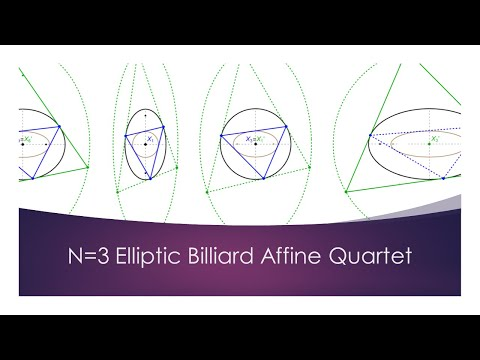
\includegraphics[width=.5\textwidth]{pics/EJzqsELkPN4.jpg}\end{center}
% From Left to Right:

First: A family of Poncelet 3-periodics (blue) in the elliptic billiard, i.e., interscribed in a pair of confocal ellipses (black and brown). Classical conservations include perimeter and Joachimsthal's constant [1].  This family also conserves the sum of internal angle cosines. Also shown are the excentral polygons (solid green); these conserve the product of internal angle cosines [2,3,4]. The ratio of areas of the excentral to that of 3-periodics is also conserved [5]. The locus of the excenters is an ellipse (dashed green). 

Second: the affine image of confocal family which sends the caustic to a circle. This family also conserves the sum of its cosines [3]. Surprisingly it is equal to that of its confocal pre-image (left). Notice the image of the original excentrals (green) does not conserve its product of cosines (grayed out). Note these are not the excentrals of the current family.

Third: the affine image of the confocal family which sends the outer ellipse to a circle (black). Like confocal excentrals, this also conserves the product of cosines [3]. Surprisingly it is equal to that of the excentrals. Also shown is the image of the confocal excentrals under the same affine transformation. This family has an incircle and like the previous one conserves its sum of cosines. Surprisingly, it is equal to the sum conserved by the original confocal family (first) and the one with incircle (second).

Fourth: the affine image of the confocal 3-periodics (first) which sends the locus of the excenters to a circle (dashed green). Like its confocal pre-image, this also conserves the product of its cosines [3]. Surprisingly it is equal to that of its confocal pre-image (first) and that of the family with incircle (third). These triangles are *not* the excentrals of the current family (blue) which do not conserve their sum of cosines (grayed out).

Experimentally, we have also noticed that the confocal+incircle families sweep the same curve in 3-dimensional "cosine space", as do the outer+circumcircle families, see [8].

[1] S. Tabachnikov, "Geometry and Billiards", Student Mathematical Library, vol 30, American Mathematical Society, 2005. http://www.personal.psu.edu/sot2/book...​
[2] D. Reznik, R. Garcia, and J. Koiller, "Can the Elliptic Billiard still surprise us?", Math Intelligencer, 42, 2020. http://rdcu.be/b2cg1​
[3] A. Akopyan, R. Schwartz, and S., "Billiards in Ellipses Revisited", Eur. J. Math, 2020. 
[4] M. Bialy and S. Tabachnikov, "Dan Reznik's Identities and More",
Eur. J. Math., 2020.
[5] A.C. Chavez-Caliz, "More About Areas and Centers of Poncelet Polygons" , Arnold Math J., 2020.
[6] R. Schwartz,  "The Poncelet grid", Advances in Geometry, 7:2, 2007.
[7] M. Levi and  S. Tabachnikov, "The Poncelet Grid and Billiards in Ellipses",Am. Math. Monthly,  114:10, 2007.
[8] D. Jaud, D. Reznik, and R. Garcia, "Poncelet Plectra: Harmonious Properties of Cosine Space", arXiv:2104.13174 , 2020.
\item \textbf{Affine images of billiard N-periodics IIa: N=5 quartet \& trio} (2m25s), 4/2021. \href{https://youtu.be/VQ4fB_s33HE}{\url{youtu.be/VQ4fB\_s33HE}}
\begin{center}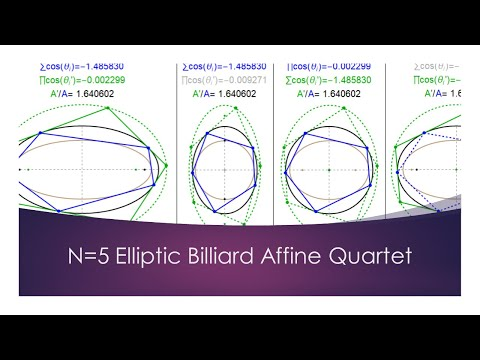
\includegraphics[width=.5\textwidth]{pics/VQ4fB_s33HE.jpg}\end{center}
% From Left to Right we see four animations (a Poncelet Quartet):

First: A family of Poncelet N-periodics (blue) in the elliptic billiard, i.e., interscribed in a pair of confocal ellipses (black and brown). We chose N=5 without loss of generality. Classical conservations include perimeter and Joachimsthal's constant [1]. This family also conserves the sum of internal angle cosines. Also shown are its ``outer´´ polygons (solid green) whose sides are tangent to the billiard at the N-periodic vertices; i.e., they run along each vertex's external bisector. The outer family conserves the product of internal angle cosines [2,3,4]. The ratio of areas of the outer polygon to that of 3-periodics is also conserved [5]. The locus of their vertices is an ellipse (dashed green), thanks to the Poncelet grid [6,7]. 

Second: the affine image of the billiard family which sends the caustic to a circle. This family also conserves the sum of its cosines [3], and it is equal to that of its confocal pre-image (left). Notice the image of the original outer polygons (dashed green) does not conserve its product of cosines (grayed out). Unlike the original outers, these do not have sides parallel to the external bisectors of corresponding N-periodic vertices. In N=3 parlance this would akin to saying "they are not excentral triangles".

Third: the affine image of the confocal family which sends the outer ellipse to a circle (black). Like confocal excentrals, this new family also conserves the product of cosines [3], and its value is equal to that of the confocal outer family. Also shown is the image of the confocal excentrals under the same affine transformation. This family circumscribes what is now a circle, i.e., it has a fixed incircle; like the previous one it conserves the sum of cosines, and surprisingly, it is equal to the sum conserved by the original confocal family (first) and the one with incircle (second), though none of these polygons is homothetic to one another nor do they have equal angle vectors (though we believe each sweeps the same curve in 5d angle or cosine space, see [8]).

Fourth: the affine image of billiard N-periodics (first) which sends the locus of outer vertices to a circle (dashed green). Like its confocal pre-image, this also conserves the product of its cosines [3], and it is equal to that of its confocal pre-image (first) and that of the family with incircle (third). 

[1] S. Tabachnikov, "Geometry and Billiards", Student Mathematical Library, vol 30, American Mathematical Society, 2005. http://www.personal.psu.edu/sot2/book...​
[2] D. Reznik, R. Garcia, and J. Koiller, "Can the Elliptic Billiard still surprise us?", Math Intelligencer, 42, 2020. http://rdcu.be/b2cg1​
[3] A. Akopyan, R. Schwartz, and S., "Billiards in Ellipses Revisited", Eur. J. Math, 2020. 
[4] M. Bialy and S. Tabachnikov, "Dan Reznik's Identities and More",
Eur. J. Math., 2020.
[5] A.C. Chavez-Caliz, "More About Areas and Centers of Poncelet Polygons" , Arnold Math J., 2020.
[6] R. Schwartz,  "The Poncelet grid", Advances in Geometry, 7:2, 2007.
[7] M. Levi and  S. Tabachnikov, "The Poncelet Grid and Billiards in Ellipses",Am. Math. Monthly,  114:10, 2007.
[8] D. Jaud, D. Reznik, and R. Garcia, "Poncelet Plectra: Harmonious Properties of Cosine Space", arXiv:2104.13174 , 2020.
\item \textbf{Affine images of billiard N-periodics Ib: N=3 trio} (2m25s), 4/2021. \href{https://youtu.be/HjBZdrR3Azs}{\url{youtu.be/HjBZdrR3Azs}}
\begin{center}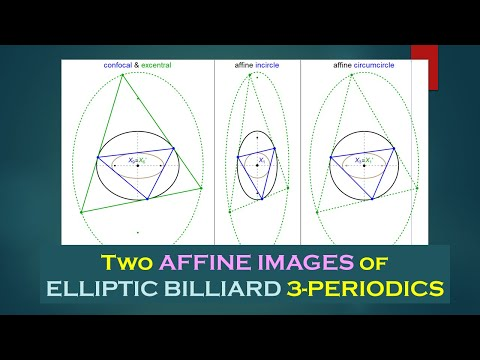
\includegraphics[width=.5\textwidth]{pics/HjBZdrR3Azs.jpg}\end{center}
% Left: A family of elliptic billiard 3-periodics (blue), i.e., , interscribed in a confocal pair of  ellipses (black and brown). This classically conserves perimeter and Joachimsthal's constant [1].  It turns out it also conserves the sum of internal angle cosines; furthermore, the Ponceletian family of its excentral polygons (green, inscribed in the dashed-green ellipse) conserves the product of its internal angle cosines [2,3,4]. The ratio of areas of the outer polygon to that of 3-periodics is also conserved [5]. Curiously, the excentrals also conserve the ratio of squared sidelengths by the product of sidelengths.

Middle: the affine image of billiard 3-periodics which sends the confocal caustic to a circle. This family also conserves the circumradius (not shown) and therefore the sum of its cosines [3]. Surprisingly, the latter is equal to that of its confocal pre-image (left). No conservations are known for its outer polygon (dashed green). Note these are affine images of confocal  excentrals, but are *not* excentrals of the current family.

Right: affine image of the confocal 3-periodics which sends the elliptic billiard to a circle (black). This also conserves the product of its cosines [3]. Surprisingly it is equal to the value conserved by the confocal excentrals (solid green, left). The caustic to its outer family (solid green) is a cirlce, i.e., this conserves the sum of cosines. Surprisingly, it is the same quantity conserved by the original billiard family.

[1] S. Tabachnikov, "Geometry and Billiards", Student Mathematical Library, vol 30, American Mathematical Society, 2005. http://www.personal.psu.edu/sot2/book...​
[2] D. Reznik, R. Garcia, and J. Koiller, "Can the Elliptic Billiard still surprise us?", Math Intelligencer, 42, 2020. http://rdcu.be/b2cg1​​
[3] A. Akopyan, R. Schwartz, and S., "Billiards in Ellipses Revisited", Eur. J. Math, 2020. 
[4] M. Bialy and S. Tabachnikov, "Dan Reznik's Identities and More",
Eur. J. Math., 2020.
[5] A.C. Chavez-Caliz, "More About Areas and Centers of Poncelet Polygons" , Arnold Math J., 2020.
[6] R. Schwartz,  "The Poncelet grid", Advances in Geometry, 7:2, 2007.
[7] M. Levi and  S. Tabachnikov, "The Poncelet Grid and Billiards in Ellipses",Am. Math. Monthly,  114:10, 2007.
\item \textbf{Affine images of billiard N-periodics IIb: N=5 role reversal} (2m25s), 4/2021. \href{https://youtu.be/7KtTtXXJlEI}{\url{youtu.be/7KtTtXXJlEI}}
\begin{center}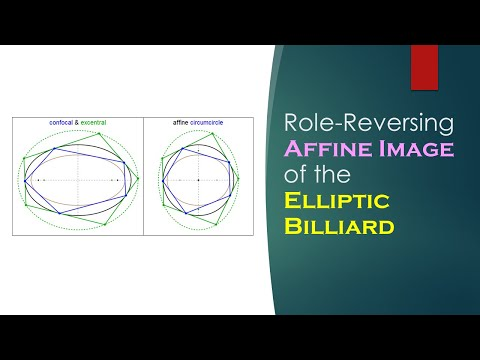
\includegraphics[width=.5\textwidth]{pics/7KtTtXXJlEI.jpg}\end{center}
% Left: family of Poncelet N-periodics (blue) in the elliptic billiard (black). N=5 case shown without loss of generality. Also shown is the outer polygon (solid green) whose sides are tangent to the billiard at the N-periodic vertices. The Poncelet grid implies this family will be inscribed in an ellipse (dashed green), i.e., the outer polygons are also a Poncelet family. While N-periodics conserve the sum of cosines, the outer family conserves the product of its cosines.

Right: the affine image of the confocal family which sends the billiard ellipse to a circle. A curious "role reversal" takes place here: (i) the circle-inscribed affine image of billiard N-periodics (blue) now conserves the product of cosines, and its value is equal to that conserved by the outer polygons in the pre-image. (ii) The affine image of the outer family (solid green) contains a fixed incircle. It too conserves the sum of its cosines, and its value is the same as the sum of cosines conserved by the original affine image.

Note that due to the affine transform there are no homothetic polygons.

Experiments also show that the (confocal, affine outer) pair not only conserves the same sum of cosines, but sweep the same curve in 5-dimensional cosine space. Likewise for the (confocal outer, confocal affine) -- not only these conserve the same product of cosines but sweep the same curve in 5-dim cosine space.
\end{enumerate}

\section{Anticevian (2)}

\begin{enumerate}[resume]
\item \textbf{The Anticevian Polygon I: Basic Phenomena} (13m18s), 1/2021. \href{https://youtu.be/FKvDfamTy-Y}{\url{youtu.be/FKvDfamTy-Y}}
\begin{center}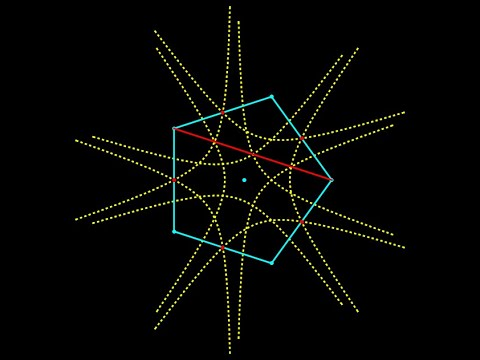
\includegraphics[width=.5\textwidth]{pics/FKvDfamTy-Y.jpg}\end{center}
% Recall the anticevian triangle T' of a reference triangle T wrt point X is such that T is the cevian of T' wrt X [1]. 

Here we extend this notion to N-gons, where N is odd.

First define the X-cevian polygon of an N-gon P as having vertices at the intersections of lines Pi X with sides of P opposite to Pi. For example, P3P4 is opposite to P1, P4P5 to P2, etc.

Now define P', the X-anticevian of P: it is such such that P is the X-cevian of P'. 

Unlike the cevian calculation, which is direct and local (it only requires a vertex and the opposing side), obtaining the vertices of the anticevian requires global information. A. Akopyan has suggested a very clever algorithm based on the composition of projectivities we shall explain elsewhere.

The video shows  the dynamic geometry of both the cevian and anticevian as a point X is dragged around in the plane of a regular pentagon.

When bounded (see below), the anticevian can be convex, concave, self-intersection.

The video also shows that if X is on a certain web of hyperbola-like curves (10 branches total), one or more vertices of the anticevian go to infinity. This web divides the plane into "cells". If X remains within one such cell, the vertices of the anticevian remain bounded, and its area function is continuous.

Note: in the video I say every such branch goes thru a side midpoint, of course this is wrong. In fact, every *pair* of branches has one branch which goes thru sides' midpoint.

The viewer is also invited to interact with a (slow) wolfram app we published on the web [2].

[1] E. Weisstein, Anticevian Triangle, Mathworld, 2021. https://mathworld.wolfram.com/AnticevianTriangle.html
[2] D. Reznik, Anticevian App, Wolfram Cloud, 2021. http://bit.ly/3oKUVf5
\item \textbf{The Anticevian Polygon II: Cyclical Projectivities} (9m18s), 1/2021. \href{https://youtu.be/BLHBlOWrtjs}{\url{youtu.be/BLHBlOWrtjs}}
\begin{center}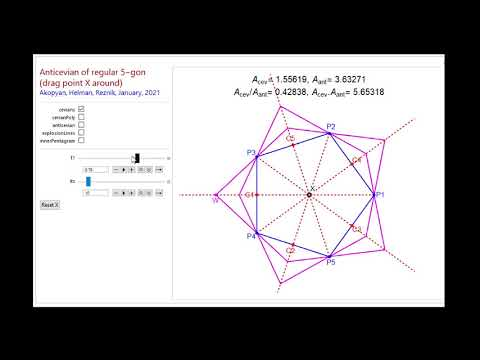
\includegraphics[width=.5\textwidth]{pics/BLHBlOWrtjs.jpg}\end{center}
% This is a continuation of our previous video on the anticevian polygon. We demonstrate that the anticevian is obtained as the composition of projectivities. We also demonstrate what happens to this iteration when the starting point W is not chosen at the correct location of a first vertex Q1 of the anticevian. After N iterations, we get a non-closing path. However, if N additional iterations are executed, we are taken back to W. We show the correct anticevian is a degenerate case where the two wraparound paths are identical.

The viewer is encouraged to interact with this experiment by going to [2].

[1] D. Reznik, "The Anticevian Polygon I: Basic Phenomena", YouTube, 2021. https://youtu.be/FKvDfamTy-Y
[2] D. Reznik, Anticevian App, Wolfram Cloud, 2021. http://bit.ly/3oKUVf5
\end{enumerate}

\section{Area Invariants (3)}

\begin{enumerate}[resume]
\item \textbf{Amazing Ellipse Pedal and Contrapedal Curves: area invariance for all pedal points on a circle!} (7m20s), 6/2020. \href{https://youtu.be/UUnvj7VIYso}{\url{youtu.be/UUnvj7VIYso}}
\begin{center}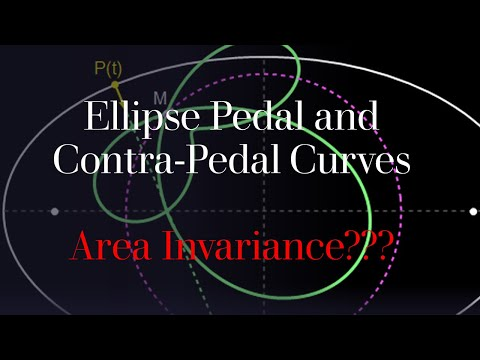
\includegraphics[width=.5\textwidth]{pics/UUnvj7VIYso.jpg}\end{center}
% Let C be a curve (in our case an ellipse, but it can be anything) and M a point in the plane. The pedal (resp. contrapedal) of C with respect to M is the locus of the foot of perpendiculars dropped from M onto tangents (resp. normals) to C passing through P on C, for all P on C [1,2].

The video makes an observation that may or may not be known:

Both the pedal and contrapedal curves of an ellipse E have *invariant* signed areas, so long as M rides on a circle concentric with E. It made me jump off my chair! The signed area counts self-intersecting loops of the curve as negative [3]. 

This is probably a known identity: let A, A_p, and A_c denote the area of the ellipse, the pedal curve, and the contra-pedal, the latter two with respect to the same point M. 

A_p = A + A_c

I.e., if the phenomenon of invariance with respect to all M on a concentric circle holds for the pedal its hould also hold for the contra-pedal.

P.S. - during the part I cover the "pedal"  I keep incorrectly calling it an "evolute". The ellipse evolute is a different beast [4], though the contra-pedal curve can also be computed as the pedal to the evolute. Sorry about the confusion.

[1] Mathworld, "Pedal Curve", https://mathworld.wolfram.com/PedalCurve.html
[2] Mathworld, "Antipedal Curve", https://mathworld.wolfram.com/ContrapedalCurve.html
[3] Mathworld, "Polygon Area", https://mathworld.wolfram.com/PolygonArea.html
[4] Mathworld, "Ellipse evolute", https://mathworld.wolfram.com/EllipseEvolute.html
\item \textbf{Regular Polygons: the Signed Area of the Antipedal Polygon Vanishes along a Circle?} (18m4s), 6/2020. \href{https://youtu.be/9PZ6_bHz2UE}{\url{youtu.be/9PZ6\_bHz2UE}}
\begin{center}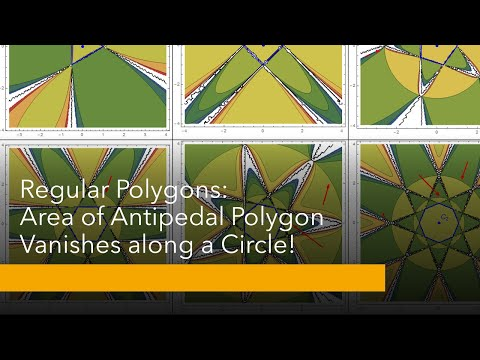
\includegraphics[width=.5\textwidth]{pics/9PZ6_bHz2UE.jpg}\end{center}
% Are there any new observations possible in the world of regular polygons?

Take a regular N-gon w center at O, N greater than 3. Consider a circle C1 centered on O with radius R1 = |Q-O|, where Q is the intersection of side i with side i+2 of the N-gon.

1) For P on any circle centered on O, the pedal polygon [3,*] of the N-gon wrt to P has constant area. This result was proven by J. Steiner in 1825 [1]. This builds on an 1823 proof by Sturm applied to triangles [2].

2) New observation: the signed area of the antipedal polygon [4,**] of the N-gon with respect to P is constant and equal to ZERO, for all P on C1.

2.1) For N=7 (and 8) you can find a 2nd circle C2 centered on O and with radius R2=|Q'-O|, where Q' is the intersection of side i with side i+3. Observation (2) also holds for P on C2.

2.2) For higher N there are more such circles.

Notes:

(*) The pedal polygon are the feet of perpendiculars dropped from P onto the sides.
(**) The antipedal polygon has sides through the vertices of the N-gon and perpendicular to lines drawn from P onto the vertices of the N-gon
References: 

[1] Steiner's Theorem (1825) for constant area pedal polygons -- http://users.math.uoc.gr/~pamfilos/eGallery/problems/PedalPolygons.html
[2] Ostermann et al, "Geometry and Its History", Sturm's Theorem, https://books.google.com.br/books?id=eOSqPHwWJX8C&pg=PA221&lpg=PA221&dq=sturm%27s+theorem+area+pedal&source=bl&ots=nj4PosDX0w&sig=ACfU3U0iSH7An02LbgdCdYMwkPN290P0rQ&hl=en&sa=X&ved=2ahUKEwit-9bVnajqAhUFIrkGHTZFAnwQ6AEwCHoECAoQAQ#v=onepage&q=sturm's%20theorem%20area%20pedal&f=false

[3] Pedal Triangle, https://mathworld.wolfram.com/PedalTriangle.html 
[4] Antipedal Triangle, https://mathworld.wolfram.com/AntipedalTriangle.html
\item \textbf{Steiner's Krümmungs-Schwerpunkt implies Area-Invariant Interpolated Pedal Curve over Circles} (1m6s), 9/2020. \href{https://youtu.be/gR8Axe823_M}{\url{youtu.be/gR8Axe823\_M}}
\begin{center}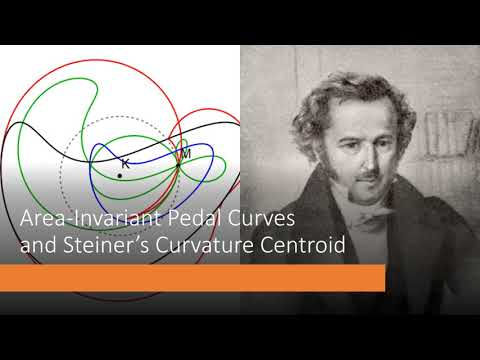
\includegraphics[width=.5\textwidth]{pics/gR8Axe823_M.jpg}\end{center}
% Top left: a generic concave curve C (black) is shown as well as its curvature centroid K. A point M is shown lying on a circle (dashed black) centered on K. Also shown are the pedal Cc (red) and contrapedal Cp (green) curves of C with respect to M. These are animated for varying positions of M on the circle centered on K. Notice their areas Ap and Ac are invariant.

Top right: the interpolated pedal curve Cμ (blue) for μ=1/4 . Cμ = (1-μ)Cp + μ Cc. Surprisingly, its area Aμ is also invariant for M on a circle centered on K.

Bottom left: μ=1/2. Here Cμ will be homothetic to C (at a scale of 1/2) and its area is independent of the location of M.

Bottom right: Cμ is shown for μ=3/4, isocurves of invariant Aμ are as before, circles centered on K.

These facts are proven in [1].

References.

[1] D. Reznik, R. Garcia, Hellmuth Stachel, "New Area-Invariant Pedal-Like Curves Associated with the Ellipse", arXiv
\end{enumerate}

\section{Bicentric Family (10)}

\begin{enumerate}[resume]
\item \textbf{Non-Concentric Circular Poncelet Pair: Invariant Sum of Japanese Theorem Inradii (A. Akopyan)} (1m47s), 10/2020. \href{https://youtu.be/BEvdUUolUXI}{\url{youtu.be/BEvdUUolUXI}}
\begin{center}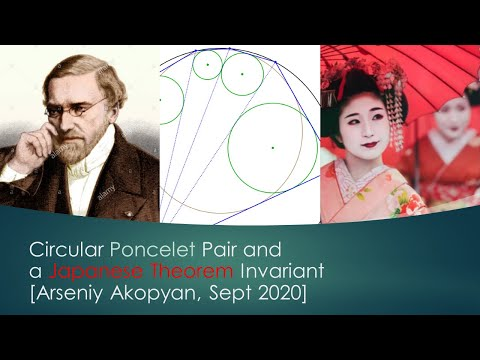
\includegraphics[width=.5\textwidth]{pics/BEvdUUolUXI.jpg}\end{center}
% The video shows (for N=5,6) a conjecture by A. Akopyan [2]. Over the Bicentric family, i.e., Poncelet N-gons interscribed between two non-concentric circles, the sum of the inradii of the triangles in a tesselation of said N-gons is invariant.  

Recall the so-called "Japanese Theorem" [1] to which this is related: given a convex, circle-inscribed polygon P with N vertices, subdivide it in subtriangles. The Japanese Theorem states the sum of the inradii of said subtriangles is invariant over the particular subdivision picked.

[1] E. Weisstein, "Japanese Theorem", Mathworld. https://mathworld.wolfram.com/JapaneseTheorem.html
[2] A. Akopyan, "Japanese Thm Invariant Inradius Sum for Non-Concentric Circular Poncelet", Private Comm., Oct 11, 2020.
\item \textbf{Bicentric Family I: Properties of Pedals, Polars, \& Inversions of N-Periodics in Elliptic Billiard} (PT19M), 2/2021. \href{https://youtu.be/jhXDKRFLpVk}{\url{youtu.be/jhXDKRFLpVk}}
\begin{center}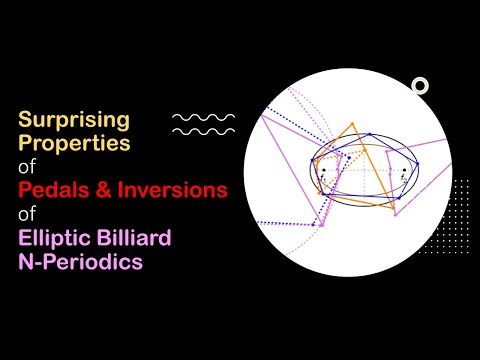
\includegraphics[width=.5\textwidth]{pics/jhXDKRFLpVk.jpg}\end{center}
% Video shows a number of phenomena related to pedals, and inversions of N-periodics in the elliptic billiard. The main result is that there are two sequences of 3 operations which take the original N-periodic to a translated copy of itself. Theses are:

Path 1. pedal+pedal+inversion

1.1) the f1-pedal to N-periodics is a bicentric family inscribed in a circle whose radius is equal to the major axis of the caustic. To be proved: bicentric families conserve the sum of cosines.
1.2) the f1-pedal to (1.1), i.e., the "squared" f1-pedal, is equiperimeter and homothetic to the f2-inversive family. these families are inscribed in Pascal's Limaçon (not shown), and both have identical invariant sum of cosines.
1.3) the f1-inversion of (1.2) produces a copy of N-periodics translated by (-2c,0), where c is the original focal distance sqrt(a^2-b^2).

Path 2. inversion+antipedal+antipedal

2.1) the f1-inversion of N-periodics produces an invariant perimeter family whose invariant sum of cosines is identical to (1.2).
2.2) the f1-antipedal of (2,1) produces a bicentric family which conserves the sum of cosines, identical to the sum of cosines of (1.1). Additionally, the product of its area with that of (1.1) is constant.
2.3) the f1-antipedal of (2.2), i.e., the "squared" f1-antipedal produces a family identical to (1.3).

Errata:

- at 5:15: "the two perimeters are identical": what's meant is that they are both *invariant*
- at 14:18: the numerics are correct in that it is the *product* of areas of the two bicentric families, (i) f1-pedal and (ii) polar which is conserved. notice these families are "out of phase, mirrored" coopies of each other and their sum of cosines is identical.
\item \textbf{Bicentric Family II: invariant perimeter limiting point pedals} (13m21s), 2/2021. \href{https://youtu.be/A7F3szW7rUE}{\url{youtu.be/A7F3szW7rUE}}
\begin{center}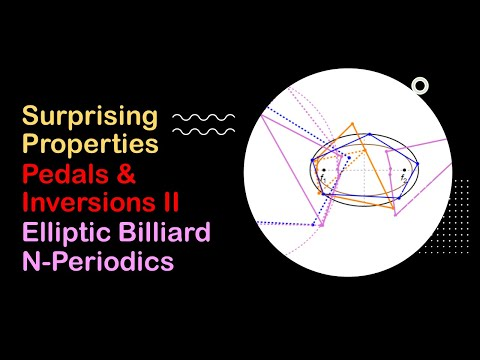
\includegraphics[width=.5\textwidth]{pics/A7F3szW7rUE.jpg}\end{center}
% Consider N-periodics in the elliptic billiard w/ foci at f1 and f2. A polar transformation wrt f1 sends the billiard family to a bicentric "polar" family where f1 is one of its limiting points [1]. Therefore, the invariant-perimeter f1-inversive polygon can be regarded as the pedal of the polar family wrt to f1. 

obs 1: the polar family  conserves the sum of cosines.
obs 2: the f1-inversives conserve perimeter. It also conserves sum of cosines (except when N=4).
obs 3: let l2 denote the 2nd limiting point of the bicentric pair. the pedal of the bicentrics wrt to l2 also conserves perimeter and sum of cosines (no exceptions).

Each of the two bicentric pedal families (wrt f1 or l2) rides on a separate limaçon of Pascal. The f1 one is loopless, whereas the second limaçon has a loop which goes thru l2.

obs 4: For N=4 the l2-bicentric-pedal degenerates to a segment
obs 5: for N=3, the f1- and l2-pedals are similar triangles (modulo reflection), and all their sum of cosines is equal to that of the bicentric (poristic) family. This implies all 3 families have identical and invariant r/R. Note that the  r/R of billiard 3-periodics is also invariant but different from the trio's.

[1] E. Weisstein, "Limiting Point", MathWorld, 2021. https://mathworld.wolfram.com/LimitingPoint.html
\item \textbf{Bicentric Family III: Equiperimeter ``Limiting'' Pedal Polygons to the Bicentric Family} (25m53s), 2/2021. \href{https://youtu.be/6TmaezNFrOs}{\url{youtu.be/6TmaezNFrOs}}
\begin{center}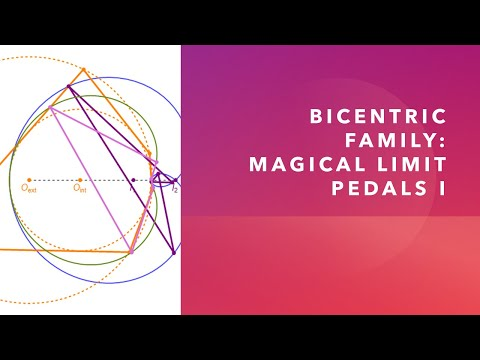
\includegraphics[width=.5\textwidth]{pics/6TmaezNFrOs.jpg}\end{center}
% The video narrates several curious properties of the bicentric family [1] and its pedal polygons wrt to its limiting points l1 and l2 [2] i.e., the two points wrt which the inversion of the bicentric circle pair yields a concentric pair (I messed up in the video, sorry). The video shows that

a) the sum of cosines of bicentrics is conserved.
b) limiting pedals are inscribed in separate, touching Pascal Limaçons, one loopless and the other with a loop through l2.
c) the perimeter of both limiting pedals is invariant.
d) the sum of cosines of both limiting pedals is invariant (except for when N=4, where the l1-pedal has variable sum of cosines).
e) in the N=4 case,  the vertices of the l2-pedal are collinear.
f) in the N=3 case the bicentrics are the poristic family [3]. The sum of cosines of bicentrics, l1- and l2-pedals are the *same*. Their Gergonne point X7 is stationary.

For (f) we prepared a set of animations here: dan-reznik.github.io/ellipse-mounted-loci-p5js/?juke=6

Note: over the poristic family, the Gergonne point X7 moves along a circle [3].

[1] E. Weisstein, "Poncelet Porism", MathWorld, 2021. https://mathworld.wolfram.com/PonceletsPorism.html
[2] E. Weisstein, "Limiting Points", MathWorld, 2021. https://mathworld.wolfram.com/LimitingPoint.html
[3] B. Odehnal, "Poristic Loci of Triangle Centers, Journal for Geometry and Graphics 15(1) , 2010.
\item \textbf{Bicentric Family IV: Constant-Perimeter Limiting Point Pedals in the N=4 Case} (10m45s), 3/2021. \href{https://youtu.be/fZe6elRTfeA}{\url{youtu.be/fZe6elRTfeA}}
\begin{center}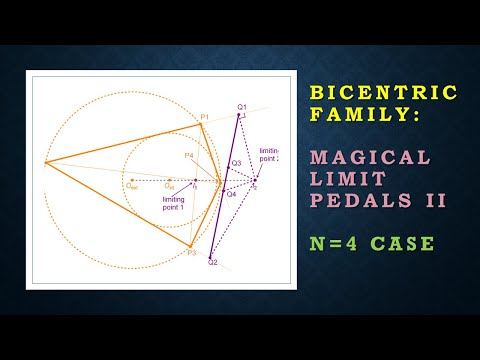
\includegraphics[width=.5\textwidth]{pics/fZe6elRTfeA.jpg}\end{center}
% The video describes properties of the Poncelet Bicentric family of quadrilaterals interscribed by two circles which can be calculated via Fuss's formula for N=4 [1, Eqn. (39)]. Let l1,l2 denote the two limiting points [2] of the circumcircle-incircle pair of the family. A well know result about bicentric polygons is that their diagonals meet at one of the limiting points.

The video showcases a few curious properties of the bicentrics' pedal polygons with respect to either l1 and l2, to be sure:

a) the l1-pedal has constant perimeter and its vertices sweep a loopless Pascal limaçon.
b) all 4 vertices of the l2-pedal are dynamically collinear (zero area) and sweep a Pascal limaçon whose loop has a node at l2. The perimeter of the l2-pedal is also constant and its sum of cosines is invariant and equal to 4.

[1] E. Weisstein, "Poncelet Porism", MathWorld, 2021. https://mathworld.wolfram.com/PonceletsPorism.html

[2] E. Weisstein, "Limiting Points, MathWorld, 2021. https://mathworld.wolfram.com/LimitingPoint.html
\item \textbf{Zero-Area N=4 Bicentric Pedals} (8m37s), 3/2021. \href{https://youtu.be/hwx1i-W6yLQ}{\url{youtu.be/hwx1i-W6yLQ}}
\begin{center}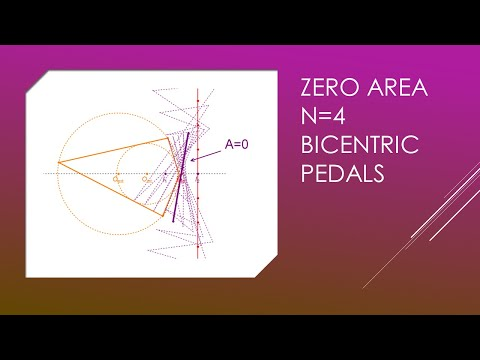
\includegraphics[width=.5\textwidth]{pics/hwx1i-W6yLQ.jpg}\end{center}
% Consider a N=4 Poncelet family of polygons (orange) interscribed between two nested circles, called here the N=4 bicentric family. We have shown recently this family conserves sum of cosines and the perimeter of pedal polygons wrt to either one of its limiting points [1].

Consider the family of pedal polygons of the bicentrics wrt to a generic point P0 in the plane. The video shows that if P0 lies on the line perpendicular to Oint and Oext and passing thru l2, the area of the bicentric pedal wrt to P0 is dynamically zero.

[1]  P. Roitman, R. Garcia, and D. Reznik, "New Invariants of Poncelet-Jacobi Bicentric Polygons", March 2021. https://bit.ly/2Qs3r6D
\item \textbf{The Jacobi-Poncelet Bicentric family: 3 derived constant perimeter families} (4m20s), 3/2021. \href{https://youtu.be/8m21fCz8eX4}{\url{youtu.be/8m21fCz8eX4}}
\begin{center}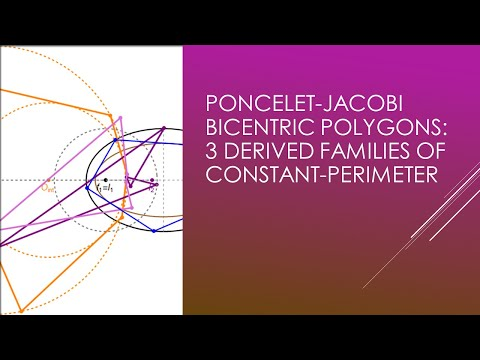
\includegraphics[width=.5\textwidth]{pics/8m21fCz8eX4.jpg}\end{center}
% This video supports our recent publication [1]. It shows the family of Poncelet-Jacobi bicentric polygons [2] and its two limiting points l1 and l2. It also shows the following three invariant perimeter families: 
a) the pedal polygon wrt l1, inscribed in a loopless Pascal Limaçon
b) the pedal polygon wrt l2, inscribed in a Pascal Limaçon which loops thru l2.
c) its polar image (N-periodics in the elliptic billiard with one focus on l1).

[1] P. Roitman, R. Garcia, and D. Reznik, "New Invariants of Poncelet-Jacobi Bicentric Polygons", 2021. https://arxiv.org/abs/2103.11260 
[2] E. Weisstein, "Poncelet Porism", MathWorld 2021. https://mathworld.wolfram.com/PonceletsPorism.html
\item \textbf{Peripheral triangles: circular locus of incenters and invariant sum of inradii} (2m26s), 7/2021. \href{https://youtu.be/HnqqaqDf2mo}{\url{youtu.be/HnqqaqDf2mo}}
\begin{center}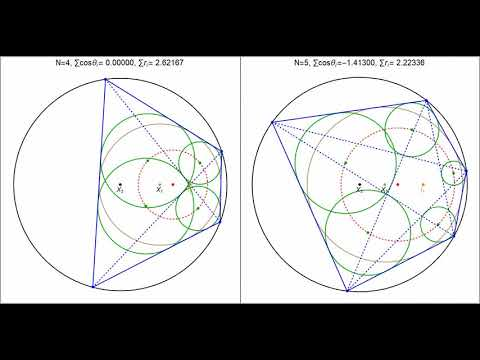
\includegraphics[width=.5\textwidth]{pics/HnqqaqDf2mo.jpg}\end{center}
% The video shows an N=4 (left) and N=5 (right) family of polygons (blue) interscribed between two circles C (black) and C' (brown), also known as bicentric polygons. Let Pi=1,...,N denote the vertices of each family. Let Ti = P(i)P(i+1)P(i+2) denote N "peripheral" subtriangles (dashed blue), where indices are computed (mod N). The video shows three properties:

a) the sum of internal angle cosines of a bicentric family is conserved (proved in [1]).
b) the sum of the inradii r(i) of the T(i) is conserved -- unproved for N greater than 4
c) the locus of the incenters of the T(i) is a circle (dashed red).
d) (Sept 1, 2021): the sum of 1/r(i) is also conserved!

[1] P. Roitman, R. Garcia, and D. Reznik, "New Invariants of Poncelet-Jacobi Bicentric Polygons",  Arnold Mathematical Journal, 2021 (to appear).
\item \textbf{Peripheral triangles: Constant Inradius Sum, Japanese-Style Triangles, Incenter Circular Loci} (2m26s), 7/2021. \href{https://youtu.be/TGwlfBUtKrs}{\url{youtu.be/TGwlfBUtKrs}}
\begin{center}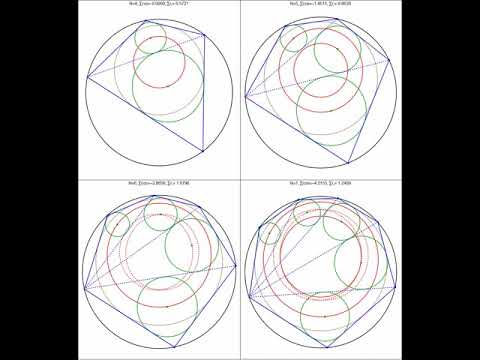
\includegraphics[width=.5\textwidth]{pics/TGwlfBUtKrs.jpg}\end{center}
% This is a result privately communicated to us by A. Akopyan, which we simulate here. A first video of this phemomenon appeared in [1].

The so-called "bicentric Poncelet" family is 1d family of polygons inscribed in an outer circle while simultaneously circumscribing a second inner circle. Recently we proved that  this family conserves the sum of its internal angle cosines [3].

Let the vertices of polygons in the family be labeled P1, P2, ..., PN. We call "japanese-style" triangulation (in reference to the much famed "japanese theorem" [2]) a subdivision in of an N-gon into N-2 triangles obtained as P(1)P(i)P(i+1), where i in [2,N-1] The original japanese theorem accepts any triangulation, but here we will stick to the just described "fan" style triangulation (all triangles share P1).

The video shows two phenomena. Over the bicentric family:

a) the sum of inradii is constant.
b) the locus of sum incenters (all in the N=4,5 cases, and some in the N=6,7 cases) are circles (solid reds). The remaining loci are non-conics (dashed red).

[1] https://youtu.be/BEvdUUolUXI
[2] https://mathworld.wolfram.com/JapaneseTheorem.html
[3] https://arxiv.org/abs/2103.11260 -- to appear, Arnold Math. J. 2021
\item \textbf{Circular locus of the covertices of an ellipse ``mounted'' to bicentric triangles} (3m55s), 12/2021. \href{https://youtu.be/wvNUdJbyHZA}{\url{youtu.be/wvNUdJbyHZA}}
\begin{center}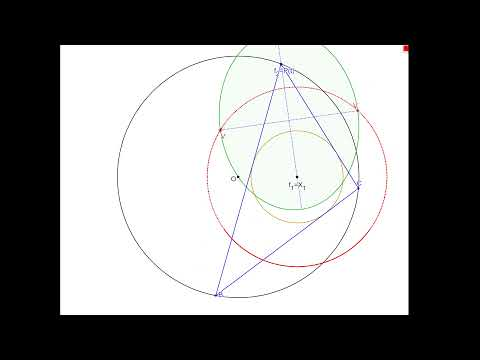
\includegraphics[width=.5\textwidth]{pics/wvNUdJbyHZA.jpg}\end{center}
% Consider the N=3 porism of "bicentric triangles", aka, Chapple's porism. These are triangles ABC inscribed in an outer circle C=(O,R) and circumscribing an inner circle C'=(I,r).

Now consider an ellipse E with foci on (I,A), constrained to pass thru O.

The video shows that over the porism, the locus of the two covertices of E is a marvellous circle.
\end{enumerate}

\section{Brocard (12)}

\begin{enumerate}[resume]
\item \textbf{Poncelet 3-Periodics of Homothetic Pair: Elliptic Loci of Brocard Pts + Vertices of 1st Brocard Tri} (1m37s), 9/2020. \href{https://youtu.be/13i3JGY-fK4}{\url{youtu.be/13i3JGY-fK4}}
\begin{center}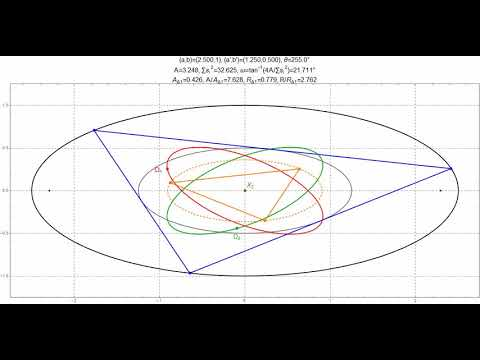
\includegraphics[width=.5\textwidth]{pics/13i3JGY-fK4.jpg}\end{center}
% Consider the family of Poncelet 3-periodics (blue) inscribed in an ellipse (a,b) and circumscribed about a concentric, axis-aligned caustic (a/2, b/2). This is known as the "homothetic pair". We have shown elsewhere [1] that this family conserves area, sum of squared sidelengths, and therefore Brocard angle.

The video shows the following additional properties:

a) the loci of the Brocard points Ω1 and Ω2 are two tilted, symmetric ellipses similar to the ones in the pair. These can be interior (a/b below 2.23...) or exterior to the caustic.
b) the locus of the vertices of the First Brocard Triangle (FBT) [2] is a horizontal ellipse, also similar to the ones in the pair. This is always interior to the caustic.
c) the area of the FBT is invariant
d) the ratio of 3-periodic circumradius to that of the FBT is invariant

[1] D. Reznik, "Poncelet 3-Periodics in the Homothetic Pair conserve Brocard angle", YouTube, 2020. https://youtu.be/2fvGd8wioZY
[2] E. Weisstein, "First Brocard Triangle", Mathworld 2020. https://mathworld.wolfram.com/FirstBrocardTriangle.html
\item \textbf{It takes 2 to tango: Brocard-Poncelet Porism, stationary Brocard Points and invariant Brocard Angle} (2m26s), 9/2020. \href{https://youtu.be/JANPPLET0so}{\url{youtu.be/JANPPLET0so}}
\begin{center}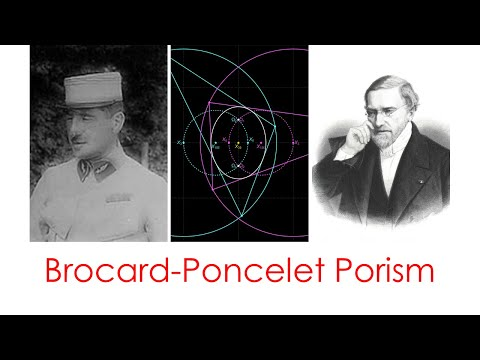
\includegraphics[width=.5\textwidth]{pics/JANPPLET0so.jpg}\end{center}
% Given an ellipse (a,b) (black) two Poncelet porisms can be set up for 2 families of 3-periodics (red and green triangles) of fixed circumcircle (and equal circumradius) such that E is their common caustic and their Brocard points (and their midpoint X39) are common and stationary. Also stationary for each family are X3, X6 and X182 (wrongly labeled X186 on video), the latter the center of the respective Brocard circles (shown dashed red and green).

It does take two to tango!

Acknowledgements: the vertices of isosceles configurations used to compute the porism were derived by Prof Ronaldo Garcia, on Sept 8, 2020.
\item \textbf{Joined at the hip: Brocard Porism, Steiner Ellipses, and the Homothetic Poncelet Pair} (4m1s), 9/2020. \href{https://youtu.be/h3GZz7pcJp0}{\url{youtu.be/h3GZz7pcJp0}}
\begin{center}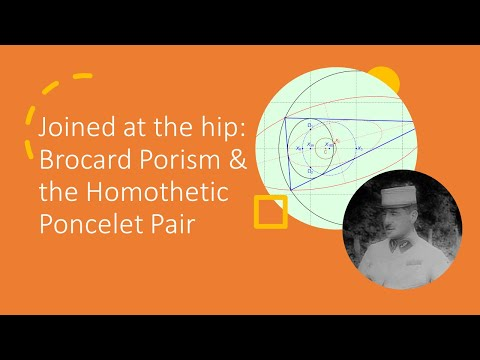
\includegraphics[width=.5\textwidth]{pics/h3GZz7pcJp0.jpg}\end{center}
% Consider Poncelet 3-periodics (blue) in the so-called Brocard Porism (external circumcircle and internal Brocard Inellipse -- the caustic). This remarkable triangle family has stationary Brocard points at the caustic foci, and is equibrocardal, i.e., it conserves Brocard angle ω. X3, X6, X39, X182, and several other triangle centers are also stationary (X15 and X16 to name a few).

Over the family, the animation shows:

a) the circular locus of the Barycenter X2 (brown), centered at "C" = X(11171) and of
radius = R*(2*Cos(2ω)-1)/3 (Peter Moses, 12-Sept-2020).
b) the Steiner ellipse (red) and inellipse (dashed red) to the 3-periodics. A key  property is that though its axes have variable length, their ratio is conserved. Notice its axes pass through the left and right extremes of the circle (a).

The corollary to (b) is that the Brocard porism can be regarded as an image of 3-periodics in the Homothetic Poncelet pair under a variable similarity transform (rigid translation and rotation + isotropic dilation), i.e., it is angle preserving. This is consistent with the fact that both systems conserve sum of cotangents.

Recall the homothetic pair actually conserves both L2 = sum of squared sidelenghts and area A, and therefore Brocard angle ω. The Brocard porism conserves the ratio of L2 and A, though neither is constant.
\item \textbf{The Poncelet Homothetic Pair contains an Aspect-Ratio Invariant Brocard Inellipse} (1m37s), 9/2020. \href{https://youtu.be/DIm2qTxGWXE}{\url{youtu.be/DIm2qTxGWXE}}
\begin{center}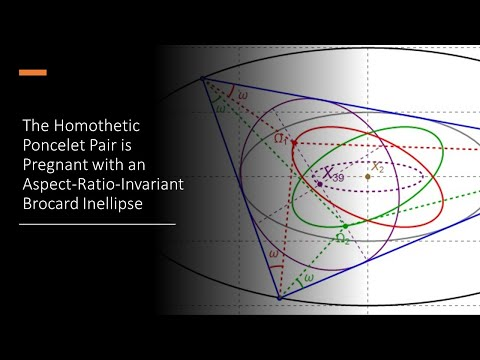
\includegraphics[width=.5\textwidth]{pics/DIm2qTxGWXE.jpg}\end{center}
% Shown are 3-periodics (blue triangles) interscribed in a homothetic poncelet pair: outer elipse (a,b), and inner one (a/2, b/2). The video shows a few phenomena.

1. Over the family, the sum of squared sidelenghts L2, area A and therefore Brocard angle ω = L2/(4A) are all invariant. The last property renders the family "equibrocardal".

2. The loci of the Brocard points Ω1,Ω2 are two marvellous titled ellipses (red, green), similar to the ones in the pair.

3. The family's Brocard inellipse (purple) [1] is centered on X39 and  Ω1,Ω2 lie on its foci. amazingly, its aspect ratio is invariant. What this implies is that there is a variable similarity transform between this family and the so-called Brocard porism, where 3-periodics are interscribed between a circle (their circumcirle) and the (stationary) Brocard inellipse. The converse image in the Brocard porism is that it conserves the aspec ratio of its Steiner Circumellipse, see [2].

4. The locus of X39 is an ellipse (dashed purple) whose axes (a39,b39) are (Ronaldo Garcia, Aug. 2020): a39 = (c2 a)/(2 (a^2 + 3 b^2)), b39 = (c2 b)/(2 (3 a^2 + b^2)), where c2=a^2-b^2.

[1] E. Weisstein, "Brocard Inellipse", MathWorld, 2020. https://mathworld.wolfram.com/BrocardInellipse.html 
[2] D. Reznik, "Brocard Porism", Youtube, 2020. https://youtu.be/h3GZz7pcJp0
\item \textbf{Brocard Porism: Locus of 1st, 2nd, 5th, and 7th Brocard Triangles' Vertices are Circles} (2m26s), 9/2020. \href{https://youtu.be/_bK-BCQv24A}{\url{youtu.be/\_bK-BCQv24A}}
\begin{center}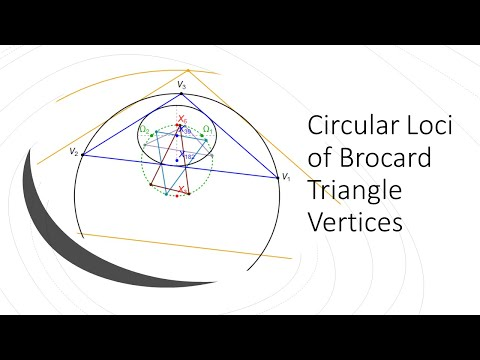
\includegraphics[width=.5\textwidth]{pics/_bK-BCQv24A.jpg}\end{center}
% The Brocard Porism [0] is a 1d family of Poncelet 3-periodics (blue) inscribed in a circle (black) and circumscribed about the Brocard inellipse (also black). Parametrics for their vertices were obtained from [1].

The 1st, 2nd, and 7th (*) Brocard Triangles [2] are know to be inscribed in the Brocard circle (green), and are concyclic with both Brocard points Ω1, Ω2, and X3, and X6. The 5th Brocard is homothetic to the reference, and its circumcenter is X9821 [3]. Therefore the locus of the vertices of the 1st, 2nd, and 7th are the Brocard circle itself, whereas that of the 5th is a circle centered on X9821. 

The loci of 3rd, 4th, and 6th triangles (not shown) are complicated curves.

You can also visualize these phenomena on our interactive app [4] here: https://bit.ly/32GFvQu

Note (*): The 7th Brocard Triangle was invented with Peter Moses in Sept. 2020.

References. 
[0] R. Johnson, "Advanced Euclidean Geometry" (Chapt XVII), Dover, 1960.
[1] R. Garcia, Vertices of Brocard-Poristic Triangles, Private Comm., Sept 2020.
[2] B. Gibert, CTC, https://bernard-gibert.pagesperso-orange.fr/gloss/brocardtriangles.html
[3] C. Kimberling, ETC (Part 5), 2020. https://faculty.evansville.edu/ck6/encyclopedia/ETCPart5.html
[4] I. Darlan and D. Reznik, Loci of Ellipse-Mounted Triangles, 2020, https://dan-reznik.github.io/ellipse-mounted-triangles/
\item \textbf{Rusian-doll nesting of Brocard porisms: concyclic sequence of Brocard points and the Beltrami points} (3m25s), 9/2020. \href{https://youtu.be/Z3YlEbCFbnA}{\url{youtu.be/Z3YlEbCFbnA}}
\begin{center}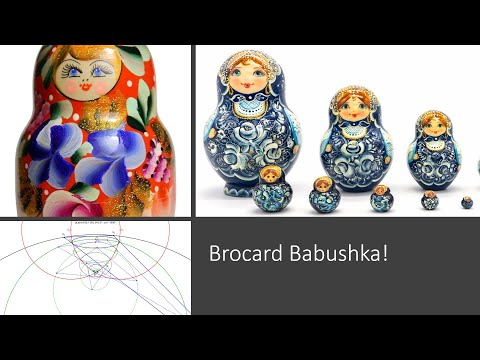
\includegraphics[width=.5\textwidth]{pics/Z3YlEbCFbnA.jpg}\end{center}
% The Brocard Porism [1] is a 1d Poncelet family of 3-periodics (triangles) inscribed in a circle and circumscribing their Brocard Inellipse [2]. Remarkably, the whole family has stationary brocard points Ω1 and Ω2 and fixed Brocard angle ω (Chapter XVII)[3].

The vertices of the Second Brocard Triangle T2 [4,5] are obtained by intersecting cevians through X6 with the Brocard circle, centered on X182 [6], i.e., T2 is inscribed in said circle.

It turns out that over the Brocard Porism, the Brocard points of T2 are also stationary [7]. Since they are inscribed in a circle, these define a "nested" Brocard porism.

The video shows such 4 iterations of such a nesting, whereby successive T2s are computed. Notice:

(1) successive Brocard inellipses tend to a shrinking circle
(2) successive T2's approach an ever shkring equilateral circumscribing
(3) the center of Brocard circles converges to a limit point. Could this be a triangle center?  
(4) the left (resp. right) sequence of Brocard points lies on a circle (shown red) centered on O2 (resp. O1), the first (resp. second) Beltrami point (circumcircle inverses of the Brocard points). The two circles have the same radius.

References:
 
[1] R. Bradley & G. Smith, "On a Construction of Hagge", Forum Geometricorum, vol 7, pp. 231-–247, 2007, url forumgeom.fau.edu/FG2007volume7/FG200730.pdf
[2] E. Weisstein, "Brocard Inellipse", Mathworld, 2020. https://mathworld.wolfram.com/BrocardInellipse.html
[3] R. Johnson, "Advanced Euclidean Geometry", Dover, New York, 1960. bit.ly/33cbrvd
[4] E. Weisstein, "Second Brocard Triangle", Mathworld, 2020. https://mathworld.wolfram.com/SecondBrocardTriangle.html
[5] B. Gibert, "Brocard Triangles", CTC, 2020. https://bernard-gibert.pagesperso-orange.fr/gloss/brocardtriangles.html
[6] C. Kimberling, "X(182)", ETC, 2020. https://faculty.evansville.edu/ck6/encyclopedia/ETC.html
[7] R. Garcia and D. Reznik, "Loci of the Brocard Points over Selected Triangle Families", arXiv, in preparation.
\item \textbf{Russian-Doll nesting of Brocard porisms courtesy of the second Brocard triangle} (3m13s), 9/2020. \href{https://youtu.be/T7c4CDHIk7s}{\url{youtu.be/T7c4CDHIk7s}}
\begin{center}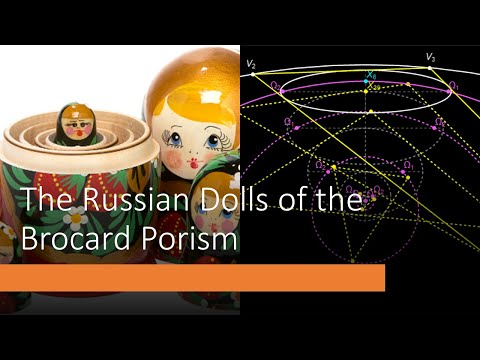
\includegraphics[width=.5\textwidth]{pics/T7c4CDHIk7s.jpg}\end{center}
% The Brocard Porism [1] is a 1d Poncelet family of 3-periodics (triangles) inscribed in a circle and circumscribing their Brocard Inellipse [2]. Remarkably, the whole family has stationary brocard points Ω1 and Ω2 and fixed Brocard angle ω (Chapter XVII)[3].

The vertices of the Second Brocard Triangle T2 [4,5] are obtained by intersecting cevians through X6 with the Brocard circle, centered on X182 [6], i.e., T2 is inscribed in said circle.

It turns out that over the Brocard Porism, the Brocard points of T2 are also stationary [7]. Since they are inscribed in a circle, these define a "nested" Brocard porism.

The video shows such 4 iterations of such a nesting, whereby successive T2s are computed. Notice:

(1) successive Brocard inellipses tend to a shrinking circle
(2) successive T2's approach an ever shkring equilateral circumscribing
(3) the center of Brocard circles converges to a limit point. Could this be a triangle center?  
(4) could all Brocard points lie on any interesting curve such as a parabola?

References:
 
[1] R. Bradley & G. Smith, "On a Construction of Hagge", Forum Geometricorum, vol 7, pp. 231-–247, 2007, url forumgeom.fau.edu/FG2007volume7/FG200730.pdf
[2] E. Weisstein, "Brocard Inellipse", Mathworld, 2020. https://mathworld.wolfram.com/BrocardInellipse.html
[3] R. Johnson, "Advanced Euclidean Geometry", Dover, New York, 1960. bit.ly/33cbrvd
[4] E. Weisstein, "Second Brocard Triangle", Mathworld, 2020. https://mathworld.wolfram.com/SecondBrocardTriangle.html
[5] B. Gibert, "Brocard Triangles", CTC, 2020. https://bernard-gibert.pagesperso-orange.fr/gloss/brocardtriangles.html
[6] C. Kimberling, "X(182)", ETC, 2020. https://faculty.evansville.edu/ck6/encyclopedia/ETC.html
[7] R. Garcia and D. Reznik, "Loci of the Brocard Points over Selected Triangle Families", arXiv, in preparation.
\item \textbf{Brocard Porism: equilateral Isodynamic Pedals have invariant area ratio + circular centroidal locus} (4m52s), 9/2020. \href{https://youtu.be/s4DF-iZZO8Y}{\url{youtu.be/s4DF-iZZO8Y}}
\begin{center}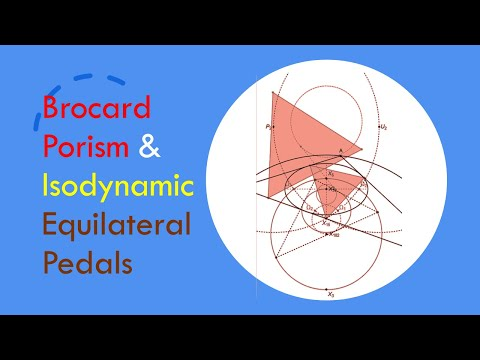
\includegraphics[width=.5\textwidth]{pics/s4DF-iZZO8Y.jpg}\end{center}
% A known property is that for any triangle, the pedal triangles of the isodynamic points X15, X16 is an equilateral. Here we study the dynamic geometry of said pedals over a special family of triangles known as the Brocard porism. The main takeaways are that, over said family, (1) the locus of the barycenters are two separate circles, and (2) the ratio of their areas is conserved. Also shown is a property likely true for any triangle: (3) the equilateral barycenters are collinear with the symmedian point X6.

The Brocard porism is a 1d Poncelet 3-periodic family (blue) inscribed in a circle (black) and circumscribed about an ellipse (black) known as the Brocard inellipse. Its two Brocard points Ω1,Ω2 are stationary on the latter's foci and the Brocard angle ω is conserved. The Brocard midpoint X39 is stationary. Also stationary are X3 (by definition) and X6, and the isodynamic points X15 and X16.

Containing Ω1,Ω2,X3,X6 is the (stationary) Brocard circle (green). It is centered on X182. Inscribed in it is the second Brocard Triangle (dashed blue) whose vertices are the intersections of cevians through X6 with the Brocard circle. Strikingly, second Brocards are a new Brocard porism, notice its stationary, smaller, less eccentric Brocard inellipse (gray). Its isodynamic points X15', X16' coincide with those of the original family. Furthermore, its first (resp. second) Brocard points Ω1',Ω2' is concyclic with Ω1, X15, X16 (resp. Ω2, X15, X16). These circles (dashed red) are centered on the Beltrami points P(2) and U(2), each of which is the circumcircle-intervers of Ω1,Ω2, respectively.
\item \textbf{Continuous Family of Brocard Porisms with Stationary Isodynamic Points $X_{15}$ and $X_{16}$} (1m20s), 9/2020. \href{https://youtu.be/jY_8zxBljuk}{\url{youtu.be/jY\_8zxBljuk}}
\begin{center}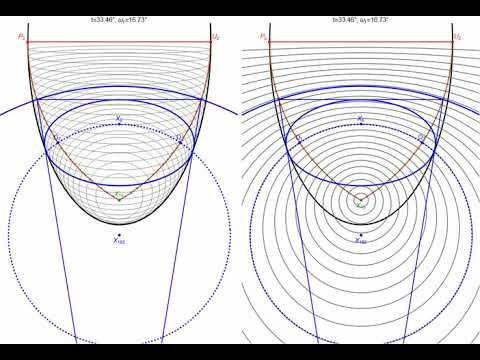
\includegraphics[width=.5\textwidth]{pics/jY_8zxBljuk.jpg}\end{center}
% A parameter t in 0 to pi/3 is used to parametrize a continous family of Brocard porisms, whereby the Brocard angles Ω1,Ω2 lie on two circular arcs (red) centered on the (fixed) Beltrami points P(2) and U(2).

Left: samples of the family of inellipses (gray) are shown having an elliptic envelope (thick black), with foci on the isodynamic points X15 (and X16, above the page, not shown). Picking a t amounts to selecting one inellipse and circumcircle (thick blue). The Brocard circle (dashed blue) is centered on X183, and contains both Brocard points Ω1,Ω2, X3 and X6. Both the latter and the circumcircle go start as an infinite circle (t=0), converging to X15 at t=pi/3. Notice the Brocard circle cuts the inellipse exactly where it touches the envelope. Notice the (fixed) Brocard angle ω of each porism is equal to t/2.

Right: inifnite nesting of the set of all circumcircles (gray) of the family. Notice these are perpendicular to the two Beltrami circles (red).
\item \textbf{The Family of Second Brocard Triangles in the Brocard Porism} (2m50s), 9/2020. \href{https://youtu.be/Wgwh4-neJp4}{\url{youtu.be/Wgwh4-neJp4}}
\begin{center}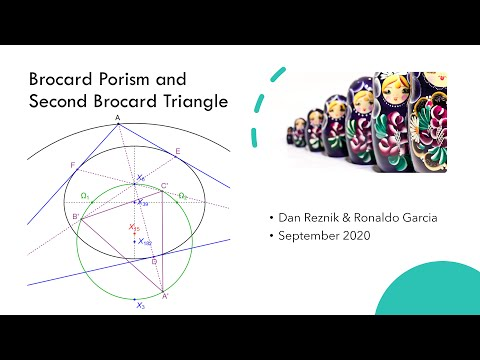
\includegraphics[width=.5\textwidth]{pics/Wgwh4-neJp4.jpg}\end{center}
% The Brocard porism is a 1d Poncelet family of triangles T=ABC (blue) inscribed in a circle Γ (black) and circumscribed about an inellipse E (black) known as the Brocard inellipse [1]. The Brocard points Ω1,Ω2 are stationary at the foci of E and the Brocard angle ω is invariant.

The Brocard circle K (green), which contains Ω1,Ω2,X3,X6 is stationary. The 2nd Brocard Triangle (purple) has vertices A'B'C' at the intersections of symmedians (cevians thru X6) with the Brocard circle [2]. It is therefore inscribed in K. Incredibly, the family of 2nd Brocard triangles is a new Brocard porism inscribed in K and circumscribed about a 2nd, smaller Brocard inellipse E' (not shown).

Also shown are the points of contact DEF of E to T: since X6 is the Brianchon point (perspector) of E [3], said points occur at the intersection of the symmedians with the sidelengths. Note also that the foci on an inellipse are isogonal conjugates, which is consistent with the fact that Ω1,Ω2 are such a pair. 

за здоро́вье!

[1] E. Weisstein, "Brocard Inellipse", Mathworld, 2020. https://mathworld.wolfram.com/BrocardInellipse.html
[2] E. Weisstein, "Second Brocard Triangle", Mathworld, 2020. https://mathworld.wolfram.com/SecondBrocardTriangle.html
[3] E. Weisstein, "Brianchon Point", Mathworld, 2020. https://mathworld.wolfram.com/BrianchonPoint.html
\item \textbf{Brocard Porism: Family of Second Brocard Triangles is a second Brocard Porism} (2m50s), 10/2020. \href{https://youtu.be/MprJtB4UW9s}{\url{youtu.be/MprJtB4UW9s}}
\begin{center}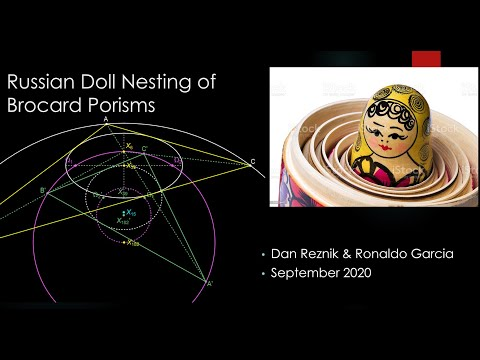
\includegraphics[width=.5\textwidth]{pics/MprJtB4UW9s.jpg}\end{center}
% The Brocard porism is a 1d Poncelet family of triangles T=ABC (blue) inscribed in a circle Γ (black) and circumscribed about an inellipse E (black) known as the Brocard inellipse [1]. The Brocard points Ω1,Ω2 are stationary at the foci of E and the Brocard angle ω is invariant. Also stationary are X15, and X16, the first and second Isodynamic points [4], though only the first one is shown. The Brocard circle K (green) contains Ω1,Ω2,X3,X6 and is stationary.

The 2nd Brocard Triangle T' (gold) has vertices A'B'C' at the intersections of symmedians (cevians thru X6) with the Brocard circle [2]. It is therefore inscribed in it.

One key observation borne out by the video is that the Brocard points  Ω1',Ω2' of T' are *also* stationary over the porism. Another known fact is that the isodynamic points of T' are congruent with those of T and are therefore also stationary.

But the main implication is that the family of 2nd Brocard triangles is a new Brocard porism inscribed in K and circumscribed about a 2nd, smaller Brocard inellipse E' (dashed black) of lower eccentricity than E. Interestingly, it can be shown the Brocard circle K' (dashed green) of this family is properly contained in K. 

If second Brocard triangles are computed recursively,  one obtains an infinite sequence of ever-smaller Brocard porisms which converge to the isodynamic point X15 common to all of them. Furthermore,  the sequence of Brocard circles K, K', K'', ..., form a Russian-doll (matryoshka) nesting which also shrinks to X15.

Note: also shown are the points of contact DEF of E to T: since X6 is the Brianchon point (perspector) of E [3], said points occur at the intersection of the symmedians with the sidelengths. Note also that the foci on an inellipse are isogonal conjugates, which is consistent with the fact that Ω1,Ω2 are such a pair. 

за здоро́вье!

[1] E. Weisstein, "Brocard Inellipse", Mathworld, 2020. 
[2] E. Weisstein, "Second Brocard Triangle", Mathworld, 2020. 
[3] E. Weisstein, "Brianchon Point", Mathworld, 2020. 
[4] E. Weisstein, "Isodynamic Points", Mathworld, 2020.
\item \textbf{Invariants of the Generalized Brocard Porism} (10m43s), 3/2021. \href{https://youtu.be/UYI_lBubKXA}{\url{youtu.be/UYI\_lBubKXA}}
\begin{center}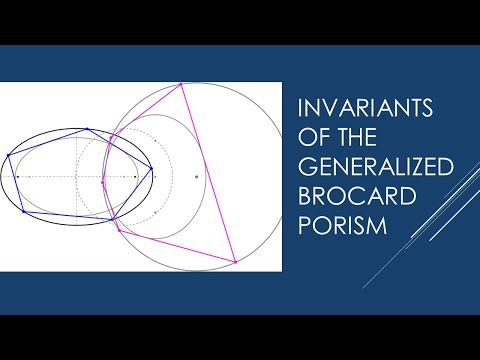
\includegraphics[width=.5\textwidth]{pics/UYI_lBubKXA.jpg}\end{center}
% This is joint work with Profs Ronaldo Garcia ad Pedro Roitman.

The "Brocard porism" is a family of triangles with fixed Brocard points and invariant Brocard angle [1]. The caustic is known as the "Brocard Inellipse", centered on X39. Its foci coincide with the stationary Brocard points of the family [4]. The symmedian point X6 of the family is also stationary [3] . We have studied the relationship between the Homothetic and Brocard family in [5]. 

The video shows that an N greater than 3 "generalized" Brocard porism (GBP) can be constructed as the polar image of the Poncelet homothetic family wrt to a circle C centered on one of the internal foci.

That the homothetic family conserves area is a trivial fact. Other conservations such as the sum of squared sidelengths, and sum of internal angle cotangents is proved in an upcoming paper [2].

The video shows that though the GBP does not conserve area, it conserves sum of inverse squared sidelengths AND sum of its angle cotangents (distinct from the former).

Erratum 1: in a parallelogram consecutive angles are supplementary (not opposing).

PS.1 -- the video does not mention a curious fact. For the N=3 case, the focus of the homothetic caustic where C is centered coincides with the (stationary) symmedian point X6 of the Brocard porism. You can also visualize the N=3 case live in your browser here: https://bit.ly/3tkDiEG

PS.2 -- the reason for null sum of cotangents in the N=4 generalized brocard porism (GBP) is because cyclic polygons have supplementary opposing angles.




References:

[1] C. Bradley, "The geometry of the Brocard axis and associated conics", CJB/2011/170, 2011, http://people.bath.ac.uk/masgcs/Article116.pdf
[2] S. Galkin, R. Garcia, and D. Reznik, "Invariants of Affine Images of Regular Polygons", to appear, 2021.
[3] D. Reznik and R. Garcia, "An Infinite, Converging, Sequence of Brocard Porisms", 2020. https://arxiv.org/abs/2010.01391
[4] E. Weisstein, "Brocard Inellipse", MathWorld, 2021. https://mathworld.wolfram.com/BrocardInellipse.html
[5] D. Reznik and R. Garcia, "Related By Similarity II: Poncelet 3-Periodics in the Homothetic Pair and the Brocard Porism", Intl. J. of Geom., 10(4), 2021, pp, 18--31.
\end{enumerate}

\section{Cayley-Poncelet (3)}

\begin{enumerate}[resume]
\item \textbf{Cayley-Poncelet Phenomena I: Finding an Ellipse Pair in General Position which admits 3-Periodics} (5m38s), 1/2021. \href{https://youtu.be/virCpDtEvJU}{\url{youtu.be/virCpDtEvJU}}
\begin{center}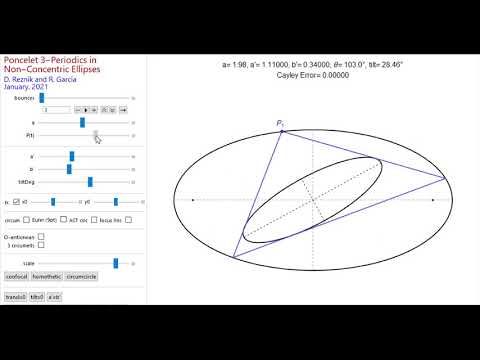
\includegraphics[width=.5\textwidth]{pics/virCpDtEvJU.jpg}\end{center}
% The video shows Poncelet 3-periodics in a pair of ellipses in "general position", namely,  the inner one need not be concentric nor axis-aligned with the outer one. Given the outer ellipse, we demonstrate how a numeric optimizer can be used to obtain the appropriate parameters for the inner ellipse such that the error associated with the Cayley condition vanishes.
\item \textbf{Cayley-Poncelet Phenomena II: Invariant Power of Center wrt Circumrcircle and Euler's Circle} (11m24s), 1/2021. \href{https://youtu.be/4xsm_hQU-dE}{\url{youtu.be/4xsm\_hQU-dE}}
\begin{center}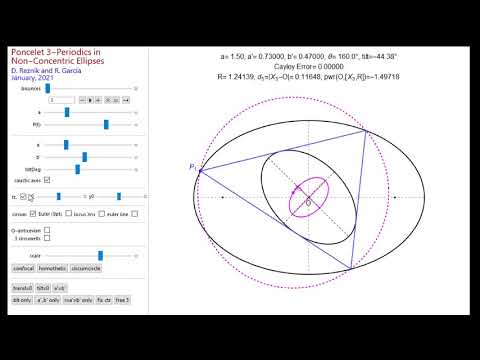
\includegraphics[width=.5\textwidth]{pics/4xsm_hQU-dE.jpg}\end{center}
% Take two concentric ellipses E and E' (axis-aligned or not) which admit a family of Poncelet 3-periodics (Cayley's condition is satisfied). Let the common center be O.

Let C3 (resp. C5) denote the circumcircle (resp. Euler's circle) of the family. These are centered on X3 and X5, respectively. Let their radii be R and R5. It is well-known R5=R/2.

The following observations are made. If E' and E are not axis-aligned:

a) the locus of X3 is an ellipse concentric and axis-aligned with E'.
b) the locus of X5 is an ellipse concentric but not axis-aligned with E'.
c) the power of O wrt C3 is invariant over the family.
d) the power of O wrt C5 is invariant over the family.

Note: in (a), and (b) the axes of the loci of X3 and X5 become axis aligned with the pair (E,E') is axis aligned itself.

If the pair is non-concentric, the locus of both X3 and X5 are still ellipses, though in general neither is axis-aligned with either E or E'. Also the power of O wrt to either C3 or C5 is no longer constant.
\item \textbf{Area Invariants of Poncelet N-Periodics and their Polar Polygons} (12m33s), 3/2021. \href{https://youtu.be/2TgmJ-YHydQ}{\url{youtu.be/2TgmJ-YHydQ}}
\begin{center}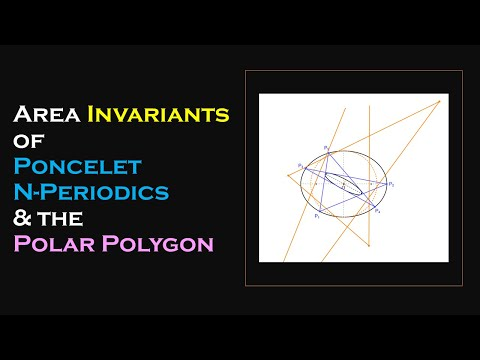
\includegraphics[width=.5\textwidth]{pics/2TgmJ-YHydQ.jpg}\end{center}
% Note: the invariants described in the video are a corollary of theorem 3 in [1] since the circle and polar polygon are invariant under the affine group.

The video shows several families of Poncelet N-periodics interscribed in concentric ellipse pairs which are not axis-aligned.

It also defines a "polar polygon" whose sides are bounded by the polars of the N-periodic vertices wrt to a fixed-radius circle concentric with the ellipses.

Let A  (resp. A') denote the area of the N-periodic (resp. polar polygon).

The main (experimental conjecture) is that over an N-periodic family, A/A' is invariant for all odd N, and A.A' is invariant for all N even.

[1] Arseniy Akopyan, Richard Schwartz & Serge Tabachnikov, "Billiards in Ellipses Revisited', European Journal of Mathematics, 2020. 

40 Accesses

0 Altmetric

Metrics

https://link.springer.com/article/10.1007/s40879-020-00426-9
\end{enumerate}

\section{Convex Combinations (3)}

\begin{enumerate}[resume]
\item \textbf{Barycenter with Median, and Incenter with Intouchpoint} (PT41S), 5/2019. \href{https://youtu.be/3Gr3Nh5-jHs}{\url{youtu.be/3Gr3Nh5-jHs}}
\begin{center}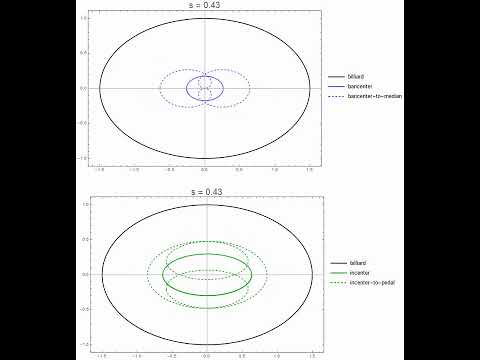
\includegraphics[width=.5\textwidth]{pics/3Gr3Nh5-jHs.jpg}\end{center}
% Elliptic loci of the barycenter (top) and incenter (bottom) for the family of 3-periodic orbits in an elliptic billiard is shown as solid curves. Dashed curves represent the convex combination of the former with a side's midpoint (respectively, an intouch/contact point). Notice how a perfectly elliptic locus deforms into one containing 3 windings, seemingly of 6th order.

For more information: https://dan-reznik.github.io/Elliptical-Billiards-Triangular-Orbits/
\item \textbf{Excenter and its corresponding Extouch point} (PT41S), 5/2019. \href{https://youtu.be/OD8Ah0hf8yQ}{\url{youtu.be/OD8Ah0hf8yQ}}
\begin{center}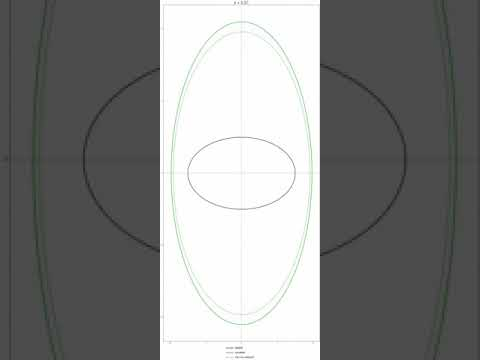
\includegraphics[width=.5\textwidth]{pics/OD8Ah0hf8yQ.jpg}\end{center}
% The three excenters of the family of 3-periodic orbits in elliptic billiards describe the same elliptic locus. Shown is the locus of the convex combination of one excenter with its corresponding extouch point (where the excircle touches a side), which happens to also be elliptic and congruent with the caustic.  Apparently, and unlike other convex combinations (barycenter and median, orthocenter and altitude foot, incenter and contact point), in this case all intermediate loci are elliptic.

For more information: https://dan-reznik.github.io/Elliptical-Billiards-Triangular-Orbits/
\item \textbf{Orthocenter with one altitude foot, and Circumcenter with median} (PT41S), 5/2019. \href{https://youtu.be/HZFjkWD_CnE}{\url{youtu.be/HZFjkWD\_CnE}}
\begin{center}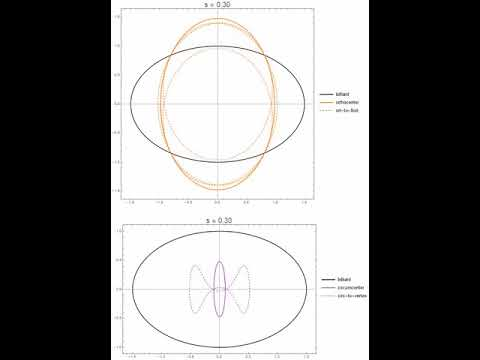
\includegraphics[width=.5\textwidth]{pics/HZFjkWD_CnE.jpg}\end{center}
% The orthocenter and/or circumcenter of the family of 3-periodic orbits in elliptic billiards are known to be ellipses. If we use a parameter "s" from 0 to 1 to dislocate either point toward one of its altitude feet (orbit vertex, respectively), their ellipses deform into higher order curves.

Elliptic loci of the orthocenter (top) and circumcenter (bottom) for the family of 3-periodic orbits in an elliptic billiard is shown as solid curves. Dashed curves represent the convex combination of the former with one altidude's foot (respectively, a vertex). Notice how a perfectly elliptic locus deforms into one containing 3 windings, seemingly of 6th order.

For more information: https://dan-reznik.github.io/Elliptical-Billiards-Triangular-Orbits/
\end{enumerate}

\section{Cross-Ratio Invariants (6)}

\begin{enumerate}[resume]
\item \textbf{Poncelet Cross-Ratio Invariants I: exploring N=5, 6, 7, 8} (37m29s), 2/2021. \href{https://youtu.be/vgHoLM5pg6o}{\url{youtu.be/vgHoLM5pg6o}}
\begin{center}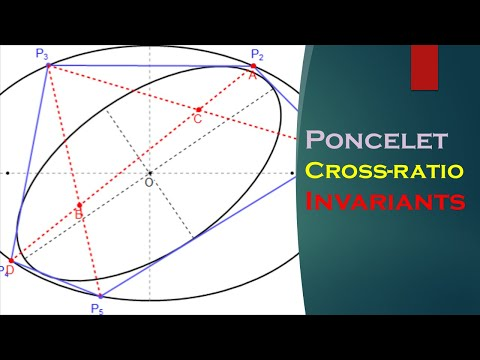
\includegraphics[width=.5\textwidth]{pics/vgHoLM5pg6o.jpg}\end{center}
% Recall the cross-ratio of 4 collinear points A,B,C,D  = (AC)(BD)/((BC)(AD)) [1]. There are 24 ways to order the four points, but only 6 groups of 4 combinations each yield distinct results, though all interrelated by simple expressions, see [1].

The video introduces several (possibly known) invariants in the sum (and/or product) of cross ratios defined over 3 "diagonals" in Poncelet N-Periodics. We cover N=5,6,7,8.

Comments appreciated!

[1] E. Weisstein, "Cross-Ratio", MathWorld, 2021. https://mathworld.wolfram.com/CrossRatio.html
\item \textbf{Poncelet Cross-Ratio Invariants II: 3 diagonals in the N=5 case} (7m42s), 2/2021. \href{https://youtu.be/XqpYVrXbK5s}{\url{youtu.be/XqpYVrXbK5s}}
\begin{center}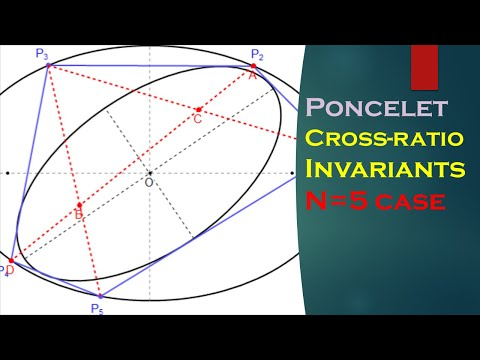
\includegraphics[width=.5\textwidth]{pics/XqpYVrXbK5s.jpg}\end{center}
% Consider the 1d family of Poncelet 5-periodics interscribed in a pair of non-concentric, non-aligned nested ellipses. Let Pi, i=1,...,5 be the vertices. Consider the following "diagonals" (i) P1P3, (ii) P1P4, and (iii) a "cross bar" diagonal P2 P5. Let four collinear points ABCD be defined as follows:

ABCD = P2, intersect(iii,i), intersect(iii,ii), P5.

The video explores the cross ratio of ABCD (or of 5 other orderings thereof).

Allow for ABCD to be defined as above, but with respect to any "starting" vertex Pi in the trajectory, i.e., some Pi takes the "role" of P1.

We show that under certain orderings, and over the 5-periodic family, the sum of cross ratios (wrt to each of the Pi), and/or the product of cross ratios, can be conserved
\item \textbf{Poncelet Cross-Ratio Invariants III: 3 diagonals in the N=5 self-intersected case} (8m58s), 2/2021. \href{https://youtu.be/4bd0YhQZMPM}{\url{youtu.be/4bd0YhQZMPM}}
\begin{center}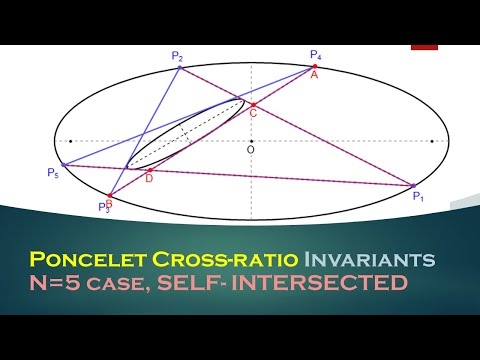
\includegraphics[width=.5\textwidth]{pics/4bd0YhQZMPM.jpg}\end{center}
% This is a follow-up on the previous video, where we are considering invariants resulting from sums and products of cross ratios defined by 3 diagonals in a Poncelet 5-periodic trajectory.

Here we consider the case of N=5 self-intersected and show its close relationship to the N=5 simple family.
\item \textbf{Poncelet Cross-Ratio Invariants IV: N=6 and N=8 and unit cross-ratio products} (13m20s), 2/2021. \href{https://youtu.be/i6krQu5Ls1E}{\url{youtu.be/i6krQu5Ls1E}}
\begin{center}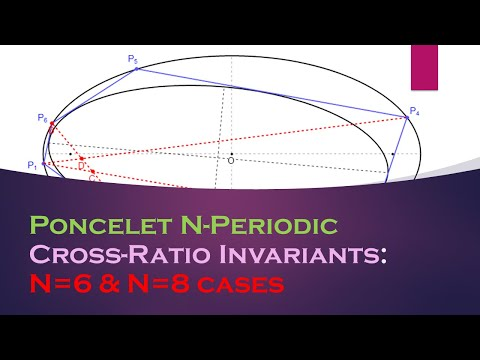
\includegraphics[width=.5\textwidth]{pics/i6krQu5Ls1E.jpg}\end{center}
% We demonstrate interesting invariants for products and sums of cross ratios in Poncelet 6- and 8-periodics.
\item \textbf{Poncelet Cross-Ratio Invariants V: Bicentric Pentagons, Pentagrams and their Projective Images} (23m55s), 2/2021. \href{https://youtu.be/b-WIfLej_yY}{\url{youtu.be/b-WIfLej\_yY}}
\begin{center}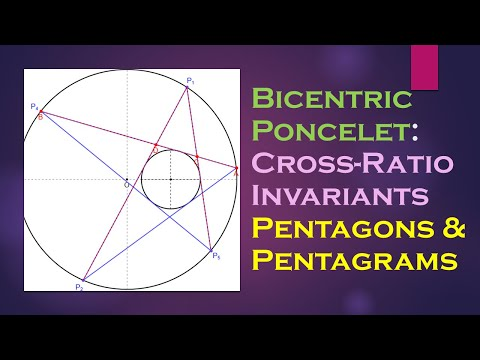
\includegraphics[width=.5\textwidth]{pics/b-WIfLej_yY.jpg}\end{center}
% This is not a Wicca video! We are actually describing interesting cross-ratio [1] related invariants manifested by over the Poncelet family of bicentric 5-gons (simple or self-intersected) [2]. Cross-ratios are measured on four collinear points obtained from certain diagonal (or chordal) arrangements between vertices in the trajectory. We show that the sum and product of cyclically-defined cross ratios are simultaneously invariant for 4 out 6 labeling of the collinear points.

Maybe this is a Wicca video after all...

[1] E. Weisstein, "Cross Ratio", MathWorld 2021.
[2] E. Weisstein, "Poncelet Porism", MathWorld 2021.
\item \textbf{Unit Product of Cross-Ratios in a Hexagon Independent of Vertices} (11m50s), 2/2021. \href{https://youtu.be/heiqfRTQ2Mc}{\url{youtu.be/heiqfRTQ2Mc}}
\begin{center}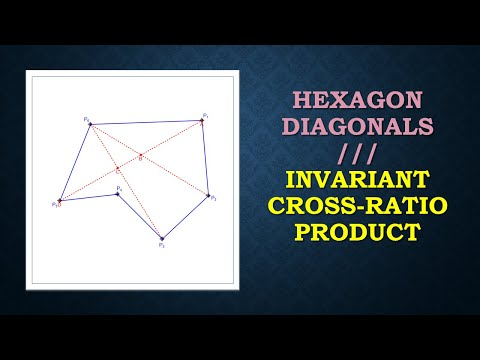
\includegraphics[width=.5\textwidth]{pics/heiqfRTQ2Mc.jpg}\end{center}
% Take any 6 points on the plane P1,...P6, and define 3 diagonals cyclically:

d1=(P1,P3), d2=(P1,P4), d3=(P2,P6).

Let A,B,C,D denote P2, intersect(d1,d3), intersect(d2,d3), and P6, respectively.

Claim, the cyclic product of cross ratios [AC;BD], for i=1,...6 is independent of the Pi and equal to 1.

Note: this property works for any even-sided polygon, with N greater than 5 (to be shown in upcoming video).

You can try this interactively at: http://bit.ly/3q2dLON
\end{enumerate}

\section{Early Results (8)}

\begin{enumerate}[resume]
\item \textbf{Mittenpunkt is stationary at center of billiard} (3m13s), 6/2019. \href{https://youtu.be/tMrBqfRBYik}{\url{youtu.be/tMrBqfRBYik}}
\begin{center}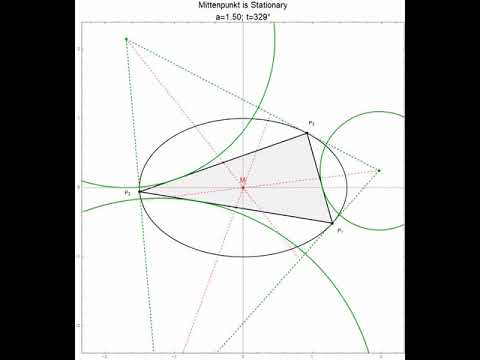
\includegraphics[width=.5\textwidth]{pics/tMrBqfRBYik.jpg}\end{center}
% The family of N=3 (triangular) orbits is shown in an elliptic billiard with a/b=1.5. The mittenpunkt X(9) of a triangle is the point of concurrence of lines drawn from each excenter through the corresponding side's median. For all orbits these are stationary at the origin.

More info: https://dan-reznik.github.io/Elliptical-Billiards-Triangular-Orbits/
\item \textbf{Stationary Circle for N=5} (2m25s), 7/2019. \href{https://youtu.be/dINE4aH1cvk}{\url{youtu.be/dINE4aH1cvk}}
\begin{center}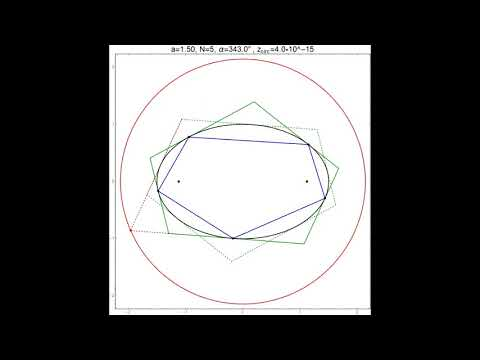
\includegraphics[width=.5\textwidth]{pics/dINE4aH1cvk.jpg}\end{center}
% An a/b=1.5 elliptic billiard is shown (black) as well as its family of N=5 (pentagonal) non-intersecting orbits (blue). Also shown is the orbits' excentral (exterior) polygon P' (solid green) and P'', the latter's reflection about the center of the billiard (dashed green). It turns out if, for any N odd, the locus of intersection of the ith edge of P' with the jth edge of P'', j=(N-1)/2, is circular.

We call this stationary circle the Monge-Darboux Circle in homage to the great French Geometers Gaspard Monge (1746-1818) and Jean-Gaston Darboux (1842-1917) which studied closely related geometries (Monge's Orthoptic Circle and the Poncelet-Darboux Grid of edge-edge intersection loci).

More Info: https://dan-reznik.github.io/Elliptical-Billiards-Triangular-Orbits/
\item \textbf{Stationary Circles} (2m25s), 7/2019. \href{https://youtu.be/EFeINGIDFrg}{\url{youtu.be/EFeINGIDFrg}}
\begin{center}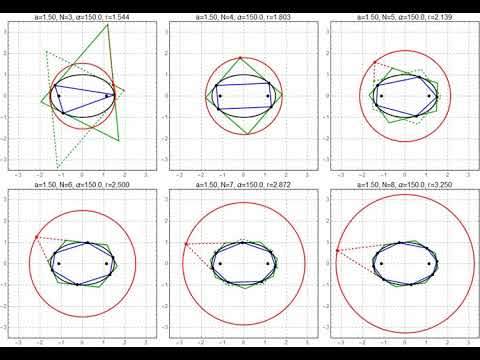
\includegraphics[width=.5\textwidth]{pics/EFeINGIDFrg.jpg}\end{center}
% Six a/b=1.5 elliptic billiards are shown (black), drawn to the same scale. Each billiard is shown with its family of N=3,4,....8, non-intersecting orbits (blue).

Also shown are T' the orbits' excentral (tangential) polygons (solid green). It turns out the intersection of segment (i,i+1) in T' with the reflection of segment (i+1,i+2) about the origin sweeps out circular loci (red). 

Because of the relationship with to Monge's Orthoptic Circles and the Poncelet-Darboux "grid" of loci of edge-edge intersections, we call these stationary objects Monge-Darboux Circles in homage to the great French Mathematicians Gaspard Monge (1746–1818), and Jean-Gaston Darboux (1842-1917).

More Info: https://dan-reznik.github.io/Elliptical-Billiards-Triangular-Orbits/
\item \textbf{Feuerbach Point Sweeps Billiard and its Anti-Complement and Extouch Points sweep caustic} (4m49s), 7/2019. \href{https://youtu.be/TXdg7tUl8lc}{\url{youtu.be/TXdg7tUl8lc}}
\begin{center}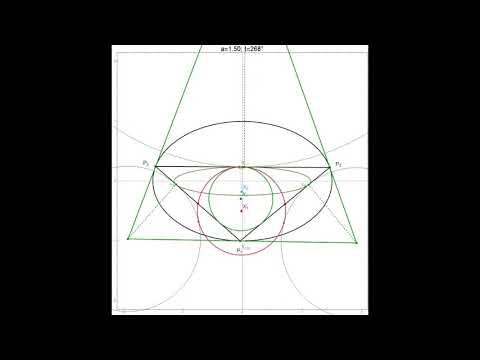
\includegraphics[width=.5\textwidth]{pics/TXdg7tUl8lc.jpg}\end{center}
% a/b=1.5 elliptic billiard shown as well as its family of N=3 orbits. Also shown are the X(1)-centered incircle (green), X(5)-centered nine-point circle (pink), and their point of contact, the Feuerbach point X(11). Also shown the X(100), the anticomplement of X(11), i.e., the Feuerbach point of the orbit's anticomplementary triangle. Equivalently, twice the reflection of X(11) about X(2). Not shown: X(9) lies stationary at the center of the billiard!

More Info:  https://dan-reznik.github.io/Elliptical-Billiards-Triangular-Orbits/
\item \textbf{Loci of Vertices of Medial, Intouch and Feuerbach Triangles is not elliptic} (4m49s), 7/2019. \href{https://youtu.be/OGvCQbYqJyI}{\url{youtu.be/OGvCQbYqJyI}}
\begin{center}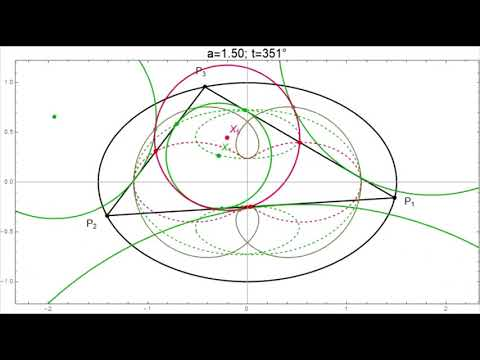
\includegraphics[width=.5\textwidth]{pics/OGvCQbYqJyI.jpg}\end{center}
% An a/b=1.5 elliptic billiard is shown with its family of N=3 (triangular) orbits. Also shown are the non-elliptic loci of the medians, the intouch points, and the external feuerbach points.

More information: https://dan-reznik.github.io/Elliptical-Billiards-Triangular-Orbits/
Interactive Applet: https://editor.p5js.org/dreznik/full/i1Lin7lt7
\item \textbf{Conservation of Sum and Product of Cosines} (3m13s), 7/2019. \href{https://youtu.be/P8ykpE_ZbZ8}{\url{youtu.be/P8ykpE\_ZbZ8}}
\begin{center}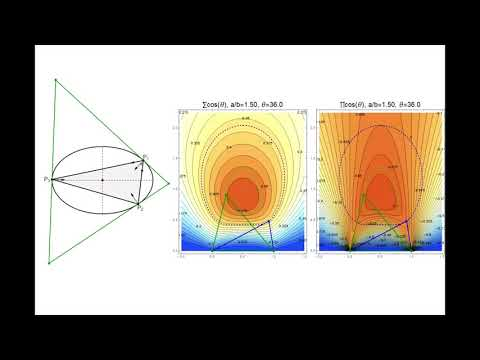
\includegraphics[width=.5\textwidth]{pics/P8ykpE_ZbZ8.jpg}\end{center}
% The 1d family of 3-periodics in an Elliptic Billiard not only has a stationary Mittenpukt X(9), but it also conserves an incredible quantity: r/R, the ratio of inradius-to-circumradius. Conservation corollaries include: (i) the sum of orbit's cosines = 1+r/R; (ii) the product of excentral cosines = r/(4R); and (iii) the ratio of excentral-to-orbit areas = r/(2R). Here we visualize (i) and (ii).

LEFT: An a/b=1.5 elliptic biliard is shown as well as its N=3 family of orbits (blue). For each orbit the excentral polygon is also shown (green). The red dot at the center of the billiard represents the stationary Mittenpunkt X(9). 

MIDDLE: a 2d representation of both orbit and excentral polygons is shown: a first vertex is placed at (0,0), a second one at (1,0), and a third one at some (u,v) location on the plane such that this normalized triangle is similar to the orbit (blue) or excentral (green). Drawn in the background are level curves of r/R for such a (u,v) family of triangles. Notice the (u,v) tip of the orbit triangle follows a constant r/R level-curve, whereas the excentral one does not. Note r/R=1+cosA+cosB+cosC, i.e., r/R level curves are congruent to sum-of-cosine ones.

RIGHT: the same as LEFT except level curves are shown for the *product* of cosines. Notice the excentral arm follows a product level curve perfectly whereas the orbit one does not.

In summary, orbit triangles conserve the *sum* of their cosines whereas the excentrals conserve the *product* of their cosines.

More Info:  https://dan-reznik.github.io/Elliptical-Billiards-Triangular-Orbits/
\item \textbf{Elliptic Loci of $X_{1}$ to $X_{5}$ and Euler Line} (4m49s), 7/2019. \href{https://youtu.be/sMcNzcYaqtg}{\url{youtu.be/sMcNzcYaqtg}}
\begin{center}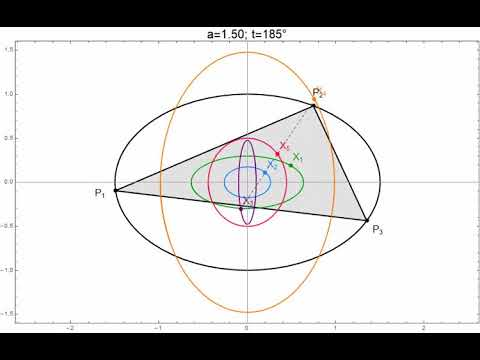
\includegraphics[width=.5\textwidth]{pics/sMcNzcYaqtg.jpg}\end{center}
% An a/b=1.5 elliptic billiard and its family of N=3 orbits is show, as well as the elliptic loci of the orbits' incenter, barycenter, circumcenter, orthocenter, and nine-point center. ALso shown is the Euler Line connecting all but the incenter.

More information: https://dan-reznik.github.io/Elliptical-Billiards-Triangular-Orbits/
Interactive Applet: https://editor.p5js.org/dreznik/full/i1Lin7lt7
\item \textbf{Generalization of the Stationary Mittenpunkt and Caustic-Sweeping Extouchpoints} (1m37s), 9/2019. \href{https://youtu.be/Bpc-MrR2IMc}{\url{youtu.be/Bpc-MrR2IMc}}
\begin{center}\includegraphics[width=.5\textwidth]{pics/Bpc-MrR2IMc.jpg}\end{center}
% N=4 and N=5 orbit families are shown in two Elliptic Billiards with a/b=1.5. Their Tangential Polygon is shown (green). whose vertices are intersections of tangents to consecutive orbit's vertices.  Two phenomena are illustrated:

1) Generalized N=3 Mittenpunkt: (dashed red) lines drawn from each Tangential vertex through the corresponding sides' midpoints all concur at the Billiard Center

2) Generalized N=3 Extouchpoints: the feet of (dashed green) perpendiculars dropped from each tangential vertex to the corresponding side is congruent with the point of tangency of that side with the confocal caustic, i.e., the locus of these feet is the caustic.

More info: https://dan-reznik.github.io/Elliptical-Billiards-Triangular-Orbits/
\end{enumerate}

\section{Ellipse-Inscribed Triangles (8)}

\begin{enumerate}[resume]
\item \textbf{Ellipse-Mounted Triangles: Elliptic locus of the Orthocenter $X_{4}$ and suprising area invariance!} (9m17s), 7/2020. \href{https://youtu.be/Fo-tNRcA-CQ}{\url{youtu.be/Fo-tNRcA-CQ}}
\begin{center}\includegraphics[width=.5\textwidth]{pics/Fo-tNRcA-CQ.jpg}\end{center}
% Consider an ellipse with semi-axes a,b. Choose two fixed points on it:

v1 = [a cos(t1), b sin(t1)]
v2 = [a cos(t2), b sin(t2)]

Let a third point P(t) ride on the ellipse, and let T be the triangle {v1,v2,P(t)}. Observations:

a) the locus of the orthocenter X4 of T is *always* an upright ellipse (axis aligned with the original one, but with major axis vertical and minor horizontal).

b) pick an angle "k". over all v1,v2 such that t1+t2=k, the locus generated is the same ellipse up to translation!

c) the maximal (resp minimal) area elliptic locus occurs for k = 180 (resp. 0) degrees.

to do:

- where is the center of the elliptic locus
- what are its axes
- what is its translation (looks like a straight line) as one visits all t1+t2=k?

Having fun folks!
\item \textbf{Circle-Mounted Triangles: Surprising Loci of the Brocard Points} (2m47s), 7/2020. \href{https://youtu.be/Ms8jC9yOKU4}{\url{youtu.be/Ms8jC9yOKU4}}
\begin{center}\includegraphics[width=.5\textwidth]{pics/Ms8jC9yOKU4.jpg}\end{center}
% This video explores the loci of the two Brocard points [1] for a family of triangles with two stationary vertices on the circumference of a circle and a third one free to revolve around the same circle.

Indeed a few experimental suprises were in store!
\item \textbf{Loci of Ellipse-Inscribed Triangles I: Basic Phenomena} (3m3s), 10/2020. \href{https://youtu.be/zjiNgfndBWg}{\url{youtu.be/zjiNgfndBWg}}
\begin{center}\includegraphics[width=.5\textwidth]{pics/zjiNgfndBWg.jpg}\end{center}
% A triangle V1 V2 P(t) (blue) is inscribed in an ellipse E (black) with semi-axes a,b (in the video a/b=1.5). While V1,V2 are fixed, P(t) slides along E's boundary. Show are the loci of the barycenter X2 (brown), circumcenter X3 (red), orthocenter X4 (orange), collinear on the Euler line (dashed green). 

As it turns out, for any choice of fixed V1,V2, the locus of:

- X2 is an ellipse axis-aligned w E, with semi-axes a/3,b/3
- X3 is a segment
- Z4 is an ellipse axis-aligned w E, with aspect ratio equal to a/b.

An intermediate point X(ρ)=X2+ρ(X4-X2) is shown which is a fixed linear combination of X2 and X4 (in the video ρ=0.5, which makes X(ρ) be X381 [1]). For whichever choice of V1,V2 and ρ, the locus of X(ρ) is always an ellipse (green), in general not axis-aligned w E.

[1] C. Kimberling, "Encycl. of Triangle Centers", 2020. https://faculty.evansville.edu/ck6/encyclopedia/ETC.html
\item \textbf{Loci of Ellipse-Inscribed Triangles II: $X_\rho$ slides merrily along the Euler line} (2m12s), 10/2020. \href{https://youtu.be/w5KuN_0rQBQ}{\url{youtu.be/w5KuN\_0rQBQ}}
\begin{center}\includegraphics[width=.5\textwidth]{pics/w5KuN_0rQBQ.jpg}\end{center}
% A triangle V1 V2 P(t) (blue) is inscribed in an ellipse E (black) with semi-axes a,b (in the video a/b=1.5). While V1,V2 are fixed, P(t) slides along E's boundary. Show are the elliptic loci of the barycenter X2 (brown), circumcenter X3 (red), orthocenter X4 (orange), collinear on the Euler line (dashed green) and of an point X(ρ)=X2+ρ(X4-X2) on the Euler line for variable ρ. 

As ρ varies, the locus of X(ρ) is a family of ellipse (in general not axis-aligned w E) whose center Oρ follows a straight line (dashed purple). Notice at ρ=-1/2 (at X3), and also at some second location, one of the axes of said locus vanishes.

[1] C. Kimberling, "Encycl. of Triangle Centers", 2020. https://faculty.evansville.edu/ck6/encyclopedia/ETC.html
\item \textbf{Loci of Ellipse-Inscribed Triangles III: family of V1V2 parallels causes rigid locus translation} (2m48s), 10/2020. \href{https://youtu.be/zFOeENDJRho}{\url{youtu.be/zFOeENDJRho}}
\begin{center}\includegraphics[width=.5\textwidth]{pics/zFOeENDJRho.jpg}\end{center}
% Consider the family of triangles T(t)=V1V2P(t) inscribed in an ellipse E with axes a,b. Namely, V1,V2 are fixed on the boundary of E and P(t) executes one revolution along it.

The video shows the loci of triangle centers X2,X3,X4,X5 of T(t) [1] which are all ellipses (except X3 which is a segment). Specifically, we can observe how these loci change over parallel V1V2 (P(t) is not shown).

What is observed is that as V1V2 is translated, the loci also translate. Interestingly, the motion of their center is a line (magenta) which passes thru the center of E.

[1] C. Kimberling, "Encycl. of Triangle Centers", 2020. https://faculty.evansville.edu/ck6/encyclopedia/ETC.html
\item \textbf{Loci of Ellipse-Inscribed Triangles IV: Multiple Loci Over Parallel V1V2} (1m46s), 10/2020. \href{https://youtu.be/TpBjKlkFjkg}{\url{youtu.be/TpBjKlkFjkg}}
\begin{center}\includegraphics[width=.5\textwidth]{pics/TpBjKlkFjkg.jpg}\end{center}
% Consider the family of triangles T(t)=V1V2P(t) inscribed in an ellipse E with axes a,b. Namely, V1,V2 are fixed on the boundary of E and P(t), not shown, executes one revolution along it.

It turns out that provided a point X lies on the Euler line at some fixed linear combination of X2 and X4, its locus will be an ellipse over T(t). The video shows elliptic loci for triangle centers X2,X5,X381,X4.

Furthermore:

1) Over the family of parallel V1V2, said loci rigidly translate
2) For a given V1V2, the center of all loci are collinear.
3) When V1 and V2 are symmetric about the center of E, the centers of all loci collapse to a point.

In the video one can observe how the discrete family of loci change their relative position as a family of parallel V1V2 is traversed.
\item \textbf{Loci of Ellipse-Inscribed Triangles V: Circular Loci if V1V2 Horizontal or Vertical for Certain $\rho$} (2m49s), 10/2020. \href{https://youtu.be/nLeKvxcicNY}{\url{youtu.be/nLeKvxcicNY}}
\begin{center}\includegraphics[width=.5\textwidth]{pics/nLeKvxcicNY.jpg}\end{center}
% Consider the family of triangles T(t)=V1V2P(t) inscribed in an ellipse E with axes a,b. Namely, V1,V2 are fixed on the boundary of E and P(t), not shown, executes one revolution along it. Consider the locus of a a point X a fixed linear combination of the barycenter X2 and orthocenter X4, i.e.:

X = X2 + (X4-X2) ρ

The video shows an intriguing result: only if V1V2 is either horizontal or vertical can said locus be a circles. Specifically, two values of ρ for each configuration accomplish this.
\item \textbf{Ellipse-Inscribed Triangles VI: Envelope of $X_{4}$ Loci is Area-Invariant and Cousin of Pascal's Limaçon} (3m5s), 10/2020. \href{https://youtu.be/sPQrz7ddRfA}{\url{youtu.be/sPQrz7ddRfA}}
\begin{center}\includegraphics[width=.5\textwidth]{pics/sPQrz7ddRfA.jpg}\end{center}
% Consider the triangle family T(t)=V1V2P(t) inscribed in an ellipse E (black) of semiaxes a,b. Let V1 and V2 be fixed on E while P(t) executes one revolution on it.

1) Let X be a triangle center. Over the T(t), the locus of X will be an ellipse if X is a fixed linear combination of the barycenter X2 and orthocenter X4. (X will necessarily lie on the Euler Line).

2) Consider the case where X=X4. In this case, it can be shown that for any choice of V1,V2, the locus is an upright ellipse passing thru said points, which is axis-aligned with E and has aspect ratio of b/a.

3) Now pick a V1. Over all possible (fixed) placements of V2, one obtains a family of elliptic loci w the features in (2). It can be shown their centers will lie on an ellipse (red) whose aspect ratio is also a/b.  The *envelope* of said family will be a (generally) non-convex shape (pink), which is the affine image of Pascal's Limaçon [1].

The video shows said locus family as one varies V1, as well as the locus of their centers (an red ellipse) and their varying envelope (pink). Surpringly, the envelope is area-invariant over all V1, and this is valid for any triangle center X.

Note: the origin of the term "Limaçon" is the latin for snail, "limax".

[1] E. Weisstein, "Pascal's Limaçon", Mathworld, 2020. https://mathworld.wolfram.com/Limacon.html
\end{enumerate}

\section{Ellipse Echoes (1)}

\begin{enumerate}[resume]
\item \textbf{Ellipse Echoes I: Circular wavefronts released into circular and elliptic cavities} (12m27s), 1/2021. \href{https://youtu.be/LQnNLMhH9EE}{\url{youtu.be/LQnNLMhH9EE}}
\begin{center}\includegraphics[width=.5\textwidth]{pics/LQnNLMhH9EE.jpg}\end{center}
% These are early experiments with the geometry of circular wavefronts released from a boundary or interior point of a circular or elliptic cavity.

These can be tried at: https://dan-reznik.github.io/ellipse-echo-p5js/
\end{enumerate}

\section{Envelopes (9)}

\begin{enumerate}[resume]
\item \textbf{Envelope of Antiorthic and Gergonne Lines} (2m43s), 2/2020. \href{https://youtu.be/Q7l6_Z4IyEI}{\url{youtu.be/Q7l6\_Z4IyEI}}
\begin{center}\includegraphics[width=.5\textwidth]{pics/Q7l6_Z4IyEI.jpg}\end{center}
% The isogonal (or isotomic) conjugate of a line with respect to a triangle is a circumconic [1].

If an elliptic billiard is regarded as a stationary, X(9)-centered circumellipse to the 3-periodic family, we can analyze its isogonal and isotomic conjugate lines dynamically. These turn out to be [3] the orbits' Antiorthic Axis [4] and Line L(31) [5], respectively.

In particular, what is the envelope [2] of such straight lines over the family of 3-periodics?

The two lines can be constructed with any pair of Triangle Centers lying on them (Peter Moses provides many in [3]). For special reasons, we use:

a) L(1), Antiorthic Axis, X(44)X(513)
b) L(31), Line X(514)X(661) -- note: to be reviewed, but this is the Gergonne line of a triangle derived from the reference one. ACT?

The video shows the locus of the above Triangle Centers for an a/b=1.618=phi billiard, drawn black. Orbits are drawn blue, as well as the envelope of said lines.

Specifically:

Left: the non-elliptic locus of X(44) is shown red. The elliptic locus of X(1155) is shown green. Notice how the Antiorthic axis (dashed blue) is dynamically tangent to the latter, i.e., the locus of X(1155) is the envelope of the Antiorthic Axis.

Right: the non-elliptic locus of X(857) which lies on L(31) is shown red. The elliptic locus of X(908), also on L(31), is shown green. Notice how line L(31) (dashed blue) is dynamically tangent to the latter, i.e., the locus of X(908) is the envelop of L(31).

In both cases, "C" depicts where the envelope currently is.

[1] http://mathworld.wolfram.com/Circumconic.html
[2] http://mathworld.wolfram.com/Envelope.html
[3] Peter Moses, mentioed by Clark Kimberling, ETC under X(9), https://faculty.evansville.edu/ck6/encyclopedia/ETC.html
[4] http://mathworld.wolfram.com/AntiorthicAxis.html
[5] https://faculty.evansville.edu/ck6/encyclopedia/CentralLines.html
\item \textbf{Evolute of Elliptic Billiard and Envelope of $X_{1}$-$X_{5}$} (4m1s), 2/2020. \href{https://youtu.be/eBStp-7X5yE}{\url{youtu.be/eBStp-7X5yE}}
\begin{center}\includegraphics[width=.5\textwidth]{pics/eBStp-7X5yE.jpg}\end{center}
% The envelope to a family of lines is that curve to which every member is tangent, aka as the Caustic [1]. We are intersested in the envelopes generated by pairs of Triangle Centers over the 3-periodic family.

An a/b=1.618 elliptic billiard (EB) is shown (black) as well as its family of 3-periodics (triangular orbits, blue).

Also shown are X1 and X5 riding along their elliptic loci (red, green, respectively). The X1X5 line is shown purple. Its envelope (purple) is the 4-cuspid astroidal curve. Miraculously, this is simultaneously tangent to the X1 and X5 locus! Any idea how?

Also shown is the evolute [2] of the elliptic billiard,which is the envelope of inward-pointing normals. This is also astroidal and shown dashed blue.  This curve has a pleasant closed-form parametric expression in terms of a,b the ellipse's axes [2]:

x(t) = (a^2-b^2) cos(t)^3 / a
y(t) = (b^2-a^2) sin(t)^3 / b

Let P1(t) be a vertex of a 3-periodic. The line P1X1 is parallel to the ellipse normal at P1, therefore this family yields the involute.

The instantaneous X1X5 line is shown purple having the purple envelope as its caustics. The instantaneous P1X1 line is drawn gray, and its caustic is the ellipse evolute.

Suprisingly both the evolute and the X1X5 caustic touch the X1 locus on the same four spots (marked by blue dots). One of them is given by:

x1= c2 ((-b2 + d)/c2)^(3/2)/a
y1 = c2 ((a^2 - d)/c2)^(3/2)/b

where  a2=a*a, b2=b*b, d = Sqrt[a2^2 - a2*b2 + b2^2], and c2=a2-b2

The Orthocenter X4 is shown as an orange dot. When it is on one of the 3-periodic vertices, the 3-periodic is a right triangle. There doesn't seem to be any specific phenomena tied to such configurations.

A large gallery of Triangle Center pairs and their envelopes is available in [3].

[1] http://mathworld.wolfram.com/Envelope.html
[2] http://mathworld.wolfram.com/EllipseEvolute.html
[3] https://dan-reznik.github.io/Elliptical-Billiards-Triangular-Orbits/envelopes1618.html
\item \textbf{Envelope of 3-Periodic Vertex with Triangle Center} (2m41s), 2/2020. \href{https://youtu.be/bRY61RdxCkM}{\url{youtu.be/bRY61RdxCkM}}
\begin{center}\includegraphics[width=.5\textwidth]{pics/bRY61RdxCkM.jpg}\end{center}
% Consider the family of 3-periodics in an Elliptic Billiard with axes a,b [1]. Let each triangular 3-periodic be defined by vertices P1,P2,P3, where P1(t) = [a cos(t), b sin(t)], t=[0,2π) is used as a parametrization. 

Take a Kimberling Center [2] Xi, and consider the family of lines defined by [P1(t),Xi(t)].

The video shows the envelope [3] of such a family for various Xi, i=1,2,3,4,5,6,7,8,10,11,12,20, over a/b=[1.,2).

Notable cases include:

a) P1X1: the evolute [4] of the billiard boundary. as these are always parallel to the normal at P1
b) P1X5: spiderman? why does it explote?

More info in [5].

Note: the lower right animation of X(20) is incorrectly showing X(12). To be corrected.

[1] https://dan-reznik.github.io/Elliptical-Billiards-Triangular-Orbits/videos.html
[2] https://faculty.evansville.edu/ck6/encyclopedia/ETC.html
[3] http://mathworld.wolfram.com/Envelope.html
[4] http://mathworld.wolfram.com/Evolute.html
[5] https://dan-reznik.github.io/Elliptical-Billiards-Triangular-Orbits/envelopes1618.html
\item \textbf{Evolute Triangles of P1(t) with $X_i$} (8m1s), 2/2020. \href{https://youtu.be/DhqDdMAlBZM}{\url{youtu.be/DhqDdMAlBZM}}
\begin{center}\includegraphics[width=.5\textwidth]{pics/DhqDdMAlBZM.jpg}\end{center}
% Given a 3-periodic T=Pi, i=1,2,3, elliptic billiard w axes a,b. Let P1(t) = [a cos(t), b sin(t) ], and X be a Triangle Center of T. Explicit expressions for P2(t) and P3(t) can be found here [1].

We define the "Evolute Triangle" of (T,Xi) by the instantaenous tangency points of P1(t)X_i, P2(t)X_i, P3(t)X_i to their common envelope [2]. These are shown in pink for i=1,3,5,20, for an a/b=1.45. We've found that for higher a/b some of the envelopes become too large and/or non-compact.

Note: the envelope of (T,X1) is the evolute of the billiard [3].
 
[1] Ronaldo Garcia, "Elliptic Billiards and Ellipses Associated to the 3-Periodic Orbits", Am. Math. Monthly, Volume 126, 2019 - Issue 6
[2] http://mathworld.wolfram.com/Envelope.html
[3] http://mathworld.wolfram.com/EllipseEvolute.html
\item \textbf{Elliptic Envelope of P1(t) with P1(t+$\pi/2$)} (3m13s), 3/2020. \href{https://youtu.be/8a4JoddyEyc}{\url{youtu.be/8a4JoddyEyc}}
\begin{center}\includegraphics[width=.5\textwidth]{pics/8a4JoddyEyc.jpg}\end{center}
% Let a vertex P1 of a 3-periodic in en Elliptic Billiard (black) be parametrized as P1=[a cos(t), b sin(t)], and its copy P1', lying 90 degrees ahead as: P1'=[a cos(t+pi/2), b sin(t+pi/2)] = [a sin(t), - b cos(t)]. The 3-periodic initiating at P1 (resp. P1') is shown blue (resp. dashed blue).

The video shows the family of lines [P1,P1'] (red) and the caustic they envelope (green): an ellipse similar to the EB itself. The tangency point "C" is dynamically the midpoint between P1 and P1'.

The above can be proven via an affine transformation which takes the EB to a circle (multiply the x coordinate by b/a). In this new ambient, the billiard is a circle, and the 3-periodic and its forward doppleganger are equilaterals, and the internal caustic is the common incircle. By symmetry, these equilaterals will be tangent to the incircle at their midpoints. At the original space, the caustic is the inverse affine transform of the incircle.
\item \textbf{Envelope of 3-Periodic P1 and reflected P2 is Elliptic} (6m1s), 3/2020. \href{https://youtu.be/GJgiUulX1aU}{\url{youtu.be/GJgiUulX1aU}}
\begin{center}\includegraphics[width=.5\textwidth]{pics/GJgiUulX1aU.jpg}\end{center}
% An a/b=1.5 Elliptic Billiard is shown as well as its family of  3-periodics (blue) and their caustic (brown). A copy of the latter (reflected about the Billiard Center) is also shown (dashed blue). The [P1, -P2] family of lines (red) is instantaneous tangent (at "C") to a non-confocal elliptic caustic (green). Note [P1,-P2] is vertical/horizontal at when the 3-periodics are isosceles, suggesting a simple method to compute the axis of the (green) caustic.
\item \textbf{The Bat-Envelope of $X_{48}$ and $X_{37143}$} (1m21s), 3/2020. \href{https://youtu.be/Kr93eFZnB_U}{\url{youtu.be/Kr93eFZnB\_U}}
\begin{center}\includegraphics[width=.5\textwidth]{pics/Kr93eFZnB_U.jpg}\end{center}
% An elliptic billiard (EB) is shown with aspect ratio a/b=1.618...=golden ratio. Also shown is its family of 3-periodics (blue triangles). Also shown are Triangle Centers [1] X(48) and X(37143) [formerly the isotomic conjugate of X(30565)]. The former's locus is an upright convex curve (green, not a proper ellipse [3]), whereas the latter rides along the EB (it is a "swan" [4]). Also shown is the envelope [2] (purple) of the family of lines defined by the pair. Holy Mackerel, this looks like a sideways bat!

For the aspect ratio a/b=golden ratio chosen, we do not understand why:

(i) both centers move monotonically with respect to the 3-periodic family;
(ii) the envelope has 8 tangency points with the locus of X(48); 
(iii) when "C" passes thru these so does X(48). why?
(iv) four tangency points intersect the Elliptic Billiard precisely where the (non-elliptic) locus of X(48) intersects it;
(v) there are 8 cusps;
(vi) two of which coincide with the billiard's foci;
(vii) what kind of curves are those between the cusps? could they be elliptic arcs?

For additional harmonies when "C" lies at the cusps and/or tangency points of the envelope with X(48), visit [5].

[1] https://faculty.evansville.edu/ck6/encyclopedia/ETC.html
[2] https://mathworld.wolfram.com/Envelope.html
[3] https://arxiv.org/abs/2001.08041
[4] https://arxiv.org/abs/2002.00001
[5] https://dan-reznik.github.io/Elliptical-Billiards-Triangular-Orbits/envelopes1618.html
\item \textbf{Envelopes of Sides of Derived Triangles} (2m1s), 3/2020. \href{https://youtu.be/SJrgWtdX8xU}{\url{youtu.be/SJrgWtdX8xU}}
\begin{center}\includegraphics[width=.5\textwidth]{pics/SJrgWtdX8xU.jpg}\end{center}
% Consider the family of 3-periodics in an Elliptic Billiard with aspect ratio a/b. The envelope of its sides is a confocal caustic. The video shows the envelope of the sides 16 well-known derived triangles, as the aspect ratio is varied. Equivalently, shown is the envelope of the line family defined by two consecutive vertices of a derived triangle.
\item \textbf{Envelope of Simson Lines from $X_{100}$ and $X_{99}$ to two N=3 Poncelet Families} (4m5s), 6/2020. \href{https://youtu.be/79veSHrElb4}{\url{youtu.be/79veSHrElb4}}
\begin{center}\includegraphics[width=.5\textwidth]{pics/79veSHrElb4.jpg}\end{center}
% Both ellipses shown have a/b=1.5.

Left: 3-periodics (blue) in the Elliptic Billiard (EB, black). Recall these have stationary Mittenpunkt X9, and that X100 lies at the intersection of the circumcircle with the X9-centered circumellipse, i.e., the EB. Over the family of 3-periodics, the envelope of Simson lines (red) with respect o X100 is an astroid-like curve (purple). The envelope of lines (dashed red) passing through X100 and perpendicular to the aforementioned Simson family is a "cushion shaped" curve (purple) w four cusps, tangent to the EB at the four vertices. Also shown is the EB's evolute (dashed black).

Right: the N=3 poncelet family (blue) inscribed in their Steiner Ellipse (a,b) semiaxes and centered on X2, with the Steiner Inellipse (a/b,b/2) as their caustic has constant area. Recall X99 lies at the intersection of the Steiner Ellipse with the Circumcircle. Over this family, the envelope of Simson lines (red) with respect o X100 is also an astroid-like curve (purple). The envelope of lines (dashed red) passing through X99 and perpendicular to the aforementioned Simson family is also a "cushion shaped" curve (purple) w four cusps, tangent to the EB at the four vertices. Also shown is the EB's evolute (dashed black).
\end{enumerate}

\section{Frégier (3)}

\begin{enumerate}[resume]
\item \textbf{Frégier Phenomena I: Area-Invariant Envelope of Chords} (16m15s), 1/2021. \href{https://youtu.be/UCCG5AT8dh8}{\url{youtu.be/UCCG5AT8dh8}}
\begin{center}\includegraphics[width=.5\textwidth]{pics/UCCG5AT8dh8.jpg}\end{center}
% This is joint work with M. Helman, R. Garcia, and D. Laurain, who introduced us to M. Frégier's wonderful theorem [1,2].

In 1810 M. Frégier (French Mathematician) discovered a remarkable fact. Take a point M on an ellipse E and consider all pairs of rays at a right angle with each other emanating from M. Consider the family of chords defined by the intersections of these rays with E. All such chords pass thru a common point F, called the "Frégier Point" [2].

Let ϴ denote the angle between the pairs of rays, above ϴ=90 degreess. The video shows the following old/new facts:

a) Probably known: the locus of F over all M is an ellipse.

Let ϴ denote the angle between the pair of rays. When ϴ is not 90, the following observations could be new:

b) the family of chords envelops an ellipse E', which is in general non-concentric and not axis-aligned with E.
c) Over all M, the semi-axes of E' are variable as is their ratio.
d) Remarkably, the *area* of E' is invariant over M!!!
e) Over all M, the centers of E' span a 3rd ellipse, E'', this time concentric, axis-aligned and *homothetic* to E.

The video also shows a "real-time" discovery: when ϴ=60, the envelope of chords in [b] will be inscribed in the triangle formed by M, and the two rays emitted symmetrically from the normal (at 30 and -30 degrees) and the chord between the intersections.

Any help w/ proofs appreciated!

[1] D. Laurain, Private Communication, Jan 2021. 
[2] E. Weisstein, "Frégier's Theorem", MathWorld, 2020. https://mathworld.wolfram.com/FregiersTheorem.html
\item \textbf{Frégier Phenomena II: Envelope of Chords over M} (11m50s), 1/2021. \href{https://youtu.be/mJ6opTPFAO4}{\url{youtu.be/mJ6opTPFAO4}}
\begin{center}\includegraphics[width=.5\textwidth]{pics/mJ6opTPFAO4.jpg}\end{center}
% This is a continuation of the previous video.

Let M be a point on the boundary of an ellipse E. Let n be the ellipse normal at M.  Let Q1 and Q2 be the intersections of tow rays shot from M, along rays r1 and r2 (blue in the video), which are copies of n rotated by β+α and β-α. 

Before we sawo that when α=90, for fixed M, and over all β, the envelope of Q1Q2 is a point, known as the Frégier point [2]

The video shows the envelope of Q1Q2 for various combinations of fixed α,β, but over all M on E. These can contain cusps, stationary points, or be regular.
\item \textbf{Frégier Phenomena III: Circular Envelopes and a New Invariant for a Poncelet Family} (18m11s), 1/2021. \href{https://youtu.be/AzNXeBU2NTI}{\url{youtu.be/AzNXeBU2NTI}}
\begin{center}\includegraphics[width=.5\textwidth]{pics/AzNXeBU2NTI.jpg}\end{center}
% We observe the dynamic geometry of elliptic envelopes over 4 different Poncelet families and discover a neat invariant. Let me know if you have ideas on how to prove it.
\end{enumerate}

\section{Harmonic Polygons (6)}

\begin{enumerate}[resume]
\item \textbf{Inversive-Area Iso-Contours of Harmonic Polygons (obtained as Polar Images of the Homothetic family)} (2m26s), 8/2021. \href{https://youtu.be/erV4NILgWrE}{\url{youtu.be/erV4NILgWrE}}
\begin{center}\includegraphics[width=.5\textwidth]{pics/erV4NILgWrE.jpg}\end{center}
% A family (blue) of triangles (left) and quadrilaterals (right) are shown which are Poncelet families interscribed in a pair of homothetic ellipses (only the outer one is shown). These can also be regarded as affine images of a family of regular polygons.

Also shown are their polar images (magenta) with respect to the left focus of the caustic (not shown). These are  inscribed in a (dashed magenta circle) and circumscribe a Brocard inellipse (not shown). Their Brocard points lie at the foci of the latter. This class of polygons is known as "harmonic" since they can also be regarded as the image of regular polygons under inversion [1,2,3].

The animation shows isocurves of are of the inversion of the harmonic family wrt to point on the plane, as they revolve.

[1] J. Casey, "A sequel to the first six books of the Elements of Euclid", Longman, Dublin, 1888

[2] T. Sharp, "Harmonic Polygons", The Mathematical Gazette
Vol. 29, No. 287 (Dec., 1945), pp. 210-213.

[3] A. Zazlavsky and A. Akopyan, "Геометрические свойства кривых
второго порядка" (Geometric properties of curves of second order), sec. 4.6, pp. 129. MCNMO Publishing House, Moscow, 2011.
\item \textbf{Inversive Image of Pivoting Harmonic Family Part I: Stationary Inversive Symmedian/Lemoine Point} (9m53s), 8/2021. \href{https://youtu.be/jn3GD9SEkdU}{\url{youtu.be/jn3GD9SEkdU}}
\begin{center}\includegraphics[width=.5\textwidth]{pics/jn3GD9SEkdU.jpg}\end{center}
% This is a generalization of results regarding triangles in previous videos.

A family of harmonic polygons H (magenta) is shown inscribed in a circle. John Casey (1888) constructs them as the inversive images of regular N-gons with respect to some circle [1]. T. Sharp (1945) constructs them as projections of a regular polygon [2].  Harmonic polygons have a symmedian point K. If N is even these are the intersections of diagonals. If N is odd these are the intersections of lines from the vertices to the opposite points of contact with the ellipse enveloped by the sides (aka the Brocard inellipse).

The video shows a few curious properties of the inversive image H' of harmonic polygons (unproved) wrt to an inversion circle C with center Cinv.

1) Trivially H' is also harmonic (the composition of two inversions is an inversion).
2) The symmedian K' of H' is stationary and collinear with Cinv and K.
3) Amazingly, over rigid rotations of H about K, K' is stationary!
symmedian inversive image of the harmonic family wrt fo a fixed circle is harmonic

[1] John Casey, "A sequel to the first six books of the Elements of Euclid, containing an easy introduction to modern geometry, with numerous examples". Dublin: Hodges, Figgis & co., 1888.
[2] T. Sharp, "Harmonic Polygons", The Mathematical Gazette, Vol. 29, No. 287 (Dec., 1945), pp. 210-213.
\item \textbf{Inversive Image of Pivoting Harmonic Family Part II: Rigid Rotations about Harmonic Limiting Points} (13m44s), 8/2021. \href{https://youtu.be/9GwfELl-tHk}{\url{youtu.be/9GwfELl-tHk}}
\begin{center}\includegraphics[width=.5\textwidth]{pics/9GwfELl-tHk.jpg}\end{center}
% A family of harmonic polygons H (magenta) is shown inscribed in a circle centered at O. John Casey (1888) constructs them as the inversive images of regular N-gons with respect to some circle [1]. T. Sharp (1945) constructs them as projections of a regular polygon [2].

Harmonic polygons have a symmedian point K. If N is even these are the intersections of diagonals. If N is odd these are the intersections of lines from the vertices to the opposite points of contact with the ellipse enveloped by the sides (aka the Brocard inellipse).

Define the Brocard circle as having KO as diameter. Let l1 and l2 be the limiting points of the pencil defined by the circumcircle and Brocard circle of a harmonic family. Consider a family H' (also harmonic) whose vertices are the inverses of those of H wrt to a circle centered somewhere.

The video shows that when a harmonic family is rotated about either limiting point l1 or l2, the corresponding limiting point of H' stays put.

[1] John Casey, "A sequel to the first six books of the Elements of Euclid, containing an easy introduction to modern geometry, with numerous examples". Dublin: Hodges, Figgis & co., 1888.
[2] T. Sharp, "Harmonic Polygons", The Mathematical Gazette, Vol. 29, No. 287 (Dec., 1945), pp. 210-213.
\item \textbf{Harmonic Polygons, Part III: Isocurves of Inversive Brocard Angle are Circles of the Schoute Pencil} (15m13s), 8/2021. \href{https://youtu.be/VFqSvpuU0wg}{\url{youtu.be/VFqSvpuU0wg}}
\begin{center}\includegraphics[width=.5\textwidth]{pics/VFqSvpuU0wg.jpg}\end{center}
% Let H (blue) be a harmonic polygon (blue) , and let H' (red) be a new polygon with vertices at the inversions of those of H wrt to a circle centered on a point C. H' is also harmonic [1, Section VI].

The video shows two potentially new observations which are likely generalizations of [3, Thm 11], to harmonic polygons.

a) the isocurves of Brocard angle of H' are circles in the pencil of the circumcircle and Brocard circle of H, also known as the Schoute pencil [2,3]. 
b) if C is on the Brocard circle or on the radical axis of the pencil, then the Brocard angle of H' is equal to that of H.

[1] J. Casey, "A Sequel to Euclid Elements", Longman, London, 1888.
[2] P. Pamfilos, "Symmedian", Geometrikon, http://users.math.uoc.gr/~pamfilos/eGallery/problems/Symmedian.pdf
[3] R. Johnson, "Directed Angles and Inversion, and a Proof of Schoute's Theorem", American Math. Monthly, 24:313–317, 1917.
\item \textbf{Harmonic Polygons, Part IV: Four Harmonic Inversive Images of Steiner's Porism} (2m26s), 9/2021. \href{https://youtu.be/PGaUZHOvQIg}{\url{youtu.be/PGaUZHOvQIg}}
\begin{center}\includegraphics[width=.5\textwidth]{pics/PGaUZHOvQIg.jpg}\end{center}
% Steiner's porism [1] consists of a chain of touching circles moving (as their radii vary) in the interstice between to non-concentric circles. They are the inversive image of a "ball bearing" with identical circular disks between two concentric circles. In [2,3] it was stated that 4 harmonic polygons can be built out of Steiner's porism. Deeper connections with invariant symmetric polynomials are are explored in [4].

Let ri be the radii of the disks in a Steiner porism. The video shows sum(1/ri), sum(1/ri^2), sum(1/ri^3) is conserved.

The centers of the original disks are the vertices of a regular polygon. Their inversive image with respect to C is a harmonic polygon (green).

Also harmonic are the polygons (magenta) with vertices at the inversions of points of contact of the bearings with (i) the inner circle, (ii) outer circle, and (iii) with each other.

All said 4 harmonic families are distinct, and each conserves a different sum of cotangents of internal angles (sums of cot^2 and cot^3 are also conserved).


[1] E. Weisstein, "Steiner's Porism", MathWorld 2021. https://mathworld.wolfram.com/SteinersPorism.html

[2] G. Tarry & J. Neuberg, "Sur les polygones et les polyèdres harmoniques", Comptes rendus de l'Association française pour l'avancement des sciences, 1887. Note: extrait du Congrès de Nancy, 1886.

[3] T. C. Simmons, "A new Method for the Investigation of Harmonic Polygons, Proc London Math. Soc., Volume 1--18, number 1, pp. 289--304, 1886.

[4] R. Schwartz & S. Tabachnikov, "Descartes Circle Theorem, Steiner Porism, and Spherical Designs", Am. Math. Monthly, volume 127, Issue 3, 2020.
\item \textbf{Exploring the Dynamic Geometry and Conservations of the Steiner-Soddy and Harmonic Poncelet Porims} (22m43s), 1/2022. \href{https://youtu.be/1zrp1HMeUbk}{\url{youtu.be/1zrp1HMeUbk}}
\begin{center}\includegraphics[width=.5\textwidth]{pics/1zrp1HMeUbk.jpg}\end{center}
% The video explores the dynamic geometry and conservations in a Poncelet porism whose vertices are the centers of circles in a Steiner chain with N circles. This family is the polar image of the harmonic family with respect to its circumcircle. One of the main observations is that the sum of tangents of half angles to the power of k, with k less than N is conserved. See [1,2,3].

References:

[1] Richard Schwartz and Sergei Tabachnikov,  "'Descartes Circle Theorem, Steiner Porism, and Spherical Designs", American Math Monthly Vol 127 Issue 3 (2020)
[2] Ronaldo Garcia, Dan Reznik, Pedro Roitman, "New Properties and Invariants of Harmonic Polygons", 2021. https://arxiv.org/abs/2112.02545
[3] Ronaldo Garcia, Liliana Gheorghe, Dan Reznik, "Exploring the Steiner-Soddy Porism", Proceedings of the Intl. Conf. on Geom. & Graphics, São Paulo, Brazil, 2022. https://arxiv.org/abs/2201.02222
\end{enumerate}

\section{Homothetic Pair (5)}

\begin{enumerate}[resume]
\item \textbf{Homothetic Poncelet Pair: Invariant-Area Evolute Polygons} (3m21s), 11/2020. \href{https://youtu.be/JCj0q7_hlA8}{\url{youtu.be/JCj0q7\_hlA8}}
\begin{center}\includegraphics[width=.5\textwidth]{pics/JCj0q7_hlA8.jpg}\end{center}
% Consider an affine image of regular polygons rotating in a circle, identical to Poncelet N-periodics in the homothetic ellipse pair (black and brown ellipses). Let Pi denote its vertices, i=1,...N.

This family conserves (i) sum sidelengths squared, (ii) area, and (iii) sum of cotangents, see [1,2].

Here we show a new, curious phenomenon.

Define the Generalized Evolute Polygon (GEP, pink) with vertices Pi' along the ellipse normals at Pi, at a distance s r from the Pi, where s is a real number and r is the radius of curvature at Pi. 

Pi' = Pi + s r n

Note: when s=0 (resp. s=1), the Pi' sweep the ellipse (resp. the ellipse evolute [3]).

It turns out for any choice of s, the signed area of the GEPs is invariant over the family.

The video shows the N=5 family for four values of s={1/4, 1/2, 3/4, 1}. Also shown is a circle (dashed pink) centered on P1' and passing through P1. When s=1 (lower right), this circle is the classic osculating circle at P1.

Postscript: the GEPs also conserve sum of sidelengths squared except when N=4 or 6.

[1] https://youtu.be/2PdsC3CcqaE
[2] https://youtu.be/30cuWWaZv7A
[3] E. Weisstein, "Ellipse Evolute", MathWorld 2021. https://mathworld.wolfram.com/EllipseEvolute.html
\item \textbf{Homothetic Poncelet Pair: Invariant-Area N=5 Evolute Polygons and the Ellipse Evolute} (1m45s), 11/2020. \href{https://youtu.be/ChsfLzKrb4o}{\url{youtu.be/ChsfLzKrb4o}}
\begin{center}\includegraphics[width=.5\textwidth]{pics/ChsfLzKrb4o.jpg}\end{center}
% This video shows the family of generalized evolute polygons (GEP pink) who are an affine image of the family of regular 5-gons in a circle. These can also be regarded as the family of Poncelet N-periodics in the homothetic ellipse pair.

The vertices Qi of the GEP lie along ellipse normals at a distance proportional to the inverse of the curvature namely:

Qi = Pi + s ni (s/ki)

In the video s is chosen to be 1, so the Qi are the centers of curvature, i.e., they lie on the ellipse evolute (green curve).

In the video a/b=Sqrt(2) so the evolute just touches the upper and lower vertex of the ellipse. 

Both families are area invariant and conserve their sum of sidelengths squared,. It turns out the GEP do not conserve either quantity for the special case of N=4.
\item \textbf{Homothetic Poncelet Pair: Zero-Area Evolute Polygons} (3m19s), 11/2020. \href{https://youtu.be/3nvXYFoI5Wg}{\url{youtu.be/3nvXYFoI5Wg}}
\begin{center}\includegraphics[width=.5\textwidth]{pics/3nvXYFoI5Wg.jpg}\end{center}
% It can be shown the Poncelet family in the homothetic pair conserves (i) sum sidelengths squared, (ii) area, and (iii) sum of cotangents, see [1,2]. Let Pi, i=1,...,N denote its vertices.

Define the " generalized evolute polygon" (GEP, pink) as having vertices Pi' such that:

Pi' = Pi + s ri ni,    i=1,...N

where: s is a scalar, ni is the inward unit normal at Pi, and ri is the radius of curvature at Pi, respectively.

Note: when s=0 (resp. s=1), the Pi' sweep the ellipse (resp. the ellipse evolute). 

It turns out that for any choice of "s", the GEP conserves area (exception: N=4, see below). In fact, one can always choose two "s" such that the signed area is dynamically zeto.

The video shows one such zero-signed-area GEP for N=3,5,6,8 cases.  A few observations:

a) the zero-area GEPs for N=3 are segments (see [1])
b) the "s" required for N=3 and N=6 are the same
c) for N=4 (not shown), the area of the GEP variable.

[1] https://youtu.be/OFA_j25R8ks
\item \textbf{Zero-Area N=3 Homothetic Evolute Polygons} (3m21s), 12/2020. \href{https://youtu.be/f80QaYs5_J4}{\url{youtu.be/f80QaYs5\_J4}}
\begin{center}\includegraphics[width=.5\textwidth]{pics/f80QaYs5_J4.jpg}\end{center}
% Consider the affine image of a family of equilateral triangles rotating in a unit circle. These can also be regarded as a  family of Poncelet 3-periodics (blue) in the homothetic pai pair (black and brown). Let Pi, i=1,..,N denote its vertices. Here N=3.

Define the generalized evolute polygon (GEP) as having vertices at:

Pi' = Pi + s ri ni, where ri is the radius of curvature at Pi, ni is the inward-pointing normal at Pi, and s is a fixed scalar of choice.

Claim: for any s, and over the family, the area of the GEP is constant. In fact this is holds for all N greater than 2.

Furthermore, one can select two values "s" for which the area of the N=3 GEP is zero; in each case, the GEP collapses to a segment parallel to either major or minor axes, see [1].

The video also shows that the vertices is a 3-region pseudo-lemniscate (dashed pink).

[1] D. Reznik, "3-GEP zero-area meet at X(76)" -- https://www.youtube.com/watch?v=OFA_j25R8ks&feature=youtu.be
\item \textbf{Zero area N=3 evolute polygons are segments which intersect at $X_{76}$} (1m27s), 3/2021. \href{https://youtu.be/OFA_j25R8ks}{\url{youtu.be/OFA\_j25R8ks}}
\begin{center}\includegraphics[width=.5\textwidth]{pics/OFA_j25R8ks.jpg}\end{center}
% Consider an affine image of equilaterals rotating in the unit circle. These (i) are inscribed in an ellipse E, (ii) maintain their centroid X(2) stationary at the center of E, and (iii) have constant area. This family can also be regarded as the Poncelet family of 3-periodics interscribed in a pair of concentric, homothetic ellipses.

Interestingly, the family also conserves (iv) the sum of squared sidelengths, and (v) the sum of its internal angle cotangents.

Define the "Generalized Evolute Polygon" (GEP) of the affine family as having vertices Pi' = Pi + s Ri ni, where:

Pi = vertices of affine polygons, i=1,2,..,N
Ri = radius of curvature of E at Pi
ni = inward-pointing normal of E at Pi (shown as arrows)

Construction lines are shown (dashed gray) from each vertex Pi to each Pi' along ni, and measuring s Ri.

It can be shown that for any choice of "s" the area of the GEP is conserved, for any N greater than 2. In fact,  two values of "s" can be chosen such that the GEPs have zero signed area. See other videos on these polygons on our channel.

The video shows the N=3 case: the zero-area GEPs are segments with (collinear vertices), parallel to either the major or minor axis of E.

Said segments intersect at the "3rd Brocard Point" or X(76) as specified in [1]. Over the family, its locus is an ellipse (dashed pink).

[1] C. Kimberling, "The Third Brocard Point X(76)", Encyclopedia of Triangle Centers (ETC), 2021. https://faculty.evansville.edu/ck6/encyclopedia/ETC.html
\end{enumerate}

\section{Hyperbolic Billiard (2)}

\begin{enumerate}[resume]
\item \textbf{3-Periodics in a Hyperbolic Billiard} (1m30s), 12/2020. \href{https://youtu.be/kaUdX0eGDec}{\url{youtu.be/kaUdX0eGDec}}
\begin{center}\includegraphics[width=.5\textwidth]{pics/kaUdX0eGDec.jpg}\end{center}
% The video shows the family of 3-periodic orbits (blue) in a hyperbolic billiard (black). The top branch is reflective (about the normal) while the bottom one is refractive, i.e., it reflects incoming rays about the tangent vector to the curve. Let P1 denote the vertex on the top branch and P2,P3 those on the bottom branch. 

Let dij denote the distance |Pi-Pj|, and ci the cosine of the 3-periodic triangle at vertex Pi.

As the top legend shows, this family conserves the quantity d12+d13-d23, and c1-c2-c3.

Compare with the standard elliptic billiard: it conserves L=d12+d13+d23, and the sum of cosines c1+c2+c3, i.e., for the hyperbolic billiard, those quantities associated with the P2P3 trajectory segment (the refracted one) must appear with their sign inverted for invariants to continue to hold.
\item \textbf{A triangle, its elliptic billiard, and three associated hyperbolic billiards} (2m52s), 12/2020. \href{https://youtu.be/mkdv4401-zY}{\url{youtu.be/mkdv4401-zY}}
\begin{center}\includegraphics[width=.5\textwidth]{pics/mkdv4401-zY.jpg}\end{center}
% A family of 3-periodics (blue) is shown in the elliptic billiard (black). Also shown are 3 associated circum-hyperbolas (light blue, pink, orange). Each is tangent at two vertices to the internal bisector, and at a third vertex, tangent to the external bisector. In this sense each hyperbola is a "billiard" to the 3-periodic: it undergoes 2 "reflections" and one "refraction".
\end{enumerate}

\section{IMPA 33o CBM (4)}

\begin{enumerate}[resume]
\item \textbf{Fenômenos Euclidianos em Famílias Ponceletianas, Aula 01 -- Apresentação} (PT1H1M23S), 6/2021. \href{https://youtu.be/84sG5siQWwg}{\url{youtu.be/84sG5siQWwg}}
\begin{center}\includegraphics[width=.5\textwidth]{pics/84sG5siQWwg.jpg}\end{center}
% Aula 01 (Apresentação) do nosso minicurso introdutório no 33o Colóquio Brasileiro de Matemática, IMPA, Rio de Janeiro, a ser realizado em Ago de 2021. Mais infos sobre o evento: https://impa.br/en_US/eventos-do-impa/2021-2/33cbm/
\item \textbf{Fenômenos Euclidianos em Famílias Ponceletianas, Aula 03 -- Revisão Geometria dos Triângulos} (PT1H17M58S), 7/2021. \href{https://youtu.be/AKmvd1uCZ9o}{\url{youtu.be/AKmvd1uCZ9o}}
\begin{center}\includegraphics[width=.5\textwidth]{pics/AKmvd1uCZ9o.jpg}\end{center}
% Aula 03 (Loci Elipticos N=3) do nosso minicurso introdutório no 33o Colóquio Brasileiro de Matemática, IMPA, Rio de Janeiro, a ser realizado em Ago de 2021. Mais infos sobre o evento: https://impa.br/en_US/eventos-do-impa/2021-2/33cbm/
\item \textbf{Fenômenos Euclidianos em Famílias Ponceletianas, Aula 04 -- Invariantes Bilhar Elíptico N=3} (36m8s), 7/2021. \href{https://youtu.be/ti1rkBK62ck}{\url{youtu.be/ti1rkBK62ck}}
\begin{center}\includegraphics[width=.5\textwidth]{pics/ti1rkBK62ck.jpg}\end{center}
% Aula 04 (Invariante no Bilhar Elípticos N=3) do nosso minicurso introdutório no 33o Colóquio Brasileiro de Matemática, IMPA, Rio de Janeiro, a ser realizado em Ago de 2021. Mais infos sobre o evento: https://impa.br/en_US/eventos-do-impa/2021-2/33cbm/
\item \textbf{Fenômenos Euclidianos em Famílias Ponceletianas, Aula 08 -- Famílias Concêntricas} (PT54M), 7/2021. \href{https://youtu.be/fMC4nmQ6OQE}{\url{youtu.be/fMC4nmQ6OQE}}
\begin{center}\includegraphics[width=.5\textwidth]{pics/fMC4nmQ6OQE.jpg}\end{center}
% Aula 08 (Famílias Concêntricas) do nosso minicurso introdutório no 33o Colóquio Brasileiro de Matemática, IMPA, Rio de Janeiro, a ser realizado em Ago de 2021. Mais infos sobre o evento: https://impa.br/en_US/eventos-do-impa/2021-2/33cbm/
\end{enumerate}

\section{In- and Circum-parabolas (10)}

\begin{enumerate}[resume]
\item \textbf{Surprising Loci of Inparabolas over Poncelet triangles inscribed in a circle: Part I} (6m30s), 9/2021. \href{https://youtu.be/HTe3Wlqctq4}{\url{youtu.be/HTe3Wlqctq4}}
\begin{center}\includegraphics[width=.5\textwidth]{pics/HTe3Wlqctq4.jpg}\end{center}
% Given any triangle ABC, the focus of any inconic which is a parabola -- an inparabola -- must lie on the circumcircle.

Consider the family of Poncelet triangles (blue) inscribed in a circle (black) and circumscribing a concentric inellipse (brown).  Consider a fixed point F on the circumcircle; this prescribes a unique inparabola (magenta) w focus at F.

The video shows that with fixed F and over the Poncelet family, the locus of the vertex V of the inparabolas is a circle passing through F and tangent at a point T to the inellipse. The locus of the center of the directrix (foot of perp dropped from F to directrix) is a twice-sized circle also containing F and centered on T.

Proofs welcome!

Not shown:

(a) over N=3 bicentrics and the Brocard porism, the locus of the vertex is also a circle (though not touching the caustic). Liliana Gheorghe has simulated the case of the excentral family to N=3 bicentrics and reported the locus of the vertex there is also a circle.

Conjecture: for a Poncelet triangle family inscribed in a circle, the locus of the vertex of the inparabola wrt a fixed focus F on the circumcircle is a circle.

(b) the locus of the *center* of the circular locus of the vertex. Liliana Gheorghe has told me this is a conic homothetic to the inner one.

(c) the envelope of the directrix

Dan
\item \textbf{Family of tangential triangles to N=3 bicentrics: locus of vertices and of $X_{4}$} (9m8s), 9/2021. \href{https://youtu.be/9thwJcfUBmM}{\url{youtu.be/9thwJcfUBmM}}
\begin{center}\includegraphics[width=.5\textwidth]{pics/9thwJcfUBmM.jpg}\end{center}
% We explore the family of tangential triangles [1] to Poncelet N=3 "bicentrics" (aka "poristics"). We show that if X3 is interior (resp. exterior) to the incircle, the tangentials will be inscribed in an ellipse (resp. hyperbola). If X3 is on the incircle, i.e., r/R = sqrt(2)-1, the family is inscribed in a parabola w focus on X1' of the tangentials (X3 of the poristics).

A nice phenomenon is that the locus of their tangential orthocenter X4'  is an line ellipse (resp. hyperbola) if the bicentrics' X3 is interior (resp. exterior) to theincircle. If X3 is on the incircle, then the locus of X4' is an infinite, vertical line. 

You can play with the simulation here: https://bit.ly/3a4a1a5

[1] E. Weisstein, "Tangential Triangle", MathWorld 2021. https://mathworld.wolfram.com/TangentialTriangle.html
\item \textbf{The amazing family of polar triangles derived from a parabola-inscribed Poncelet family} (23m14s), 9/2021. \href{https://youtu.be/L2UpEHFQ6CY}{\url{youtu.be/L2UpEHFQ6CY}}
\begin{center}\includegraphics[width=.5\textwidth]{pics/L2UpEHFQ6CY.jpg}\end{center}
% 1) start with the family of parabola-inscribed triangles T circumscribing an incircle centered on the focus of the parabola (X1 of the family). This family is actually the tangential triangles to a bicentric family whose circumcenter is on the incircle, see our previous video [1].

2) Then add to the above a new triangle family T' , the polar triangles of T wrt to the parabola, i.e., with sides bound by the tangents to the parabola at the vertices of T. A basic property of the parabola dictates that the circumcircle of any triangle bounded by tangents goes thru the focus, i.e., T'contains  X1 of the T. This "polar" family is Ponceletian, inscribed in a (dashed dark red) hyperbola, and circumscribing the original parabola

Here are a few curious properties of the  polar family, the most degenerate Poncelet family I have ever seen.

1) its Euler line goes thru the green parabola focus. Its X(26), a point normally not on the circumcircle, is on the circumcircle, and stationary on said focus. X(68) and X(110) are stationary on the left and right vertex of the hyperbola the family is inscribed to. X(161) is stationary on the left extreme of the incircle. Incidentally, X(110) is the focus of the Kiepert (in)Parabola, shown Magenta below. 

2) the loci of Xk, k={2, 3, 4, 5, 6, 20, 22, 23, 24, 25, 49, 51, 52, 54, 64, 66, 67, 69, 74,110,113,125,140,141,143,146,154,155,156,159,161,182,184,185,186, 193,195,... are straight lines parallel to the directrix (see a few below)

3) the loci of Xk, k=99, 107, 112, 249, 476, 691, 827, 907, 925, 930, 933, 935 are circles in a parabolic pencil: they all touch at a single point: X(110), the aforementioned focus of the Kiepert parabola, shown Magenta below).  Most of these centers lie on the circumcircle, but a few don't

4) though visually, the locus of X1 of T' looks like a vertical line, numerically, it is likely a parabola. The jury is still out on this one.

To do: what is the locus of the vertex of the Kiepert over the family?

[1] https://youtu.be/9thwJcfUBmM
\item \textbf{Focus Locus Hocus Pocus: Circumparabolas of the Bicentric Family} (9m34s), 9/2021. \href{https://youtu.be/_7gv3Pqed6M}{\url{youtu.be/\_7gv3Pqed6M}}
\begin{center}\includegraphics[width=.5\textwidth]{pics/_7gv3Pqed6M.jpg}\end{center}
% A circumparabola is the isogonal image of a tangent to the circumcircle. If you hold that tangent fixed, you can observe the family of circumparabolas induced by a poncelet family inscribed in a fixed circumcircle. The video shows that the locus of the focus, vertex, and directrix "center" are high-degree curves over Poncelet families with a caustic which is (i) a concentric inellipse, (ii) the Brocard inellipse.

Amazingly, the locus of the focus is a *straight line* if the family under consideration is Chapple's porism, i.e., N=3 bicentric triangles (caustic is a circle).
\item \textbf{Poncelet ``homothetic'' triangle family and its family of circumparabolas} (6m47s), 9/2021. \href{https://youtu.be/DKd7kjnVVTc}{\url{youtu.be/DKd7kjnVVTc}}
\begin{center}\includegraphics[width=.5\textwidth]{pics/DKd7kjnVVTc.jpg}\end{center}
% The video explores the family of circumparabolas to Poncelet triangles in the "homothetic family". Circumparabolas are constructed as isotomic images of a line L tangent to the Steiner of the family. The video shows that (i)  all circumparabolas remain tangent to a reflection of L about the common center, and (ii) that the locus of the focus, vertex, and "center" of the directrix are curves of high degree.

Thanks to Bernard Gibert for pointing out that the focus locus is of degree 9.
\item \textbf{Surprising Loci of Inparabolas over Poncelet triangles inscribed in a circle: Part II} (21m18s), 10/2021. \href{https://youtu.be/qicI7zl7ICM}{\url{youtu.be/qicI7zl7ICM}}
\begin{center}\includegraphics[width=.5\textwidth]{pics/qicI7zl7ICM.jpg}\end{center}
% Erratum: many times in the video I say "focus locus" instead of "vertex locus".

In a previous video we saw that over Poncelet triangles (blue) inscribed in a circle (black) and circumscribing a concentric inellipse (brown), the locus of the vertices of inparabolas (magenta) with focus at a fixed point F on the circumcircle is a circle (solid green) through F and tangent to the inellipse.

A corollary is that the locus of the reflection of the focus on the vertex ("center" of directrix) is a double-radius circle (solid orange), also passing thru F, but centered at the tangency w the caustic.

This video features a few new observations:

a) over any Poncelet family  inscribed in a circle, the directrix rigidly rotates about point W, the reflection of the focus on the point of contact with the caustic. (in one family in the video, W is stationary over all F)

b) over F on the circumcircle, the locus of the *center* of the circular loci of the vertex and of the projection of F on the directrix) are ellipses (dashed green and orange) concentric and axis-aligned with the caustic.

If the inellipse has a focus coinciding with the circumcenter (this family are the excentral triangles to bicentrics), you get more harmonies: (i) the loci of both vertex and directrix center (dashed green and orange) are circles (I wonder if they are in the same pencil as the circumcircle). the latter is  externally tangent to the caustic. (ii) point W is stationary at the other focus of the caustic, over all Poncelet and over all F

Exercise: for each of the Poncelet families studied, what is the locus of W over all F on the circumcircle?
\item \textbf{Loci of a family of parabola-inscribed equilaterals and their polar triangles} (7m4s), 10/2021. \href{https://youtu.be/5nnPWQGp1tE}{\url{youtu.be/5nnPWQGp1tE}}
\begin{center}\includegraphics[width=.5\textwidth]{pics/5nnPWQGp1tE.jpg}\end{center}
% \include{descr/093_5nnPWQGp1tE}
\item \textbf{Loci of circumparabolas of an equilateral triangle and associated family of polar triangles} (13m49s), 10/2021. \href{https://youtu.be/51jSJmaZ8Vk}{\url{youtu.be/51jSJmaZ8Vk}}
\begin{center}\includegraphics[width=.5\textwidth]{pics/51jSJmaZ8Vk.jpg}\end{center}
% In this video we consider circumparabolas to a fixed equilateral triangle T which are isogonal images of a line tangent to the circumcircle at a point Q. We show that:

a) the locus of the focus is a non-intersecting 3-branched infinite curve
b) the envelope of the directrix is a 3-branch infinite curve w 3 self-intersections
b) the circumcenter of the polar triangle is collinear with the circumcenter of T and Q (this is only true if T is equilateral)
c) the locus of X4 of the polar of T wrt to the circumparabolas coincides with (b)

We also showcase several loci of several other triangle centers of the polar triangle. The locus of X99 is a 3-leaf clover which is tangent to (a). At a special location o Q on the circumcircle, X99 coincides with the focus of the associated circumparabola.
\item \textbf{More Circumparabola Loci over Poncelet Triangle: the case of the Polar triangle} (13m36s), 10/2021. \href{https://youtu.be/tTTIs_zxU3U}{\url{youtu.be/tTTIs\_zxU3U}}
\begin{center}\includegraphics[width=.5\textwidth]{pics/tTTIs_zxU3U.jpg}\end{center}
% We explore loci phenomena of related to the polar triangle with respect to circumparabolas over both N=3 bicentric and "homothetic" Poncelet families. The following observations are made

1) N=3 bicentrics (circumparabolas are isogonal images of fixed tangent to circumcircle)

a) we saw before the locus of circumparabolas follow a straight line
b) the envelope of circumparabola directrices is a parabola whose focus is the incenter of the bicentric family!
c) the locus of X2 of the polar triangle wrt circumparabola is a straight line parallel to (a)
c) the locus of X4 of the polar triangle is a parabola tangent to (b) at a mysterious point

2) Poncelet triangles of the "homothetic family" (circumparabolas are the isotomic image of a fixed tangent to the Steiner ellipse)

a) we saw before all circumparabolas are tangent to a reflection of the original tangent wrt center
b) the envelope of the directrix is also a parabola (could not show result due to a bug)
c) the locus of X2 of the polar triangle is a straight line parallel to the original tangent to the Steiner
\item \textbf{General Circle-Inscribed Poncelet Triangles and Loci of the Inparabola Vertex} (8m13s), 10/2021. \href{https://youtu.be/Y_Mh4zPtwWM}{\url{youtu.be/Y\_Mh4zPtwWM}}
\begin{center}\includegraphics[width=.5\textwidth]{pics/Y_Mh4zPtwWM.jpg}\end{center}
% This video explores the locus of the vertex V of inparabolas to a generic circle-inscribed Poncelet family of triangles with focus on a fixed point F on the circumcircle.

Recall classically known facts (thanks to Liliana Gheorghe for letting us know). The Simson line of triangle wrt a point F is tangent to the inparabola w focus F at its vertex V. Therefore the latter is the projection of F on the Simson line.

We show that:

a) over Poncelet, for fixed F, the locus of V is a circle
b) over all F, the locus of the center of (a) is an ellipse
c) over Poncelet, the envelope of Simson lines is a point W which is the reflection of F on the center of (a).
d) Over all F, the locus of W in (c) is an ellipse concentric with the inconic.
\end{enumerate}

\section{Inconics \& Circumconics (17)}

\begin{enumerate}[resume]
\item \textbf{Every triangle has a unique Circumbilliard} (1m13s), 5/2019. \href{https://youtu.be/vSCnorIJ2X8}{\url{youtu.be/vSCnorIJ2X8}}
\begin{center}\includegraphics[width=.5\textwidth]{pics/vSCnorIJ2X8.jpg}\end{center}
% Given a triangle ABC it will be associated with a unique circumellipse E which passes thru each of A,B,C, and is locally tangent (perpendicular) to the bisectors of A,B, and C. We call this the "circumbilliard", as ABC will be an N=3 orbit of E. Because we know the billiard will be centered on the triangle's Mittenpunkt X(9), another way to say this is: the circumbilliard is the circumellipse centered on X(9).

In the animation two vertices are fixed, and a third one moves along a sinusoidal curve. For each configuration the circumbilliard is shown, centered on M, the Mittenpunkt, as well as its axes' orientation.

More info: https://dan-reznik.github.io/Elliptical-Billiards-Triangular-Orbits/
\item \textbf{Circumbilliard of anticomplementary triangle} (1m37s), 6/2019. \href{https://youtu.be/18RyUdh8qLk}{\url{youtu.be/18RyUdh8qLk}}
\begin{center}\includegraphics[width=.5\textwidth]{pics/18RyUdh8qLk.jpg}\end{center}
% An elliptic billiard (a/b=1.5) is shown as well as its family of N=3 orbits. Also shown is the orbit's anticomplementary triangle T', the (non-elliptic locus of its vertices -- dashed blue), the latter's 9-point circle (pink, congruent w/ the orbits circumcircle), and its incircle (green). The latter's intouchpoints happen to be on the billiard itself. Also shown is the circumbilliard for T'. We have found this to be an axis-aligned ellipse (a 2x scaled version of the billiard) whose center (its mittenpunkt M') moves along an ellipse -- M' is the Gergonne Point X(7). Also shown are the Feuerbach point of the orbit (F) and that of T' (F bar).

https://dan-reznik.github.io/Elliptical-Billiards-Triangular-Orbits/
\item \textbf{The $X_{1}$- and $X_{2}$-centered circumellipses} (1m37s), 6/2019. \href{https://youtu.be/AQ2AITmMs-g}{\url{youtu.be/AQ2AITmMs-g}}
\begin{center}\includegraphics[width=.5\textwidth]{pics/AQ2AITmMs-g.jpg}\end{center}
% Shown is the family of N=3 orbits on an a/b=1.5 elliptic billiard (the billiard is the X(9)-centered circumellipse of the orbit family). Also shown are the X(1)- and X(2)-centered circumellipses, call them C1 and C2. The latter is also known as the Steiner Circumellipse (minimal area). The following properties were noticed:

a) C1's axes are aligned with the billiards (horizontal and vertical int he example). However, C2's can become slanted.
b) both C1 and C2 intersect the billiard at the orbit's vertices and that's obvious. However, C1's additional intersection occurs exactly at X(100) (shown as Fbar), the Feuerbach point of the anticomplementary triangle, and for this reason it coincides with the orbit's circumcircle (congruent with the nine-point circle of the anticomplementary triangle, used to obtain X(100)).
c) C2 has a 4th, separate, still not understood, intersection with the billiard.

https://dan-reznik.github.io/Elliptical-Billiards-Triangular-Orbits/
\item \textbf{Peter Moses' Points on the $X_{9}$-centered circumellipse} (3m13s), 7/2019. \href{https://youtu.be/JdcJt5PExsw}{\url{youtu.be/JdcJt5PExsw}}
\begin{center}\includegraphics[width=.5\textwidth]{pics/JdcJt5PExsw.jpg}\end{center}
% Let E be an elliptic billiard (on the video a/b=1.5).

On July 1st, 2019, Prof. Clark Kimberling also posted on ETC [1] results by one important contributor to ETC, Peter J.C. Moses, relating several new properties of E, including a list of several Kimberling centers that lie on E's boundary, specifically: 

X(190), X(651), X(655), X(658), X(660), X(662), X(673),
X(771), X(799), X(823), X(897), X(1156), X(1492),
X(1821), X(2349), X(2580), X(2581), X(3257), X(4598),
X(4599), X(4604), X(4606), X(4607), X(8052), X(20332),
X(23707), X(24624), X(27834), X(32680)

(we are not including X(100) and X(88) as the former was already on ETC and the latter had been known to us for a few months [3]).

The video shows the motion of all listed centers on the boundary of an a/b=1.5 ellipse, driven by a smooth CCW rotation of 3-periodic orbit (a triangle), which we have proven must have a stationary X(9) [2,3]. We have also created a Wolfram Mathematica interactive applet [4] of this experiment.

Note: colors represent whether X(i) is:

black: i in (1,1000)
red: i in (1001,3000)
blue: i greater than 3000

[1] faculty.evansville.edu/ck6/encyclopedia/ETC.html
[2] www.youtube.com/watch?v=AoCWcza95OA
[3] dan-reznik.github.io/Elliptical-Billiards-Triangular-Orbits/
[4] www.wolframcloud.com/objects/user-abf31092-d7c1-4e49-8701-dc65d547b021/peter%20moses%20points%20on%20X9-centered%20circumellipse

More Info: https://dan-reznik.github.io/Elliptical-Billiards-Triangular-Orbits/
\item \textbf{The $X_{100}$-centered Excentral Jerabek Hyperbola} (6m25s), 7/2019. \href{https://youtu.be/uS0V1YjmEyY}{\url{youtu.be/uS0V1YjmEyY}}
\begin{center}\includegraphics[width=.5\textwidth]{pics/uS0V1YjmEyY.jpg}\end{center}
% Shown is the family of triangular orbits for an a/b=1.25 elliptic billiard. If you demand a hyperbola H pass through the Mittenpunkt X(9), the Incenter X(1), and the three excenters (shown green), H's center will fall squarely on X(100), the anticomplement of the Feuerbach point, which is always on the billiard. Furthermore, the asymptotes of H will be parallel to the billiard's.

Per Prof Igor Minevich, this hyperbola is the Jerabek Hyperbola of the Excentral Triangle.

More Info: https://dan-reznik.github.io/Elliptical-Billiards-Triangular-Orbits/
\item \textbf{The Feuerbach and Excentral Hyperbolas} (6m25s), 7/2019. \href{https://youtu.be/T5vXNsRcHZg}{\url{youtu.be/T5vXNsRcHZg}}
\begin{center}\includegraphics[width=.5\textwidth]{pics/T5vXNsRcHZg.jpg}\end{center}
% An a/b=1.5 elliptic billiard is shown as well as its family of triangular (N=3) orbits. For each orbit we show the Darboux line (connect X144 to X7 with X9 as its midpoint) and two hyperbolas associated with the triangle:

1) the Feuerbach Circumhyperbola [2] (shown brown), passing through the three vertices, the Incenter X1 and the Orthocenter X4 (shown brown) -- its center is on the Feuerbach point X11, and therefore on the caustic (not shown). This hyperbola also passes through the Mittenpunkt X9, stationary at the center of the billiard, as well as through  X7 (Gergonne), X8 (Nagel), X21 (Shiffler), X79, X80, X84 (isogonal conjugate of X40 see below), X90, etc. The locus of X4, known to be similar to the billiard, is shown in orange. 

2) the Excentral Hyperbola (shown brown), passing through the Incenter X1, 3 excenters and the Mittenpunkt X9. Its center lies on X100, the anticomplement of the Feuerbach, and therefore on the billiard. This hyperbola also passes through X40 (the Bevan point, circumcenter of excentral triangle and meetpoint of perpendiculars from excenters to each corresponding side). The locus of X40, known to be similar to the billiard is shown in blue. Prof. Igor Minevich, Rose-Hulman Institute of Technology, has pointed out this curve is the Jerabek Hyperbola [1] of the excentral triangle.

Notice both hyperbolas shown are rectangular (a=b) and have asymptotes parallel to the billiard. The latter property is not understood. Seems to be related to the fact that the axes of the X1-centered circumellipse are axis-aligned w/ Billiard (though the X2-centered one is not).

Also shown is the "Darboux Line" (in purple) with 3 of its points: X144 (Darboux Point) on one end, X7 (Gergonne Point) on the other, and X9 (Mittenpunkt) in the middle. We have found this line to be always tangent to the Excentral Hyperbola at X9.

[1] http://mathworld.wolfram.com/JerabekHyperbola.html
[2] http://mathworld.wolfram.com/FeuerbachHyperbola.html

More Info: https://dan-reznik.github.io/Elliptical-Billiards-Triangular-Orbits/
\item \textbf{The Jerabek Hyperbola and Circumbilliard of the Excentral Triangle} (6m25s), 7/2019. \href{https://youtu.be/7Q1TCbW2jFM}{\url{youtu.be/7Q1TCbW2jFM}}
\begin{center}\includegraphics[width=.5\textwidth]{pics/7Q1TCbW2jFM.jpg}\end{center}
% An a/b=1.5 elliptic billiard is shown as well as its family of N=3 (triangular) orbits. Also drawn (green) are the orbits' excentral triangles [1], and the latter's Jerabek Hyperbola [1], a circumhyperbola which passes through the excentral's vertices, its circumcenter, orthocenter, and symmedian point. In terms of the orbit triangle, these correspond, respectively, to: the excenters, bevan point X(40), incenter X(1), and mittenpunk X(9). The *center* of the Jerabek Hyperbola is X(125), which is also X(100) of its orthic (since the excentral is acute) [3], and following a remark by Prof Igor Minevich, Department of Mathematics, Rose-Hulman Institute of Technology.

Also shown is the excentral's circumellipse E' to which it is a billiard orbit, i.e., it's circumbilliard, whose center is congruent with its Mittenpunkt X(168) [4], shown in red. Notice the axes of E' are not parallel to those of the billiard.

[1] http://mathworld.wolfram.com/ExcentralTriangle.html
[2] http://mathworld.wolfram.com/JerabekHyperbola.html
[3] https://faculty.evansville.edu/ck6/encyclopedia/ETC.html
[4] https://dan-reznik.github.io/Elliptical-Billiards-Triangular-Orbits/

More Info: https://dan-reznik.github.io/Elliptical-Billiards-Triangular-Orbits/
\item \textbf{Invariants of the Steiner Circum and Inconics} (4m49s), 7/2019. \href{https://youtu.be/YQpX1eZ6O0I}{\url{youtu.be/YQpX1eZ6O0I}}
\begin{center}\includegraphics[width=.5\textwidth]{pics/YQpX1eZ6O0I.jpg}\end{center}
% An a/b=1.5 elliptic billiard is shown as well as the family of N=3 (triangular) orbits.

Also shown are the Steiner Circumellipse, centered on the barycenter X2 and intersecting the billiard at X190.

Also shown is the Steiner Inellipse, tangent to the billiard at its medians.

More Info:  https://dan-reznik.github.io/Elliptical-Billiards-Triangular-Orbits/

For the circumellipse, the relationship between the two axes (L1 and L2) is a fixed linear function:

L1 = c0 + c1 L2

For the Inellipse (with axes lengths L1' and L2') the relationship is L1' = c0/2 + c1 L2', where c0 and c1 refer to the same quantities used for the Circumellipse.

Notice that unlike the X(1)-centered circumellipse, whose axes always remain parallel to the billiard, both Steiner conics have axes which in general are not aligned with the billiard.
\item \textbf{Invariants of the $X_{1}$-centered circumellipse} (4m49s), 7/2019. \href{https://youtu.be/82gYh_3hIe4}{\url{youtu.be/82gYh\_3hIe4}}
\begin{center}\includegraphics[width=.5\textwidth]{pics/82gYh_3hIe4.jpg}\end{center}
% An a/b=1.5 elliptic billiard is shown as well as the family of N=3 (triangular) orbits. Also shown is the orbits' circumcircle (purple) and E1, the incenter-centered circumellipse (green). These two intersect at X100, the anticomplement of the Feuerbach point.

E1 has two very interesting properties: its axes are parallel to the billiards', and the ratio of its axis is constant. Note however neither of the axes have constant lengths nor is their product constant.

For the Steiner Circumellipse the relationship between the two axes (L1 and L2) remains fixed but via a linear equation: L1 = c0 + c1 L2. For the Steiner Inellipse (with axes lengths L1' and L2') the relationship is L1' = c0/2 + c1 L2', where c0 and c1 refer to the same quantities used for the Circumellipse.

More Info: https://dan-reznik.github.io/Elliptical-Billiards-Triangular-Orbits/
\item \textbf{Locus of Intersection of $X_{1}$- and $X_{2}$-centered circumellipses} (6m24s), 7/2019. \href{https://youtu.be/PTkpvvsjqNc}{\url{youtu.be/PTkpvvsjqNc}}
\begin{center}\includegraphics[width=.5\textwidth]{pics/PTkpvvsjqNc.jpg}\end{center}
% Two elliptic billiards are shown (top: a/b=1.5, bottom: a/b=2) as well as their family of N=3 (triangular) orbits. Also shown are E1 and E2: the incenter (green) and barycenter (light brown) circumellipses, respectively. These meet at the three orbit vertices as well as on a 4th point interior to the billiard (red dot). The locus of this intersection is shown as a red curve for both cases. We make the following observations:

1) The axes of E1 remain parallel to the billiard's
2) The ratio of the axes of E1 is constant and equal to:

(-a^2+2*b^2+2*delta)/((2*a^2-1+2*delta)*a^4)

where delta = sqrt(a^4-a^2+1)

It turns out the line X(75) to X(77) pass through the point of intersection.

3) the axes of E2 are in general not parallel to the billiard's
4) the ratio of axes of E2 is: length1 = c0 + c1 length2, with c0 and c1 remaining constant for the whole family.
5) the locus of the intersection of E1 and E2 is interior to the billiard

More Info:  https://dan-reznik.github.io/Elliptical-Billiards-Triangular-Orbits/
\item \textbf{The Yff Parabola, Contact Triangle \& Loci of Vertex and Axis Foot} (8m1s), 2/2020. \href{https://youtu.be/BaQmt3hHVtw}{\url{youtu.be/BaQmt3hHVtw}}
\begin{center}\includegraphics[width=.5\textwidth]{pics/BaQmt3hHVtw.jpg}\end{center}
% An a/b=1.5 Elliptic Billiard is shown (blue) as well as the family of 3-periodic orbits (blue).

Shown (green) is the Yff Parabola [1] with focus on X101. This parabola is an inconic since it touches the reference triangle (the orbit) one each side (or an extension thereof). The touch points define de Yff Contact Triangle [2] (red), whose area is miraculously twice that of the reference triangle!

X190 is the perspector (or Brianchon Point) of the inconic, i.e., lines drawn from each orbit vertex to the contact points meet at X190.

Also shown is the parabola's directrix (dashed black) passing through the Mittenpunkt X9 and the Orthocenter X4. Recall the former is stationary at the Billiard center.

An interesting observation (proofs accepted!) is that when X4 is on the Billiard (this happens when the orbit is a right-triangle), X101 will be on one side of the Yff contact triangle! At this position, the axis of the Yff parabola (dashed black) passes through the Mittenpunkt X9.

The parabola vertex V is at X(3234) [3]. Shown is its astroid-like locus (pink) over the 3-periodic family. What curve is that?

[1] http://mathworld.wolfram.com/YffParabola.html

[2] http://mathworld.wolfram.com/YffContactTriangle.html

[3] Peter Moses (via Clark Kimberling), private communication, Feb 2020.
\item \textbf{Circumbilliards of Triangles Derived from 3-Periodics} (8m1s), 3/2020. \href{https://youtu.be/Og7xLgkrLqw}{\url{youtu.be/Og7xLgkrLqw}}
\begin{center}\includegraphics[width=.5\textwidth]{pics/Og7xLgkrLqw.jpg}\end{center}
% Every triangle is associated with a Circumbilliard (CB) of which it is a 3-periodic orbit.

Three identical Elliptic Billiards (EB) are shown (black) in left, right top, and right bottom areas. Inside each is one sees the family of 3-periodics (black triangles).

Left: the (moving) CB of the Excentral Triangle (solid green) is shown centered on the latter's Mittenpunkt is X(168) [1]. Is locus (red) is ellipse-like tough not an ellipse. Also shown (dashed green) is the elliptic locus of the Excenters (the MacBeath Circumellipse of the Excentrals [2]), whose center i is X(9) and axes appear in [3].

Top Right: the CB of the Anticomplementary Triangle (ACT) (blue) is axis-aligned with the EB and centered on the Mittenpunkt od the ACT, i.e., the Gergonne Point X(7) [1]. Its whose locus (red) is an ellipse whose axes are given in [3]. Also shown (dashed blue) is the non-elliptic locus of the ACT vertices.

Bottom Right: the CB of the Medial Triangle (teal), also axis-aligned with the EB, and centered onthe Medial's Mittenpunkt, i.e,. X(142) [1]. Its locus is also an ellipse [3]. This follows from the fact X(142) is the midpoint of X(9)X(7) [1] with X(9) stationary over the family. The locus of the medial vertices is a dumbbell shaped curve (dashed teal).


[1] ETC X(i), i=9,7,142,168: https://faculty.evansville.edu/ck6/encyclopedia/ETC.html
[2] MathWorld, MacBeath Circumconic: https://mathworld.wolfram.com/MacBeathCircumconic.html 
[3] Garcia et al., "Why so many ellipses?", 2020 --  https://arxiv.org/abs/2001.08041
\item \textbf{Orthic Circumbilliard \& Locus of Its Mittenpunkt} (1m1s), 3/2020. \href{https://youtu.be/5KL8st2vIb0}{\url{youtu.be/5KL8st2vIb0}}
\begin{center}\includegraphics[width=.5\textwidth]{pics/5KL8st2vIb0.jpg}\end{center}
% Elliptic Billiards (EB) with a/b=1.618 (golden ratio) and a/b=1.982 are shown on left and right respectively (black). Also shown is their 1d family of 3-periodics (black triangles) and their orthic triangles (solid orange). Around the orthics we draw their Circumbilliards (solid orange), i.e., ellipses to which the orthics would be 3-periodics. These are centered on the orthic's Mittenpunkt X9*.

Also drawn is the locus of 3-periodics' Symmedian Point X6 (light blue) and that of X9*. We know the former is a quartic [1]. Notice the latter detaches from the former when the 3-periodic is obtuse. This implies the locus of X9* cannot be analytic!

On the right a/b is chosens such that the locus of X9* touches the top and bottom vertex of the EB. When the 3-periodic is an upright isosceles, X9* is there, and the orthic is an equilateral! This can be shown by observing both its Mittenpunkt and Incenter coincide at the EB's top vertex: the incenter of the orthic of an obtuse triangle is at the triangle's obtuse vertex [2], i.e., at the EB top vertex.

Note: when the orbit is a right-triangle, the orthic is degenerate: it becomes a segment congruent with the altitude of the obtuse vertex. X6 and X9* coincide and are the midpoints of said segment.

[1] Garcia et al., Loci of 3-periodics in an Elliptic Billiard: why so many ellipses? 2020, arXiv: https://arxiv.org/abs/2001.08041

[2] Reznik et al., The Ballet of Triangle Centers on the Elliptic Billiard. 2020,  arXiv: https://arxiv.org/abs/2002.00001
\item \textbf{Feuerbach and Excentral Jerabek Circumhyperbolas: Invariant Focal Length Ratio} (4m1s), 4/2020. \href{https://youtu.be/ewioM6-nCpY}{\url{youtu.be/ewioM6-nCpY}}
\begin{center}\includegraphics[width=.5\textwidth]{pics/ewioM6-nCpY.jpg}\end{center}
% An a/b=1.5 Elliptic Billiard (EB) is shown as well as the 1d-family of 3-periodics (blue). These envelop a confocal caustic (brown). The Excentral Triangle is shown (solid green).

The Feuerbach Circumyperbola is rectangular and passes through X1, X4 and X9 (among many other Triangle Centers) and is centered on X11 [1]. Let F be said hyperbola computed dynamically over the 3-periodic family (blue).  Since over the family X9 is stationary at the EB center [2],  F passes there too. X11 is on the Caustic. Also shown is X1156, the intersection of F and the EB [3]. Surprisingly, the asymptotes of F are always parallel to the EB axes.

The Jerabek Circumhyperbola is rectangular and passes through X1, X3, X4, X6 (among others). Its center is X125 [4]. Let Jexc be the Jerabek Hyperbola of the Excentral Triangle (green). X1,X3,X4,X6,X125 of the Excentral correspond to X4,X40,X1,X9,X100 of the reference triangle, in our case, 3-periodics. Notice its center, X100, is always on the EB. Lile F, the asymptotes of Jexc are parallel to the EB axes.

Let F' (resp. Jexc') be a copy of F (resp. Jexc) translated by X11 (resp. X100), so its center coincides with the EB's. These are shown dashed blue (resp. dashed green). The focal axes and foci (f and f') of both F' and Jexc' are shown as a diagonal through the EB center. Notice X1156=-X100 as it is the reflection of X100 on X9 (at the origin). Therefore Jexc' intersects the EB at X1156. Also, F' and J' are given by x y = k, and x y = k', respectively.

Notice the focal length f of both F and F' is the same, as is f' of Jexc and Jexc'. The foremost property illustrated is that over the 3-periodic family the the ratio f'/f is invariant over the family [3] (see top area of video).

Additionally, when f,f' are maximal, the following has been detected experimentally [3]:

1) Jexc' is tangent to E9 at +/- X100.
2) F' is tangent to the Caustic at +/- X11.
3) k' = a/b.

Soundtrack: Edvard Grieg (Peer Gynt): Suite No.1, Op. 46, Morning Mood.

References:

[1] Feuerbach Hyperbola: https://mathworld.wolfram.com/FeuerbachHyperbola.html
[2] Reznik D., Garcia R., Koiller J., "Can the Elliptic Billiard still surprise us?", Math Intelligencer, vol 42, 2019, https://rdcu.be/b2cg1
[3] Reznik D., Garcia R., Koiller J., "Invariants of Circumconics of 3-Periodics in the Elliptic Billiard", 2020. in preparation
[4] Jerabek Hyperbola: https://mathworld.wolfram.com/JerabekHyperbola.html
\item \textbf{Excentral MacBeath Inconic: Invariant Aspect Ratio} (4m1s), 4/2020. \href{https://youtu.be/IxrIkW5tj20}{\url{youtu.be/IxrIkW5tj20}}
\begin{center}\includegraphics[width=.5\textwidth]{pics/IxrIkW5tj20.jpg}\end{center}
% An a/b=1.5 (resp. 2.0) elliptic billiard is shown on the left (resp. right). Also shown is the family of 3-periodics (blue). The Excentral Triangles are shown (green) whose vertices are the Excenters. We have shown their locus is an ellipse congruent with the the MacBeath Circumellipse [2] and similar to the Incenter elliptic locus [1].

Also shown is the MacBeath Inellipse [3] of the Excentral Triangle (red). Its center and foci are X5, X4, and X3 respectively, which in terms of the reference triangle are X3, X1, and X40.

Suprisingly, the ratio of this magical Inellipse's semiaxes η'/η is invariant over the 3-periodic family.

Also shown are the following loci:

(1) Orange: Inellipse contact points (red dots) with the Excentral Triangle
(2) Pink: X1742, the Brianchon Point of the Inellipse. This is X(264) of the Excentral Triangle.

Soundtrack: Claude Debussy, "Première Arabesque"

References:

[1] Garcia R., Reznik, D., Koiller J., "Loci of 3-periodics in an Elliptic Billiard: why so many ellipses?", arxiv: https://arxiv.org/abs/2001.08041
[2] https://mathworld.wolfram.com/MacBeathCircumconic.html
[3] https://mathworld.wolfram.com/MacBeathInconic.html
\item \textbf{Excentral $X_{3}$-Centered \& MacBeath Inconics: Invariant Aspect Ratio} (4m1s), 4/2020. \href{https://youtu.be/CHbrZvx1I8w}{\url{youtu.be/CHbrZvx1I8w}}
\begin{center}\includegraphics[width=.5\textwidth]{pics/CHbrZvx1I8w.jpg}\end{center}
% This phenomenon is described in [5].

Left and right: a/b=1.5 Elliptic Billiard (black), family of 3-periodics (blue), and excentral triangles (green).

Left: X(3)-centered inconic [1] to the Excentral Triangle (red). Its Brianchon Point (perspector) is X(69). In terms of the reference 3-periodics these are X(40) and X(2951) [2].

Right: the X(5)-centered (MacBeath [3]) inconic of the Excentral Triangle (red). Its center, foci, and Brianchon are X(5), X(4), X(3), and X(264). In terms of the reference triangle these are: X(3), X(1), X(40), and X(1742) [4].

Soundtrack: Chopin, Nocturne Op 9, No 2.

References:

[1] Triangle Inconic, https://mathworld.wolfram.com/Inconic.html
[2] Peter Moses, "X(69) is perspector of X(3)-centered inconic and X(2951) is X(69) of Excentral Triangle". Private Communication, April, 2020.
[3] MacBeath Inconic, https://mathworld.wolfram.com/MacBeathInconic.html
[4] Peter Moses, "X(1742) is the X(264) of the Excentral Triangle". Private Communication, April, 2020.
[5] Dan Reznik and Ronaldo Garcia, "Circuminvariants of 3-periodics in the Elliptic Billiard, 2020. arXiv: https://arxiv.org/abs/2004.02680
\item \textbf{$X_{3}$-Centered Excentral Inconic: Invariant Aspect Ratio} (4m1s), 4/2020. \href{https://youtu.be/ojxzOS1Sjjo}{\url{youtu.be/ojxzOS1Sjjo}}
\begin{center}\includegraphics[width=.5\textwidth]{pics/ojxzOS1Sjjo.jpg}\end{center}
% An a/b=1.5 Elliptic Billiard is shown (black) as well as its family of 3-periodics (blue). 

Left: the X(3)-centered inconics (purple) are a family of ellipses. When the 3-periodic is acute (resp. obtuse), the inconic is interior (resp. exterior) to its reference triangle (blue). At the top the instantaneous value of its two semi-axes is shown, as well as their variable ratio. Also shown is the perspector P=X(69) [1] of the inconic where cevians which connect the original vertices to the contact points (red dots) concur. The locus of the contact points (orange) is a self-intersecting curve (sextic?). 

Right the X(3)-centered inconics (purple) of 3-periodics' Excentral Triangles (green). Since the latter are acute, X(3) (or X(40) in reference triangle terms) and the inconic family is always internal.  Shown at the top is the invariant ratio of semiaxes (aspect ratio). Cevians (dashed green) are shown concurring at the perspector P=X(69) of excentral=X(2951) of reference triangle [1]. Also shown is the locus (orange) of contact points (red dots).

[1] Peter Moses, "X(69) is perspector of X(3)-centered inconic". Private Communication, April, 2020
[2] Peter Moses, "X(2951) is X(69) of Excentral Triangle". Private Communication, April, 2020
\end{enumerate}

\section{Inversions of Pivoting Triangles (8)}

\begin{enumerate}[resume]
\item \textbf{Circular isocurves of distance between Symmedian of a reference triangle and its inversive image} (2m41s), 8/2021. \href{https://youtu.be/uoAocIk8LYI}{\url{youtu.be/uoAocIk8LYI}}
\begin{center}\includegraphics[width=.5\textwidth]{pics/uoAocIk8LYI.jpg}\end{center}
% Let T' be a triangle (dashed red) whose vertices are inversions of those of a reference triangle T (solid red) with respect to a circle C (solid green) centered on O.

Let X6 (resp. X6') be the symmedian point of T (resp. T').

The fact that O,X6,X6' are collinear is known.

The video shows that if O follows a circle (dashed green) centered on X6, then X6' follows another concentric circle (dashed red).
\item \textbf{Isocurves of distance between triangle center in reference triangle vs in inversive (or polar) image} (26m17s), 8/2021. \href{https://youtu.be/SvG8ogSzZh4}{\url{youtu.be/SvG8ogSzZh4}}
\begin{center}\includegraphics[width=.5\textwidth]{pics/SvG8ogSzZh4.jpg}\end{center}
% Let X be a triangle center of a triangle T. Let T' (resp T'')  be the inversive  (resp. polar) image of T wrt to a unit circle centered on a point P=(x,y). Let X' and (resp. X'') be triangle center X(k) of T' (resp. T'').

Every frame of the video shows isocurves of |X'-X| (left) and |X''-X| (right) for a particular k in the 1 to 200 range.

Remarkably, the isoscurves of distance from X(6) in the reference to the X(6) in the inversive image are circles... Many other triangle centers have this property too.
\item \textbf{Stationary Symmedian Point of the Inversive Image of an $X_{6}$-Pivoting Triangle} (2m1s), 8/2021. \href{https://youtu.be/GLRZSbzzP1U}{\url{youtu.be/GLRZSbzzP1U}}
\begin{center}\includegraphics[width=.5\textwidth]{pics/GLRZSbzzP1U.jpg}\end{center}
% Consider a reference triangle T (blue) rigidly rotating about some point P in the plane (interior or exterior to T).

Let C be a fixed inversion circle (dashed green) centered at O anywhere.

Now consider a triangle T' (red) whose vertices are inversions of T vertices wrt C. Let X6' denote its symmedian point.

The video shows the case where P=X6, i.e., T rotates about its own symmedian point. In this case, X6' is *suprisingly* stationary. Also shown are the loci of the vertices of T (resp. T'), which are the light blue (resp. orange) circles.

Oher observations: for any pivot P and/or inversion circle C:

a) O,X6,X6' are collinear
b) the locus of X6' is a conic (it degenerates o a point only when P=X16).

Finally, the same properties above apply to X'(k), k=3,15,16,61,62. The loci of X'15,X'16 in particular are always circles. The loci of said X'(k) collapse to a point when P=X(k).
\item \textbf{Inversive Image of Pivoting Triangle, Part I: Stationary Symmedian Point $X_{6}$ of Inversive} (9m44s), 8/2021. \href{https://youtu.be/mI4BcoUnb6U}{\url{youtu.be/mI4BcoUnb6U}}
\begin{center}\includegraphics[width=.5\textwidth]{pics/mI4BcoUnb6U.jpg}\end{center}
% Consider a family of triangles T=ABC (blue) rigidly rotating about a point P in the plane. Now consider a family T' (red) with vertices at the inversions of A,B,C with respect to an inversion circle (dashed green) centered at an arbitrary point O. The video illustrates a few observations. Let X(k) [resp. X'(k)] denote the kth triangle center of T [resp. T'].

1) For any choice of O, if P=X(6) of T, then (i) O,X(6),X'(6) are collinear, and (ii) X'(6) is stationary
.2) For any choice of P,O, the locus of X'(6), i.e., the X(6) of T', is always an *ellipse* with minor axis along OP.

Note: P need not be a triangle center of T, it can be any point in the plane.

Related phenomena happen with X'(k), k=3,15,16,61,62,187, to be described in subsequent videos.
\item \textbf{Inversive Image of Pivoting Triangle, Part II: Conic Loci of $X_{3}$ and $X_{6}$ of Inversive} (25m9s), 8/2021. \href{https://youtu.be/qVCjQfXkK_k}{\url{youtu.be/qVCjQfXkK\_k}}
\begin{center}\includegraphics[width=.5\textwidth]{pics/qVCjQfXkK_k.jpg}\end{center}
% Consider a family of triangles T=ABC (blue) rigidly rotating about a point P in the plane. Now consider a family T' (red) with vertices at the inversions of A,B,C with respect to an inversion circle (dashed green) centered at an arbitrary point O. The video illustrates a few observations. Let X(k) [resp. X'(k)] denote the kth triangle center of T [resp. T'].

1) Trivial: for any choice of O, if P=X(3) of T, then (i) O,X(3),X'(3) are collinear, and (ii) X'(3) is stationary.
2) For any choice of P, the locus of X'(3) is always a conic with major axis along OP. The *type* (ellipse, parabola, hyperbola) of conic depends on the choice of O.
3) For any choice of O, if P=X(6) of T, then (i) O,X(6),X'(6) are collinear, and (ii) X'(6) is stationary
.4) For any choice of P,O, the locus of X'(6), i.e., the X(6) of T', is always an ellipse with minor axis along OP.

Related phenomena happen with X'(k), k=15,16,61,62,187, to be described in a new video.
\item \textbf{Inversive Image of Pivoting Triangle, Part III: Piecewise Point-Circular Loci of $X'_{15}$ and $X'_{16}$} (31m44s), 8/2021. \href{https://youtu.be/iFEHMSELf7U}{\url{youtu.be/iFEHMSELf7U}}
\begin{center}\includegraphics[width=.5\textwidth]{pics/iFEHMSELf7U.jpg}\end{center}
% Consider a family of triangles T=ABC (blue) rigidly rotating about their first isodynamic point X(15). Consider a family T' (red) with vertices at the inversions of A,B,C with respect to an inversion circle (dashed green) centered at an arbitrary point O. The video illustrates phenomena pertaining to the locus of the two isodynamic point X'(15) of T', namely:

1) When the moving circumcircle C of T contains (resp. does not contain) O, X'(15) moves along an arc of a circle (resp. is stationary). Let R be the circumradius of T. There are 3 possibilities:
1.1) If |O-X(15)|  greater than R, O always exterior to C, X'(15) is a stationary point over the entire motions
1.2) If |O-X(15)|  less than R: (i) while O is exterior to C: X'(15) is stationary, (ii) while O is interior, X'(16) moves along a disjoint circular arc.
1.3) O is sufficiently close to X(15) such that O is always interior to C, X'(15) moves along a circle.

2) Similar phenomena happen when T is pivoting about its 2nd isodynamic point X(16) and one is tracking the X'(16) of T'.

3) If T is pivoting about a point distinct from X(15), the locus of X'(15) will be (i) a single circle (if O is always interior or always exterior to C), or (ii) two circular arcs (corresponding to when O is interior and/or exterior to C). In this case X'(15) never has a stationary phase. Similar things happen when X'(16) is tracked.

Related phenomena happen with X'(k), k=61,62,187, to be described in upcoming videos.
\item \textbf{Inversive Image of Pivoting Triangle, Part IV: Piecewise Point-Elliptic Loci of $X'_{61}$ and $X'_{62}$} (9m41s), 8/2021. \href{https://youtu.be/HPp5I_kCf0g}{\url{youtu.be/HPp5I\_kCf0g}}
\begin{center}\includegraphics[width=.5\textwidth]{pics/HPp5I_kCf0g.jpg}\end{center}
% Consider a family of triangles T=ABC (blue) rigidly rotating about X(61), the isogonal conjugate of X(17). Consider a family T' (red) with vertices at the inversions of A,B,C with respect to an inversion circle (dashed green) centered at an arbitrary point O. The video illustrates phenomena pertaining to the locus of X'(61) of T', namely:

1) When the moving circumcircle C of T contains (resp. does not contain) O, X'(15) moves along an arc of an ellipse (resp. is stationary). Let R be the circumradius of T. There are 3 possibilities:
1.1) If |O-X(61)|  greater than R, O always exterior to C, X'(61) is a stationary point over the entire motion
1.2) If |O-X(61)|  less than R: (i) while O is exterior to C: X'(61) is stationary, (ii) while O is interior, X'(61) moves along a disjoint elliptic arc.
1.3) O is sufficiently close to X(61) such that O is always interior to C, X'(61) moves along a contiguous ellipse.

2) Similar phenomena happen when T is pivoting about its 2nd isodynamic point X(62), the isogonal conjugate of X(18), and one is tracking the X'(62) of T'.

Note: X(61) and X(62) are inversions of each other wrt Brocard Circle.
\item \textbf{Inversive Image of Pivoting Triangle, Part V: Loci of the Isodynamic Midpoint $X'_{187}$} (16m43s), 8/2021. \href{https://youtu.be/qZFd0SwJ8xg}{\url{youtu.be/qZFd0SwJ8xg}}
\begin{center}\includegraphics[width=.5\textwidth]{pics/qZFd0SwJ8xg.jpg}\end{center}
% On ETC X(187) denotes the midpoint of the isodynamic points X(15) and X(16). Let T=ABC be a reference triangle. Let T' have vertices at the inversions of A,B,C wrt to a circle. The video covers a few phenomena, including:

Obs 1: the locus of X(187) of T' is a circle.
Obs 2: if O is the X(187) of T, then said circle has zero radius, i.e., the X(187) of T' coincides with that of T.
\end{enumerate}

\section{Inversive Poncelet (20)}

\begin{enumerate}[resume]
\item \textbf{Elliptic Billiard N-Periodics: invariant sum of inverse focal distances \& inversive Pascal Limaçon} (2m26s), 10/2020. \href{https://youtu.be/FmWq1YiAs5o}{\url{youtu.be/FmWq1YiAs5o}}
\begin{center}\includegraphics[width=.5\textwidth]{pics/FmWq1YiAs5o.jpg}\end{center}
% The observations below were co-developed with P. Roitman, A. Akopyan, S. Tabachnikov, H. Stachel, R. Garcia, and J. Koiller.

Consider the family of N-periodics (blue) in an elliptic billiard (black). Consider the so-called "focal spokes", i.e., segments connecting each vertex to one of the foci (dashed blue). Let r1(i) denote their lenghts. It turns out the sum of 1/r1(i), i=1,...,N is invariant over the family! 

The inversion of an ellipse with respect to a focus is Pascal's Limaçon [1]. So the inverted focal spokes can be visualized inscribed in said Limaçon (orange).

By lateral symmetry, the sum of inverse focal distances to the other focus will also be invariant and of the same value. Invariance of both sums 1/r1(i) and 1/r2(i) implies that the sum of [r1(i)+r2(i)]/(r1(i) r2(i)] is invariant. Since r1(i)+r2(i) is constant (property of the ellipse), the sum of 1/[r1(i) r2(i)] is also invariant. 

A known relation is that the curvature k(i) of the ellipse at point P(i) is equal to a b (r1 r2)^(-3/2) [2], where a,b are the semiaxes. Therefore the sum of curvatures k(i)^(2/3) is also invariant. Prof. Hellmuth Stachel derived the following expression for the sum of k(i)^2/3:

sum of k(i)^(2/3) = L/(2 J (a b)^(4/3))

where L,J are the invariant perimeter and Joachimsthal's constant.

Note: the video shows an N=5 family in an a/b=golden ratio billiard, but the above invariants work for all N and aspect ratios.

Audio track: Valse Musette in homage to Blaise Pascal (1623–1662)

[1] R. Ferréol, "Limaçon de Pascal", Mathcurve, 2020. https://bit.ly/2GO9EF1
[2] J. Calvert, "Ellipse", Math. Index, 2005. http://mysite.du.edu/~jcalvert/math/ellipse.htm
\item \textbf{Inversive Elliptic Billiard N-Periodics are Circular Arcs Interscribed between two Pascal Limaçons} (2m29s), 10/2020. \href{https://youtu.be/bFsehskizls}{\url{youtu.be/bFsehskizls}}
\begin{center}\includegraphics[width=.5\textwidth]{pics/bFsehskizls.jpg}\end{center}
% This is joint work w P. Roitman, A. Akopyan, S. Tabachnikov, H. Stachel, R. Garcia, and J. Koiller.

Shown is the family of N-periodics (blue) inscribed in an outer ellipse (black) and circumscribed about an inner, confocal caustic (brown). For this video N=5, but the obs herein apply to any N. Recall the confocal Poncelet pair is also known as the Elliptic Billiard since any trajectory (closed or not) is automatically bisected by the local normal.

Consider the set of segments (dashed blue) connecting one focus (say the left one, call it f1) to vertices P(i) of the N-periodic. Let d1(i) denote their lenghts. It turns out that for any N, the sum of 1/d1(i), i=1,...,N is invariant. 

Also drawn (dashed red) are the segments from f1 to the vertices P''(i) of the so-called "inner" polygon (red, defined by the points of tangency of the N-periodic with the caustic). 

The video shows the f1P(i) segments (solid red) inverted with respect to a unit-radius circle centered on f1 and f1P''(i) (solid blue) inverted wrt to same circle. These inversive spokes sweep two Pascal Limaçons (drawns black and brown, respectively). 

The inversive image of the N-periodic segments are circular arcs inscribed on the outer limaçon (brown, inv. image of caustic) and the inner one (black, inv. image of outer ellipse). Interestingly, the center of said arcs C1,C2,...,CN are concyclic on a base circle (dashed blue).
\item \textbf{Inversive Invariants of Elliptic Billiard N-Periodics Nestled within Pascal's Limaçon} (2m45s), 10/2020. \href{https://youtu.be/wkstGKq5jOo}{\url{youtu.be/wkstGKq5jOo}}
\begin{center}\includegraphics[width=.5\textwidth]{pics/wkstGKq5jOo.jpg}\end{center}
% The video shows the family of 5-periodics (blue) in the elliptic billiard (black), tangent to a confocal caustic (brown). Let Pi denote its vertices, i=1,...5.

A classic invariant of billiard N-periodics is perimeter. A more recently discovered one is the sum of its internal angle cosines [1].

Also shown is the "focus-inversive" polygon family (pink) whose vertices lie at inversions of the Pi with respect to a circle centered on a focus, e.g., the left one. Since the inversion of an ellipse wrt to a focus is a loopless Pascal's Limaçon (green), focus-inversives will be inscribed in said curve.

The surprising phenomenon here is that the focus-inversive family *also* has constant perimeter and *also* conserves the sum of its internal angle cosines. This has been recently proven in [2].

[1] A. Akopyan, R.Schwartz, and S. Tabachikov, "Billiards in Ellipses Revisited", Eur. J. Math, Sept. 2020, doi:10.1007/s40879-020-00426-9
[2] P. Roitman, R. Garcia, and D. Reznik, "New Invariants of Poncelet-Jacobi Bicentric Polygons", Mar 2020, arXiv:2103.11260.
\item \textbf{A Rose in the Elliptic Billiard: the Constant-Perimeter, Focus-Inversive Family} (2m45s), 10/2020. \href{https://youtu.be/wkstGKq5jOo}{\url{youtu.be/wkstGKq5jOo}}
\begin{center}\includegraphics[width=.5\textwidth]{pics/wkstGKq5jOo.jpg}\end{center}
% The video shows the family of 5-periodics (blue) in the elliptic billiard (black), tangent to a confocal caustic (brown). Let Pi denote its vertices, i=1,...5.

A classic invariant of billiard N-periodics is perimeter. A more recently discovered one is the sum of its internal angle cosines [1].

Also shown is the "focus-inversive" polygon family (pink) whose vertices lie at inversions of the Pi with respect to a circle centered on a focus, e.g., the left one. Since the inversion of an ellipse wrt to a focus is a loopless Pascal's Limaçon (green), focus-inversives will be inscribed in said curve.

The surprising phenomenon here is that the focus-inversive family *also* has constant perimeter and *also* conserves the sum of its internal angle cosines. This has been recently proven in [2].

[1] A. Akopyan, R.Schwartz, and S. Tabachikov, "Billiards in Ellipses Revisited", Eur. J. Math, Sept. 2020, doi:10.1007/s40879-020-00426-9
[2] P. Roitman, R. Garcia, and D. Reznik, "New Invariants of Poncelet-Jacobi Bicentric Polygons", Mar 2020, arXiv:2103.11260.
\item \textbf{Focus-Inversive N=3 Family in the Elliptic Billiard: Pascal Limaçon-Inscribed Billiard Triangles!} (1m44s), 10/2020. \href{https://youtu.be/Y-j5eXqKGQE}{\url{youtu.be/Y-j5eXqKGQE}}
\begin{center}\includegraphics[width=.5\textwidth]{pics/Y-j5eXqKGQE.jpg}\end{center}
% If you take the N=3 family of elliptic billiard trajectories T (blue triangles, X9 stationary at billiard center. Let its vertices be denoted Pi. Perform an inversion of the Pi with respect a unit-radius circle (dashed black) centered on one of the foci (say left, f1) to get a new "focus-inversive" triangles T' (pink) w vertices Pi'. 

White the Pi are inscribed in an ellipse, the Pi' are inscribed in a Pascal Limaçon (classical result, the focus-inversive image of the billiard ellipse).

Let r_i (resp. r_i') be the distance |Pi-f1| (resp. |P_i'-f1). By construction r_i'=1/r_i. It turns out the sum of the r_i' is invariant! The r_i (resp. r_i') focal "spokes" are shown dashed (resp. solid) blue.

Also, the T', like its parent T, displays invariant perimeter and invariant sum of cosines. Their mittenpunkt X9' describe a circular locus whereas their Gergonne point X7' is stationary!

Also drawn is the moving circumellipse (orange) of T' centered on X9', which we call a "circumbilliard". The lengths a',b' of its semiaxes' id also invariant. I.e., the T' are a billiard family with respect to this rigidly rotating family of ellipses.
\item \textbf{Invariants of Inversive, Polar, and Dual Polygons derived from N-Periodics in the Elliptic Billiard} (1m51s), 10/2020. \href{https://youtu.be/qyAHOW32NXY}{\url{youtu.be/qyAHOW32NXY}}
\begin{center}\includegraphics[width=.5\textwidth]{pics/qyAHOW32NXY.jpg}\end{center}
% Research below done jointly w P. Roitman, J. Koiller, R. Garcia, and A. Akopyan.

Consider a family of N-periodics (blue, N=5 shown) polygons w vertices Pi in the elliptic Billiard (confocal pair with outer black ellipse and inner brown caustic). This family conserves perimeter L, joachimsthal's constant (not shown), and sum of cosines. Let di represent the length of "focal spokes" (dashed blue) connecting the left focus (f1) to each Pi. It turns out the sum of 1/di is conserved.

1) The "inversive" polygon (red) is obtained by inverting the Pi with respect to a unit-radius circle (dashed black) centered on a focus f1 (left in the video). Let its vertices be denoted Pi' and its (varying) area A'. This family conserves: sum of distances from f1 to its vertices (equivalent to sum of 1/di), sum of cosines, and perimeter. This family is inscribed in a Pascal Limaçon (not shown). 

2) The "polar" polygon (green) has sides which pass thru the Pi' and are perpendicular to Pi'-f1 (i.e., it is the antipedal polygon of the inversive wrt f1). Let Pi'' denote its vertices. This family is interscribed between two non-concentric circles (dashed green). It conserves its sum of cosines. Also invariant is the ratio of its area by A'.

3) The "dual" polygon (orange) is obtained by inverting the Pi'' with respect to a unit-radius circle centered on the "polar" incenter. This family is inscribed in a circle w center O and circumscribes an ellipse w one focus centered on O. It conserves the sum of sidelengths squared [1]. Also invariant is the ratio of its area by A'.

4) The "outer dual" polygon (pink) is obtained by inverting the Pi'' with respect to a unit-radius circle centered on its circumcenter. This family is inscribed in an ellipse and circumscribes a circle with center which coincides w one focus of said ellipse. No invariants have been identified for this family yet.

[1] A. Akopyan, Private Communication, Oct 12, 2020.
\item \textbf{Focus-Inversive Polygons' Equi-Area Pedal Polygons (wrt foci)} (3m23s), 10/2020. \href{https://youtu.be/0L2uMk2xyKk}{\url{youtu.be/0L2uMk2xyKk}}
\begin{center}\includegraphics[width=.5\textwidth]{pics/0L2uMk2xyKk.jpg}\end{center}
% Given the family of N-periodics (blue) in the Elliptic Billiard, let P1 (resp. P2) denote the "inversive" polygon (pink) whose vertices are the N-periodic vertices inverted wrt to a circle centered in the left (resp. right) focus. These are each inscribed in a Pascal's Limaçon (olive green). Their perimeters and sum of cosines are invariant. In another video we show the product of their areas A1.A2  is invariant for odd N only.

In this video we show a phenomenon peculiar to N=3: the pedal polygons (orange) of P1,P2 w respect to each focus, though non-congruent, have the same (though variable) area over the family.
\item \textbf{Invariant Inversive Perimeter (all N) and Area Product (odd N)} (3m23s), 10/2020. \href{https://youtu.be/bTkbdEPNUOY}{\url{youtu.be/bTkbdEPNUOY}}
\begin{center}\includegraphics[width=.5\textwidth]{pics/bTkbdEPNUOY.jpg}\end{center}
% Consider the family of N-periodics (blue) in the Elliptic Billiard (confocal ellipse pair). The video shows the N=5 family in an a/b=1.61803 ellipse (black).

Let P1 (resp. P2) be an "inversive" polygon (pink) whose vertices are N-periodic vertices inverted wrt to a circle centered in the left (resp. right) focus. These are each inscribed in a Pascal's Limaçon (olive green).

It turns out the product of their areas A1.A2 is invariant over the family, for odd N only.
\item \textbf{Invariant Area Ratio Between Focus-Inversive Polygons for all N} (2m25s), 10/2020. \href{https://youtu.be/eG4UCgMkKl8}{\url{youtu.be/eG4UCgMkKl8}}
\begin{center}\includegraphics[width=.5\textwidth]{pics/eG4UCgMkKl8.jpg}\end{center}
% Video shows the 1d family of N-periodics (blue) in the elliptic billiard inscribed in an outer ellipse E (black) w semi-axes (a,b), and circumscribed about a confocal caustic (brown). Let Pi denote its vertices. Without loss of generality, the video depicts the case of N=5, a/b=1.5.

The inversive polygon I (pink) has vertices Pi* which are inversions of the Pi with respect to a unit circle centered on the left focus (f1). We have identified a few suprising invariants for this family, valid for all N: (1) the sum of distances from f1 to its vertices, (2) the sum of its cosines (except for N=4), and (3) perimeter. Thelocus of its vertices is Pascal's Limaçon (not shown), depicted in previous videos.

The "outer" (or tangential) polygon (green) has sides are tangent to E at the Pi. Let Pi' denote its vertices. The locus of the Pi' is also an ellipse (dashed green), concentric though non-confocal with E. Its foci are shown as green dots.

The outer-inversive polygon I' (light green) has vertices Pi'* whose vertices are inversions of the Pi' wrt to f1. Note that since the locus of the Pi' is an ellipse non-confocal with E, the locus of the Pi'* is not a Limaçon, since it will correspond to the inversion of an ellipse with a point on its major axis which is not a focus.

The new invariant depicted in this video is that for all N, the ratio of areas between I and I' is invariant. Suprisingly, when N=4, A(I)/A(I') is always 2, regardless of a,b.
\item \textbf{Centers of Inversive Arcs area a Bicentric Poncelet Family with Invariants} (3m24s), 10/2020. \href{https://youtu.be/mXkk_4RYrnU}{\url{youtu.be/mXkk\_4RYrnU}}
\begin{center}\includegraphics[width=.5\textwidth]{pics/mXkk_4RYrnU.jpg}\end{center}
% Take the family of Poncelet N-periodics (blue polygons) interscribed in a pairof confocal ellipses (black and brown). Now invert its vertices with respect to a unit circle (dashed black) centered on one focus. This gives rise to an "inversive" polygon (pink), inscribed in a Pascal Limaçon (olive green). Elsewhere we showed this has (i) constant sum of spokes connecting the focus to its vertices, (ii) constant perimeter, and (iii) constant sum of cosines (except for N=4).

Here we consider the inversion of the *segments* of the original N-periodics wrt to said unit circle. Namely, each segment inverts to an arc (blue) circumscribed about the Limaçon. The fact that lines invert to circles with is well-known. What may be new is (i) the fact that the centers C1,C2,...CN, of said arcs are concyclic (the center is shown as C0), and that furthermore, the polygon (call it Q) formed by the Ci is bicentric, i.e., its caustic is also a circle (center shown as C0').

Furthermore, for any N, the following are invariant for this bicentric family:

- ratio of perimeter to area (though neither is constant)
- sum of cosines
- ratio of its area to that of the inversive polygon.
\item \textbf{Invariant Inversive perimeter and N=6 a/b=2 Null Antipedal Area} (3m20s), 10/2020. \href{https://youtu.be/fOAES-CzjNI}{\url{youtu.be/fOAES-CzjNI}}
\begin{center}\includegraphics[width=.5\textwidth]{pics/fOAES-CzjNI.jpg}\end{center}
% An a/b=2 elliptic billiard is shown (black) as well as its 6-Periodic family (blue). Also shown is the family's inversive (pink) and antipedal polygons (green) wrt to the left focus. These two polygons are "duals" of each other [1].

We have shown elsewhere [2] that for all N, the perimeter of the inversive polygon is invariant.

The video shows that for this special choice of a/b and N, the signed area of the antipedal is dynamically zero.

For no other choice of N and billiard aspect ratio have we been able to (experimentally) zero the area of the antipedal over the N-periodic family.

[1] A. Akopyan and A. Zaslavski, "Geometry of Conics", American Mathematical Society, Providence, 2007.

[2] D. Reznik et al, "Elliptic Billiard: Invariant Perimeter of Focus-Inversive Polygon", 2020. https://youtu.be/wkstGKq5jOo
\item \textbf{Loci of Invariant Inversive perimeter and N=6 a/b=2 Null Antipedal Area} (3m21s), 10/2020. \href{https://youtu.be/HMhZW_kWLGw}{\url{youtu.be/HMhZW\_kWLGw}}
\begin{center}\includegraphics[width=.5\textwidth]{pics/HMhZW_kWLGw.jpg}\end{center}
% Show in the family of 6-periodics (blue) in the a/b=2 elliptic billiard.

1) The inversive polygon (pink) wrt to the left focus (f1) has invariant perimeter and it is inscribed in a Pascal Limaçon (dashed pink). This invariance holds for all N and a/b.

2) The antipedal polygon (olive green) of the N-periodics wrt f1 at this choice of N and aspect ratio (6 and 2 respectively) has zero signed-area. Its locus is a fish curve with 3 self-intersections (dashed olive green).

3) The vertices of the pedal polygon of the inversive wrt f1 (orange) has a cusped limaçon-like locus (dashed orange).

Not shown: the pedal polygons of N-periodics wrt to f1: this family is interscribed within a pair of non-concentric circles, see [1].

[1] D. Reznik et al, "Family of Pedal Polygons to N-Periodics", 2020. https://youtu.be/7TE3a5vEWuU
\item \textbf{Circles Galore I: Loci of Focus-Inversive 3-Periodics in the Elliptic Billiard (11 notable centers)} (1m46s), 11/2020. \href{https://youtu.be/tKB-50zW8F4}{\url{youtu.be/tKB-50zW8F4}}
\begin{center}\includegraphics[width=.5\textwidth]{pics/tKB-50zW8F4.jpg}\end{center}
% Take the 3-periodic family T (blue) in the elliptic billiard. Now compute its "focus-inversive" triangle T' (pink) whose vertices are inversions of the original with respect to a unit-circle (dashed black) centered on one focus. The T' are inscribed in Pascal's Limaçon (dashed olive green). That the perimeter of the T is constant is a classic elliptic billiard invariant. Strinkingly, the perimeter of the T' is also constant!

The video shows the loci of triangle centers Xk, k=1, 2, 3, 4, 5, 9, 10, 11, 20, 40, 100. They are all CIRCLES!!!

Not shown: The Gergonne Point X7 is conspicuously stationary on the x-axis, see [1]

In fact, from X1 thru X100, a whopping 28 Kimberling centers of the T' produce circular loci:

Xk, k = 1, 2, 3, 4, 5, 9, 8, 10, 11, 12, 20, 21, 35, 36, 40, 46, 55, 56, 57, 63, 65, 73, 78, 79, 80, 84, 90, 100.

Why so many circles ???

[1] D. Reznik, "Focus-Inversive Elliptic Billiard 3-periodics: Invariant-perimeter & inscribed in Pascal's Limaçon!", YouTube, 2020, https://youtu.be/LOJK5izTctI
\item \textbf{Circles Galore II: 29 Loci of Focus-Inversive 3-Periodics in the Elliptic Billiard} (2m32s), 11/2020. \href{https://youtu.be/srjm23nQbMc}{\url{youtu.be/srjm23nQbMc}}
\begin{center}\includegraphics[width=.5\textwidth]{pics/srjm23nQbMc.jpg}\end{center}
% The focus-inversive family (pink) is obtained by performing inversions of 3-periodic (blue) vertices in the elliptic billiard (black) with respect to a unit-circle (dashed black) centered on a focus. Suprisingly, the focus-inversive family has invariant perimeter and some of cosines. Furthermore, its Gergonne point X(7) is stationary.

The video shows the suprisingly circular loci of the focus-inversive X(k), k=1, 2, 3, 4, 5, 8, 9, 10, 11, 12, 20, 21, 35, 36, 40, 46, 55, 56, 57, 63, 65, 72, 78, 79, 80, 84, 90, 100. The plot label shows their radii.

What gives?
\item \textbf{Circles Galore III: Loci of Focus-Inversive 3-Periodics in the Elliptic Billiard (9 notable centers)} (3m22s), 11/2020. \href{https://youtu.be/OAD2hpCRgCI}{\url{youtu.be/OAD2hpCRgCI}}
\begin{center}\includegraphics[width=.5\textwidth]{pics/OAD2hpCRgCI.jpg}\end{center}
% Shown is the family of 3-periodics (blue) in the elliptic billiard E (black). This family has invariant perimeter, sum of cosines, and the Mittenpunkt X(9), not shown, is stationary at the center of E.

Also shown is the derived family of "focus-inversive" triangles (pink), whose vertices are inversions of the 3-periodic ones wrt a unit circle (dashed black) centered on a focus of E (left in video).

That the focus-inversive family is inscribed in Pascal's Limaçon (dashed pink) is easy to show (inversion of ellipse wrt to its focus). Unexpectedly (and unproven) is the fact that both the perimeter and sum of cosines are invariant.

To boot, the Gergonne point X(7) is stationary.

The main theme of the animation is the following surprising observation:

the loci of X(k), k=1,2,3,4,5,8,9,10,11 of the inversives are all circles whose centers lie on the x axis (E's major axis).

In fact, between X(1) and X(100) the following centers of the focus-inversive family are circles [1]:

X(k), k=1, 2, 3, 4, 5, 8, 9, 10, 11, 12, 20, 21, 35, 36, 40, 46, 55, 56, 57, 63, 65, 72, 78, 79, 80, 84, 90, 100.

[1] https://youtu.be/srjm23nQbMc
\item \textbf{Elliptic Billiard Focus-Inversive N-periodics: Loci of Vertex, Perimeter, Area Centroids are Circles} (1m45s), 11/2020. \href{https://youtu.be/hjzW84ZZApA}{\url{youtu.be/hjzW84ZZApA}}
\begin{center}\includegraphics[width=.5\textwidth]{pics/hjzW84ZZApA.jpg}\end{center}
% This experiment was inspired by [1].

Take the family of N-periodics (blue) in the Elliptic Billiard E (black), let Pi denote its vertices. In the video N=5. The corresponding focus-inversive polygon (pink) has vertices Pi' at the inversions of the Pi wrt unit circle (dashed black) centered on a focus of E, e.g., the left one. Turns out this new family has invariant perimeter and sum of cosines, for all N.

The video shows a curious effect. Let C0,C1,C2 denote the vertex, perimeter, and area centroids of the focus-inversive family. Turns out for all N, their loci are all circles (pink) with centers lying on E's major axis!

Santé!

[1] R. Schwartz and S. Tabachnikov. "Centers of mass of Poncelet polygons, 200 years after". The Mathematical Intelligencer, 38:29–34, 2016.
\item \textbf{Self-Intersected 5-periodics in the Elliptic Billiard: Loci of Focus-Inversive Centroids are Circles} (1m44s), 11/2020. \href{https://youtu.be/7bzID9SVwqM}{\url{youtu.be/7bzID9SVwqM}}
\begin{center}\includegraphics[width=.5\textwidth]{pics/7bzID9SVwqM.jpg}\end{center}
% This experiment was inspired by [1].

Shown is the family of self-intersected 5-periodics (blue) in the Elliptic Billiard E (black). Let Pi denote its vertices. The focus-inversive polygon (pink) has vertices Pi' at the inversions of the Pi wrt unit circle (dashed black) centered on a focus f1 of E. Turns out this new family has invariant perimeter and sum of cosines, for all N.

On a previous video [2] we showed that the loci of C0,C1,C2 (vertex, perimeter, and area centroids) of the non-intersected focus-inversive family were circles. Turns out this property holds for self-intersected N-periodics as well!

Santé!

[1] R. Schwartz and S. Tabachnikov. "Centers of mass of Poncelet polygons, 200 years after". The Mathematical Intelligencer, 38:29–34, 2016.

[2] D. Reznik, "Elliptic Billiard Focus-Inversive N-periodics: Loci of Vertex, Perimeter, Area Centroids are Circles", YouTube, 2020, https://youtu.be/hjzW84ZZApA
\item \textbf{Inversive Symmedian I: 4 Families with Stationary Symmedian Points} (18m25s), 2/2021. \href{https://youtu.be/F0YuAx2Dy6M}{\url{youtu.be/F0YuAx2Dy6M}}
\begin{center}\includegraphics[width=.5\textwidth]{pics/F0YuAx2Dy6M.jpg}\end{center}
% Consider the family of excentral triangles T' derived from 3-periodics in the elliptic billiard. This is a family of acute triangles. Its sides will be tangent to the billiard at the vertices (since bisectors to 3-periodics are parallel to ellipse normals at the vertices). Its symmedian point X6 will be stationary since it coincides with the (stationary) mittenpunkt X9 of the reference 3-periodics [3,4]. Furthermore, the locus of its vertices will be an ellipse E' [1].

The video shows that if you invert the T' family wrt a unit circle centered on

(i) the common center
(ii) a focus of the elliptic billiard (caustic to the excentrals)
(iii) a focus of the ellipse E' to which the excentrals are inscribed

Their individual symmedians X6 will also be stationary.

This experiment can be seen live with our app [2] here: https://bit.ly/3teCEcY

[1] R. Garcia, "Elliptic Billiards and Ellipses Associated to the 3-Periodic Orbits", American Mathematical Monthly, 126, number 6, 2019.

[2] I. Darlan and D. Reznik, "Loci of Ellipse-Mounted Triangle Centers", 2020. https://dan-reznik.github.io/ellipse-mounted-triangles/

[3] E. Weisstein, "Mittenpunkt", MathWorld, 2021. https://mathworld.wolfram.com/Mittenpunkt.html

[4]  E. Weisstein, "Symmedian Point", MathWorld, 2021. https://mathworld.wolfram.com/SymmedianPoint.html
\item \textbf{Inversive Symmedian II: Stationary Inversive $X_{6}$ in Excentral Family} (7m28s), 2/2021. \href{https://youtu.be/vHUsFzvnRu4}{\url{youtu.be/vHUsFzvnRu4}}
\begin{center}\includegraphics[width=.5\textwidth]{pics/vHUsFzvnRu4.jpg}\end{center}
% "The symmedian point X6 is one of the crown jewels of modern geometry" (R. Honsberger, cited in [1]). Indeed, this triangle center is chock-full of surprises. Here we describe yet another one now in relation to a certain Poncelet family.

This is a continuation of [2], where we showed that over the family of excentral 3-periodics in the elliptic billiard, inversions of the vertices wrt to unit circles centered on (i) common center, (ii) billiard focus, (iii) outer ellipse focus, produced new "inversive" triangle families whose symmedian point X6 is mysteriously stationary. Following an idea by Mark Helman, the video shows that if the inversive family is computed wrt to a circle centered anywhere, the symmedian remains stationary!

[1] E. Weisstein, "Symmedian Point", Mathword, 2021. https://mathworld.wolfram.com/SymmedianPoint.html

[2] D. Reznik, "Elliptic Billiard Excentral 3-Periodics I: 4 Families with Stationary Symmedian Points", YouTube, 2021. https://youtu.be/F0YuAx2Dy6M
\item \textbf{Inversive Symmedian III: Stationary Cosine Circle of Inversive Triangles} (8m53s), 2/2021. \href{https://youtu.be/wwX_QfkjVi0}{\url{youtu.be/wwX\_QfkjVi0}}
\begin{center}\includegraphics[width=.5\textwidth]{pics/wwX_QfkjVi0.jpg}\end{center}
% This is the 3rd part of a series of videos investigating properties of inversions of the excenters of elliptic billiard 3-periodics [1,2]. One first observation is that no matter what the inversion center is, the Symmedian point X6 of the inversive family is stationary.

We have shown previously that the cosine circle [3] of 3-periodic excentrals was stationary [4]. This video shows that the cosine circle of the inversive families also is!

[1] D. Reznik, "Elliptic Billiard Excentral 3-Periodics I", YouTube 2021.
[2] D. Reznik, "Elliptic Billiard Excentral 3-Periodics II", YouTube 2021.
[3] E. Weisstein, "Cosine Circle", MathWorld, 2021. https://mathworld.wolfram.com/CosineCircle.html
[4] D. Reznik, R. Garcia, J. Koiller, "Can the Elliptic Billiard Still Surprise Us?", Math. Intelligencer, 2020.
\end{enumerate}

\section{Isodynamic Points (4)}

\begin{enumerate}[resume]
\item \textbf{Isodynamic points I: construction via Apollonius' circles} (10m36s), 11/2021. \href{https://youtu.be/L0pr8PuPavk}{\url{youtu.be/L0pr8PuPavk}}
\begin{center}\includegraphics[width=.5\textwidth]{pics/L0pr8PuPavk.jpg}\end{center}
% This shows a Geogebra construction of the two isodynamic points of a triangle, denoted X15 and X16 on ETC.

Mathworld: https://mathworld.wolfram.com/IsodynamicPoints.html
Geogebra: https://www.geogebra.org/classic/enpmnszs
ETC: https://faculty.evansville.edu/ck6/encyclopedia/ETC.html
\item \textbf{Isodynamic points II: centers of Apollonius' circles are collinear \& reciprocity wrt circumcircle} (6m17s), 11/2021. \href{https://youtu.be/Bqd7mHHDRnU}{\url{youtu.be/Bqd7mHHDRnU}}
\begin{center}\includegraphics[width=.5\textwidth]{pics/Bqd7mHHDRnU.jpg}\end{center}
% Video shows the 3 Apollonius' circles of a triangle have collinear centers (since they belong to the same centers). Recall their intersection are the two isodynamic points X15 and X16. Also shown is the fact that the latter two are reciprocals with respect to the circumcircle.
\item \textbf{Isodynamic points III: constructing $X_{15}$ with barycentric coordinates} (12m8s), 11/2021. \href{https://youtu.be/uUSKWHrctOQ}{\url{youtu.be/uUSKWHrctOQ}}
\begin{center}\includegraphics[width=.5\textwidth]{pics/uUSKWHrctOQ.jpg}\end{center}
% This video shows that a triangle center can be easily found in geogebra with the TriangleCenter() command; we also show that we can also locate using its barycentrics (which appear on Kimberling's ETC).
\item \textbf{Isodynamic Points IV: flank triangles between hexagons erected on a triangle's sides have common $X_{16}$} (7m19s), 11/2021. \href{https://youtu.be/e3MkijszDEA}{\url{youtu.be/e3MkijszDEA}}
\begin{center}\includegraphics[width=.5\textwidth]{pics/e3MkijszDEA.jpg}\end{center}
% The video shows a very curious observation. Erect regular hexagons Ha,Hb, Hc on the sides of a triangle T=ABC and consider the 3 flank triangles Fa,Fb,Fc between them 

1) Let Th have vertices at the centroids of the hexagons. Th is perpsective with T at X13. The circumcenter Th is X627.
2) Let Tf have vertices at the X15 of the flanks. Tf is perpsective with T at X6. The circumcenter of Tf is (to be determined)
3) The 3 X16's of the Tf coincide at a single point!

geogebra: https://www.geogebra.org/classic/wgjtq5b7

Cheers!
\end{enumerate}

\section{Isogonal and Isotomic (2)}

\begin{enumerate}[resume]
\item \textbf{Antiorthic Axis and 5 points on the Billiard} (3m13s), 6/2019. \href{https://youtu.be/vyHZ8fwyiE8}{\url{youtu.be/vyHZ8fwyiE8}}
\begin{center}\includegraphics[width=.5\textwidth]{pics/vyHZ8fwyiE8.jpg}\end{center}
% Family of N=3 orbits in an a/b=1.5 elliptic billiard. Also shown are five points which we have found lie on the billiard via indirect transformations:

- The anti-feuerbach point X(100), shown as "F bar" (the feuerbach of the anticomplementary triangle)
- The vertices C1,C2,C3 of the anticomplementary triangle's contact triangle (touchpoints of its incircle with its sides)
- X(88), the isogonal conjugate of X(44). The latter is the intersection of the line from the origin through the incenter X(1) with the anti-orthic axis, shown blue. This axis is computed by intersecting corresponding sides on the orbit and excentral triangle (dashed green).
- The Tabachnikov point, red T, which lies at the geometric mean (in terms of radial length) between the Incenter and X44.

Note1: the antifeuerbach X(100), the incenter X(1), and X(88) are collinear
Note2: the mittenpunkt X(9), the incenter X(1), the Symmedian X(6), and X(44) are collinear.
Note3: the encyclopedia of triangular centers does say X(44) is "X(44) = inverse-in-circumconic-centered-at-X(9) of X(1)". Because the billiard is centered on the mittenpunkt X(9), this is a precise statement.

https://dan-reznik.github.io/Elliptical-Billiards-Triangular-Orbits/
\item \textbf{Isotomic and Isogonal Conjugates of Billiard with respect to the 3-periodic family} (3m12s), 7/2019. \href{https://youtu.be/C0fIMK6fuAU}{\url{youtu.be/C0fIMK6fuAU}}
\begin{center}\includegraphics[width=.5\textwidth]{pics/C0fIMK6fuAU.jpg}\end{center}
% Shown is an a/b=1.5 elliptic billiard and its family of N=3 (triangular) orbits. Also shown are the billiard's excentral (green) and anticomplementary (blue) triangles.

The isogonal conjugate of the billiard is the orbit's antiorthic axis, shown as a green line. Equivalently, the billiard's isogonal conjugate is the trilinear polar of X1, the perspector of the orbit and its excentral.

The isotomic conjugate of the billiard, shown blue, is the Gergonne line (L55) of its anticomplementary triangle. Equivalently, the billiard's isotomic conjugate is the trilinear polar of X144, the perspector of the the orbit's anticomplementary triangle and the latter's contact triangle (shown dashed blue).

https://dan-reznik.github.io/Elliptical-Billiards-Triangular-Orbits/
\end{enumerate}

\section{Isogonals over Poncelet (2)}

\begin{enumerate}[resume]
\item \textbf{Extending A. Skutin's result I: locus of isogonal conjugate of fixed point over Poncelet triangles} (9m46s), 10/2021. \href{https://youtu.be/x0953ASLkuk}{\url{youtu.be/x0953ASLkuk}}
\begin{center}\includegraphics[width=.5\textwidth]{pics/x0953ASLkuk.jpg}\end{center}
% This video explores a result in [1], namely, that over circle-inscribed Poncelet triangles (w arbitrary nested elliptic caustic), the locus of the isogonal conjugate of a fixed point P is a circle.

[1] A. Skutin, "On Rotation of a Isogonal Point", Journal of Classical Geometry, vol. 2, 2013. https://jcgeometry.org/Articles/Volume2/JCG2013V2pp66-67.pdf
\item \textbf{Extending A. Skutin's result II: conic frontiers of isogonal loci \& confocal envelope of line loci} (9m50s), 10/2021. \href{https://youtu.be/o9iHWbk4aPc}{\url{youtu.be/o9iHWbk4aPc}}
\begin{center}\includegraphics[width=.5\textwidth]{pics/o9iHWbk4aPc.jpg}\end{center}
% This is a continuation of the work by A. Skutin. In [1] he proves an observation by Akopyan: given a circle-inscribed Poncelet family of triangles, the locus of the isogonal conjugate of a fixed point P wrt triangles in the family is a circle. In a previous video [2] we extended this to consider Poncelet triangles interscribed between two nested ellipses E,E' in general position.

video shows:

(1) the frontiers of P such that the locus of the isogonal of P over Poncelet is an ellipse, parabola, or hyperbola. In particular

(2) the locus of P such that the isogonal locus is a rectangular hyperbola is a circle! Finally, we show that if P  is on the outer conic

(3) the straigh-line isogonal loci envelop an ellipse which is confocal with E'.

[1] A. Skutin, "On Rotation of a Isogonal Point", Journal of Classical Geometry, vol. 2, 2013. https://jcgeometry.org/Articles/Volume2/JCG2013V2pp66-67.pdf


[2]  D. Reznik,  "Extending Sktutin's Result, Part I", https://youtu.be/x0953ASLkuk
\end{enumerate}

\section{Locus App (5)}

\begin{enumerate}[resume]
\item \textbf{Loci of Ellipse-Inscribed Triangles: Part 01 - Intro to the App} (11m14s), 11/2020. \href{https://youtu.be/o63QTcpDqNA}{\url{youtu.be/o63QTcpDqNA}}
\begin{center}\includegraphics[width=.5\textwidth]{pics/o63QTcpDqNA.jpg}\end{center}
% Proofs for the ellipticity of the locus of several triangle centers over billiard 3-periodics include: incenter [1,2], barycenter [4], circumcenter [3] and these and 26+ additional triangle centers [5].

A few useful links

Access the app: https://dan-reznik.github.io/ellipse-mounted-loci-p5js/
GitHub: https://github.com/dan-reznik/ellipse-mounted-loci-p5js
Learn more: https://dan-reznik.github.io/ellipse-mounted-triangles/
Example with four loci: https://bit.ly/3kUYVqQ
Slides: bit.ly/2IZZqm1

[1] O. Romaskevich, "On the incenters of triangular orbits on elliptic billiards", Enseign. Math., 60:3 , 2014, pages = 247--255.
[2] R. Garcia, "Elliptic Billiards and Ellipses Associated to the 3-Periodic Orbits", American Mathematical Monthly, 126:06, pages 491--504, 2019.
[3] C. Fierobe, "On the circumcenters of triangular orbits in elliptic billiard", https://arxiv.org/pdf/1807.11903.pdf
[4] R. Schwartz and S. Tabachnikov, "Centers of mass of Poncelet polygons, 200 years after",
Math. Intelligencer, 38:2, 2016, pages 29-34. 
[5] R. Garcia, D. Reznik, and J. Koiller, "Loci of 3-periodics in an Elliptic Billiard: why so many ellipses?", 2020, https://arxiv.org/abs/2001.08041
\item \textbf{Loci of Ellipse-Inscribed Triangles: Part 02 - The Homothetic Family} (14m44s), 11/2020. \href{https://youtu.be/1i4ys4TFw48}{\url{youtu.be/1i4ys4TFw48}}
\begin{center}\includegraphics[width=.5\textwidth]{pics/1i4ys4TFw48.jpg}\end{center}
% We go over the capability to change "mounts", i.e., triangle families. Specifically, we switch between billiard and homothetic families. We also explore the "tandem" feature to change mounts across all channels simultaneously.

Four Homothetic Circles: https://bit.ly/2J5ncNZ

A few useful links:

Access the app: https://dan-reznik.github.io/ellipse-mounted-loci-p5js/
GitHub: https://github.com/dan-reznik/ellipse-mounted-loci-p5js
Learn more: https://dan-reznik.github.io/ellipse-mounted-triangles/
Example with four loci: https://bit.ly/3kUYVqQ
Slides: bit.ly/2IZZqm1
\item \textbf{Loci of Ellipse-Inscribed Triangles: Part 03 - Derived Triangles} (14m35s), 11/2020. \href{https://youtu.be/DSeZXMnuirA}{\url{youtu.be/DSeZXMnuirA}}
\begin{center}\includegraphics[width=.5\textwidth]{pics/DSeZXMnuirA.jpg}\end{center}
% Here you learn how to select a *derived* triangle under observation, e.g., anticomplementary, excentral, medial, orthic, etc.

Orthic experiment: https://bit.ly/3ftjBFd

A few useful links:

Access the app: https://dan-reznik.github.io/ellipse-mounted-loci-p5js/
GitHub: https://github.com/dan-reznik/ellipse-mounted-loci-p5js
Learn more: https://dan-reznik.github.io/ellipse-mounted-triangles/
Example with four loci: https://bit.ly/3kUYVqQ
Slides: bit.ly/2IZZqm1
\item \textbf{Loci of Ellipse-Inscribed Triangles: Part 04 - Locus Type} (21m27s), 11/2020. \href{https://youtu.be/QIcx89W6J_k}{\url{youtu.be/QIcx89W6J\_k}}
\begin{center}\includegraphics[width=.5\textwidth]{pics/QIcx89W6J_k.jpg}\end{center}
% The elliptic locus of the excenters over elliptic billiard 3-periodics was proved in [1]. The ellipse+two straight line locus of the excenters over the focus-mounted family was proved in [2].

Locus of excenters for the focus-mounted family: https://bit.ly/2V4nuqx

A few useful links: 

Access the app: https://dan-reznik.github.io/ellipse-mounted-loci-p5js/
GitHub: https://github.com/dan-reznik/ellipse-mounted-loci-p5js
Learn more: https://dan-reznik.github.io/ellipse-mounted-triangles/
Example with four loci: https://bit.ly/3kUYVqQ
Slides: bit.ly/2IZZqm1

References:

[1] R. Garcia, "Elliptic Billiards and Ellipses Associated to the 3-Periodic Orbits", American Mathematical Monthly, 126:06, pages 491--504, 2019.
[2]  J. Dykstra, C. Peterson, A. Rall. E. Shadduck, "Orbiting Vertex: Follow That Triangle Center!", 2006, available online at: bit.ly/2JaWMK9
\item \textbf{Segment Locus of the Center of a Certain Apollonius' Circle} (7m31s), 9/2021. \href{https://youtu.be/Ovypr11bNqU}{\url{youtu.be/Ovypr11bNqU}}
\begin{center}\includegraphics[width=.5\textwidth]{pics/Ovypr11bNqU.jpg}\end{center}
% The outer Apollonius' circle C of a triangle is tangent to and encompasses the excircles. Its center is X(970) and the radius is (r^2+s^2)/(4r), where r is ithe inradius of T and s its semiperimeter [1,2].

The video studies C of the anticomplementary triangle (ACT) of an N=3 bicentric (poristic) family of Poncelet triangles [3].

Over the family (i) X(10) of the ACT is stationary, (ii) the locus of its vertices is a pseudo Pascal Limaçon, and (iii) the locus of X(970) of the ACT is a segment collinear with X(1) and X(3) of the bicentric family. Note that the radius of C is not stable.

Note: X(970) of the ACT is X(10441) of the reference [4, Part 6]. So we are showing that over the poristic family the locus of this center is a segment on the OI axis.

You can try out the simulation here: https://bit.ly/38S2OZS

[1] E. Weisstein, "Apollonius' Circle", MathWorld, 2021., https://mathworld.wolfram.com/ApolloniusCircle.html
[2] Grinberg, D. and Yiu, P. "The Apollonius Circle as a Tucker Circle." Forum Geom. 2, 175-182, 2002. http://forumgeom.fau.edu/FG2002volume2/FG200222index.html
[3] B. Odehnal, "Poristic Loci of Triangle Centers", J. Geom. Graphics 15/1 (2011), 45-67.
[4] C. Kimberling, ETC Part 6 (Centers 10001 to 12000), https://faculty.evansville.edu/ck6/encyclopedia/ETCPart6.html
\end{enumerate}

\section{Misc (23)}

\begin{enumerate}[resume]
\item \textbf{Elliptic Billiards in Brazil} (2m25s), 7/2019. \href{https://youtu.be/PHitZFbps8M}{\url{youtu.be/PHitZFbps8M}}
\begin{center}\includegraphics[width=.5\textwidth]{pics/PHitZFbps8M.jpg}\end{center}
% - Inner (blue): caustic to an N=4 orbit in an a/b=1.5 elliptic billiard.
- Mid (yellow): an N=4 orbit (billiard not shown), a parallelogram.
- Outer (green): the excentral polygon to the orbit, tangent to the billiard at the orbit vertices. A perfect rectangle.
- Outer (dotted): circular locus of the excentral polygon vertices.

---

Audio: National Anthem of Brazil

More Info: https://dan-reznik.github.io/Elliptical-Billiards-Triangular-Orbits/
\item \textbf{Loci of Outer Napoleon Equilateral Construction} (4m48s), 7/2019. \href{https://youtu.be/70-E-NZrNCQ}{\url{youtu.be/70-E-NZrNCQ}}
\begin{center}\includegraphics[width=.5\textwidth]{pics/70-E-NZrNCQ.jpg}\end{center}
% An a/b=1.5 elliptic billiard is shown along with its family of N=3 (triangular) orbits. For each orbit 3 equilaterals are erected on its sides. The locus of their outer vertices is shown red. Also shown (purple) is the equilateral triangle formed by centroids of each triangle erected.

More Info:  https://dan-reznik.github.io/Elliptical-Billiards-Triangular-Orbits/
\item \textbf{Conservation of Sum and Product of Cosines} (3m13s), 7/2019. \href{https://youtu.be/P8ykpE_ZbZ8}{\url{youtu.be/P8ykpE\_ZbZ8}}
\begin{center}\includegraphics[width=.5\textwidth]{pics/P8ykpE_ZbZ8.jpg}\end{center}
% The 1d family of 3-periodics in an Elliptic Billiard not only has a stationary Mittenpukt X(9), but it also conserves an incredible quantity: r/R, the ratio of inradius-to-circumradius. Conservation corollaries include: (i) the sum of orbit's cosines = 1+r/R; (ii) the product of excentral cosines = r/(4R); and (iii) the ratio of excentral-to-orbit areas = r/(2R). Here we visualize (i) and (ii).

LEFT: An a/b=1.5 elliptic biliard is shown as well as its N=3 family of orbits (blue). For each orbit the excentral polygon is also shown (green). The red dot at the center of the billiard represents the stationary Mittenpunkt X(9). 

MIDDLE: a 2d representation of both orbit and excentral polygons is shown: a first vertex is placed at (0,0), a second one at (1,0), and a third one at some (u,v) location on the plane such that this normalized triangle is similar to the orbit (blue) or excentral (green). Drawn in the background are level curves of r/R for such a (u,v) family of triangles. Notice the (u,v) tip of the orbit triangle follows a constant r/R level-curve, whereas the excentral one does not. Note r/R=1+cosA+cosB+cosC, i.e., r/R level curves are congruent to sum-of-cosine ones.

RIGHT: the same as LEFT except level curves are shown for the *product* of cosines. Notice the excentral arm follows a product level curve perfectly whereas the orbit one does not.

In summary, orbit triangles conserve the *sum* of their cosines whereas the excentrals conserve the *product* of their cosines.

More Info:  https://dan-reznik.github.io/Elliptical-Billiards-Triangular-Orbits/
\item \textbf{The Miquel Point of the Extouch and Excentral Triangles} (3m12s), 7/2019. \href{https://youtu.be/CKaV_AKZc1U}{\url{youtu.be/CKaV\_AKZc1U}}
\begin{center}\includegraphics[width=.5\textwidth]{pics/CKaV_AKZc1U.jpg}\end{center}
% An a/b=1.5 elliptic billiard is shown (black) with its family of N=3 (triangular) orbits (blue) and the caustic (brown). The Miquel point of the orbit triangle, using the three extouchpoints is computed (point of concurrence of 3 circles) as well as its upright elliptic locus. This point appears to be X(40).

More Info:  https://dan-reznik.github.io/Elliptical-Billiards-Triangular-Orbits/
\item \textbf{An invariant in the parabolic pair associated with the N=3 family} (1m37s), 12/2019. \href{https://youtu.be/VpDrCPG6th0}{\url{youtu.be/VpDrCPG6th0}}
\begin{center}\includegraphics[width=.5\textwidth]{pics/VpDrCPG6th0.jpg}\end{center}
% An elliptic billiard (black) is shown as well as the family of 3-periodic orbits (blue), let P1,P2,P3 denote its vertices.

Consider two parabolas confocal, coaxial parabolas Π1, Π2, (red, green), with focus on P1 and axis along P2P3 . Further, Π1 (resp. Π2) contain P2 (resp. P3). Label the parabola vertices V and V'. An amazing invariant is that over the 3-periodic family, the intervertex distance |V-V'| remains invariant!

Since the parabolas share their focal axes, V,P1,V' are collinear.

Recall a parabola is defined by 4 constraints. For Π1 these are: (i,ii) focus is on P1=(x1,y1). (iii) contains P2, (iv) focal axis parallel to P2P3. Similarly for Π2.

Claim 1: Π1,Π2 are tangent to E at P3,P3, respectively. To see this note P1P2P3 is a billiard 3-periodic, i.e., each vertex is bisected by the ellipse normal. For Π1, one can regard P1P2 as a ray emanating from the focus which will be reflected parallel to its focal axis. Since the latter was made parallel to P2P3, such a ray will be reflected along P2P3, therefore, the normal to Π1 at P2 coincides with ellipse's.

Claim 2: d=|V-V'| is invariant (value is shown at the top of the video, for a=1.5, b=1 of the elliptic billiard). It can be shown d=L/2, where L is the 3-periodic invariant perimeter!

Also shown is the area between the two parabolas, not constant.

Notice the two parabolas become identical (up to 90 degree rotation) when P1 is at a vertex of the elliptic billiard.
\item \textbf{Non-monotonic $X_{88}$ and the $X_{1}$-$X_{100}$ envelope} (2m49s), 2/2020. \href{https://youtu.be/nJLp--JjDZU}{\url{youtu.be/nJLp--JjDZU}}
\begin{center}\includegraphics[width=.5\textwidth]{pics/nJLp--JjDZU.jpg}\end{center}
% Three elliptic billiards are shown with aspect ratios a/b of 1.35, 1.486, 1.75. The family of 3-periodics for each billiard are shown as blue polygons.

X1, the incenter is shown as well as its elliptic locus (green).

Also shown are centers X100 and X88 whose locus is on the billiard boundary. Interestingly, X1, X100, and X88 are collinear [1].  Shown (purple) is the astroid-like envelope of the lines X1-X100, to which said line is instantaneously tangent, at a point "E".

In the simulation, orbit vertices move monotonically counterclockwise (CCW). Notice centers X1 (resp. X100) move monotonically CCW (resp. CW).

What happens to X88 is more complex. Define a constant a88=1.486.

a) a/b ﹤a88: X88 moves monotonically CW.
b) a/b = a88: X88 moves monotonically CW though it comes to a stop (velocity zero), when E is on the left/right vertex of the billiard.
c) a/b ﹥ a88 X88 motion has four phases: two CW portions and two CCW. The former (resp. latter) occur when E is inside (resp. outside) the billiard. As in [b], X88 comes to a stop when E is on the billiard boundary.

[1] Kimberling, C., "Encyclopedia of Triangle Centers", https://faculty.evansville.edu/ck6/encyclopedia/ETC.html
\item \textbf{The Thomson Cubic of 3-periodics} (4m49s), 2/2020. \href{https://youtu.be/uNHIZXgZDOs}{\url{youtu.be/uNHIZXgZDOs}}
\begin{center}\includegraphics[width=.5\textwidth]{pics/uNHIZXgZDOs.jpg}\end{center}
% An a/b=1.5 elliptic billiard is shown (black) as well as the 1d-family of 3-periodic billiard orbits (blue). Left is a zoomed out view (always showing the excentral triangle -- green -- in its entirety) and the right one zooms in on the billiard.

Also shown (red) is the Thomson Cubic [1] of the 3-periodics, given by the polyomial which a set of trilinears [x:y:z] on the plane of a triangle T satisfy [1]:

b c x (y^2-z^2) + c a y (z^2-x^2) + a b z (x^2-y^2)

where a,b,c are the sidelengths of T. This magical cubic passes through:

a) the vertices of T
b) the sides' midpoints [medial triangle is drawn dashed blue]
c) the altitudes' midpoints (not shown)
d) the excenters (vertices of the excentral triangle is drawn green)
e) Kimberling Centers Xi, i=1,2,3,4,6,9 (shown black)
f) Kimberling Centers Xj, j=57 [isogonal conj. of X9], 223, 282, 1073, 1249, 3341, 3342, 3343, 3344, 3349, 3350, 3351, 3352, 3356, 14481.

Because over the 3-periodic family X(9) is stationary at the Billiard center, the Thomson cubic is guaranteed to pass there. Questions we are asking:

1) are there any quantities associated with this cubic (e.g. some sort of discriminant) remain invariant over the family.
2) what are the 3 intersection points between the cubic and the elliptic billiard? Is this a known triangle? does it have invariant properties over the family? (e.g., area, perimeter, sum of sides squared, etc.)

[1] http://mathworld.wolfram.com/ThomsonCubic.html 
[2] https://bernard-gibert.pagesperso-orange.fr/Exemples/k002.html
\item \textbf{Locus and elliptic envelope of excircle tangents' hexagon (side touchpoints)} (8m1s), 3/2020. \href{https://youtu.be/4XMTSvZtTJo}{\url{youtu.be/4XMTSvZtTJo}}
\begin{center}\includegraphics[width=.5\textwidth]{pics/4XMTSvZtTJo.jpg}\end{center}
% An a/b=1.618 Elliptic Billiard (EB) is shown (black) as well as its family of 3-periodics (blue triangles). Also shown are the Excircles (green) centered on the vertices of the Excentral Triangle (green). The elliptic locus of the Excenters [1] is shown dashed green. Excircles touch the 3-periodic at three "Exouchpoints". Extensions of 3-periodic sides (dashed purple) are tangent to the Excircles at 6 points; these form a 6-gon (purple). The video shows the locus of alternate vertices of said 6-gon, each forming a bean-shaped curve (red and dashed red). Also shown is the (non-constant) area and perimeter of the tangents' hexagon.

Also shown (dashed purple) is the locus of two consecutive points on the hexagon. These have been numerically found to be a perfect ellipse whose aspect ratio is identical to the EB's.
\item \textbf{Six-Point Conic passes through Sideline Tangents to Excircles} (4m1s), 4/2020. \href{https://youtu.be/kVtTR-aINX4}{\url{youtu.be/kVtTR-aINX4}}
\begin{center}\includegraphics[width=.5\textwidth]{pics/kVtTR-aINX4.jpg}\end{center}
% Extensions of a triangle sides (blue) are tangent to the 3 excircles (green) at 6 points (vertices of the purple 6-gon).

The conic (orange) which passes through any of 5 vertices also passes through the 6th [1].

In the video the phenomenon is animated over the 1d family of 3-periodics in the Elliptic Billiard (black), though this property is valid for any triangle.  It can be shown the caustic enveloped by pairs of tangents common to an Excircle (dashed purple) is a scaled-up version of the Billiard.

Notice the conic is a degenerate hyperbola (two lines) when the referece triangle is a right triangle. We don't yet understand what geometric conditions make the conic be an ellipse vs a hyperbola.

To do: draw the locus of the conic center.

Also shown: the excentral triangle (solid green), the elliptic locus of the excenters over 3-periodics (dashed green), the caustic (brown).

Soundtrack: Edvard Grieg, "In The Hall Of The Mountain King"

References:

[1] Ronaldo Garcia, Private Communication, March 2020
\item \textbf{Reuleaux Triangle: Properties of Negative Pedal Curve, and Exploring its Billiard Trajectories} (18m24s), 6/2020. \href{https://youtu.be/aGtDyVjlrvM}{\url{youtu.be/aGtDyVjlrvM}}
\begin{center}\includegraphics[width=.5\textwidth]{pics/aGtDyVjlrvM.jpg}\end{center}
% A reuleaux triangle is known for having constant width [1]. It is a closed shape comprising 3 circular arcs. In this video we explore:

1) The negative pedal (antipedal) curve of its boundary with respect to a point M on the boundary. Here we notice that it is a 5-cusp curve with many interesting properties. Proofs are welcome!

2) Billiard trajectories in its interior, showing some beautiful regimes, see [2,3,4] for a proper theoretical basis.

[1] https://mathworld.wolfram.com/ReuleauxTriangle.html
[2] Daniel Bezdek and Karoly Bezdek, "Shortest billiard trajectories", Oct, 2018, https://arxiv.org/pdf/1110.4324.pdf
[3] D. Genin and S. Tabachnikov, "On configuration spaces of plane polygons, sub-Riemannian geometry and periodic orbits of outer billiards", J. of Modern Dynamics 1(2), 2006, https://arxiv.org/abs/math/0604388
[4] E. Gutkin, "Billiard Caustics, floating in neutral equilibrium, and the isoperimetric inequality", 2012, http://bcc.impan.pl/12Ergodic/uploads/gutkin.pdf
\item \textbf{Horizontal-Vertical Billiard in a Rhombus and Parallelogram: are there N-Periodics?} (7m56s), 6/2020. \href{https://youtu.be/XKCYL-8hEVA}{\url{youtu.be/XKCYL-8hEVA}}
\begin{center}\includegraphics[width=.5\textwidth]{pics/XKCYL-8hEVA.jpg}\end{center}
% This video explores possible answers to the following question [1]: 

Concerning the vertical-horizontal “billiard”, if the curve (be it smooth or polygonal) has a vertical and a horizontal axes of symmetry, then the map is 4-periodic, a strong poristic property. For example, one may take a rhombus. What happens if one perturbs it a little? Are there shapes for which the map is periodic but with a different period?

As the video shows, N-periodics only emerge when the rhombus is sheared to eliminate its central axes of symmetry.

[1] Sergei Tabachnikov, Private Communication, June 20th, 2020.
\item \textbf{Pascal's Limaçon as Envelope of Circles} (2m55s), 11/2020. \href{https://youtu.be/495A_ZjgcyE}{\url{youtu.be/495A\_ZjgcyE}}
\begin{center}\includegraphics[width=.5\textwidth]{pics/495A_ZjgcyE.jpg}\end{center}
% Consider all circles centered on the fixed blue circle shown and passing thru a point P (animated in the video along the x axis). Their envelope (outer curve) is Pascal's Limaçon [1].

Notice when P is inside, on, or outside the blue circle, the Limaçon is a smooth curve, a cardioid, or a curve with a loop, respectively.

A few sample circles are shown which reveal how the inifnite set tesselates  the region bounded by the curve.

[1] R. Férreol, "Pascal's Limaçon", Mathcurve. https://mathcurve.com/courbes2d.gb/limacon/limacon.shtml
\item \textbf{Elliptic Billiard 3-Periodics: Invariants of the Focal Hyperbola} (1m45s), 11/2020. \href{https://youtu.be/_ydXSm-QplM}{\url{youtu.be/\_ydXSm-QplM}}
\begin{center}\includegraphics[width=.5\textwidth]{pics/_ydXSm-QplM.jpg}\end{center}
% Consider the family of 3-periodics (blue) with vertices P1,P2,P3 in the elliptic billiard with foci f1 and f2. Let the "focal" hyperbola (red) be defined dynamically by the quintuple (P1,P2,P3,f1,f2). The locus of the hyperbola center (red dot) is an ellipse (dashed red).

Consider a cartesian system with origin on the center of the elliptic billiard and x,y axis along its major and minor axis. Consider the following 5-parameter implicit for a general conic:

cxx x^2 + cyy y^2 + cxy x y + cx x + cy y + 1 = 0

where cxx,cyy,cxy,cx,cy are (variable) coefficients.

Surprisingly, over the hyperbola family, cxx and cyy are non-zero and invariant and cx = 0. The only varying parameters are cxy and cy.
\item \textbf{Ellipse Maximal Distance Chords I: locus of the farthest midpoint can be a 4-leaf clover} (10m23s), 1/2021. \href{https://youtu.be/kJUkidbrn3g}{\url{youtu.be/kJUkidbrn3g}}
\begin{center}\includegraphics[width=.5\textwidth]{pics/kJUkidbrn3g.jpg}\end{center}
% Consider a fixed point M on an ellipse E w semi-axes (a,b) centered on the origin, and another point P(t)=[a cos t, b sin t] also on E.

Consider the family of chords from M to P(t). The locus of their midpoints is an ellipse E' (blue) centered on M/2 and with axes (a/2,b/2).

The video explores the locus (orange) of point F on E' farthest from M, over all M. These can be a two-branch, 4-hook discontinuous curve (resp. continuous 4-leaf clover) if a/b is greater than (resp. less than sqrt(2)).

this a/b threshold is related to the evolute pierceing out (resp. being completely interior) to the ellipse. At a/b = sqrt(2) the evolute top and bottom tips touch the ellipse at its top and bottom vertices. 

Contributions are welcome!
\item \textbf{Ellipse Maximal Distance Chords II: the Astroidal Evolute} (12m37s), 1/2021. \href{https://youtu.be/YvoyN46biq8}{\url{youtu.be/YvoyN46biq8}}
\begin{center}\includegraphics[width=.5\textwidth]{pics/YvoyN46biq8.jpg}\end{center}
% Given a point P on the boundary of an ellipse E (red dot in the video) with semiaxes (a,b), the point Q also on the boundary of E which is furthest away from P may experience discontinuous "jumps" as P is slid smoothly across the top or bottom vertex of E.

Through a javascript app [1] we illustrate why that happens. Recall that a necessary condition for Q to maximize distance from P is that the normal of E at Q is pointed toward P.

It turns out that if P lies in the interior (resp. exterior) of the ellipse evolute (an "astroid" which is an algebraic curve of degree 6 [1]), there are 3 points Q1,Q2,Q3 (resp. a single point Q) on the boundary whose normal is directed toward P. Then there are two cases:

a) a/b is greater than sqrt(2): as P is exactly on the top or bottom vertex of E,   |Q1-P|=|Q3-P| and both are larger than |Q2-P|=2b. so as P crosses from one side of the top (or bottom) vertex of E to the other, the maximal distance point jumps from Q1 to Q3 discontinuously.

b) a/b is less or equal than sqrt(2): the evolutei is completely interior to E, so there can only be one possible maximal distance Q for all P. I.e., there will be no discontinuous jumps.

[1] D; Reznik, "Ellipse Echos", 2021. github.com/dan-reznik/ellipse-echo-p5j
[2] "Astroid", Wikipedia, 2021. https://en.wikipedia.org/wiki/Astroid
\item \textbf{Circumellipscevian Triangle: area ratio invariant in N=3 Concentric Poncelet} (11m49s), 1/2021. \href{https://youtu.be/4Q1uouMQzXU}{\url{youtu.be/4Q1uouMQzXU}}
\begin{center}\includegraphics[width=.5\textwidth]{pics/4Q1uouMQzXU.jpg}\end{center}
% The "circumcevian" triangle A'B'C' of a reference ABC wrt point P has vertices at the intersections of cevians thru P with the circumcircle [1].

Here we define the "circumellipscevian" triangle T' of a reference T wrt to a point P and a second point Q. The vertices of T' are at the intersections of cevians thru P with the circumellipse of T centered on Q.

Let A (resp. A') denote the areas of T (resp. T').

Consider a pair of concentric ellipses (axis aligned or not) which admits a family of Poncelet 3-periodics, let O denote its center.

The video shows that over said family, A/A' is invariant if Q is chosen to be the anticomplement of O, i.e., the double-length reflection of O wrt to X2.

Note: the anticomplement of Xk, k=1,3,4,9 is Xj, j=8,4,20,7 [2]

[1] E. Weisstein, "Circumcevian Triangle", Mathworld, 2021.
[2] C. Kimberling, "Encycl. of Triangle Centers", 2021.
\item \textbf{Excentral-Tangential Family of Elliptic Billiard 3-Periodics: invariant perimeter and stationary $X_{7}$} (10m44s), 2/2021. \href{https://youtu.be/Pqer9GfADqc}{\url{youtu.be/Pqer9GfADqc}}
\begin{center}\includegraphics[width=.5\textwidth]{pics/Pqer9GfADqc.jpg}\end{center}
% The family of 3-periodics T in the elliptic billiard conserves perimeter. Recall its Mittenpunkt X9 is stationary at the common center. Now consider its derived excentral triangles T'. Its symmedian point coincides with X9 of the 3-periodics and is therefore also stationary at the center.

Recall the tangential triangle [1] has sides which pass through those of a reference triangle and are tangent to the circumcircle. Its Gergonne point X7 coincides with the reference X6, and it is homothetic to the orthic at X25 [1] (*). Let a triangle have sidelengths a,b,c. Courtesy of Peter Moses, the homothecy ratio is given by [2]:

K = (2 a b c)/Sqrt[(a^2 - b^2 - c^2)*(a^2 + b^2 - c^2)*(a^2 - b^2 + c^2)]

Peter adds: the sign decides if the vertices of the two triangles are on the same side from the homothetic center X(25)

Let T'' denote the family of tangential triangles of the excentral family T', which we will regard as the "reference" family.

X7'' = X6' = X9 are all stationary at the center. The T'' are homothetic to the T at X25 of the T'. 

It turns out over 3-periodics in the elliptic billiard, K is invariant. This implies the perimeter of the T'' is conserved!

(*) in the video I wrongly state the center of homotecy is X6.

[1] E. Weisstein, "Tangential Triangle", MathWorld, 2021.
[2] P. Moses, Private Communication, 4-Feb-2021.
\item \textbf{Apresentação do Curso 33o CBM IMPA-2021
``Invariantes Ponceletianas: um Passeio Experimental''} (11m52s), 3/2021. \href{https://youtu.be/UakZhTIQVro}{\url{youtu.be/UakZhTIQVro}}
\begin{center}\includegraphics[width=.5\textwidth]{pics/UakZhTIQVro.jpg}\end{center}
% Video de demonstração do curso a ser ministrado pelos profs abaixo durante o 33o coloquio brasileiro de matemática do IMPA.

Ronaldo Garcia
Dan Reznik
\item \textbf{Interpolation of pedal and contrapedal curves} (1m21s), 5/2021. \href{https://youtu.be/0SW_tBUeNKg}{\url{youtu.be/0SW\_tBUeNKg}}
\begin{center}\includegraphics[width=.5\textwidth]{pics/0SW_tBUeNKg.jpg}\end{center}
% Start from a base curve (black) defined as :

C(t) = [x(t),y(t)] = [ 2 cos(t) - sin(2t)/4 + (3/10) cos(2t), sin(t) + (3/4) cos(2t)]

and compute its Steiner curvature centroid K, i.e., the average of curve points (taken as a finely sampled polygon), each weighed by the sin(2 theta). Numerically, for C(t) this yields:

K= [0.185793, 0.0197731]

Now choose a point M in the plane. In this case it is the point on a circle of radius 1.25 (could be anything), centered on K, counterclockwise 220 degrees from horizontal, i.e.:

M= [ -0.771762, -0.783711 ].

Shown are the pedal (red) and contrapedal (green) curves of C(t) with respect to the above M.

Also shown is the linearly interpolated curve (blue) of pedal and contrapedal, i.e., at every t compute:

interpolated(t) = (1- mu) pedal(t) + mu contrapedal(t)

Letting mu vary from -.25 to 1.25.

Note: a dashed-gray circle of radius 1.25 is shown around K, since, as shown in another video [1], the area of the pedal, contrapedal, and interpolated pedal, is constant for all points on that circle.

[1] D. Reznik, "Invariant Area of Interpolated Pedal", 2021. https://youtu.be/gR8Axe823_M
\item \textbf{Ellipse-inscribed triangles with perimeter-trisecting vertices. What is the locus of the centroid?} (4m52s), 8/2021. \href{https://youtu.be/bGAE4IgBPN4}{\url{youtu.be/bGAE4IgBPN4}}
\begin{center}\includegraphics[width=.5\textwidth]{pics/bGAE4IgBPN4.jpg}\end{center}
% The animation shows a family of triangles (blue) inscribed in an ellipse E (black). Triangle vertices are positioned so as to trisect E's perimeter (I had to use inverse elliptic functions to locate them).

Each inset shows an E with a different aspect ratio. In each case, the locus of the triangle centroid G (brown) and envelope of the sides (pink) is shown. For high enough a/b, the envelope can be contain self-intersections and/or cusps. The locus of G seems to be always convex.

Also indicated (at the top) are the variable perimeter (L) or area (A) of the trisecting triangle family. 

Open questions:

a) What kind of curve is the locus of G? Is it even algebraic? Can it be shown it is always convex?
b) What kind of curve is the envelope? At what aspect ratio does it become non-regular and/or self-intersecting?
c) Are there any Euclidean invariants manifested by the family? (funcions of angles, perimeters of derived triangles, area ratios, etc.)

Note: in a numerical experiment, we found out no triangle centers from X(1) to X(10k) sweep conic loci.
\item \textbf{Cramer-Castillon \& Poncelet: surprising Brocard and Lemoine harmonies} (29m32s), 9/2021. \href{https://youtu.be/Aw4U2Ah1Byc}{\url{youtu.be/Aw4U2Ah1Byc}}
\begin{center}\includegraphics[width=.5\textwidth]{pics/Aw4U2Ah1Byc.jpg}\end{center}
% This video describes many interesting harmonies which ensue when Cramer-Castillon (CC) triangles [1] are controlled by the vertices of certain N=3 Poncelet families. To compute the 2 CC triangles, we used the method due to Carnot, explained here [2].

[1] Cramer-Castillon Problem https://en.wikipedia.org/wiki/Cramer%E2%80%93Castillon_problem
[2] https://www.e-periodica.ch/cntmng?pid=edm-001%3A2006%3A61%3A%3A72
\item \textbf{Sixty Pascal Lines over Certain N=6 Poncelet Families} (10m29s), 10/2021. \href{https://youtu.be/qB-tGP6dQkk}{\url{youtu.be/qB-tGP6dQkk}}
\begin{center}\includegraphics[width=.5\textwidth]{pics/qB-tGP6dQkk.jpg}\end{center}
% In this video we investigate the 60 pascal associated with certain N=6 Poncelet families, namely, bicentrics, harmonics, and MacBeath. Some patterns do emerge, especially in the harmonic family. These have vertices at the inversions of the vertices a family of rotating equilaterals wrt fixed point. Their definition and basic properties are covered in (Section VI, pp. 205)[1].

[1] J. Casey, "A sequel to the first six books of the Elements of Euclid, containing an easy introduction to modern geometry, with numerous examples" (5th edition), Dublin: Hodges, 1888.
\item \textbf{Prof. Pamfilos' Construction of 6 points on a parabola} (3m35s), 10/2021. \href{https://youtu.be/ElxjUgHmKNU}{\url{youtu.be/ElxjUgHmKNU}}
\begin{center}\includegraphics[width=.5\textwidth]{pics/ElxjUgHmKNU.jpg}\end{center}
% We explore an interesting construction [1] which maps one parabola-inscribed triangle into another one via the anticomplementary triangle. The video shows that the new triangle obtained is in fact homothetic to the polar triangle of the reference wrt parabola, with 16x its area.

[1] P. Pamfilos, "Anticomplementary and Circumparabola", Geometrikon. http://users.math.uoc.gr/~pamfilos/eGallery/problems/AnticomplementaryAndCircumparabola.html
\end{enumerate}

\section{Multiple Caustics (16)}

\begin{enumerate}[resume]
\item \textbf{Bicentrics with Two Caustics I: circular locus of $X_{1}$} (2m26s), 7/2021. \href{https://youtu.be/OM7uilfdGgk}{\url{youtu.be/OM7uilfdGgk}}
\begin{center}\includegraphics[width=.5\textwidth]{pics/OM7uilfdGgk.jpg}\end{center}
% Top left: one triangle T=P1 P2 P3 in the poristic family with fixed circumcircle C (black) and incircle C' (brown).

Top right: the radius of  C' is reduced and only two sides of T remain tangent to C'. The third side (dashed blue) envelops a third circle C" (dashed red) which is on the pencil of C and C'. The incenter X1 is shown at its current position.

Bottom left: the radius of C' is now increased beyond so that the envelope of the third side (dashed red) is interior to C'.

Bottom right: at a special choice for the radius of C' the envelope collapses to a limiting point l1 of the C,C' pair. The radical axis (vertical dashed gray) of the pair is also shown, perpendicular to and passing through the midpoint of segment l1 l2.
\item \textbf{Bicentrics with Two Caustics II: circular Loci of $X_{1}$, $X_{40}$, $X_{165}$} (2m26s), 7/2021. \href{https://youtu.be/qJGhf798E-s}{\url{youtu.be/qJGhf798E-s}}
\begin{center}\includegraphics[width=.5\textwidth]{pics/qJGhf798E-s.jpg}\end{center}
% Left: A family of triangles T=P1P2P3 is shown inscribed in an outer (black) circle centered on X_3. Sides P1 P2 and P1P3 (blue) are tangent to a second inner circle (brown), centered on O'. Over the family, the third side (red) envelops a third, in-pencil circle (dashed red), centered on Oenv.

Main result: the locus of X1 (green) is a circle, for any choices of outer and inner circle.

Also shown are Bevan point X40 (orange), and the excentral barycenter X165, which lie on the X1X3 (OI) line. In fact, X40 (resp. X165) is the reflection of X1 about X3 with a scale of 1 (resp. 1/3). Therefore the loci of X40 and X165 are scaled versions of that of X1.

Right:  a similar setup but with a larger inner circle (brown) and wider distance between X3 and O'. Miraculously, all loci remain circular.
\item \textbf{Bicentrics with Two Caustics III: sextic loci of $X_{2}$, $X_{4}$, $X_{5}$} (2m1s), 7/2021. \href{https://youtu.be/6Fqp6Z1Q-0A}{\url{youtu.be/6Fqp6Z1Q-0A}}
\begin{center}\includegraphics[width=.5\textwidth]{pics/6Fqp6Z1Q-0A.jpg}\end{center}
% Shown is a "tricentric" Poncelet family of triangles P1P2P3 inscribed in an outer circle C with diameter R. Sides P1P3 and P1P3 (blue) are kept tangent to an internal circle C' (the first "caustic", brown), with radius r. In this case, and according to Poncelet's General Closure Thm, side P2P3 (red) will envelop a circle (dashed red) in the pencil of C, C', i.e., a second "caustic".

Shown are the loopy loci of X2, X4, X5 over variable "r". Since these lie at proportional positions with respect to the (fixed) circumcenter X3 on the Euler line (dashed black), their traces are homothetic.

Notice how the curve can at times be simple, self-intersecting, contain cusps. Also notice that when "r" is such that the system is poristic (all sides are tangent to C'), the 3 loci collapse to circles, as predicted in [1].

[1] B. Odehnal, "Poristic Loci of Triangle Centers", J. Geom. Graphics 15/1 (2011), 45-67.
\item \textbf{Bicentrics with Two Caustics IV: loci of $X_{1}$ (circle) and $X_{2}$ (sextic), varying caustic} (1m48s), 7/2021. \href{https://youtu.be/3dnsWPlAmxE}{\url{youtu.be/3dnsWPlAmxE}}
\begin{center}\includegraphics[width=.5\textwidth]{pics/3dnsWPlAmxE.jpg}\end{center}
% Shown is a "tricentric" Poncelet family of triangles P1P2P3 inscribed in an outer circle C with diameter R. Sides P1P3 and P1P3 (blue) are kept tangent to an internal circle C' (the first "caustic", brown), with radius r. In this case, and according to Poncelet's General Closure Thm, side P2P3 (red) will envelop a circle (dashed red) in the pencil of C, C', i.e., a second "caustic".

Shown are the loci of X1 (green) and X2 (purple) over variable "r". Amazingly, the former is always a circle while the latter is a loopy sextic. 

Notice that when "r" is such that the system is poristic (all sides are tangent to C'), the locus of X1 collapses to a point and that of X2 becomes a circle, whose radius and position were derived in [1].

[1] B. Odehnal, "Poristic Loci of Triangle Centers", J. Geom. Graphics 15/1 (2011), 45-67.
\item \textbf{Bicentrics with Two Caustics V: 1 circle, 2 non-conic loci of the excenters (also: $X_{1}$, $X_{40}$ circular)} (2m26s), 7/2021. \href{https://youtu.be/qdqIuT-Qk6k}{\url{youtu.be/qdqIuT-Qk6k}}
\begin{center}\includegraphics[width=.5\textwidth]{pics/qdqIuT-Qk6k.jpg}\end{center}
% Left: the "poristic" family of triangles where both incircle and circumcircle are fixed. The vertices of the excentral triangle (dark green), i.e., the excenters sweep a circle with twice the radius of the circumcircle, a result proved in [1].

Right: the "tricentric" family -- P1P2 and P1P3 are tangent to a circle whose radius (in this case) is less than the poristic one. Notice P2P3 is no longer tangent to the inner circle, indeed its envelope is a third circle (dashed red) in the pencil of the circumcircle and inner circle. As shown in previous videos, both X1 and X40 sweep circles of the same radius, w centers symmetric about X3.

The new result here is the curious loci of the excenters: excenter P1' (opposite to P1) sweeps a circle (dark green) while that the other two (P2' and P3') sweep are non-conics (light green) which intersect on the X1X3 line.  

[1] B. Odehnal, "Poristic Loci of Triangle Centers", J. Geom. Graphics 15/1 (2011), 45-67.
\item \textbf{Confocals with Two Caustics I: locus of the incenter $X_{1}$ for 4 different caustics} (2m26s), 7/2021. \href{https://youtu.be/C14TL430UBc}{\url{youtu.be/C14TL430UBc}}
\begin{center}\includegraphics[width=.5\textwidth]{pics/C14TL430UBc.jpg}\end{center}
% Top left: 3-periodics in the confocal pair C and C' (black and brown ellipses). The locus of the incenter X1 is an ellipse (green).

Top right (resp. bottom left): Sides P1P2 and P1P3 are kept tangent to an inner confocal caustic slightly smaller (resp. larger) than the N=3 one. The envelope of P2P3 (dashed red) is an ellipse in the pencil of C and C', though on-confocal with them. The locus of X1 is now a self-intersected curve.

Bottom right: for this particular caustic choice, the envelope of P2P3 is a point at the common center. It turns out this is the caustic required for billiard 4-periodics. The locus of X1 is a wiggly thingy.
\item \textbf{Confocals with Two Caustics II: locus of the incenter $X_{1}$ over confocal caustic sweep} (1m42s), 7/2021. \href{https://youtu.be/kCY6KHFDV2M}{\url{youtu.be/kCY6KHFDV2M}}
\begin{center}\includegraphics[width=.5\textwidth]{pics/kCY6KHFDV2M.jpg}\end{center}
% We consider families of triangles T=P1P2P3 inscribed in a fixe outer ellipse E (black) with two sides tangent to an internal confocal ellipse E', which smoothly traverses the family of confocals. In each instant we show a snapshot of T as well as the complete locus of the incenter X1. When E,E' are such that 3-periodics with all sides tangent to E' are possible, the locus of X1 is an ellipse. However, at other settings of E', the locus is a 3-loop self-intersected curve.
\item \textbf{Confocals with Two Caustics III: loci of excenters: two elliptic, one non-conic} (2m26s), 7/2021. \href{https://youtu.be/AisIrfn4IGg}{\url{youtu.be/AisIrfn4IGg}}
\begin{center}\includegraphics[width=.5\textwidth]{pics/AisIrfn4IGg.jpg}\end{center}
% We consider families of triangles T=P1P2P3 inscribed in an outer ellipse E (black) and with two sides P1P2 and P1P3 tangent to an inner, confocal ellipse E' (brown). Let Pi' be the excenter opposite to Pi, i=1,2,3.

a) standard confocal pair, all sides are tangent, uniquely for this configuration, the locus of X1 is an ellipse (dark green) interior to E. The 3 excenters P1', P2', P3'  sweep the same elliptic path (dark green) exterior to E. These two elliptic loci have reciprocal aspect ratios.

b) A system with a confocal caustic slightly larger than in (a). The locus of X1 is no longer a conic, and neither is that of P1' (light green). Interestingly, the locus of both P2' and P3' are the same ellipse (dark green).

c) The same as (b) but now E' is slightly smaller than in (a). Again, X1 and P1' are non-conics, while P2' and P3' (dark green) sweep the same ellipse.
\item \textbf{Half N=4 Poncelet Triangles: elliptic locus of barycenter over 4 different families} (2m26s), 7/2021. \href{https://youtu.be/6yNod1LFVrY}{\url{youtu.be/6yNod1LFVrY}}
\begin{center}\includegraphics[width=.5\textwidth]{pics/6yNod1LFVrY.jpg}\end{center}
% Shown are four Poncelet triangle families inscribed in an outer ellipse E with two sides (blue) tangent to an inner concentric, axis-parallel ellipse E'. In each case, E' is chosen so that the third side (red) passes (envelops) the center point. For such cases, the video shows the locus of the barycenter is a 1/3-sized copy of the outer ellipse.
\item \textbf{Poncelet Triangles with Smoothly-Varying Circular Caustic: the amazing loci of $X_{11}$ and $X_{59}$} (1m47s), 7/2021. \href{https://youtu.be/2VqgB6KvP2g}{\url{youtu.be/2VqgB6KvP2g}}
\begin{center}\includegraphics[width=.5\textwidth]{pics/2VqgB6KvP2g.jpg}\end{center}
% Shown are the loci of isogonal conjugates X(11) and X(59) over a Poncelet family of triangles P1P2P3 inscribed in a fixed outer ellipse, with two sides P1P2 and P1P3 (blue) tangent to an internal concentric circle (brown) of smoothly changing radius. The envelope of P2P3 (not shown) is, according to Poncelet's general theorem, an ellipse in the pencil of E and E'.

Notice the mesmerizing topological changes to both loci. From larvae to chrysalis to butterfly and vice-versa!
\item \textbf{Bicentrics with Three Caustics I: Non-Conic Loci of $X_i$, i=1, 2, 6, 8, 10} (2m26s), 7/2021. \href{https://youtu.be/cvB0A7LmlZc}{\url{youtu.be/cvB0A7LmlZc}}
\begin{center}\includegraphics[width=.5\textwidth]{pics/cvB0A7LmlZc.jpg}\end{center}
% Shown is a family of triangles P1P2P3 inscribed in an outer circle C1 (black) with side P1P2 tangent to a 2nd circle C2 (light brown), side P1P3 to a 3rd circle C3 (dashed brown) in the pencil of (C1,C2), and with side P2P3 automatically tangent to to a circle C4 (dashed red) also in the pencil of C1,C2. They are called "quadricentric" since this family is defined by 4 non-concentric circles.

Left: the non-conic loci of the incenter X1 and the barycenter X2. Experimentally the former is always convex.

Right: the non-conic loci of the symmedian point X6, the Nagel point X8, and the Spieker center X10.
\item \textbf{Confocals with Two Caustics IV: two notable loci of the excenters (N=4, 6 caustics)} (2m26s), 7/2021. \href{https://youtu.be/wB9bVkY9rqU}{\url{youtu.be/wB9bVkY9rqU}}
\begin{center}\includegraphics[width=.5\textwidth]{pics/wB9bVkY9rqU.jpg}\end{center}
% Family of triangles P1P2P3 inscribed in an outer ellipse E (black), with sides P1P2 and P1P3 tangent to an inner confocal ellipse E' (brown) while the third side P2P3 (red) envelops an ellipse (dashed red) in the pencil of E and E'.

Left: E' (brown) is chosen such that the envelope of P_2 P_3 (red) is the point at the center of the system. Notice this is the caustic required for the $N=4$ trajectory (completed with dashed blue). In such a case, the aspect ratio of the elliptic locus of the excenters P_2' and P_3' (dark green) is the reciprocal of that of E (black).

Right: E' (brown) is the N=6 trajectory (completed with dashed blue). In such a case, the locus of P_2' and P_3' is the same circle.

Notice in both cases the locus of excenter P_1' (light green) and that of the incenter X_1 (dark green interior to \E') are non-conics.
\item \textbf{Bicentrics with Three Caustics II -- Non-conic loci of excenters and  incenter} (2m26s), 7/2021. \href{https://youtu.be/A_-U2VvM5kY}{\url{youtu.be/A\_-U2VvM5kY}}
\begin{center}\includegraphics[width=.5\textwidth]{pics/A_-U2VvM5kY.jpg}\end{center}
% Shown is a family of triangles P1P2P3 inscribed in an outer circle C1 (black) with side P1P2 tangent to a 2nd circle C2 (light brown), side P1P3 to a 3rd circle C3 (dashed brown) in the pencil of (C1,C2), and with side P2P3 automatically tangent to to a circle C4 (dashed red) also in the pencil of C1,C2. They are called "quadricentric" since this family is defined by 4 non-concentric circles.

Left: the non-conic loci of the incenter X1 (dark green) and of the 3 excenters (light green), for the case where C4 (dashed red) has a greater-than-zero radius.

Right: C2C3 are chosen so that the envelope of C4 is a point. Even in this case the loci of the three excenter are non-conic (as is that of the incenter), though the locus of the excenter opposite to P1 is nearly a circle.
\item \textbf{Poncelet Triangle Families with Multiple Caustics (derived from the Poristic and Confocal Families)} (2m26s), 7/2021. \href{https://youtu.be/8HXgkuY-nFQ}{\url{youtu.be/8HXgkuY-nFQ}}
\begin{center}\includegraphics[width=.5\textwidth]{pics/8HXgkuY-nFQ.jpg}\end{center}
% Top row: 

a) left, poristic, or bicentrics (bic-I): triangles inscribed in an outer circle (black) and an enveloping an inner one (brown)
b) middle (bic-II): triangles inscribed in an outer circle (black) with two sides are tangent to a first circular caustic (brown) and third one envelops a 2nd, in-pencil circle (dashed red)
c) right (bic-III):  triangles inscribed in an outer circle (black) with one side tangent to a first circular caustic (brown), and a second one tangent to a second in-pencil circular caustic (dashed brown). The third side automatically envelops a 3rd, in-pencil circle (dashed red).

Bottom row:

a) left, confocal family aka. elliptic billiard (conf-I): triangles inscribed in an outer ellipse which circumscribe an inner, confocal one. perimeter is constant.
b) middle (conf-II): triangles inscribed in an outer ellipse with two sides tangent to an confocal first caustic (brown). The third side automatically envelops an in-pencil, non-confocal 2nd caustic (dashed red).
c) right (conf-III): triangles inscribed in an outer ellipse with one sides tangent to a first  confocal first caustic (brown), while a second side is tangent to a second, in-pencil, non-confocal 2nd caustic (dashed brown).  The third side automatically envelops an in-pencil, non-confocal 3nd caustic (dashed red).
\item \textbf{Bicentrics with Three Caustics III: loci of incenter \& barycenter over 4 possible triangle choices} (4m52s), 7/2021. \href{https://youtu.be/E1Rcu38MePQ}{\url{youtu.be/E1Rcu38MePQ}}
\begin{center}\includegraphics[width=.5\textwidth]{pics/E1Rcu38MePQ.jpg}\end{center}
% Consider a family of triangles P1P2P3 inscribed in an outer circle C (black), with P1P2 (resp. P1P3) tangent to a 1st (resp. 2nd) inner circular caustic C', brown (resp. C'', dashed brown). The last side, P2P3 will, by virtue of Poncelet's Closure Theorem, envelop yet a 3rd inner circular caustic C''' (dashed red).

There are four ways to choose the side of the 1st and 2nd caustic P1P2 and P1P3 will be tangent to. Interestingly, over the four choices, P2P3 will envelop only two distinct 3rd caustics C'''.

The video shows all choices superposed. In the left (resp. right) one can see the four distinct loci traced out by the incenter (X1, left) and barycenter (X2, right).
\item \textbf{Bicentrics with Three Caustics IV: loci of symmedian \& Nagel points over 4 triangle choices} (3m13s), 7/2021. \href{https://youtu.be/u1_uANWDNr8}{\url{youtu.be/u1\_uANWDNr8}}
\begin{center}\includegraphics[width=.5\textwidth]{pics/u1_uANWDNr8.jpg}\end{center}
% Consider a family of triangles P1P2P3 inscribed in an outer circle C (black), with P1P2 (resp. P1P3) tangent to a 1st (resp. 2nd) inner circular caustic C', brown (resp. C'', dashed brown). The last side, P2P3 will, by virtue of Poncelet's Closure Theorem, envelop yet a 3rd inner circular caustic C''' (dashed red).

There are four ways to choose the side of the 1st and 2nd caustic P1P2 and P1P3 will be tangent to. Interestingly, over the four choices, P2P3 will envelop only two distinct 3rd caustics C'''.

The video shows all choices superposed. In the left (resp. right) one can see the four distinct loci traced out by the symmedian point X6 (resp. Nagel point X8). Note: two of the X6 loci look fused, but there are actually 4 distinct ones.
\end{enumerate}

\section{N-Point Porisms (3)}

\begin{enumerate}[resume]
\item \textbf{N-Point Porism I: three-point quasi-porisms} (5m15s), 10/2021. \href{https://youtu.be/ui0YmSqR-vI}{\url{youtu.be/ui0YmSqR-vI}}
\begin{center}\includegraphics[width=.5\textwidth]{pics/ui0YmSqR-vI.jpg}\end{center}
% The video explores the quasi-porisms obtained when a sequence of chords is made to pass in round-robin fashion thru three fixed points in the interior of a circle, said points lying on the vertices of an equilateral whose circumcircle is concentric w said outer circle.

We obtain quasi-porisms when N is a multiple of 3 and greater than 8.
\item \textbf{N-Point Porism II: 3-point chord iteration: porism iff one point lies on mystery ellipse} (5m33s), 10/2021. \href{https://youtu.be/hvTYkkvhePQ}{\url{youtu.be/hvTYkkvhePQ}}
\begin{center}\includegraphics[width=.5\textwidth]{pics/hvTYkkvhePQ.jpg}\end{center}
% Video explores an iteration of chords in a circle C passing through 3 points O1,O2,O3 in the interior, selected in round-robin fashion. In the video, O2=-O3, and O1 is free. It turns out an N=9 porism closes iff O1 is on a certain ellipse internally tangent to C, and that closure is maintained for all starting locations on C (exact porism).
\item \textbf{N-Point Porism III: 3-point chord iteration \& elliptic loci of third point for various N} (21m58s), 11/2021. \href{https://youtu.be/a6zoq1YNPrw}{\url{youtu.be/a6zoq1YNPrw}}
\begin{center}\includegraphics[width=.5\textwidth]{pics/a6zoq1YNPrw.jpg}\end{center}
% We explore the 3-point chord iteration in a circle centered at C. Let O1,O2,O3 be the 3 points in its interior. Fix O2,O3. The locus of O1 such that you close:

a) N=6 is the O2O3 line. This works for any integral multiple of 6.
b) N=9 is an ellipse 
c) N=12 is the union of (a) with an ellipse.
d) N=15 is the union of two ellipses
e) N=18 union of (a), (b), and a third ellipse
f) etc.

All elliptic loci are internally tangent to the circle at the intersections of O2O3 w the circle. Their major axes are parallle to O2O3 and their minor axes are along the perpendiculars from C onto O2O3.

Further observations, especially regarding N=3 appear here: https://community.wolfram.com/groups/-/m/t/2399093
\end{enumerate}

\section{N=3 Loci (26)}

\begin{enumerate}[resume]
\item \textbf{Locus of several triangular centers is elliptic} (1m13s), 5/2019. \href{https://youtu.be/f84W2aVnMpU}{\url{youtu.be/f84W2aVnMpU}}
\begin{center}\includegraphics[width=.5\textwidth]{pics/f84W2aVnMpU.jpg}\end{center}
% An elliptic billiard (x/a)^2+y^2=1 is drawn in black, a = 1.5. The family of triangular orbits (P1,P2,P3), at starting P1(t)=(a cos(t),sin(t)) is shown, as well as the orbit's circumcenter, baricenter, nine-point-circle-center, and orthocenter (these 4 on the euler line). Shon as well are  wel as the incenter and the feuerbach center (single point the incircle (green) touches the 9-point-circle (pink). feuerbach is found by shooting an-inradius-long ray from the incenter along the 9-point-to-incenter line. the locus of the feuerbach over all orbits is shown below as the dashed ellipse, which seems to be internally tangent to all orbits.
\item \textbf{Locus of vertices of Feuerbach Triangle is non-elliptic} (1m13s), 5/2019. \href{https://youtu.be/YPz0_xbit2I}{\url{youtu.be/YPz0\_xbit2I}}
\begin{center}\includegraphics[width=.5\textwidth]{pics/YPz0_xbit2I.jpg}\end{center}
% Feuerbach's theorem states the 9-point circle touches the incircle on one point known as the Feuerbach point X(11), as well as the excircles on one point each. The latter form the Feuerbach Triangle. Each excircle touches a side of the triangle on a separate location (extouch points), and these form the external contact or "extouch" triangle.

Shown is the family of triangular orbits in an a/b=1.5 elliptic billiard, along with its incircle, 9-point circle, and 3 excircles. Three phenomena are illustrated:

1) The locus of the Feuerbach point X(11), brown "F"
2) The locus of the vertices of the extouch triangle (t12, t23, t31) sweep the confocal caustic (shown brown).
2) Any one vertex of the Feuerbach triangle (marked "xFeu") will sweep a self intersecting curve (show brown around the billiard).
\item \textbf{Locus of Bevan Point $X_{40}$ is similar to billiard} (1m12s), 6/2019. \href{https://youtu.be/NwPioKleiyU}{\url{youtu.be/NwPioKleiyU}}
\begin{center}\includegraphics[width=.5\textwidth]{pics/NwPioKleiyU.jpg}\end{center}
% An elliptic billiard (a/b=1.5) is shown black. Also shown are the family of N=3 (triangular) orbits (blue) and their confocal caustic (green). The orbits' excenters move along an upright ellipse (dashed green). The perpendiculars dropped from each excenter to the corresponding side (green) are congruent with the points of orbit-caustic tangency. Interconnecting them produces a (red) triangle. The intersection points of excenter-to-foot-of-perpendicular lines concur at the Bevan point X(40); its locus is an upright (red) ellipse, similar to the billiard, whose (red) foci are shown on the y axis.

https://dan-reznik.github.io/Elliptical-Billiards-Triangular-Orbits/
\item \textbf{Locus of Excentral and Anticomplementary Triangles and Objects} (1m37s), 6/2019. \href{https://youtu.be/50dyxWJhfN4}{\url{youtu.be/50dyxWJhfN4}}
\begin{center}\includegraphics[width=.5\textwidth]{pics/50dyxWJhfN4.jpg}\end{center}
% The family of N=3 (triangular) orbits (black) for an elliptic billiard (a/b=1.5) is shown.

For each orbit its anticomplementary triangle T' is also shown (blue). This triangle has sides parallel to the orbit opposite ones; the orbit's vertices are each of its sides' medians.

Both the 9-point circle (pink, center C bar) and incircle (green, center I bar) for T' are shown. The former is known to coincide with the orbit's circumcircle/center.

Also shown is the Feuerbach point "F bar" for T', at the touchpoint between circle C bar and I bar. This is known to be X(100) of the orbit triangle (anticomplement of the Feuerbach point).

The amazing property about F' is that it sweeps the elliptic billiard exactly. Hoever, his video shows two new properties:

a) the locus of the anticomplementary triangle is a non-elliptical curve.
b) the 3 contact points of the incircle of T' (intouchpoints) also sweep the billiard.

This seems dual with the property that the Feuerbach point of the orbit sweeps the caustic and the 3 extouch points (where the excircles touch the sides) sweep the caustic.

More info: https://dan-reznik.github.io/Elliptical-Billiards-Triangular-Orbits/
\item \textbf{3-Periodics and Derived Triangles} (3m12s), 6/2019. \href{https://youtu.be/xyroRTEVNDc}{\url{youtu.be/xyroRTEVNDc}}
\begin{center}\includegraphics[width=.5\textwidth]{pics/xyroRTEVNDc.jpg}\end{center}
% A black elliptic billiard (a/b=1.5) is shown as well as the family of its N=3 orbits (blue). The confocal caustic to all triangular orbits for this billiard is shown in dashed black. Also shown are 6 triangles derived from the orbit: the medial (red), orthic (orange), intouch (green), excentral (dashed blue), extouch (dashed green), anticomplementary (dashed red) and feuerbach (brown).

https://dan-reznik.github.io/Elliptical-Billiards-Triangular-Orbits/
\item \textbf{Anticomplementary triangle intouchpoints} (3m13s), 6/2019. \href{https://youtu.be/NzGKU75-Fuo}{\url{youtu.be/NzGKU75-Fuo}}
\begin{center}\includegraphics[width=.5\textwidth]{pics/NzGKU75-Fuo.jpg}\end{center}
% Point X(144) is known to be the perspector of the extouch and anticomplementary triangles. For any triangle, lines connecting corresponding vertices will also pass through the intouch triangle of the anticomplementary. What is newly verified for the case of billiards, is that the latter's vertices coincide with the billiard.

We would like to call X(144) the "Darboux Point" in homage to the great French geometer Jean-Gaston Darboux (1842-1917)

https://dan-reznik.github.io/Elliptical-Billiards-Triangular-Orbits/
\item \textbf{Anticomplementary, Medial Triangles and the Intouch Triangle} (3m13s), 6/2019. \href{https://youtu.be/xyHUwpvAj3g}{\url{youtu.be/xyHUwpvAj3g}}
\begin{center}\includegraphics[width=.5\textwidth]{pics/xyHUwpvAj3g.jpg}\end{center}
% Top and bottom pictures illustrate an interesting property of N=3 orbits in an elliptic billiard related to their anticomplementary (blue, top) and medial triangles (red, bottom).

Starting with the top picture, one can see that the anticomplementary triangle's incircle (blue) has its three contact points on the billiard (black ellipse), a surprising phenomenon.

Likewise, on the bottom picture the contact points of the orbit's incircle are on the medial triangle's circumbilliard (the circumconic centered on X(142), its moving Mittenpunkt, the complement (half-reflection about about X(2)) of the orbit's X(9), which is stationary.

Also shown are:

- the non-elliptic loci for vertices of the anticomplementary (dashed blue, top) and the medial triangles (dashed red, bottom).
- the N=3 caustic to the orbits (brown), swept by the Feuerbach point X(11).
- The Feuerbach of the anticomplementary (F bar), X(100) shown sweeping the billiard.
- Top: the Mittenpunkt X(9), the barycenter X(2), and the Gergonne point X(7) all lie on the same line. The latter coincides with the anticomplementary's Mittenpunkt, and is therefore the moving center of its circumbilliard (blue ellipse). Not shown: X(144), the "Darboux" point, which is collinear with the latter 3.
- Bottom: the Mittenpunkt X(9), the baricenter X(2), and X(142), the complement of the Mittenpunkt (shown as T) are collinear. The latter coincides with the Mittenpunkt of the medial triangle, i.e., it will be moving the center of its circumbilliard (red ellipse) 
- The four points: Darboux X(144), Mittenpunkt X(9), Barycenter X(2), X(142), and Gergonne X(7) are collinear in this order, and X(9) is the midpoint between X(144) and X(7).

The two pictures are not drawn to scale but are registered to the position of point p1 in the orbit.

https://dan-reznik.github.io/Elliptical-Billiards-Triangular-Orbits/
\item \textbf{Locus of Feuerbach point, its anticomplement and three extouchpoints} (4m49s), 7/2019. \href{https://youtu.be/TXdg7tUl8lc}{\url{youtu.be/TXdg7tUl8lc}}
\begin{center}\includegraphics[width=.5\textwidth]{pics/TXdg7tUl8lc.jpg}\end{center}
% a/b=1.5 elliptic billiard shown as well as its family of N=3 orbits. Also shown are the X(1)-centered incircle (green), X(5)-centered nine-point circle (pink), and their point of contact, the Feuerbach point X(11). Also shown the X(100), the anticomplement of X(11), i.e., the Feuerbach point of the orbit's anticomplementary triangle. Equivalently, twice the reflection of X(11) about X(2). Not shown: X(9) lies stationary at the center of the billiard!

More Info:  https://dan-reznik.github.io/Elliptical-Billiards-Triangular-Orbits/
\item \textbf{Non-Elliptic loci of vertices of Medial, Intouch and Feuerbach triangles} (4m49s), 7/2019. \href{https://youtu.be/OGvCQbYqJyI}{\url{youtu.be/OGvCQbYqJyI}}
\begin{center}\includegraphics[width=.5\textwidth]{pics/OGvCQbYqJyI.jpg}\end{center}
% An a/b=1.5 elliptic billiard is shown with its family of N=3 (triangular) orbits. Also shown are the non-elliptic loci of the medians, the intouch points, and the external feuerbach points.

More information: https://dan-reznik.github.io/Elliptical-Billiards-Triangular-Orbits/
Interactive Applet: https://editor.p5js.org/dreznik/full/i1Lin7lt7
\item \textbf{Elliptic Loci of $X_{1}$ to $X_{5}$ and Euler Line} (4m49s), 7/2019. \href{https://youtu.be/sMcNzcYaqtg}{\url{youtu.be/sMcNzcYaqtg}}
\begin{center}\includegraphics[width=.5\textwidth]{pics/sMcNzcYaqtg.jpg}\end{center}
% An a/b=1.5 elliptic billiard and its family of N=3 orbits is show, as well as the elliptic loci of the orbits' incenter, barycenter, circumcenter, orthocenter, and nine-point center. ALso shown is the Euler Line connecting all but the incenter.

More information: https://dan-reznik.github.io/Elliptical-Billiards-Triangular-Orbits/
Interactive Applet: https://editor.p5js.org/dreznik/full/i1Lin7lt7
\item \textbf{Locus of $X_{59}$ has 4 self-intersections} (3m13s), 1/2020. \href{https://youtu.be/pl_PqSuhlx0}{\url{youtu.be/pl\_PqSuhlx0}}
\begin{center}\includegraphics[width=.5\textwidth]{pics/pl_PqSuhlx0.jpg}\end{center}
% Two elliptic billiards are shown: a/b=1.24 (left), and a/b=1.58005 (right). The locus of X(59) is shown [1] over the family of N=3 orbits. This locus has four self-intersections, two on the x and two on the y axis. It is at least a sextic curve (intersect a line parallel and near the y axis w/ curve and get 6 intersections).

When a/b is less (resp. more) than sqrt(2*sqrt(2)-1)) = 1.352..., the N=3 family only contains acute (resp. both acute and obtuse) triangles [2]. Therefore the left (resp. right) billiard only contains acute (resp. both acute and obtuse) triangles.

The right billiard is very special as when X(59) crosses one of the self-intersections, the orbit triangle is a perfect right triangle (X(4), shown, will be at an alternate vertex).

Open challenges: let one vertex P1 of the orbit be give by P1(t) = (a cos(t), b sin(t)).

1) Compute expressions for t (in terms of a,b) such that X(59) is at the lower self-intersections w/ the y-axis.
2)  Compute an expression for a/b such that when X(59) is at the lower self-intersection with the y-axis, the orbit is a right-triangle. (we know a/b~1.58). "t" for this position should be obtainable from (1).

[1] Clark Kimberling, "Encyclopedia of Triangle Centers", https://faculty.evansville.edu/ck6/encyclopedia/ETC.html
[2] Dan Reznik, Ronaldo Garcia and Jair Koiller, "New Properties of Triangular Orbits in Elliptic Billiards", 2020. In preparation.
\item \textbf{Locus of Bevan Point $X_{40}$ identical to billiard when a/b=golden ratio} (3m13s), 1/2020. \href{https://youtu.be/rg28gGr-Qeo}{\url{youtu.be/rg28gGr-Qeo}}
\begin{center}\includegraphics[width=.5\textwidth]{pics/rg28gGr-Qeo.jpg}\end{center}
% X(40), also known as the Bevan Point [1] is the center of the circumcircle (dashed green) to the excentral triangle (solid green).

The locus of X(40) under the 3-periodic family in the Elliptic Billiard is known to be an ellipse similar to a rotated copy of the Billiard. If the latter has axes a,b, the former will have axes a'=c^2/a and b'=c^2/b where c^2 = (a^2-b^2) [2]

These relations imply that b' = a ⇔ a/b = (1+Sqrt[5])/2 = ϕ = golden ratio. I.e., at this aspect ratio the locus of X(40) is magically a rotated copy of the original Billiard. Stay tuned, as more properties may arise!

[1] ETC, https://faculty.evansville.edu/ck6/encyclopedia/ETC.html
[2] Dan Reznik, Ronaldo Garcia, Jair Koiller, "New Properties of Triangular Orbits in Elliptic Billiards", to appear.
\item \textbf{Circular loci for $X_{140}$ and $X_{547}$ over 3-periodics in the Elliptic Billiard} (5m34s), 7/2020. \href{https://youtu.be/_umuHLl9cCU}{\url{youtu.be/\_umuHLl9cCU}}
\begin{center}\includegraphics[width=.5\textwidth]{pics/_umuHLl9cCU.jpg}\end{center}
% Consider an Elliptic Billiard (EB) with semiaxes a,b, its family of 3-periodics (triangles), and the loci of its triangle centers [1]. We know for example, that the Mittenpunkt X9 is stationary at the EB center [2]. 

When a/b≈2.81652, the locus of X140, the midpoint of X3 and X5, is a perfect *circle* of radius ≈0.593 b.

Also, when a/b≈2.077, the locus of X547, the midpoint of X2 and X5, is a perfect circle of radius ≈.678 b.

Not shown: when a/b≈1.669, the locus of X631, which is at 3/5 between X3 and X2, becomes a perfect circle with radius ≈ .1651 b. So we expect for there to be many more, but the rule is still not clear.

Mysteriously, these other bonafide Euler Line citizens, lying at midpoints of known Euler Line centers, can *never* produce circular loci:

* X376 (mid of X2,X20)
* X381 (mid of X4,X5)
* X548 (mid of X5,X20)
* X549 (mid of X2,X3)
* X550 (mid X3,X20)

So whatr gives? For more of our own research on the topic see [2].

[1] Clark Kimberling, Encyclopedia of Triangle Centers (ETC), https://faculty.evansville.edu/ck6/encyclopedia/ETC.html
[2] D. Reznik, R. Garcia, and J. Koiller, "N-Periodics in the Elliptic Billiard", https://dan-reznik.github.io/Elliptical-Billiards-Triangular-Orbits/videos.html
\item \textbf{The locus of $X_{140}$ is a circle over 3-periodics in the Elliptic Billiard} (5m34s), 7/2020. \href{https://youtu.be/4g5G9eluxJo}{\url{youtu.be/4g5G9eluxJo}}
\begin{center}\includegraphics[width=.5\textwidth]{pics/4g5G9eluxJo.jpg}\end{center}
% Consider an elliptic billiard with semiaxes a,b and its family of 3-periodics. 

When a/b≈2.81652, the locus of X(140), the midpoint of X(3) and X(5) [1], is a perfect *circle* of radius ≈0.59282.

When a/b is less (resp. more) than that threshold, the locus if a wide (resp. tall) ellipse. 

No other triangle center reviewed so far has been found to produce a perfectly circular locus when a/b is *not* 1. Indeed, several triangle centers do describe circle or point loci when the billiard itself is a circle. So X(140) is very unusual and could be unique.

For more of our own research on the topic see [2].

[1] Clark Kimberling, Encyclopedia of Triangle Centers (ETC), https://faculty.evansville.edu/ck6/encyclopedia/ETC.html
[2] D. Reznik, R. Garcia, and J. Koiller, "N-Periodics in the Elliptic Billiard", https://dan-reznik.github.io/Elliptical-Billiards-Triangular-Orbits/videos.html
\item \textbf{I love loci! Classic triangle centers as one vertex moves parallel to the base} (1m56s), 12/2020. \href{https://youtu.be/Y50RFjhvsAo}{\url{youtu.be/Y50RFjhvsAo}}
\begin{center}\includegraphics[width=.5\textwidth]{pics/Y50RFjhvsAo.jpg}\end{center}
% Consider a family of triangles (blue) with two "base" vertices P1,P2 stationary a third one P3 which moves parallel to the base (dashed blue), at some distance y0.

The video shows the loci of the incenter X1, barycenter X2, circumcenter X3, orthocenter X4, and de Longchamps point X20. Over the above triangle family these execute an ellipse-like curve, a straight line, a vertical line, a down parabola, and an up parabola, respectively.

Notice the loci of X1,X2,X4,X20 all meet at a particular point.
\item \textbf{Triangle family with 2 fixed vertices whose incenter $X_{1}$ sweeps a circle} (1m45s), 12/2020. \href{https://youtu.be/MPKt7Q2DhJc}{\url{youtu.be/MPKt7Q2DhJc}}
\begin{center}\includegraphics[width=.5\textwidth]{pics/MPKt7Q2DhJc.jpg}\end{center}
% Consider a 1d triangle family (blue) T(t)={P1,P2,P3(t)}, where P1 and P2 are fixed and P3(t) sweeps some curve. One can ask the following "inverse question": what should P3(t) be such that the locus of a triangle center X(n) is a curve of interest.

The video shows the the locus of P3(t) [red and dashed red] required for the incenter X(1) to sweep a circle (green and dashed green) of radius R centered on the midpoint of P1P2.

Circular X1 are shown for 3 values of R: 40%, 30%, and 20% of |P1-P2|.  Each correspond to a different dumbbell-shaped P3(t). These can be convex or concave depending on R. 

Not shown: as R approaches |P1-P2| the curve "explodes" to infinity.

Prof. Boris Odehnal (Universität für angewandte Kunst, Wien, Vienna), has generously contributed the following valuable information about this curve family [1]:

The mapping (P1,P2,X1) ⇒ P3 is (rational) cubic (but not birational). Therefore, the images of circles as traces of X1 are curves of degree 6 (as locus of P3, and tri-circular, rational, and -- I presume-- higher-order trochoids). The cubic mapping produces third vertices P3 on the ideal line for X1 on the Thales' circle over P1P2. The envelope of all incircles of all degenerate triangles is a nephroid (symm. wrt the x- and y-axis and cusps at (1,0) and (-1,0)). Points X1 inside the Thales circle P1P2 cause the flipping of P3.

[1] B. Odehnal, Private Communication, Dec, 2020.
\item \textbf{Loci of Triangle Centers of Poncelet 3-Periodics IV: Outer Elllipse, Inner Non-Concentric Circle} (2m25s), 3/2021. \href{https://youtu.be/w7sZ5O8k4xU}{\url{youtu.be/w7sZ5O8k4xU}}
\begin{center}\includegraphics[width=.5\textwidth]{pics/w7sZ5O8k4xU.jpg}\end{center}
% Shown is the family of Poncelet 3-periodics (blue) interscribed between an outer ellipse and an inner non-concentric circle. The elliptic loci of X3 and X5 are shown. Notice the major axes of said loci contain the center of the circular caustic, a conjecture appearing in [1]. Also shown are the 3-periodics' (moving) circumcircle and Euler circle.

[1] M Helman, D Laurain, R Garcia, and D Reznik, "Invariant Center Power and Elliptic Loci of Poncelet Triangles", 2021. arXiv:2102.09438
\item \textbf{Loci of Triangle Centers of Poncelet 3-Periodics: 
I Generic Pair, Elliptic Loci} (2m25s), 3/2021. \href{https://youtu.be/p1medAei_As}{\url{youtu.be/p1medAei\_As}}
\begin{center}\includegraphics[width=.5\textwidth]{pics/p1medAei_As.jpg}\end{center}
% Shown is the family of Poncelet 3-periodics (blue) interscribed between two non-concentric, unaligned ellipses, as well as the elliptic loci of Xk, k=2,3,4,5,20. A few remarks from [1]:

a) The condition for the locus of a triangle center to be an ellipse is that it is a fixed linear combination of X2 and X3, i.e., it will lie on the Euler Line (dashed gray).

b) the centers of the ellipses are collinear (magenta line). 

c) The loci of both X2 and X4 are always axis aligned with the outer ellipse. 

[1] M Helman, D Laurain, R Garcia, and D Reznik, "Invariant Center Power and Elliptic Loci of Poncelet Triangles", 2021. arXiv:2102.09438
\item \textbf{Loci of Triangles Centers of Poncelet 3-Periodics II: Pair with Circumcircle, Circular Loci} (2m25s), 3/2021. \href{https://youtu.be/HXgJQo2UT_8}{\url{youtu.be/HXgJQo2UT\_8}}
\begin{center}\includegraphics[width=.5\textwidth]{pics/HXgJQo2UT_8.jpg}\end{center}
% Shown is the family of Poncelet 3-periodics (blue) inscribed in a circle and circumscribing a non-concentric ellipse, as as well as the circular loci of Xk, k=2,3,4,5,20. The left (resp. right) picture shows a choice of inner ellipse which contains (does not contain) the center of the outer circle. In the first (resp. second) case, all (resp. some) 3-periodics are acute, and the locus of X4 and X20 is interior (resp. both interior and exterior) to the outer circle).

A few remarks from [1].

a) The condition for the locus of a triangle center to be an ellipse is that it is a fixed linear combination of X2 and X3, i.e., it will lie on the Euler Line (dashed gray). In the present case (outer circle, inner ellipse), the loci degenerate to circles.

b) the centers of the ellipses are collinear (magenta line). 

c) If the caustic contains (resp. does not contain) the center of the outer circle, all (resp. some) 3-periodics are acute (resp. and some are obtuse).

[1] M Helman, D Laurain, R Garcia, and D Reznik, "Invariant Center Power and Elliptic Loci of Poncelet Triangles", 2021. arXiv:2102.09438
\item \textbf{Poncelet 3-Periodics in a Non-Concentric, Unaligned Ellipse Pair} (2m25s), 3/2021. \href{https://youtu.be/bjHpXVyXXVc}{\url{youtu.be/bjHpXVyXXVc}}
\begin{center}\includegraphics[width=.5\textwidth]{pics/bjHpXVyXXVc.jpg}\end{center}
% The video shows Poncelet 3-Periodics interscribed between two non-concentric, unaligned ellipses, centered on O and Oc. Theta is the angle between their major axes. This particular pair was obtained by numerically solving the Cayley condition for two ellipses in generic position. See (Eq. 3)[1].

[1] M Helman, D Laurain, R Garcia, and D Reznik, "Invariant Center Power and Elliptic Loci of Poncelet Triangles", 2021. arXiv:2102.09438
\item \textbf{Poncelet 3-Periodics in Generic Pair and Affine Image with Circumcircle (Blaschke Parametrization)} (2m25s), 3/2021. \href{https://youtu.be/6xSFBLWIkTM}{\url{youtu.be/6xSFBLWIkTM}}
\begin{center}\includegraphics[width=.5\textwidth]{pics/6xSFBLWIkTM.jpg}\end{center}
% Shown (left) is a 1d family of 3-Periodics interscribed in a pair of ellipses as well as (right) their affine image such that the outer ellipse is sent to (the complex) circle. The vertices of the original family (Pi) are sent to a triple of complex numbers z1, z2, z3. A parametrization described in [1] is used by us to arrive at several results concerning loci of triangle centers [2].

[1] U. Daepp, P. Gorkin, A. Shaffer, and K. Voss, "Finding Ellipses: what Blaschke Products, Poncelet’s Theorem, and the Numerical Range Know about Each Other, MAA Press/AMS, 2019, isbn 9781470443832.

[2] M Helman, D Laurain, R Garcia, and D Reznik, "Invariant Center Power and Elliptic Loci of Poncelet Triangles", 2021. arXiv:2102.09438
\item \textbf{Loci of Triangles Centers of Poncelet 3-Periodics III: Concentric Tilted Ellipse Pair} (2m25s), 3/2021. \href{https://youtu.be/hpb7ZgKWjUY}{\url{youtu.be/hpb7ZgKWjUY}}
\begin{center}\includegraphics[width=.5\textwidth]{pics/hpb7ZgKWjUY.jpg}\end{center}
% Shown is the family of Poncelet 3-periodics (blue) interscribed between two concentric, unaligned ellipses, as well as the elliptic loci of Xk, k=2,3,4,5,20. A few remarks from [1]:

a) The condition for the locus of a triangle center to be an ellipse is that it is a fixed linear combination of X2 and X3, i.e., it will lie on the Euler Line (dashed gray).

b) all ellipstic loci are concentric with the pair.

c) The loci of both X2 and X4 are always axis aligned with the outer ellipse. 

d) The Locus of X3 is axis aligned with the caustic (inner ellipse)

[1] M Helman, D Laurain, R Garcia, and D Reznik, "Invariant Center Power and Elliptic Loci of Poncelet Triangles", 2021. arXiv:2102.09438
\item \textbf{Elliptic Billiard 3-Periodics: triangle centers whose loci sweep 2 circles and 2 segments} (2m25s), 3/2021. \href{https://youtu.be/haFTsq5UyK4}{\url{youtu.be/haFTsq5UyK4}}
\begin{center}\includegraphics[width=.5\textwidth]{pics/haFTsq5UyK4.jpg}\end{center}
% A confocal pair of ellipses is shown which admits a 1d family of Poncelet 3-periodics (since the pair is confocal these are known as "elliptic billiard" trajectories).

The video shows an interesting property: over this family, there are 4 individual triangle centers at fixed linear combinations of X2 and X3 such that (i) two of them sweep perpendicular segments, and (ii) the other two sweep circles.

Details for their construction to appear in an upcoming (2021) publication w M. Helman, D. Laurain, R. Garcia, and D. Reznik.
\item \textbf{Gallery of Artful, Colorful Triangle Loci. Music by Tchaikovsky} (15m29s), 5/2021. \href{https://youtu.be/l-O5UT8tpuw}{\url{youtu.be/l-O5UT8tpuw}}
\begin{center}\includegraphics[width=.5\textwidth]{pics/l-O5UT8tpuw.jpg}\end{center}
% Shown are some ~180 (colored) loci of triangle centers and vertices over certain (mostly Poncelet) triangle families.

Original gallery: https://docs.google.com/presentation/d/1pHPrM3wdiabtE1_gzp5ZUAzMZku1GB0-u0TNQBxEGhM/edit?usp=sharing

For information on the the geometry used to create these loci, see:

https://dan-reznik.github.io/ellipse-mounted-triangles/

The JS app was co-developed with Iverton Darlan in the 2nd half of 2020.
\item \textbf{Family of Poncelet Triangles between Concentric, Axis-Parallel Ellipses centered on $X_{1249}$} (2m25s), 5/2021. \href{https://youtu.be/QQSN_ndDJQk}{\url{youtu.be/QQSN\_ndDJQk}}
\begin{center}\includegraphics[width=.5\textwidth]{pics/QQSN_ndDJQk.jpg}\end{center}
% One can successfully build a Poncelet 3-periodic family interscribed between two concentric, axis-parallel ellipses which will maintain X(k), k = 1,2,3,4,6,9 stationary at the common center. Notice all of these are on the Thomson Cubic [1].

This video introduces a new ellipse pair, this time centered on X(1249), also on the Thomson [2]. The video shows that the perspector of the circumconic is X(4), and that of the inconic (the Brianchon point) is X(20).

Because X(1249) is on the Thomson, the normals to the circumconic concur. Intersestingly, the also concur at X(20). The normals to the inconic at the contact points also concur. We are grateful to B. Gibert for calculating the latter to be at X(1498).

[1] B. Gibert, "Thomson Cubic K002", CTC, 2021. https://bernard-gibert.pagesperso-orange.fr/Exemples/k002.html
[2] C. Kimberling, "X(1249)", ETC, 2021. https://faculty.evansville.edu/ck6/encyclopedia/ETCPart2.html
\item \textbf{Loci of Incenter and Excenters over Poncelet 3-Periodics in a Generic Ellipse Pair} (2m25s), 6/2021. \href{https://youtu.be/z7qDgJEgPVY}{\url{youtu.be/z7qDgJEgPVY}}
\begin{center}\includegraphics[width=.5\textwidth]{pics/z7qDgJEgPVY.jpg}\end{center}
% A family of Poncelet 3-periodics (blue) is shown interscribed between two generic nested ellipses. Recall the incenter X1 is where the internal bisectors concur. The excentral triangle (solid green) is bounded by the external bisectors of the 3-periodic. Its vertices are known as the excenters. 

The video shows the loci of both the incenter and the excenters (solid green, and dashed green, respectively). Notice the former bounds a convex region while the latter doesn't.
\end{enumerate}

\section{N>3 Periodics (23)}

\begin{enumerate}[resume]
\item \textbf{4-periodics: Loci of Triangle Centers for Vertex Triad} (1m13s), 5/2019. \href{https://youtu.be/y2bnml8heGg}{\url{youtu.be/y2bnml8heGg}}
\begin{center}\includegraphics[width=.5\textwidth]{pics/y2bnml8heGg.jpg}\end{center}
% Family of N=4 orbits of an a/b=1.5 elliptic billiardare. For each orbit the locus of the barycenter X(2), incenter X(1), orthocenter X(4), and mittenpunkt X(9) are shown for one subtriangle formed by three consecutive orbit vertices as as well as its (rectangular) tangential polygon as well as the (circular) locus (Monge's orthoptic) of its vertices.

More Info: https://dan-reznik.github.io/Elliptical-Billiards-Triangular-Orbits/
\item \textbf{5-periodics: Loci of Subtriangles (123 and 124)} (1m13s), 5/2019. \href{https://youtu.be/4lj9yQ-e_cE}{\url{youtu.be/4lj9yQ-e\_cE}}
\begin{center}\includegraphics[width=.5\textwidth]{pics/4lj9yQ-e_cE.jpg}\end{center}
% Shown side by side are the family of pentagonal orbits in an elliptic billiard (a/b=1.5). On the left you see loci for P1,P2,P3, of the orbit, and on the right you see loci for P1,P2,P4.
\item \textbf{5-periodics: locus of P1, P2, P3 triangle} (1m13s), 5/2019. \href{https://youtu.be/yQMOtAGdrqA}{\url{youtu.be/yQMOtAGdrqA}}
\begin{center}\includegraphics[width=.5\textwidth]{pics/yQMOtAGdrqA.jpg}\end{center}
% a/b=1.5, N=5. Loci of barycenter, incenter, circumcenter, and orthocenter are shown for vertices P1,P2,P3 of each orbit.

More Info: https://dan-reznik.github.io/Elliptical-Billiards-Triangular-Orbits/
\item \textbf{5-periodics: locus of P1, P2, P4 triangle} (1m13s), 5/2019. \href{https://youtu.be/2MA1h-dMnw8}{\url{youtu.be/2MA1h-dMnw8}}
\begin{center}\includegraphics[width=.5\textwidth]{pics/2MA1h-dMnw8.jpg}\end{center}
% a/b=1.5, N=5. Loci of barycenter, incenter, circumcenter, and orthocenter are shown for vertices P1,P2,P4 of each orbit.

More Info: https://dan-reznik.github.io/Elliptical-Billiards-Triangular-Orbits/
\item \textbf{Upright 5-periodic family} (2m25s), 5/2019. \href{https://youtu.be/RQE1s2siPSo}{\url{youtu.be/RQE1s2siPSo}}
\begin{center}\includegraphics[width=.5\textwidth]{pics/RQE1s2siPSo.jpg}\end{center}
% Shown in gray: elliptic billiard (a=1.5, b=1), and (dashed) the family of pentagonal orbits (N=5), with each vertex identified: ABCDE.

Shown in red: an "upright" version of ABCDE, where A is "pinned" to (0,1) and its bisector is fixed to the vertical. Vertices of this "normalized" pentagon are shown A', B', etc. The barycenter of this pentagon is labeled G. Also shown are the loci of the four "free" vertices of the normalized pentagon, as well as that of G.

More Info: https://dan-reznik.github.io/Elliptical-Billiards-Triangular-Orbits/
\item \textbf{6-periodic family} (1m12s), 6/2019. \href{https://youtu.be/YZfFGew4azI}{\url{youtu.be/YZfFGew4azI}}
\begin{center}\includegraphics[width=.5\textwidth]{pics/YZfFGew4azI.jpg}\end{center}
% The family of hexagonal (N=6) orbits is shown in an elliptic billiard. The black dot drawn at the origin corresponds to the stationary position of the vertex, perimeter, and area centroids of all orbits. The triangle formed by vertices 1,3,5 is shown shaded, and the location (and locus) of its major triangular centers is also shown, revealing elliptical paths.

More Info: https://dan-reznik.github.io/Elliptical-Billiards-Triangular-Orbits/
\item \textbf{Enagramma Mysticum: loci of side intersections} (2m25s), 6/2019. \href{https://youtu.be/ECo1hTCVuDg}{\url{youtu.be/ECo1hTCVuDg}}
\begin{center}\includegraphics[width=.5\textwidth]{pics/ECo1hTCVuDg.jpg}\end{center}
% The video shows the loci of intersections of side pairs in an an N=9 elliptic billiard orbit (a/b=1.5). These form three confocal elliptic loci as the orbit family is swept.

https://dan-reznik.github.io/Elliptical-Billiards-Triangular-Orbits/
\item \textbf{Octagramma Mysticum} (2m24s), 6/2019. \href{https://youtu.be/mDomB-_GiNA}{\url{youtu.be/mDomB-\_GiNA}}
\begin{center}\includegraphics[width=.5\textwidth]{pics/mDomB-_GiNA.jpg}\end{center}
% In 1871 Cayley published a paper about a very curious property of octagons inscribed in conics, known as "Octagrammum Mysticum", also explained here: https://arxiv.org/pdf/1209.4795.pdf

Namely, if an octagon is inscribed in an ellipse, the intersection of lines passing thru alternate sides will all land on the same conic, e.g., an outer ellipse. 

The video shows what happens when the octagon is the orbit of an elliptic billiard (a/b=1.5). The outer conic (locus of intersections of alternate sides) will be an ellipse *confocal* with the billiard. The video shows that in fact N=5,6,7 will also produce elliptic foci which are confocal.

https://dan-reznik.github.io/Elliptical-Billiards-Triangular-Orbits/
\item \textbf{4-periodics and Monge's Orthoptic Circle} (2m25s), 7/2019. \href{https://youtu.be/9fI3iM2jrmI}{\url{youtu.be/9fI3iM2jrmI}}
\begin{center}\includegraphics[width=.5\textwidth]{pics/9fI3iM2jrmI.jpg}\end{center}
% Shown is an a/b=1.5 elliptic billiard with its family of N=4 (quadrangular orbits). These are known to be perfect parallelograms. Also known is the fact that their tangential (excentral) polygon is a rectangle and the locus of the latter's vertices is circular. This is known as Monge's Orthoptic Circle and/or Monge's Theorem, after French Mathematician Gaspar Monge (1746-1818).

More Info: https://dan-reznik.github.io/Elliptical-Billiards-Triangular-Orbits/
\item \textbf{Family of Orbits and Their Caustics} (1m37s), 9/2019. \href{https://youtu.be/Y3q35DObfZU}{\url{youtu.be/Y3q35DObfZU}}
\begin{center}\includegraphics[width=.5\textwidth]{pics/Y3q35DObfZU.jpg}\end{center}
% Four identical a/b=1.5 elliptic billiards are shown (black), as well as the family of N=3,4,5,6 orbits (blue). Within each orbit one notices a (brown) caustic -- this is a virtual ellipse, confocal with the billiard, which is internally tangent to the corresponding family.  Orbits within a family have constant perimeter. Equivalent to tangency of edges to the caustic is the conservation of angular momentum.

More information in: https://dan-reznik.github.io/Elliptical-Billiards-Triangular-Orbits/
\item \textbf{Mittenpunkt-like Construction of a Stationary Point} (2m25s), 9/2019. \href{https://youtu.be/TV2p7fPlYfE}{\url{youtu.be/TV2p7fPlYfE}}
\begin{center}\includegraphics[width=.5\textwidth]{pics/TV2p7fPlYfE.jpg}\end{center}
% N=4,5,6,7 families of orbits in an a/b=1.5 elliptic billiard. A construction shown for each one which yields a stationary point: (i) draw the tangential polygon (green), and (2) from each of its vertices draw a line through the corresponding side's midpoint (dashed red). All such lines will meet at the billiard center.
\item \textbf{Generalized Mittenpunkt and On-Caustic Extouchpoints} (1m37s), 9/2019. \href{https://youtu.be/Bpc-MrR2IMc}{\url{youtu.be/Bpc-MrR2IMc}}
\begin{center}\includegraphics[width=.5\textwidth]{pics/Bpc-MrR2IMc.jpg}\end{center}
% N=4 and N=5 orbit families are shown in two Elliptic Billiards with a/b=1.5. Their Tangential Polygon is shown (green). whose vertices are intersections of tangents to consecutive orbit's vertices.  Two phenomena are illustrated:

1) Generalized N=3 Mittenpunkt: (dashed red) lines drawn from each Tangential vertex through the corresponding sides' midpoints all concur at the Billiard Center

2) Generalized N=3 Extouchpoints: the feet of (dashed green) perpendiculars dropped from each tangential vertex to the corresponding side is congruent with the point of tangency of that side with the confocal caustic, i.e., the locus of these feet is the caustic.

More info: https://dan-reznik.github.io/Elliptical-Billiards-Triangular-Orbits/
\item \textbf{Ellipse-Inscribed Parallelogram: invariants of the Pedal Polygon with respect to boundary points} (5m25s), 6/2020. \href{https://youtu.be/7eUQQgR-w3c}{\url{youtu.be/7eUQQgR-w3c}}
\begin{center}\includegraphics[width=.5\textwidth]{pics/7eUQQgR-w3c.jpg}\end{center}
% This is an improvement upon a previous video: https://youtu.be/sViggJv4xyQ

Let E be an ellipse (black) with a,b semiaxes, and P be a point on its boundary. Consider a parallelogram Q (red) inscribed in E [note 1]. Drop perpendiculars from P onto the sides of Q, let their feet define a "pedal polygon"  Q' [note 2], shown black and pink-filled in the video.

Observation 0: for all P and Q, the product Area(Q).Area(Q') is invariant!

Observation 2: consider the vertex centroid C0, area centroid C2 of the pedal polygon Q'. claim: C0,C2,P are collinear!

Observation 3: take a fixed E-inscribed parallelogram Q. the area of Q', its pedal polygon, is invariant over all P on the boundary of E. The following proof has been contributed: The area of quadrilateral is the product of diagonals by sin of angle between them. So for any fixed parallelogram and any point p it is constant [1].

Isn't this cool?

note 1: this is a 1-d poncelet family w a confocal caustic, i.e., the parallelograms are 4-periodic billiard trajectories within E
note 2: Alternate pairs of feet are collinear with P (since alternate sides of Q are parallel). Let these feet defined a "pedal polygon"  (black, pink-filled).

References:

[1] A. Alopyan, Private Communication, June 7, 2020.
\item \textbf{Elliptic Billiard with Perpendicular Reflection Rule} (28m45s), 6/2020. \href{https://youtu.be/0Qqi7ubS9Bw}{\url{youtu.be/0Qqi7ubS9Bw}}
\begin{center}\includegraphics[width=.5\textwidth]{pics/0Qqi7ubS9Bw.jpg}\end{center}
% Consider an elliptic billiard w/ the following reflection rule: at every bounce proceed perpendicular to the previous segment. These are known to be integrable [1].

In this video I manually stumble upon a few periodic trajectories which emerge from such a reflection rule, some displaying quite beautiful geometry.

[1] Daniel Genin, Boris Khesin and Serge Tabachnikov, "Geodesics on an ellipsoid in Minkowski space", 2007
\item \textbf{Invariant Area Ratios to Minimum-Area Steiner Pedal Polygons} (6m11s), 7/2020. \href{https://youtu.be/f0JwRlu7iaY}{\url{youtu.be/f0JwRlu7iaY}}
\begin{center}\includegraphics[width=.5\textwidth]{pics/f0JwRlu7iaY.jpg}\end{center}
% Given a polygon P with vertices Pi, and internal angles θi, i=1,2,...,N, its Steiner Curvature Centroid K is the weighted average of its vertices with weights equal to sin(2θi). In 1825 eminent swiss mathematician Jakob Steiner not only discovered K (which he calls "Krümmungs Schwerpunkt") but also showed that the pedal polygon Q of P wrt to K has extremal area over all possible pedals. It is minimal (resp. maximal) when the sum of sin(2θi) is positive (resp. negative) [1]. 

In this video I am investigating said pedal polygons with computed over the family of N-periodics in the elliptic billiard (EB) which we shall call P. Let P' and P'' denote the tangent (aka outer) and inner polygons to the N-periodic. Let their areas be denoted A, A', A''. Let the curvature centroids be denoted K, K', K'', and the area of the pedal polygons with respect to the latter be Ak, Ak', Ak''.  The following observations have been experimentally made, for more details refer to [2]:

a) When N is even: K,K',K'' are stationary at the EB center.
b) When N is odd, the 3 centroids sweep each a numerically-perfect ellipse.

For both cases the following are suprisingly invartiant:

* A/Ak
* A'/Ak'
* A''/Ak''

Since A'/A and A/A'' are invariant, this also implies Ak'/Ak, Ak/Ak'', and Ak'/Ak'' are invariant.

References

[1] J. Steiner, "Über den Krümmungs-Schwerpunkt ebener Curven", 1838. [about the curvature centroids of plane curves].
[2] D. Reznik, R. Garcia, and J. Koiller, "Forty New Invariants of N-Periodics in the Elliptic Billiard", 2020. https://arxiv.org/abs/2004.12497
\item \textbf{Circumcircles of Focus with Consecutive Vertices Homothetic to Focus Antipedal} (3m20s), 10/2020. \href{https://youtu.be/kVxh5jfZb9Q}{\url{youtu.be/kVxh5jfZb9Q}}
\begin{center}\includegraphics[width=.5\textwidth]{pics/kVxh5jfZb9Q.jpg}\end{center}
% The 5- and 6-periodic families in elliptic billiard are shown on the left and right, respectively. Let P(i), i=1,...N denote their vertices, interscribed in a confocal pair with foci f1 (left) and f2 (right). Also shown are the circumcircles (dashed purple) of triads P(i),P(i+1),f1 and the polygon (purple)  defined by their centers. Notice how this polygon is homothetic to the antipedal polygon (solid green) of the N-periodics wrt f1.

Let R(i) denote the circumradius of the above circumcircles. We have observed that the product of the R(i) is invariant when N=2 (mod 4).
\item \textbf{Incenters of Focus Triads: Invariant Area Ratio to N-Periodic and Elliptic Locus} (2m53s), 10/2020. \href{https://youtu.be/ehnbRnCUmS0}{\url{youtu.be/ehnbRnCUmS0}}
\begin{center}\includegraphics[width=.5\textwidth]{pics/ehnbRnCUmS0.jpg}\end{center}
% After an idea by Peter Roitman [2].

Consider the family of N-periodics (blue) in the Elliptic Billiard E (black) w semiaxes a,b and foci f1,f2.

Let P(i), i=1,2,...,N denote its vertices, in the video N=5, a/b=2. Let A denote its (variable) area.

Consider the polygon (dark green) whose vertices Q(i) are the incenters of triads [P(i),P(i+1),f1], i=1,...N. Let A' denote its (variable) area. This is reminiscent of the so-called "Japanese Theorem" which we studied in [1] for a bicentric Poncelet pair. The incircles of each triad are shown (dashed green) as well as the "focal" spokes (lines connecting f1 to the vertices).

The video shows the following two new properties:

1) Over the family, the ratio A/A' is invariant, in fact for any choice of N and a/b.

2) The locus of the Q(i) is an ellipse E' (solid light green) centered on O1 to the left of the billiard center. E' is non-concentric, though  axis-aligned with E (their major axis are on the same line).

3) Not shown. In a separate video [2] we show a similar construction where instead of the incenters we consider the polygon of circumcenters of the same triads. It turns out the ratio of sum of inradii divided by the sum of circumradii is invariant.

[1] A. Akopyan and D. Reznik, "Non-Concentric Circular Poncelet Pair: Invariant Sum of Japanese Theorem Inradii", https://youtu.be/BEvdUUolUXI
[2] P. Roitman and D. Reznik, "Circumcircles of Focus with Consecutive Vertices Homothetic to Focus Antipedal", https://youtu.be/kVxh5jfZb9Q
\item \textbf{An Invariant Based on Inradii and Circumradii of Subtriangles in the Elliptic Billiard} (2m52s), 10/2020. \href{https://youtu.be/ipOEfbxWsdk}{\url{youtu.be/ipOEfbxWsdk}}
\begin{center}\includegraphics[width=.5\textwidth]{pics/ipOEfbxWsdk.jpg}\end{center}
% Consider an elliptic billiard (black) with semiaxes a,b and the family of N-periodics (blue). Let P(i), i=1,2,...N denote its vertices and f1,f2 its foci.  Also shown is the confocal caustic (brown).

Consider N subtriangles Ti=[P(i),P(i+1),f1] which together tesselate the N-periodic. Let Ri (resp. ri) denote the circumradius (resp. inradius) of Ti.

Experimental claim: the ratio of the sum(Ri) by the sum(ri) is invariant for all N.

Any help proving this is appreciated!
\item \textbf{Cremona-Inversive Polygon of Odd-N-Periodics in the Elliptic Billiard: Zero Signed Area} (1m46s), 11/2020. \href{https://youtu.be/GrDh0mmtHCE}{\url{youtu.be/GrDh0mmtHCE}}
\begin{center}\includegraphics[width=.5\textwidth]{pics/GrDh0mmtHCE.jpg}\end{center}
% Shown is the family of 5-periodics (blue) interscribed in a confocal pair (elliptic billiard: black and brown ellipses).

Let the billiard major, minor axes define an xy reference system with (0,0) at the billiard center.

Define the Cremona-Inversive-Polygon (CIP, dashed blue) as having vertices at the images of the original ones unver the following Cremona transform [1]:

(x,y) ↦ (1/x,1/y)

The purple curve represents the image of the outer ellipse under this transformation. So the vertices of the CIP must lie on it.

Surprisingly, the signed area of this polygon is dynamically zero. Indeed, this is the case for any odd N (pending proof).

When N=3, the CIP has collinear vertices, i.e., it is a zero-area degenerate polygon, see: https://bit.ly/2JkYQzD

Interestingly, for the homothetic Poncelet family, the signed area of the CIP is zero for *all* N, except, for the N=4 case. See the N=3 case here: https://bit.ly/37dJS6z 

[1] "Cremona Transformation", Encyclopedia of Mathematics, https://encyclopediaofmath.org/wiki/Cremona_transformation
\item \textbf{Family of Poncelet 7-Periodics Interscribed Between Two Ellipses in General Position} (2m25s), 6/2021. \href{https://youtu.be/kzxf7ZgJ5Hw}{\url{youtu.be/kzxf7ZgJ5Hw}}
\begin{center}\includegraphics[width=.5\textwidth]{pics/kzxf7ZgJ5Hw.jpg}\end{center}
% Consider two ellipses in the plane E and E'. Pick a point P1 on E. Define P2 to be where a ray shot from P1 toward one of the tangents to E' meets E again. Now define P3 to be where a ray shot from P2 toward one of the tangents to E' meets E, etc.

Poncelet's porism (also known as his "closure theorem") asserts that if such an iteration ever returns to P1, say in N steps, i.e., forming a closed polygon (potentially self-intersecting), starting the iteration from any other point P1' on E is guaranteed to return to P1' is the same N steps. Since the boundary of E is 1d, the porism prescribes a 1d family o N-gons [1].

Show is a family of Poncelet 7-periodics (blue) "interscribed" between two ellipses (black), i.e., inscribed in a first ellipse while simultaneously circumscribing a second one. The ellipses shown are in "general position", i.e., neither are they concentric nor axis-parallel. For more information see our live page [2].

[1] O. Nash, "Poring over Poncelet", 2018. http://olivernash.org/2018/07/08/poring-over-poncelet/index.html 
[2] D. Reznik et al., "Poncelet Experiments: Media Artifacts", Observable, 2021. https://observablehq.com/@dan-reznik/poncelet-media-assets
\item \textbf{N-Periodics in the Elliptic Billiard: Invariant Sum of Cosines} (2m25s), 7/2021. \href{https://youtu.be/qP67bdqS3nQ}{\url{youtu.be/qP67bdqS3nQ}}
\begin{center}\includegraphics[width=.5\textwidth]{pics/qP67bdqS3nQ.jpg}\end{center}
% Shown are 6 families of N-periodics in the elliptic billiard, for N=3,4,5,6,7,8. Without loss of generality, the outer ellipses have a/b=1.3. Invariant quantities include (i) perimeter L, (ii) Joachimsthal's constant J, (iii) and the sum of internal angle cosines, which is equal to (iv) JL-N.
\item \textbf{N-Periodics in the Homothetic Pair: Invariant Sum of Cotangents} (2m25s), 7/2021. \href{https://youtu.be/TzKsr-x1KFk}{\url{youtu.be/TzKsr-x1KFk}}
\begin{center}\includegraphics[width=.5\textwidth]{pics/TzKsr-x1KFk.jpg}\end{center}
% Shown are 6 families of N-periodics in a pair of concentric, homothetic ellipses, for N=3,4,5,6,7,8. Without loss of generality, the outer ellipses have a/b=1.3. Invariant quantities include (i) area A, (ii) sum of squared sidelengths s_i^2, (iii) sum of internal angle cotangents, and (iv) sum of squared cotagents, except for N=4.

How 'bout that?
\item \textbf{Invariant Sums of Generalized Exradii (and their inverses) over various Poncelet families} (11m4s), 9/2021. \href{https://youtu.be/yiGIl-nXXj8}{\url{youtu.be/yiGIl-nXXj8}}
\begin{center}\includegraphics[width=.5\textwidth]{pics/yiGIl-nXXj8.jpg}\end{center}
% Consider a Poncelet family of N-gons interscribed between an outer conic E and an inner conic E'. Let ri be the ith exradius of an N-gon, i=1,...,N.  The video shows that for all N:

a) sum(1/ri) is invariant if E' is a circle.

b) sum(ri) is also invariant if E' is a concentric circle, or the pair (E,E') is a bicentric pair. 

For N=3 (a) is obvious since sum(1/ri)=1/r, where r is the (fixed) inradius, and (b) is a corollary of relation [1, eqn. (4)]:

r1+r2+r3=4R+r

noting that the circumradius R is fixed [2, Thm. 1] over this family (the inradius r is constant by definition).

Note: toward the last quarter of the video I was trying to say that sum(1/ri) though invariant whenever the caustic is a circle, it is only equal to 1/r if N=3. 

[1] E. Weisstein, "Exradius", MathWorld, 2021. https://mathworld.wolfram.com/Exradius.html
[2]  Ronaldo Garcia and Dan Reznik. Family ties: Relating Poncelet 3-periodics by their properties. J. Croatian Soc. for Geom. & Gr. (KoG), to appear, 2021. arXiv:2012.11270
\end{enumerate}

\section{Original 2011 (3)}

\begin{enumerate}[resume]
\item \textbf{3-Periodic trajectories} (1m41s), 10/2011. \href{https://youtu.be/9zAr5-nm7mw}{\url{youtu.be/9zAr5-nm7mw}}
\begin{center}\includegraphics[width=.5\textwidth]{pics/9zAr5-nm7mw.jpg}\end{center}
% A light ray is injected into the interior of a reflective ellipse, at fixed angle (30 deg w vertical) and varying x position. 

A 100-reflection trajectory is shown, revealing certain well-known patterns, chiefly that all rays are tangent to a virtual confocal conic, known as the "caustic": an ellipse if the initial ray does not pass between the foci, and a hyperbola if it does [1].

Notice that for most x positions, the trajectory is space-filling, however, for a dense set, it becomes N-periodic, i.e., polygonal with N sides. This happens when a certain quantity τ (the translation in the billiard map) divided by 2π is a rational number [1].

See [2] for further experimental work and 100s of videos on this channel on youtube.

[1] S. Tabachnikov, "Geometry and Billiards", 1991. http://www.personal.psu.edu/sot2/books/billiardsgeometry.pdf

[2] D. Reznik, R. Garcia, and J. Koiller, "Invariants of N-Perioics in the Elliptic Billiard", 2019. https://dan-reznik.github.io/Elliptical-Billiards-Triangular-Orbits/
\item \textbf{Locus of incenter is elliptic for family of 3-periodics} (PT25S), 10/2011. \href{https://youtu.be/BBsyM7RnswA}{\url{youtu.be/BBsyM7RnswA}}
\begin{center}\includegraphics[width=.5\textwidth]{pics/BBsyM7RnswA.jpg}\end{center}
% An a/b=1.5 elliptic billiard is shown as well as its N=3 (triangular) family of orbits. The locus of the orbits' incenter (green dot) is shown as a dotted line. This locus has been proven to be perfectly elliptic [1]. For more info, please refer to our webpage [2].

[1] Olga Romaskevich, "On the incenters of triangular orbits on elliptic billiards", Enseign. Math,  60(3), pp. 247-255, 2014.

[2] https://dan-reznik.github.io/Elliptical-Billiards-Triangular-Orbits/
More info: https://dan-reznik.github.io/Elliptical-Billiards-Triangular-Orbits/
\item \textbf{Locus of the incircle touchpoints is a higher-order curve} (PT25S), 10/2011. \href{https://youtu.be/9xU6T7hQMzs}{\url{youtu.be/9xU6T7hQMzs}}
\begin{center}\includegraphics[width=.5\textwidth]{pics/9xU6T7hQMzs.jpg}\end{center}
% Shown is a continuous sweep of the 1d family of triangular orbits in an elliptical billiard. Point P1 in the orbit is computed with (a/b Cos(t), Sin(t)) for some t in 0 to 2pi. For every t, P2 is found numerically such that it yields a perfect triangular orbit.

It turns out the locus of the incenter (the intersection of all bisectors and/or the center of the inscribed circle, dashed green) is a perfect ellipse. This has been recently proven here https://arxiv.org/abs/1304.7588 and here ttps://www.groundai.com/project/centers-of-inscribed-circles-in-triangular-orbits-of-an-elliptic-billiard/

Also shown is the locus of the P1P2 "apothem" (the tangent point of the inscribed circle with the P1P2 side). Notice its locus is an involute with two internal loops, and that the other two apothems follow the same exact path, but out of phase by 1/3 and 2/3 of the cycle. The nature of this curve has not yet been studied.

More info: https://dan-reznik.github.io/Elliptical-Billiards-Triangular-Orbits/
\end{enumerate}

\section{Orthic Phenomena (3)}

\begin{enumerate}[resume]
\item \textbf{Locus orthic triangle's incenter is a 4-arc ellipse} (1m13s), 5/2019. \href{https://youtu.be/3qJnwpFkUFQ}{\url{youtu.be/3qJnwpFkUFQ}}
\begin{center}\includegraphics[width=.5\textwidth]{pics/3qJnwpFkUFQ.jpg}\end{center}
% Family of 3-periodic orbits in elliptic billiard. For every orbit, compute its orthocenter (orange dot), orthic triangle (defined by the feet of the three altitudes), and its incenter (green dot). The locus of the latter is mesmerizing: made up of 4 exact elliptical arcs arrange as a square, where the north and south arcs coincide with the billiard and the left and right coincide with the locus of the orbit's orthocenter.

More info: https://dan-reznik.github.io/Elliptical-Billiards-Triangular-Orbits/
\item \textbf{Locus of orthocenter, orthic orthocenter, incenter, and orthic orthic's incenter} (1m37s), 5/2019. \href{https://youtu.be/HY577AZVi7I}{\url{youtu.be/HY577AZVi7I}}
\begin{center}\includegraphics[width=.5\textwidth]{pics/HY577AZVi7I.jpg}\end{center}
% Consider the family of 3-periodics in an Elliptic Billiard (EB) with  aspect ratio a/b. 

The following is shown while a/b is varied from 1.1 to 3.5 in steps of 0.01:

a) dark gray (the billiard)
b) orange: locus of orbits' orthocenter
c) green: locus of orbits' orthic triangle's incenter. note that when this curve is detached from the orthocenter (orange), the orbit is obtuse
d) blue: the orthic's orthocenter
e) red: the orthic's orthic's incenter. note that when this curve is detached from [d], the orthic triangle is obtuse.

More info: https://dan-reznik.github.io/Elliptical-Billiards-Triangular-Orbits/
\item \textbf{Excentral of Orthic for Acute and Obtuse Triangles} (1m49s), 5/2019. \href{https://youtu.be/-bLuvICzmqM}{\url{youtu.be/-bLuvICzmqM}}
\begin{center}\includegraphics[width=.5\textwidth]{pics/-bLuvICzmqM.jpg}\end{center}
% T (blue) is a reference triangle w/ vertices ABC, where AB is on the x axis and C is made to move along a straight line above AB. Shown in red is T's orthic triangle Th (red), and the latter's excentral triangle Te (green). Note that the excentral triangle is always acute. Note also that if T is acute, the excentral of its orthic will be T itself. But when T is obtuse, (1) two of Th's vertices will be outside of T, and (2) Te will be the acute triangle ABH, where H (shown orange) is the orthocenter of T.

More info: https://dan-reznik.github.io/Elliptical-Billiards-Triangular-Orbits/
\end{enumerate}

\section{Pascal Theorem (6)}

\begin{enumerate}[resume]
\item \textbf{Pascal's Theorem I: Testing if 6 points lie on the same conic} (9m44s), 12/2021. \href{https://youtu.be/OeN47WSnLkA}{\url{youtu.be/OeN47WSnLkA}}
\begin{center}\includegraphics[width=.5\textwidth]{pics/OeN47WSnLkA.jpg}\end{center}
% Pascal's theorem is a beautiful result from the 16-yr old Blaise Pascal. The video shows how to apply it to test if 6 points lie on the same conic.
\item \textbf{Pascal's Theorem II: finding a point on a 5-pt conic that lies along a specified direction} (11m14s), 12/2021. \href{https://youtu.be/6DdScxLWiIc}{\url{youtu.be/6DdScxLWiIc}}
\begin{center}\includegraphics[width=.5\textwidth]{pics/6DdScxLWiIc.jpg}\end{center}
% Given five points, without ever drawing the associated conic, the video illustrates a technique, based on Pascal's theorem, which allows for one to locate the intersection of an arbitrary line through one of the five points with the conic, thereby allowing one to sweep the conic continuously.
\item \textbf{Pascal's Theorem III: locating the center of a 5-pt conic via conjugate diameters} (11m33s), 12/2021. \href{https://youtu.be/t8B6jEJ4DbU}{\url{youtu.be/t8B6jEJ4DbU}}
\begin{center}\includegraphics[width=.5\textwidth]{pics/t8B6jEJ4DbU.jpg}\end{center}
% This video illustrates the (age-old) method of locating the center of a 5-pt conic (whose continuous curve one never needs to have or draw) using a straight-edge and a compass (or GeoGebra in the XXI century)...
\item \textbf{Pascal's Theorem IV: locating the axes of a conic passing through 3 points and of a known center} (11m31s), 12/2021. \href{https://youtu.be/wnYPz_okdJc}{\url{youtu.be/wnYPz\_okdJc}}
\begin{center}\includegraphics[width=.5\textwidth]{pics/wnYPz_okdJc.jpg}\end{center}
% Video shows a straight-edge + ruler construction that locates the two perpendicular axes of a conic where only 3 points on it and its center are given. This is after [1].

[1] Paul Yiu, "Introduction to the Geometry of the Triangle", Florida Atlantic University lecture notes (2001), page 150-151. URL: math.fau.edu/Yiu/YIUIntroductionToTriangleGeometry121226.pdf
\item \textbf{Pascal's Theorem V: drawing the tangent to a 5-pt conic at a given point on the conic} (7m28s), 12/2021. \href{https://youtu.be/O7x513NKAuw}{\url{youtu.be/O7x513NKAuw}}
\begin{center}\includegraphics[width=.5\textwidth]{pics/O7x513NKAuw.jpg}\end{center}
% The video shows an easy method to draw a tangent to any given point on a conic specified by five points.
\item \textbf{Pascal's Theorem VI: locating the vertices, co-vertices, and foci of a 5-pt ellipse} (11m22s), 12/2021. \href{https://youtu.be/QAHkVIVEDso}{\url{youtu.be/QAHkVIVEDso}}
\begin{center}\includegraphics[width=.5\textwidth]{pics/QAHkVIVEDso.jpg}\end{center}
% This video walks through a ruler-and-compass method which allows one to locate the vertices and foci of an ellipse specified by 5 points whose center and axes were previously located (see previous videos in the series). The method presented is based on [1].

[1] Paul Yiu, "Introduction to the Geometry of the Triangle", Florida Atlantic University lecture notes (2001), p 148. URL: math.fau.edu/Yiu/YIUIntroductionToTriangleGeometry121226.pdf.
\end{enumerate}

\section{Pedal Invariants (10)}

\begin{enumerate}[resume]
\item \textbf{Concyclic Feet of Focal Pedals and Invariant Product of Sums of Lengths for odd N} (4m2s), 4/2020. \href{https://youtu.be/OT-xAdbOp8o}{\url{youtu.be/OT-xAdbOp8o}}
\begin{center}\includegraphics[width=.5\textwidth]{pics/OT-xAdbOp8o.jpg}\end{center}
% Two a/b=1.5 elliptic billiards (black) are shown as well as their 5- and 6-periodic families in blue (left and right, respectively). Also shown is the confocal caustics (brown) and the foci f1 and f2 of the Poncelet pairs.

From each f1 drop N perpendiculars to each side of the N-periodic. 

Observation 1: the feet of all 2N said perpendiculars lie on a circle of radius equal to the major semi-axis of the caustic.

Let d_i, i=1,2,3 be their lengths. Repeat from f2, let e_i be their lengths.

Observation 2: for odd N, the product of the sum of d_i's with the sum of e_i's is invariant, i.e.:

(d1+d2+d3+...+eN)*(e1+e2+e3+...eN)

As seen in the video, this product is not invariant for N=6, or even N in general.

Observation 3 (triple conjunction): when feet of perpendiculars cross each other on their circular locus, they do so when one of the orbit vertices lies at one of the 4 intersections of the locus with the Elliptic Billiard.

Soundtrack: Villa-Lobos
\item \textbf{Altitude Invariants to N-Periodics and their Tangential Polygons (N=3, 4)} (4m1s), 4/2020. \href{https://youtu.be/MvZhWbI6iB8}{\url{youtu.be/MvZhWbI6iB8}}
\begin{center}\includegraphics[width=.5\textwidth]{pics/MvZhWbI6iB8.jpg}\end{center}
% Consider an a/b=1.5 elliptic billiard (black) and its family of N-periodics (blue), tangent to a confocal caustic (brown). Also shown are the foci f1 and f2, and the polygon P' (green) tangent to the N-periodics.

1) Top row: N=3

left: the product of sums of altitudes (dashed blue) from each focus to the sides of the N-periodic is constant, for odd N only. the feet of said altitudes lie on a first circle (red) whose radius is equal to the major axis of the caustic.

middle: the sum of squared altitudes (dashed green) from either focus to the sides of P' is invariant. the feet of said altitudes lie on a second circle (red) whose radius is equal to the billiard's major axis.

right: the left and right pictures superimposed.

2) Bottom row: N=4

left (product of sums not conserved, N even), middle, right: the same as above.

Soundtrack: Francisco Tárrega, "Capricho Árabe"

Note: Companion video for N=5,6: https://youtu.be/ZMHLmWXeKrM
\item \textbf{Altitude Invariants to N-Periodics and their Tangential Polygons (N=5, 6)} (4m1s), 4/2020. \href{https://youtu.be/RNmHROZNGj8}{\url{youtu.be/RNmHROZNGj8}}
\begin{center}\includegraphics[width=.5\textwidth]{pics/RNmHROZNGj8.jpg}\end{center}
% Consider an a/b=1.5 elliptic billiard (black) and its family of N-periodics (blue), tangent to a confocal caustic (brown). Also shown are the foci f1 and f2, and the polygon P' (green) tangent to the N-periodics.

1) Top row: N=5

left: the product of sums of altitudes (dashed blue) from each focus to the sides of the N-periodic is constant. the feet of said altitudes lie on a first circle (red) whose radius is equal to the major axis of the caustic. this is only conserved for odd N.

middle: the sum of squared altitudes (dashed green) from either focus to the sides of P' is invariant. the feet of said altitudes lie on a second circle (red) whose radius is equal to the billiard's major axis.

right: the left and right pictures superimposed.

2) Bottom row: N=6

left (not conserved, N is even), middle, right: the same as above.

Soundtrack: Best of Francisco Tárrega

Note: companion video, for N=3,4: https://youtu.be/MvZhWbI6iB8
\item \textbf{Invariant sum of squared altitudes from each focus to tangential polygon sides} (4m1s), 4/2020. \href{https://youtu.be/VUtBRzmbOYU}{\url{youtu.be/VUtBRzmbOYU}}
\begin{center}\includegraphics[width=.5\textwidth]{pics/VUtBRzmbOYU.jpg}\end{center}
% Six a/b=1.5 elliptic billiards (EB, black) are shown, as well as their N-Periodic families (blue). Top row: N=3,4,5, bottom row: N=6,7,8. For each N-periodic the tangential polygon (green) is shown, call it P', whose sides are tangent to the EB at the N-periodic vertices.

From each focus f1 (or f2), drop N perpedinculars to the sides of P'.

Property 1: their feet all lie on a circle with radius a, the 
EB major semi-axis.

Property 2: Let the lengths of perpendiculars from f1 and f2 be denoted by e_1(i) and e_2(i), i=1 to N. It turns out that for all N greater than 2 (odd or even):

\sum_{i=1}^N{ e_1(i)^2 } = \sum_{i=1}^N{ e_2(i)^2 } is invariant over the family of N-periodics.

Soundtrack: Ana Vidovic, "Asturias" (Isaac Albeñiz)
\item \textbf{Sum of square altitudes from arbitrary point to N-periodic tangents is invariant} (4m1s), 4/2020. \href{https://youtu.be/RNmHROZNGj8}{\url{youtu.be/RNmHROZNGj8}}
\begin{center}\includegraphics[width=.5\textwidth]{pics/RNmHROZNGj8.jpg}\end{center}
% Consider an a/b=1.5 elliptic billiard (black) and its family of N-periodics (blue), tangent to a confocal caustic (brown). Also shown are the foci f1 and f2, and the polygon P' (green) tangent to the N-periodics.

1) Top row: N=5

left: the product of sums of altitudes (dashed blue) from each focus to the sides of the N-periodic is constant. the feet of said altitudes lie on a first circle (red) whose radius is equal to the major axis of the caustic. this is only conserved for odd N.

middle: the sum of squared altitudes (dashed green) from either focus to the sides of P' is invariant. the feet of said altitudes lie on a second circle (red) whose radius is equal to the billiard's major axis.

right: the left and right pictures superimposed.

2) Bottom row: N=6

left (not conserved, N is even), middle, right: the same as above.

Soundtrack: Best of Francisco Tárrega

Note: companion video, for N=3,4: https://youtu.be/MvZhWbI6iB8
\item \textbf{Pedal Polygons for the N-Periodic and its Tangent Polygon: Area Ratio Invariances} (4m1s), 4/2020. \href{https://youtu.be/6F7Y3UKJzdk}{\url{youtu.be/6F7Y3UKJzdk}}
\begin{center}\includegraphics[width=.5\textwidth]{pics/6F7Y3UKJzdk.jpg}\end{center}
% Six copies of the same a/b=1.5 elliptic billiard (EB, black) and its confocal caustic (brown) are shown.  Let the N-periodics (blue) be denoted as P and the tangent polygon (green) P'.

Let A, A' denote the areas of P and P'. It has been shown A'/A (resp. A A') is constant for odd (resp. even) N [1,2].

Here we are interested in the areas of pedal polygons defined by the feet of perpendiculars (dashed blue, green) dropped from a point "m" onto either P or P'. Call the former P_m (transparent blue) and latter P'_m (transparent green). Let A_m and A'_m denote their areas, respectively. 

More specifically, the video illustrates the invariance of ratio q=A_m/A'_m when "m" is:

left: at the center of the EB
middle:  at the right-side focus
right: at a fixed location on the first quadrant. 

1) Top row (N=5). q is conserved only when "m " is at the center of the EB or at a focus. This extends to all odd N.
 
2) Bottom row (N=6): q is conserved for *any* position of "m". This is true for all even N.

Soundtrack: Villa-Lobos

References:

[1] Arseniy Akopyan, Richard Schwartz, Serge Tabachnikov, "Billiards in ellipses revisited", 2020. https://arxiv.org/abs/2001.02934

[2] Ana C. Chavez-Caliz, "More about areas and centers of Poncelet polygons", 2020. https://arxiv.org/abs/2004.05404

[3] D. Reznik, R. Garcia, J. Koiller, "Can the Elliptic Billiard Still Surprise Us?", 2020, Math. Intelligencer, https://rdcu.be/b2cg1
\item \textbf{Pedal polygons from each focus have invariant area product} (4m1s), 4/2020. \href{https://youtu.be/sw8pJFMV00w}{\url{youtu.be/sw8pJFMV00w}}
\begin{center}\includegraphics[width=.5\textwidth]{pics/sw8pJFMV00w.jpg}\end{center}
% An a/b=1.618 elliptic billiard (EB) is shown (black) as well as its family of 5-periodics (blue). The two foci are marked "f1" and "f2". Also shown is the confocal caustic (brown).

Left: the feet of perpendiculars dropped from either focus onto N-periodic sides are concyclic (dashed red circle). These define two N-sided bicentric polygons (transparent blue). Amazingly, the product of their areas is invariant over the N-periodic family. Notice our previous observation the product of sums of perpendicular lengths d_1, d_2 is invariant for odd N [1]

Right: the feet of perpendiculars dropped from either focus onto the sides of the polygon tangent to the EB at N-periodic are also bicentric (dashed red circle, of slightly higher radius than the former). They define two N-sided cyclic polygons (transparent green). Amazingly, the product of their areas is invariant over the N-periodic family. Notice our previous observation that the sum of squared perpendicular lengths e_1,e_2 is invariant from any point "m" in the plane (it is equal for f1 and f2) [2]

Also intringuing is the fact that the ratio of areas of the blue (left) polygons is dynamically the same as the ratio of areas of the green (right) ones, i.e., A[d1]/A[d2] = A[e1]/A[e2].

Not shown: for N even, the two polygons have equal areas (pairs of perpendiculars will be parallel). Of course in both cases the product (and in this case the ratio=1) will be preserved.

For both cases notice the "triple junction" of pairs of perpendicular feet with an N-periodic vertex.

Soundtrack: Heitor Villa-Lobos, "Suite Popular Brasileña" (02). Performed by Pablo De Giusto

[1] Concyclic Feet of Focal Pedals and Invariant Product of Sums of Lengths for odd N, https://youtu.be/OT-xAdbOp8o
[2] Sum of square altitudes from arbitrary point to N-periodic tangents is invariant, https://youtu.be/sw8pJFMV00w
\item \textbf{Exploring Amazing Invariants of N-Periodics and their Pedal Polygons} (20m1s), 4/2020. \href{https://youtu.be/2yXbOV7qf7k}{\url{youtu.be/2yXbOV7qf7k}}
\begin{center}\includegraphics[width=.5\textwidth]{pics/2yXbOV7qf7k.jpg}\end{center}
% Narrated experimentation with the family of N-periodics in an Elliptic BIlliard.

When one considers its "pedal polygons" (defined by dropping perpendiculars from an arbitrary point "m" on the plane to the N-periodic or tangential polygons sides), many wonderful things happen, including invariant area ratios [2,3,4] and products and stationary center of mass [1].

Phenomena are governed by (i) the parity of N: odd, even, multiple of four, etc., (iii) which polygon (N-periodic, outer, inner), and (ii) the position of m on the plane. 

0:00 to 5:00 -- area ratio invariants of N-periodics, and their outer
and inner polygon, some proofs in [2,4]
5:00 to 11:00 -- [new] area ratio invariants to pedal polygons
11:00 to 18:00 -- [new] stationary centers of mass of pedal polygons. related [1]
18:00 to 20:00 -- [new] sum (and sometimes product) of squared altitudes is invariant

Here's a list of the 11 new invariants identified in the video:

1) Pedal polygon from point m to N-periodic

1.1) N=0 (mod 4):Π(mi) if m = 0,f1,f2
1.2) N=2 (mod 4): Π(mi) if m = f1,f2

1.3) odd N: Am.A if m = O
1.4) N=0 (mod 4): Am.A for any m
1.5) N=2 (mod 4): Am/A for any m

2) Pedal polygon from point m to tangential polygon to N-periodic

2.1) all N: Σ(mi')^2 for any m
2.2) N even: Π(mi')=1.0 for m=f1,f2
2.3) additionally N=2 (mod 4): Π(mi') for m=O

2.4) odd N: Am' A' if m=O
2.5) N=0 (mod 4): Am'/A' for any m. Note: w/ N=4, Am'/A'=2 for any a/b and m
2.6) N=2 (mod4): Am'.A' for any m

Recent, related bilbiography:

[1] R. Schwartz, S. Tabachnikov, "Centers of mass of Poncelet polygons, 200 years after", 2016. arXiv:1607.04766
[2] Arseniy Akopyan, Richard Schwartz, Serge Tabachnikov "Billiards in ellipses revisited", 2020. arXiv:2001.02934
[3] Misha Bialy, Serge Tabachnikov , "Dan Reznik's identities and more", 2020. arXiv:2001.08469
[4]  Ana C. Chavez-Caliz, "More about areas and centers of Poncelet polygons", 2020. arXiv:2004.05404
[5] D. Reznik, R. Garcia, and J. Koiller, "Can the Elliptic Billiard Still Surprise Us?", Mathematical Intelligencer, vol 42, 2019. https://rdcu.be/b2cg1
\item \textbf{Area Invariants of Pedal and Antipedal Polygons} (9m18s), 4/2020. \href{https://youtu.be/LN623VjeeFQ}{\url{youtu.be/LN623VjeeFQ}}
\begin{center}\includegraphics[width=.5\textwidth]{pics/LN623VjeeFQ.jpg}\end{center}
% Hey welcome to my 2nd narrated video about properties of 3-periodics in the Elliptic Billiard. This one reviews our early observations concerning:

a) classic billiard invariants: perimeter and the confocal caustic. 
b) stationarity of the Mittenpunkt X9
c) invariant r/R ratio of inradius to circumradius.
d) invariant ratio A'/A of excentral and 3-periodic areas
e) invariant product and area ratios of pedal and antipedal triangles of X9 with respect to 3-periodics, and their corollaries.

A few references:

[1] R. Schwartz, S. Tabachnikov, "Centers of mass of Poncelet polygons, 200 years after", 2016. arXiv:1607.04766

[2] Arseniy Akopyan, Richard Schwartz, Serge Tabachnikov "Billiards in ellipses revisited", 2020. arXiv:2001.02934

[3] Misha Bialy, Serge Tabachnikov , "Dan Reznik's identities and more", 2020. arXiv:2001.08469

[4]  Ana C. Chavez-Caliz, "More about areas and centers of Poncelet polygons", 2020. arXiv:2004.05404

[5] D. Reznik, R. Garcia, and J. Koiller, "Can the Elliptic Billiard Still Surprise Us?", Mathematical Intelligencer, vol 42, 2019. https://rdcu.be/b2cg1
\item \textbf{Centroid Stationarity (even N)} (3m21s), 4/2020. \href{https://youtu.be/j_GD_g8aIbg}{\url{youtu.be/j\_GD\_g8aIbg}}
\begin{center}\includegraphics[width=.5\textwidth]{pics/j_GD_g8aIbg.jpg}\end{center}
% Elliptic Billiards and their N periodics!

Consider the "pedal polygon" defined by the feet of perpendiculars dropped from a point m in the plane onto the sides of P', the polygon tangent to an N-periodic.

The video investigates what happens to c0' and c2', the vertex and area centroids of P'.

In particular, for N even, these are stationary over the family.

If m is on the major (resp. minor axes), these lie on the same axis.

At N=4, if m is on a focus, something really neat happens: c0' is at the midpoint between the center and the focus, whereas c2' is one-third of the way across.
\end{enumerate}

\section{Pencil of Circles (6)}

\begin{enumerate}[resume]
\item \textbf{Poncelet in Circle Pencil I: the geometric Flamenco of 5-Periodics with 4 caustics} (4m52s), 7/2021. \href{https://youtu.be/L5A_S4VQLiw}{\url{youtu.be/L5A\_S4VQLiw}}
\begin{center}\includegraphics[width=.5\textwidth]{pics/L5A_S4VQLiw.jpg}\end{center}
% Poncelet's Porism states that given two real plane conics C and D, if an N-gon can be inscribed to D while simultaneously circumscribing D (called the ``caustic''), then a 1d family of said N-gons exists, starting from a vertex of P anywhere on P. This is actually a special case of a more general result,  known as "Poncelet's Closure Theorem" (PCT), illustrated in the video. It can be stated as follows (see [1]): 

 Let C and Di, i=1,...,M be M+1 distinct conics in the same pencil [2]. If an N-gon can be found inscribed in C such that each side is tangent to some a D_i, then a 1d porism such N-gons exists.

The video illustrates two 5-gon families interscribed between one external circle (black) and 4 internal caustics (gold). In the left case, the family is simple, while in the second it contains one self-intersection.

[1] Del Centina, A. "Poncelet's Porism: a long story of renewed discoveries, I" Arch. Hist. Exact Sci., 70(1), 2014.
[2] L. Halbeisen and N. Hungerbühler, "A Simple Proof of Poncelet's Theorem (on the Occasion of Its Bicentennial)", Am. Math. Monthly, 
Vol. 122, No. 6, pp. 537-55, 2015.
\item \textbf{Poncelet in Circle Pencil II: constant-perimeter polar image of 5-gons wrt to a limiting point (billiard)} (4m52s), 7/2021. \href{https://youtu.be/8dRap3ZWQjQ}{\url{youtu.be/8dRap3ZWQjQ}}
\begin{center}\includegraphics[width=.5\textwidth]{pics/8dRap3ZWQjQ.jpg}\end{center}
% The video shows a Poncelet family of 5-gons (blue) inscribed in an outer circle (black) with sides tangent to a set of in-pencil circle (gold). The internal limiting point of the pencil is labeled "l1".

Also shown is the polar image (light blue) of the original family wrt circle centered on l1. This new family is interscribed in a set of confocal ellipses (dashed light blue) and has constant perimeter. It is a generalized billiard trajectory (elastic bounces everywhere).
\item \textbf{Poncelet in Circle Pencil II: The automatically-closing N=4 family (zero limit-polar perimeter)} (4m52s), 8/2021. \href{https://youtu.be/-8CVK18UkM8}{\url{youtu.be/-8CVK18UkM8}}
\begin{center}\includegraphics[width=.5\textwidth]{pics/-8CVK18UkM8.jpg}\end{center}
% The video shows a Poncelet N=4 family (blue) inscribed in an outer circle D  (black), with sides tangent to two internal circles D1, and D2 (orange), such that C,D1,D2 are in the same pencil. The internal limiting point l2 is also drawn.  

What is interesting about this family is that it "automatically" closes: departing from a point P1 on C:

1) let P2 be the intersection with C of the cw tangent to D1 from P1. 
2) let P3 be the intersection with C of the cw tangent to D2 from P2.
3) let P4 be the intersection with C of the ccwtangent to D1 from P3.
4) let P5 be the intersection with C of the ccwtangent to D2 from P4.

Then P5 automatically meets P1, i.e., the polygon closes, for any choice of circles.

The reason is the (say positive) shift in the elliptic function in 1 (resp. 2) is symmetric to the one in 3 (resp. 4). This is because the shift by every application of the map is constant and only depends on the radius of the circle in the pencil.

Also shown is the polar image (light blue)of the N=4 family with respect to limiting point l1. This family has a dynamically null signed perimeter (refracted rays count negative) though its area is variable.
\item \textbf{Poncelet in Circle Pencil III: The automatically-closing N=6 family (zero limit-polar perimeter)} (2m26s), 8/2021. \href{https://youtu.be/ZTn8oJZ5p3o}{\url{youtu.be/ZTn8oJZ5p3o}}
\begin{center}\includegraphics[width=.5\textwidth]{pics/ZTn8oJZ5p3o.jpg}\end{center}
% The video shows a Poncelet N=6 family (blue) inscribed in an outer circle D  (black), with sides tangent to three internal circles D1, D2, D3 (orange), such that C,D1,D2,D3 are in the same pencil. The internal limiting point l2 is also drawn.  This family is automatically closing in the same sense the N=4 family is, see [1].

Also shown is the polar image (light blue)of the N=4 family with respect to limiting point l1. This family has a dynamically null signed perimeter (refracted rays count negative) though its area is variable.

[1] https://youtu.be/-8CVK18UkM8
\item \textbf{Poncelet in Circle Pencil IV: Polar images of all closing permutations have same invariant perimeter} (4m52s), 8/2021. \href{https://youtu.be/KQyLs1NyYZ0}{\url{youtu.be/KQyLs1NyYZ0}}
\begin{center}\includegraphics[width=.5\textwidth]{pics/KQyLs1NyYZ0.jpg}\end{center}
% Video shows 12 distinct (blue) Poncelet 5-gons (blue) inscribed to an outer circle (black) w sides tangent to 4 internal in-pencl circles (orange).

Also shown is their polar image (light blue polygon) with respect to the pencil's internal limiting point (l1, red). These are billiard trajectories between multiple confocal ellipses, all of which are tangent to the innermost one (since vertices of the original N-gon are inscribed to a circle). Their (signed) perimeter is constant (reflections are counted positive and refractions negative).

The exotic result shown here is that all 12 distinct polar images have the *same* signed perimeter!
\item \textbf{Inverting a triangle with respect to a pencil of circles} (18m36s), 8/2021. \href{https://youtu.be/hmj5Mf7TV_s}{\url{youtu.be/hmj5Mf7TV\_s}}
\begin{center}\includegraphics[width=.5\textwidth]{pics/hmj5Mf7TV_s.jpg}\end{center}
% Take a random triangle T and consider inversive images T' of it wrt to circles in an elliptic pencil [1]. Namely, a T' has vertices at the inversions of T wrt to a circle in the pencil. Given a triangle center X(k) the video explores the locus of X(k) of T' over the family of inversions. We find that:

a) The X(k) of T' are conics (mostly ellipses) for k = 3, 6, 15*,16*, 61,62, 371, 372, 1151, 1152, 3311, 3312. (*) means they are circles.

Note: at 15:30 I claim the circular loci of inversive X(15) and X(16) are of the same radius, though the ellipse detector clearly shows they are not...

b) Said conics contain X(k) of T.

[1] E. Weisstein, "Coaxal Circles", https://mathworld.wolfram.com/CoaxalCircles.html
\end{enumerate}

\section{Pencil of Confocals (6)}

\begin{enumerate}[resume]
\item \textbf{Tangents from a point on boundary to caustics} (4m48s), 6/2019. \href{https://youtu.be/mkhhd536_2w}{\url{youtu.be/mkhhd536\_2w}}
\begin{center}\includegraphics[width=.5\textwidth]{pics/mkhhd536_2w.jpg}\end{center}
% This video shows a moving point on the boundary of an elliptic billiard (a/b=1.5) and two tangents to each caustic, N=3,4,...7.

More info: https://dan-reznik.github.io/Elliptical-Billiards-Triangular-Orbits/
\item \textbf{Tangents to caustics from billiard's vertex lie on a single circle} (PT53S), 6/2019. \href{https://youtu.be/NsZUyDJ6IOs}{\url{youtu.be/NsZUyDJ6IOs}}
\begin{center}\includegraphics[width=.5\textwidth]{pics/NsZUyDJ6IOs.jpg}\end{center}
% A single circle passes through the tangents drawn from a vertex of the billiard to caustics for N=3,4,...,∞. The animation shows this phenomenon for the right vertex, with a/b varying from 0.7 to 2.0.

More info: https://dan-reznik.github.io/Elliptical-Billiards-Triangular-Orbits/
\item \textbf{Loci of tangents to confocals: point traverses entire elliptic boundary} (2m25s), 6/2019. \href{https://youtu.be/EL4vgcJaktc}{\url{youtu.be/EL4vgcJaktc}}
\begin{center}\includegraphics[width=.5\textwidth]{pics/EL4vgcJaktc.jpg}\end{center}
% An ellipse E is shown (a/b=1.5) as well as its foci. A point P is shown moving continously along E's boundary. Also shown is the locus of tangent points from P to the continuous family of ellipses confocal with E. For each such confocal, two tangents are defined, giving rise to the two branches (blue, yellow) of the locus.  When P is at the left or right (resp. top and bottom) vertices of E, the locus becomes circular (resp. circular arc).

More Info: https://dan-reznik.github.io/Elliptical-Billiards-Triangular-Orbits/
\item \textbf{Loci of tangents to confocals: point traverses neighborhood of right vertex} (6m1s), 6/2019. \href{https://youtu.be/J5CA9UJVflI}{\url{youtu.be/J5CA9UJVflI}}
\begin{center}\includegraphics[width=.5\textwidth]{pics/J5CA9UJVflI.jpg}\end{center}
% An ellipse E is shown (a/b=1.5) as well as its foci. A point P is shown moving continously in the neighborhood of E's right vertex V. Also shown is the locus of tangent points from P to the continuous family of ellipses confocal with E. For each such confocal, two tangents are defined, giving rise to the two branches (blue, yellow) of the locus.  In the region traversed by P the locus undergoes a phase transition from a complex curve (when P is below V) to perfectly circular (when P is at V)  to a mirrorerd complex curve (when P is above V).

https://dan-reznik.github.io/Elliptical-Billiards-Triangular-Orbits/
\item \textbf{Locus of tangents from ellipse: -45, 45 degrees starting points} (1m21s), 6/2019. \href{https://youtu.be/lXhnBksS74E}{\url{youtu.be/lXhnBksS74E}}
\begin{center}\includegraphics[width=.5\textwidth]{pics/lXhnBksS74E.jpg}\end{center}
% Top (resp. bottom) graph: locus of tangents to confocals to external ellipse from boundary points located at 45° and 135° (resp. 45° and - 45°), shown in red (resp. blue).

https://dan-reznik.github.io/Elliptical-Billiards-Triangular-Orbits/
\item \textbf{Locus of tangents from ellipse: 5, 95, -45, 45 degrees starting points} (1m21s), 6/2019. \href{https://youtu.be/Ac0iej_TaEc}{\url{youtu.be/Ac0iej\_TaEc}}
\begin{center}\includegraphics[width=.5\textwidth]{pics/Ac0iej_TaEc.jpg}\end{center}
% Left Column: Top (resp. bottom) graph: locus of tangents to confocals to external ellipse from boundary points located at 0° and 90°, (resp. 5° and 95°), shown in red (resp. blue).

Right Column: Top (resp. bottom) graph: locus of tangents to confocals to external ellipse from boundary points located at 45° and 135° (resp. 45° and - 45°), shown in red (resp. blue).

Bottom graph: boun n is an ellipse E with b=1 and a varying from 1 to 3. Also shown are two points on E's boundary at locations:

https://dan-reznik.github.io/Elliptical-Billiards-Triangular-Orbits/
\end{enumerate}

\section{Poncelet Family (25)}

\begin{enumerate}[resume]
\item \textbf{Poncelet Triangle Inscribed in Ellipse and Circumscribed in Circle} (3m13s), 9/2019. \href{https://youtu.be/I1BFOXN-EUw}{\url{youtu.be/I1BFOXN-EUw}}
\begin{center}\includegraphics[width=.5\textwidth]{pics/I1BFOXN-EUw.jpg}\end{center}
% Family of N=3 Poncelet Polygons inscrived in an ellipse (a,b) and which circumscribe stationary a circle C centered on the origin. For N=3 to work, the radius of C must be: r = a*b/(a+b). We have noticed:

a) the circumradius is constant across the family, R = (a+b)/2.
b) the locus of the circumcenter X3 is circular and its radius R3 = (a-b)/2
c) the locus of the nine-point circle center is circular. 
d) the locus of the barycenter X2, orthocenter X4 is elliptic.
e) the locus of the feuerbach point X11 is the C (by definition as C is the fixed incircle of all polygons). 
f) [e] implies X1, the incenter, is statinary.
g) surprisingly, the locus of X100, the anticomplement of X11, is the ellipse.
\item \textbf{Pencil of N=3 Poncelet Ellipse Pairs: Loci of Triangular Centers} (8m1s), 9/2019. \href{https://youtu.be/B5dRXT8Xerw}{\url{youtu.be/B5dRXT8Xerw}}
\begin{center}\includegraphics[width=.5\textwidth]{pics/B5dRXT8Xerw.jpg}\end{center}
% N=3 Poncelet family for a pair of ellipses such that the inner one is varied. At each moment the loci of several triangle centers is shown, revealing that certain configurations can collapse loci to points.
\item \textbf{Poncelet Family of Triangles over the Family of N=3 Caustics} (4m27s), 9/2019. \href{https://youtu.be/53pCKKd_5qI}{\url{youtu.be/53pCKKd\_5qI}}
\begin{center}\includegraphics[width=.5\textwidth]{pics/53pCKKd_5qI.jpg}\end{center}
% Consider a fixed a=2, b=1 ellipse (black), and the family of N=3 poncelet caustics (billiard or non), gray, (a0,b0). The Cayley condition states that a0/a + b0/b = 1. The animation sweeps b0 from 0.05 to 0.95. For each such caustic, a particular N=3 polygon is shown as well as the loci formed by a few triangular centers.
\item \textbf{Three Geometers Walk into a Bar: the 3-periodic Poncelet-Steiner family has invariant Brocard angle.} (7m39s), 7/2020. \href{https://youtu.be/2fvGd8wioZY}{\url{youtu.be/2fvGd8wioZY}}
\begin{center}\includegraphics[width=.5\textwidth]{pics/2fvGd8wioZY.jpg}\end{center}
% Imagine if Jean-Victor Poncelet (1788-1867), Jakob Steiner (1796-1863), and Jean Baptiste Henri Brocard (1845-1922) walked into a bar. A trifle this may be, but they would have laughed about it.

Is there a pair of ellipses which admits a 3-periodic poncelet family such that the Brocard angle ω [1] of the family is invariant (i.e., the family is "equibrocardal" (chapt XVII)[4])? This video shows that suprisingly, if a homothetic pair of concentric, axis-aligned ellipses is chosen (*), (a,b) and (a/2,b/2), such a magical phenomenon occurs. In fact, this family preserves area, sum of squared sidelengths (call it L2), and therefore Brocard angle ω = atan(4A/L2).

Note *: we call it a "Steiner pair" as well since the outer ellipse is the family's stationary Steiner Circumellipse and the inner one a stationary Steiner Inellipse, both centered on the Barycenter X2. 

Postscript (7-sept-2020): the locus of either Brocard point for the above triangle family is an angled ellipse. See it with our interactive app: https://bit.ly/3i1RLjP

[1] E. Weisstein, "Brocard Points", MathWorld. https://mathworld.wolfram.com/BrocardPoints.html
[2] E. Weisstein, "Steiner Circumellipse",  MathWorld. https://mathworld.wolfram.com/SteinerCircumellipse.html
[3] E. Weisstein, "Steiner Inellipse",  MathWorld. https://mathworld.wolfram.com/SteinerInellipse.html
[4] R. Johnson, Advanced Euclidean Geometry, Dover, 1960.
\item \textbf{5-Periodic Poncelet Families and their Pedal Polygons with Respect to their Curvature Centroids} (2m24s), 7/2020. \href{https://youtu.be/RP18B827l5I}{\url{youtu.be/RP18B827l5I}}
\begin{center}\includegraphics[width=.5\textwidth]{pics/RP18B827l5I.jpg}\end{center}
% Left: a 5-periodic Poncelet family between concentric ellipse (external, black) and circle (internal, purple). Steiner's Curvature Centroid K is also shown (average of vertices weighted by sine of double angles). Amazingly, its locus is circular (dashed green)! Also shown is the pedal polygon (orange) of the 5-periodic with respect to (the moving) K. Amazingly, the ratio of its area by the 5-periodic's is invariant over the family! (this only holds if N is odd).

Right: a 5-periodic Poncelet family where the external conic is a circle (black) and the internal one is a concentric ellipse (purple). For this system, Steiner's Curvature Centroid K is stationary at the center! Also shown is the pedal polygon of the 5-periodic with respect to (the moving) K. As before, the ratio of its area by the 5-periodic's is invariant over the family! (again, this only holds if N is odd).
\item \textbf{An N=3 Poncelet family (outer circle, inner ellipse) equivalent to Poristic Excentrals} (4m1s), 7/2020. \href{https://youtu.be/wUu2iMesv3U}{\url{youtu.be/wUu2iMesv3U}}
\begin{center}\includegraphics[width=.5\textwidth]{pics/wUu2iMesv3U.jpg}\end{center}
% Family of Poncelet 3-Periodics between two concentric conics: an external circle and an internal ellipse. Indeed, these are closely related to the family of Poristic Triangles [1,2,3]. Several remarkable invariants are observed:

- Orthic Inradius (the X1 of the orthic is the same as X4 of the 3-periodics, since these turn out to be always acute).
- Orthic Circumradius
- |X5-X3|
- Axes of the MacBeath Inellipse (shown olive green). Rotates ridgly about X5 (its foci are X3 and X4).
- product of cosines (hold for all N, the orthics conserve the *sum* of cosines). Note: there was a bug in the reporting of this quantity which appears non-constant on the video. I will soon post a video where the bug is fixed confriming the invariance of the product of cosines.
- sum of squared sidelenghts

Relation to the Poristics:

Consider a reference frame centered on the orthic's circumcienter (X5 of the 3-periodic), with one axis oriented toward the orthic incenter (X4 of the 3-periodic). With respect to this reference frame: 

- the orthic triangles (orange in the video) are none other than Chapple's Poristic Family [1].
- the Poncelet 3-periodics (blue on video) are are the excentrals to the Poristic Family.
- the MacBeath inellipse becomes stationary. It is the caustic of the poristic family of excentrals. The outer conic is a circle equal to our original one.
- the original inner ellipse (black) becomes a rigidly rotating inconic centered in the excentrals' circumcenter. See [4]

We have studied these in [3].

[1] Chapple's Porism, Wikipedia. https://en.wikipedia.org/wiki/Poncelet%27s_closure_theorem
[2] B. Odehnal, "Poristic Loci of Triangle Centers", 2011, https://www.geometrie.tuwien.ac.at/odehnal/pltc.pdf
[3] R. Garcia and D. Reznik, "Related by Similarity:  Poristic Triangles and 3-Periodics in the Elliptic Billiard", 2020. https://arxiv.org/abs/2004.13509
[4] D. Reznik, "Poristic Family: X1-Ctr Circumconic & X40-Centered (Excentral) Inconic: Identical Invariant Axes", YouTube. https://youtu.be/PGdQY7f626Y
\item \textbf{Poncelet Family: Amazing Circular Locus of $X_{3}$ and the Steiner's Curvature Centroid} (3m28s), 7/2020. \href{https://youtu.be/601OfxuSDGc}{\url{youtu.be/601OfxuSDGc}}
\begin{center}\includegraphics[width=.5\textwidth]{pics/601OfxuSDGc.jpg}\end{center}
% Left: 3-periodic Poncelet family (blue) between an external ellipse (black) and an intrerior, concentric circle (purple). By definition, this family has constant inradius. Surprisingly, it also conserves circumradius R, sum of cosines, product of half sines, and X3 moves along a circle centered on the common center O.

Right: external ellipse (black) and concentric internal circle (purple) suitable for 5-periodic Poncelet (blue) family. Suprisingly, this family *also* conserves the sum of cosines, and the product of half sines. Since we no longer have X3, let's use its polygonal "proxy", Jakob Steiner's Curvature Centroid K (Krümmungs Schwerpunkt): like X3, it is the aveage of the vertices where each is weighted by the sine of the double angle. Surprise: K also moves along a circle centered at O.
\item \textbf{Between an Ellipse and a Concentric Circle: Poncelet 3-Periodics Identical to Poristic Triangles.} (12m8s), 7/2020. \href{https://youtu.be/ML_AZoX736w}{\url{youtu.be/ML\_AZoX736w}}
\begin{center}\includegraphics[width=.5\textwidth]{pics/ML_AZoX736w.jpg}\end{center}
% Left: 1d family of 3-periodic Poncelet triangles inscribed in an outer ellipse and circumscribing an inner, concentric circle. It turns out (i) the locus of the family's circumcenter X3 is a concentric circle, (ii) it conserves circumradius R, and (iii) it conserves the sum of cosines and product of half sines.

Right: since d=|X3-X1| is fixed, said family is equivalent to the family of Poristic triangles, i.e., 3-periodic Poncelet triangles of fixed inradius and circumradius [1]. To see this consider the original family with respect to a moving reference frame centered on X1 and with one axis in the X1X3 direction.

Since Poristics have been shown to be the image of 3-periodics in the elliptic Billiard under a varying affine transform [2], i.e., all scale-free invariants valid for the EB (see [3]) will be valid here as well.

Music: George Enescu - Romanian Rhapsodies

References:

[1] W. Gallatly, "The modern geometry of the triangle", Francis Hodgson, 1914.
[2] R. Garcia and D. Reznik, "Related by Similiarity: Poristic Triangles and 3-Periodics in the Elliptic Billiard", April 2020, https://arxiv.org/abs/2004.13509
[3] D. Reznik, R. Garcia and J. Koiller, "Forty New Invariants of N-Periodics in the Elliptic Billiard", https://arxiv.org/abs/2004.12497
\item \textbf{Between a Circle and a Concentric Ellipse: Poncelet 3-Periodics Identical to Poristic Excentrals.} (3m37s), 8/2020. \href{https://youtu.be/xM1SAZO9bDc}{\url{youtu.be/xM1SAZO9bDc}}
\begin{center}\includegraphics[width=.5\textwidth]{pics/xM1SAZO9bDc.jpg}\end{center}
% Left: 1d family of 3-periodic Poncelet triangles (blue) inscribed in an cicle and circumscribing an inner, concentric ellipse. It turns out (i) the locus of the family's 9-point circle center X5 and orthocenter X4 are concentric circles, (ii) the orthic (red) has fixed inradius and circumradius, and (iii) it conserves the product of cosines and sum of squared sidelengths. The family's Macbeath inconic (green, centered on X5 and w foci on X4 and X3), is rigidly rotating,

Right: It turns out said family of orthics is identical (up to rotation about X3) to the family of Poristic triangles, i.e., 3-periodic Poncelet triangles of fixed inradius and circumradius [1]. 

Since Poristics have been shown to be the image of 3-periodics in the elliptic Billiard under a varying affine transform [2], all invariants valid for the 3-periodic orbits in  the billiard (see [3]) will be valid for the orthic (e.g., sum of cosines). Likewise, those valid for the excentrals (product of cosines) will be valid for the original 3-periodics (between circle and ellipse).

The original inner ellipse is identical, up to rotation, to the X40-centered inellipse to the poristics, which is rigidly rotating [2] and has axes equal to R-d and R+d, where d=|X1-X3| of the poristics, or |X4-X5| of the original 3-periodics. The latter's MacBeath (green) appears here as the stationary caustic to the excentrals (also shown green).

Music: Djavan, Samurai

References:

[1] W. Gallatly, "The modern geometry of the triangle", Francis Hodgson, 1914.
[2] R. Garcia and D. Reznik, "Related by Similiarity: Poristic Triangles and 3-Periodics in the Elliptic Billiard", April 2020, https://arxiv.org/abs/2004.13509
[3] D. Reznik, R. Garcia and J. Koiller, "Forty New Invariants of N-Periodics in the Elliptic Billiard", https://arxiv.org/abs/2004.12497
\item \textbf{Jean-Victor Poncelet \& Jakob Steiner walk into a Bierhaus + discover many invariants! Prost! Santé!} (4m50s), 8/2020. \href{https://youtu.be/30cuWWaZv7A}{\url{youtu.be/30cuWWaZv7A}}
\begin{center}\includegraphics[width=.5\textwidth]{pics/30cuWWaZv7A.jpg}\end{center}
% Take a pair of concentric, axis-aligned ellipses which are homothetic to one another. Consider their 1d family of Poncelet Polygons. The video showcases a few suprising facts for N=3,4,5,6, namely:

1) for all N, the following are invariant over the 1d Poncelet family:

1.1) the area of the Poncelet polygons. (system is affine image of two-circle, regular poly case)
1.2.) the sum of sidelengths squared (proved, stems from cyclic trigonometric groups)
1.3) the sum of cotangents of angles (needs proof!)

2) Let K denote the Steiner's Curvature Centroid (Krümmungs-Schwerpunkt) of the Poncelet polygons. This is the weighted average of vertices where weights are the sum of double angles of the vertices.

2.1) for even N (resp. odd N), K is stationary at O (resp. moves along an ellipse, needs proof).
2.2) for odd N, the area of the pedal polygon of the N-periodic with respect to K is invariant! (needs proof)

Note: Steiner showed in 1825 that the pedal polygon w/ respect to K has extremal area.

Note that for N=3, K is the circumcenter X3. The pedal to a triangle wrt to X3 is the medial, whose area is 1/4 that of the reference (the latter's area is constant).
\item \textbf{3-Periodics in a Concentric Homothetic Poncelet Pair: Circular Loci of four Triangle Centers} (4m10s), 8/2020. \href{https://youtu.be/ZwTfwaJJitE}{\url{youtu.be/ZwTfwaJJitE}}
\begin{center}\includegraphics[width=.5\textwidth]{pics/ZwTfwaJJitE.jpg}\end{center}
% Consider the family of Poncelet 3-periodics between a concentric homothetic ellipse pair: an outer elipse w semi-axes (a,1) and an inner one w semi-axes (a/2, 1/2). The video shows a pair w a=3 (left) and a=5 (right).

Experimentally, we have found that an exact 32 out of the first 200 Triangle Centers listed on ETC [1], produce elliptic loci under the 3-periodic family, to be sure:

Xi, i= 3, 4, 5, 6, 13, 14, 15, 16, 17, 18, 20, 32, 39, 61, 62, 69, 76, 83, 98, 99, 114, 115, 140, 141, 147, 148, 182, 187, 190, 193, 194.

Remarkably, the loci of centers Xj, j=13,14,15,16 are circles (these are the centers features on the video). In fact, the radii of said loci (w/ the exception of X16), grow monotonically with a. X16 radius is non-monotonic and hits a minimum of 4 at a=3.

Note:

X(13) = 1st ISOGONIC CENTER (FERMAT POINT, TORRICELLI POINT)
X(14) = 2nd ISOGONIC CENTER
X(15) = 1st ISODYNAMIC POINT
X(16) = 2nd ISODYNAMIC POINT

Note: this can now be viewed live on our web app: https://bit.ly/3jlyQkl

[1] C. Kimberling, "Encyclopedai of Triangle Centers", https://faculty.evansville.edu/ck6/encyclopedia/ETC.html
\item \textbf{3-Periodics in a Homothetic-Rotated Poncelet Pair: stationary orthocenter and loci of $X_{107}$ and $X_{122}$} (4m58s), 8/2020. \href{https://youtu.be/fpd_Zot5cKk}{\url{youtu.be/fpd\_Zot5cKk}}
\begin{center}\includegraphics[width=.5\textwidth]{pics/fpd_Zot5cKk.jpg}\end{center}
% Consider a concentric pair of ellipses where the outer has semiaxes (a,b), and the inner (a0,b0), such that b0=(a^2 b)/(a^2+b^2), a0=b0*(b/a). This pair admits a 3-periodic Poncelet family w/ the remarkable property that X4 is stationary at the common center. 

Additionally, the locus of X107 (resp. X122) is identical to the outer (resp. inner) ellipse.
\item \textbf{5- and 7-Periodics on a Homothetic-Rotated Poncelet Pair: All Altitudes Meet at the Center} (2m13s), 8/2020. \href{https://youtu.be/gNHiZvBhKF8}{\url{youtu.be/gNHiZvBhKF8}}
\begin{center}\includegraphics[width=.5\textwidth]{pics/gNHiZvBhKF8.jpg}\end{center}
% Let [a,b] and [a',b'] denote the semi-axes of an outer E and inner E' concentric ellipses. E' will be interior and homothetic to a rotated copy of E by choosing a k in the interval (0,b/a) and setting:

b'=k a
a'=k b

The video shows families of Poncelet N-periodics between  E and E', for N=5 and 7 and their alternative "star" (self-intersected). For each of them the appropriate value of k has been numerically computed.

For all N, this family of rotated-homothetic ellipse pairs has the remarkable property that all altitudes meet at the common center. For N greater than 3 these are defined as the segments between a vertex and the opposite side and the opposite side (N odd) or vertex (N even). 

This is because E is "self-dual" with respect to a conic sending E' to E (+ symmetry). In this case said conic is a circle, so duality goes to perpendicularity of the radius-vector and the corresponding side [1].

Apart from that, no other metric nor angular invariants have been found so far for this ellipse pair family.

[1] A. Akopyan, Private Communication, Aug 11, 2020.
\item \textbf{N-Periodics on a Homothetic-Rotated Poncelet Pair: All Altitudes Meet at the Center!} (2m18s), 8/2020. \href{https://youtu.be/ttKjzWeG5B8}{\url{youtu.be/ttKjzWeG5B8}}
\begin{center}\includegraphics[width=.5\textwidth]{pics/ttKjzWeG5B8.jpg}\end{center}
% Let [a,b] and [a',b'] denote the semi-axes of an outer E and inner E' concentric ellipses. E' will be interior and homothetic to a rotated copy of E by choosing a k in the interval (0,b/a) and setting:

b'=k a
a'=k b

The video shows families of Poncelet N-periodics between  E and E', for N=3,4,5,6,7. For each of them the appropriate value of k has been numerically computed. Also shown are the star-shaped versions of N=5,7 (a star alternative is possible for all off N above 4).


For all N, this family of rotated-homothetic ellipse pairs has the remarkable property that all altitudes meet at the common center. For N greater than 3 these are defined as the segments between a vertex and the opposite side and the opposite side (N odd) or vertex (N even). 

This is because E is "self-dual" with respect to a conic sending E' to E (+ symmetry). In this case said conic is a circle, so duality goes to perpendicularity of the radius-vector and the corresponding side [1].

Apart from that, no other metric nor angular invariants have been found so far for this ellipse pair family.

[1] A. Akopyan, Private Communication, Aug 11, 2020.
\item \textbf{Concentric Poncelet Pair w Incircle: Ratio of Sidelength Product to Perimeter is Invariant for odd N} (2m4s), 8/2020. \href{https://youtu.be/7Jg2nRkkUhQ}{\url{youtu.be/7Jg2nRkkUhQ}}
\begin{center}\includegraphics[width=.5\textwidth]{pics/7Jg2nRkkUhQ.jpg}\end{center}
% Consider the family of Poncelet N-periodics inscribed in an external ellipse w axes (a,b) and circumscribed about an internal, concentric circle w radius r. For N=3, r = (a*b)/(a+b), but for N greater than 3 the required r is given by a more complicated (Cayley) equation, and is typically obtained numerically.

Left: For N=3 this family has a few suprising properties:
a) by definition, the inradius r is constant.
b) the circumradius R is invariant
c) therefore the ratio r/R is invartiant, so the family conserves the sum of cosines.
d) since both r and R are invariant so is the product r R. since the distance d from the circumcenter X3 to the incenter X1=O is  given by R^2 - d^2 = r R, then d is invariant. in the video (left), one can see this manifested in the circular locus of X3 about the origin.
e) the area A of a triangle is given by the product of the inradius r by the semiperimeter s. Since r is constant, so is A/s, or A/L, since L=2s.
f) The circumradius R is given by (a b c)/(4 r s), where a,b,c are the sidelengths. Since r / R is invariant, so is (a b c)/(4 s).

Right: For N=5 (and in general for N greater than 3)
a) this family still has a circular caustic or, the pseudo-inradius r is constant.
b) though there is no concept of circumradius R for N greater than 3, the family conserves the sum of cosines.
c) consider the Steiner Curvature Centroid K as a pseudo-circumcenter. its locus is circular about the origin (resp. the origin) if N is odd (resp. even).
d) A/L is invariant for all N.
e) The product of sidelengths divided by perimeter is invariant for odd N only.
\item \textbf{Concentric Poncelet Pair w Circumcircle: Locus of Pseudo-Orthocenter is Circle (odd N) + Invariants} (3m1s), 8/2020. \href{https://youtu.be/3f6YBohQCFg}{\url{youtu.be/3f6YBohQCFg}}
\begin{center}\includegraphics[width=.5\textwidth]{pics/3f6YBohQCFg.jpg}\end{center}
% Consider the family of Poncelet N-periodics inscribed in an external circle (radius R) and circumscribed about an internal concentric ellipse w axes (a,b). Let O denote the common center.

For N=3, R = (a+b), but for N greater than 3, R is obtained numerically. 

For all N (even or odd) this family conserves two basic quantities:

a) the product of cosines
b) the sum of sidelengths squared

1) N=3 case (left on the video):

1.1) For a triangle, let a,b,c be the sidelengths. A well-known relation is (Eq. 13)[1]:

|X3X4|=Sqrt[9 R^2-(a^2+b^2+c^2)]

Since in our current Poncelet pair, R is by defn fixed, and the sum of sidelengths is conserved, so will the distance between circumcenter and orthocenter.  Notice by defn X3 is at the origin, so X4 locus must be a circle, as shown in the video (dashed red circle). 

1.2) For a triangle another well known relation is (Eq 16)[1]:

the sum of squared distances from X4 to vertices is 12R^2-(a^2+b^2+c^2).

Shown in the video are the "spokees" (dashed red) connecting X4 to each vertex. The sum of their lengths squared is dynamically conserved.

2) Let's consider N greater than 3 (right on the video shows N=5).

Recall the barycentrics of X4 are tanA,tanB,tanC (Orthocenter)[1]. So let's define a pseudo-Orthocenter pX4 for N greater than 3 computed as the weighted average of the vertices where the weights are tan[θi] (*). Interestingly:

2.1) for odd N, the distance |pX4-X3| continues to be conserved, i.e., pX4 will move on a circle (dashed red). For even N, pX4 is stationary at O.

2.2) for all N the sum of squared spoke distances is conserved. In the special case of even N, since pX4=O, said spokes are diameters of the external circle, so the property is obvious.

---

(*) this is akin to the Steiner Curvature Centroid of a polygon, which is the weighted sum vertices with weights sin[2θi], and therefore is a pseudo-Circumcenter pX3.

[1] Eric Weisstein, MathWorld, 2020. https://mathworld.wolfram.com/
\item \textbf{Poncelet Invariants:
circular + point loci of the pseudo-circumcenter and pseudo-orthocenter, N=5, 6} (3m9s), 8/2020. \href{https://youtu.be/ZfQEDujbirQ}{\url{youtu.be/ZfQEDujbirQ}}
\begin{center}\includegraphics[width=.5\textwidth]{pics/ZfQEDujbirQ.jpg}\end{center}
% Video shows concentric, axis-aligned ellipse pairs and N-periodic Poncelet families.  The left (resp. right) animations are of 5- (resp. 6-) periodics.

a) top row: outer ellipse, inner circle. invariants here include sum of cosines, product of half-sines (odd N) area-over-perimeter, product-of-sidelengths-over-perimeter, etc.

b) bottom row: outer circle, inner ellipse. invariants here include product of cosines, sum of squared sidelengths, etc.

In the top row, "K" is the Steiner Curvature Centroid (a generalization of the circumcenter for N=3), obtained as the weighted average of vertices, where weights are the sine of double angles. Interestingly, for N odd (resp. even) its locus is circular (resp. a point).

In the bottom row, "pX4" is the pseudo-Orthocenter (a generalization of the orthocenter for N=3), obtained as the weighted average of vertices, where weights are the tangent of the angles. Interestingly, for N odd (resp. even) its locus is circular (resp. a point).
\item \textbf{Poncelet 3-Periodic Invariants (Outer Circle, Inner Concentric Ellipse) of the Nine-Point Center II} (2m51s), 8/2020. \href{https://youtu.be/8xlYaQfQCTw}{\url{youtu.be/8xlYaQfQCTw}}
\begin{center}\includegraphics[width=.5\textwidth]{pics/8xlYaQfQCTw.jpg}\end{center}
% This is a better resolution version of a recently posted video [1].

Consider the 3-periodic Poncelet family inscribed in an outer circle of radius R and circumscribed about an inner concentric ellipse of semiaxes a,b. For Such a family to exist, R = (a+b). Invariants associated with this family include the product of cosines and the sum of sidelengths squared.

The video shows the following phenomena:

a) by definition, the circumcenter X3 is stationary at the common center O.
b) the locus of both the orthocenter X4 and the 9-point center are circles centered on O.
c) the MacBeath inconic to the 3-periodics (whose center is X5 and foci are X3 and X4) is rotating ridigly about X3=O.
d) consider the "spokes" connecting X5 to each of the vertices. let their lengths be s_i, i=1,2,3. It turns out the sum of s_i^2 is invariant. This stems from Equation 4 in [1] which states that the sum of the squared distances from X5 to the vertices is 3R^2-|X3-X5|^2: recall both R and the radius of the circular locus of X5 around X3 are invariant. 

[1] E. Weisstein, "Nine Point Center", MathWorld, https://mathworld.wolfram.com/Nine-PointCenter.html

---
[1] https://youtu.be/x646JiYZSYI
\item \textbf{Family of 3-Periodics in Five Poncelet Pairs} (1m13s), 9/2020. \href{https://youtu.be/8hkeksAsx0E}{\url{youtu.be/8hkeksAsx0E}}
\begin{center}\includegraphics[width=.5\textwidth]{pics/8hkeksAsx0E.jpg}\end{center}
% The video allows us to observe the family of 3-periodics in five Poncelet ellipse pairs, four of them which are concentric and axis-aligned, to be sure:

0. Confocal. Here 3-periodics are billiard trajectories (the ellipse normal is the bisector at every vertex). The Mittenpunkt X9 is stationary as the system's center. and the ratio of inradius to circumradius is conserved, therefore the sum of cosines is as well.

I. Incircle. The family has stationary incircle and X1-centered circumellipse. Suprisingly, this system conserves circumradius (not shown). Since inradius is conserved by definition, so is its ratio to circumradius and therefor it shares with system 0 invariant sum of cosines.

II. Inellipse. This family has stationary circumcircle and X3-centered inellipse. Its invariants include the sum of squared sidelengths and the product of cosines.

III. Homothetic. The inner ellipse is a half-sized copy of the outer one, i.e., the family's Steiner Circum- and Inellipse are stationary, with their center X2 (Barycenter) stationary. This system conserves area, sum of squared sidelengths, and as a corollary, the Brocard angle ω (equiv. to the sum of cotangents).

IV. Dual. The inner ellipse is homothetic to the outer ellipse rotated 90 degrees. The family's orthocenter is stationary at the common center. No other invariants have yet been identified for this system.

V. Poristic: the only non-concentric system in the set, this system is in fact an image of system I under a rigid (variable) rotation about X1, and therefore shares all metric invariants with it (r/R, sum of cosines, etc.)
\item \textbf{Isodynamic Pedals and Isogonic Antipedals: Equilaterals with Constant Area in the Homothetic Pair} (3m13s), 9/2020. \href{https://youtu.be/7qoxAaG8sbk}{\url{youtu.be/7qoxAaG8sbk}}
\begin{center}\includegraphics[width=.5\textwidth]{pics/7qoxAaG8sbk.jpg}\end{center}
% The pedals (resp. antipedals) of the Isodynamic Points X15,X16 (resp. Isogonic Points X13,X14) are known to be equilaterals. Their centers are X396,X395 (resp. X5463, X5464).

The "Homothetic" Poncelet family is a 1d family of triangles (blue) inscribed on a first ellipse E=(a,b) and circumscribed about a second on E'=(a/2, b/2).

Interestingly, over such a family not only are the loci of X13,X14,X15,X16 all circles, but the areas of the 4 equilaterals is invariant!

Furthermore the loci of X5463 and X4564 are identical to those of X13 and X14. The loci of X396 and X395 are ellipses interior to E (resp. E').
\item \textbf{New Invariants of Poncelet N-Periodics in the Homothetic Pair} (5m1s), 10/2020. \href{https://youtu.be/2PdsC3CcqaE}{\url{youtu.be/2PdsC3CcqaE}}
\begin{center}\includegraphics[width=.5\textwidth]{pics/2PdsC3CcqaE.jpg}\end{center}
% Consider the 1d family of Poncelet N-periodics inscribed in an external ellipse E=(a,b) and circumscribed about an internal ellipse E'=(a',b') which is concentric and homothetic to E. Without loss of generality, the video depicts (a,b)=(2,1) and N=5.

The following are invariants recently detected for this family.

a) area
b) sum of sidelengths squared
c) sum of cotangents

note: sum of the squares and cubes of cotangents are also constant [1].

The following are new ones:

d) sum of distances from focus to the vertices (elementary for even N)
e) sum of square distances from any point P0 on the plane (internal or external to E)

[1] S. Galkin, Private Communication, Aug-Sept. 2020.
\item \textbf{Concentric Ellipse-Circle Poncelet 3-Periodics: invariant inradius, circumradius and cosine sum} (PT52S), 1/2021. \href{https://youtu.be/eIxb1so6ORo}{\url{youtu.be/eIxb1so6ORo}}
\begin{center}\includegraphics[width=.5\textwidth]{pics/eIxb1so6ORo.jpg}\end{center}
% Consider the family of Poncelet 3-periodics interscribed between an outer ellipse w semi-axes (a,b) and an inner unit circle.

Recall Cayley's condition for the existence of 3-periodics in a pair of concentric, axis aligned ellipses with semi-axes (a,b) and (a',b'): a'/a+b'/b=1. Since in this case a'=b'=1, then the following must hold:

 that 1/a + 1/b = 1

The video shows said family and the fact that its circumradius R is constant. Since the inradius r by definition is as well, the sum of cosines = 1+r/R is also invariant.

By definition, the incenter X1 is stationary at the common center. The locus of the circumcenter X3 is a concentric circle, i.e., the distance |X3-X1| is invariant.

This can be observed with our interactive app https://bit.ly/3oF1ujm
\item \textbf{Power Circles of Poncelet 3-Periodics have Invariant Total Area} (5m14s), 1/2021. \href{https://youtu.be/_psLvzlWTvQ}{\url{youtu.be/\_psLvzlWTvQ}}
\begin{center}\includegraphics[width=.5\textwidth]{pics/_psLvzlWTvQ.jpg}\end{center}
% The power circles of a triangle are centered on sides' midpoints and pass thru the opposing vertex [1].

The video shows that over Poncelet 3-periodics interscribed in (i) the homothetic pair, or (ii) the concentric pair with circumcircle, the sum of power circle areas is invariant, i.e., the sum of squared median lengths.

Recall both families conserve the sum of squared sidelengths (case [b] also conserves area). 

Update: Mark Helman says the sum of squared medians (squared power circle radii) is 3/4 the sum of squared sidelenghts, which both families conserve.
\item \textbf{Limiting Points of Poncelet 3-Periodic Circle Pairs: Loci, Properties, Invariants} (17m20s), 2/2021. \href{https://youtu.be/bHTLS2XzkIQ}{\url{youtu.be/bHTLS2XzkIQ}}
\begin{center}\includegraphics[width=.5\textwidth]{pics/bHTLS2XzkIQ.jpg}\end{center}
% A pair of circles C1,C2 is associated with two limiting points [1] such that if the inversive images of C1,C2 with respect to a circle centered on either la or lb is a  pair of *concentric* circles. 

The video demos interesting dynamic phenomena of two pairs of circles:

pair 1: (circumcircle, bevan circle)
pair 2: (incircle, circumcircle)

derived from Poncelet 3-periodics in 2 distinct families:

fam. 1: confocal pair (elliptic billiard)
fam. 2: pair with concentric incircle

We uncover the following properties.

1) pair 1, for fam. 1 and fam. 2: the locus of la,lb are two concentric circles. 
2) pair 2, fam. 1: the loci of la and lb are concentric, axis aligned ellipses. 

Let Ra/ra and Rb/rb be the ratio of outer-to-inner radii in the first and second concentric pairs (after inversion of C1,C2 wrt la,lb respectively). A general property is that 

A. Akopyan [2] contributed the following explanation: You can consider any circle passing through the limits points. Let say it intersects the circle at points XY. Then we can look on the cross-ration of points (L1, X, Y, L2) which does not change under inversions with the center at points on the circle. So if we do an inversion at L1 or L2 the cross-ration goes to usual ratio, therefore they have to coincide.

In our case, these ratios are not only equal but *invariant* over the family.

P.S. -- it turns out the ratio between the outer-to-inner radius of either pair of concentric circles is known as "the inversive distance" between two circles [3]. Given a triangle, the inversive distance between circumcircle and incircle only depends on the ratio r/R (see Eqn. 3 in [3]), and this ratio is invariant over 3-periodics in the confocal and incircle pairs.

Note that experiments in the video show that for the same elliptic billiard the, inversive distance of (incircle,circumcircle) is equal to the one between (circumcircle, bevan circle), suggesting Eqn. 3 in [3] also applies to the latter circle pair.

[1] E. Weisstein, "Limiting Points", MathWorld 2021. https://mathworld.wolfram.com/LimitingPoint.html
[2] A. Akopyan, Private Communication, Feb 2021.
[3] E. Weisstein, "Inversive Distance", MathWorld, 2021. https://mathworld.wolfram.com/InversiveDistance.html
\item \textbf{Six Families of Poncelet 3-Periodics in Concentric, Axis-Aligned Ellipses} (2m25s), 5/2021. \href{https://youtu.be/14TQ5WlZxUw}{\url{youtu.be/14TQ5WlZxUw}}
\begin{center}\includegraphics[width=.5\textwidth]{pics/14TQ5WlZxUw.jpg}\end{center}
% Poncelet 3-periodic families shown in 6 different concentric, axis-parallel (CAP) pairs:

a) top: confocal, with incircle, with circumcircle
b) bottom: homothetic, dual, and confocal-excentral.
\end{enumerate}

\section{Poncelet Plectra (3)}

\begin{enumerate}[resume]
\item \textbf{Poncelet Guitar Picks I: Cosine Space of Confocal and Incircle 3-Periodic Families} (1m18s), 2/2021. \href{https://youtu.be/uwdW95HI-q8}{\url{youtu.be/uwdW95HI-q8}}
\begin{center}\includegraphics[width=.5\textwidth]{pics/uwdW95HI-q8.jpg}\end{center}
% Consider Poncelet 3-periodics in the confocal pair (aka, elliptic billiard, top left) and its affine image which sends the caustic to a circle (incircle family, bottom left, rotated to fit). It turns out both families have identical, constant r/R, i.e., identical invariant sum of cosines. Therefore in cosine space (right), their cosines vectors (c1,c2,c3) sweep planar curves, resembling guitar "picks". Surprisingly, over both families, the two curves swept by confocal ("C") and incircle ("I") are identical (though out of phase). The video shows the guitar pick curves swept for various ratios of a/b in the confocal pair.
\item \textbf{Poncelet 3-Periodics with Circumcircle and Affine Excentral Image: Identical Invariant Cosine Product} (2m25s), 3/2021. \href{https://youtu.be/PMqoH4oGt10}{\url{youtu.be/PMqoH4oGt10}}
\begin{center}\includegraphics[width=.5\textwidth]{pics/PMqoH4oGt10.jpg}\end{center}
% Consider the of excentral triangles (orange) to 3-periodics in the elliptic billiard (not shown). The former is inscribed in an ellipse (since the locus of billiard excenters is an ellipse). Consider its affine image (light blue) such that the outer ellipse is sent to a circle and the inner one (elliptic billiard) is sent to a concentric ellipse. 

It turns out both families have invariant and identical product of cosines.
\item \textbf{Poncelet 3-Periodics with Incircle and Affine Confocal Image: Identical Invariant Sum of Cosines} (2m25s), 3/2021. \href{https://youtu.be/CKVoQvErjj4}{\url{youtu.be/CKVoQvErjj4}}
\begin{center}\includegraphics[width=.5\textwidth]{pics/CKVoQvErjj4.jpg}\end{center}
% Consider the 1d family of Poncelet 3-periodics inscribed in an ellipse and circumscribed about a concentric circle (green). Consider its affine image such that the two aforementioned conics are sent to a pair of confocal ellipses (red).

It turns out both families have invariant and identical sums of cosines.
\end{enumerate}

\section{Poncelet Propellers (5)}

\begin{enumerate}[resume]
\item \textbf{Poncelet Propellers I: Ellipse Pair with Incircle, Invariant Total Area of Excentral Circumellipses} (7m8s), 12/2020. \href{https://youtu.be/tHUDfx9o0Wg}{\url{youtu.be/tHUDfx9o0Wg}}
\begin{center}\includegraphics[width=.5\textwidth]{pics/tHUDfx9o0Wg.jpg}\end{center}
% Consider the 3-periodic Poncelet family(blue) inscribed in an external ellipse (black) and circumscribed about an internal concentric circle (brown). The excentral triangle (dashed green) is also shown, its vertices are known as the "excenters". The following properties are illustrated:

a) the circumradius of the family is constant, shown before in [1].
b) the sum of areas of the three circumellipses (contain the vertices) centered on the excenters is invariant, though each is variable.
c) This result has been generalized to 3 other concentric Poncelet families [2], namely, for the constant total area property to hold, the 3 circumellipses need to be centered on the vertices of the anticevian triangle wrt to the common center.

[1] D. Reznik, "Between an Ellipse and a Concentric Circle: Poncelet 3-Periodics Identical to Poristic Triangles", YouTube, July 2020. https://youtu.be/ML_AZoX736w

[2] D. Reznik, "Constant-Area Poncelet Propellers", 2020. https://youtu.be/crXxPJ93ZDk
\item \textbf{Poncelet Propellers II: invariant total area of anticevian-circumellipse blades} (16m55s), 12/2020. \href{https://youtu.be/crXxPJ93ZDk}{\url{youtu.be/crXxPJ93ZDk}}
\begin{center}\includegraphics[width=.5\textwidth]{pics/crXxPJ93ZDk.jpg}\end{center}
% This is a continuation of [1]. Consider a concentric pair of ellipses and its associated 3-periodic poncelet family. Consider the 3 circumellipses E1,E2,R3 of T centered on the vertices of T', the anticevian [2] of T with respect to the common center. The video shows (experimentally) that the sum of areas of the three said circumellipses is constant for the four pairs shown (confocal, with-incircle, with-circumcircle, homothetic).

[1] https://youtu.be/tHUDfx9o0Wg
[2] https://mathworld.wolfram.com/AnticevianTriangle.html
\item \textbf{Poncelet Propellers III: family of incircle 3-periodics and one excentral circumellipse} (1m26s), 1/2021. \href{https://youtu.be/JUCmAMsfdkI}{\url{youtu.be/JUCmAMsfdkI}}
\begin{center}\includegraphics[width=.5\textwidth]{pics/JUCmAMsfdkI.jpg}\end{center}
% The family of 3-periodics (blue) is shown inscribed in an outer ellipse and circumscribed about a concentric unit circle. Also shown is the excentral triangle (green), which is also the anticevian triangle with respect to incenter, for this family stationary at the common center. Also shown is a circumellipse C1 (orange) centered on one of the excenters (a vertex of the excentral triangle). Over the family, C1's aspect ratio and area are variable.
\item \textbf{Poncelet Propellers IV: 3 excentral circumellipses and invariant total area} (1m56s), 1/2021. \href{https://youtu.be/ub4wAv8Hgb0}{\url{youtu.be/ub4wAv8Hgb0}}
\begin{center}\includegraphics[width=.5\textwidth]{pics/ub4wAv8Hgb0.jpg}\end{center}
% Three excenter-centered circumellipses are shown for the family of Poncelet 3-periodics inscribed in an ellipse and circumscribed about a concentric circle. The sum of their areas is invariant!
\item \textbf{Poncelet Propellers V: Total Area Remains Invariant for Non-Axis-Aligned Concentric Ellipse Pair} (1m58s), 1/2021. \href{https://youtu.be/FJXMpUcslaA}{\url{youtu.be/FJXMpUcslaA}}
\begin{center}\includegraphics[width=.5\textwidth]{pics/FJXMpUcslaA.jpg}\end{center}
% The family of Poncelet 3-periodics (blue) is shown interscribed between two concentric, non-axis aligned ellipses. Three circumellipses are shown centered on the vertices of the anticevian triangle (green) with respect to the common center. The video shows that even in this configuration, the sum total of circumellipse areas is invariant.
\end{enumerate}

\section{Poristic (11)}

\begin{enumerate}[resume]
\item \textbf{Chapple's Porism from (1746) and Weaver (1927) and Odehnal (2011) Invariants} (PT8M), 3/2020. \href{https://youtu.be/DS4ryndDK6Q}{\url{youtu.be/DS4ryndDK6Q}}
\begin{center}\includegraphics[width=.5\textwidth]{pics/DS4ryndDK6Q.jpg}\end{center}
% This demonstrates William Chapple's (1718-1781) Porism, aka. a poristic system triangles [4]. In a 1746 essay in The Gentleman' s Magazine Chapple writes [1]: when two circles are the incircle and circumcircle of a triangle, then there is an infinite family of triangles for which they are the incircle (shown green) and circumcircle (shown purple).

Note this significantly predates Poncelet' s own 1822 work in this area.

We use R=1 and d=0.5, and r=0.375. 

Also we illustrate (i) an invariant reported in [2], that the antiorthic axis (blue, known as L1) is stationary, and another one (ii) reported in [3], that the locus of the excenters is a circle (shown orange).

Note that the point X(1155) sits still at the intersection of the X1X3 with L1.

Also note that the ratio of areas between excentral (green) and reference (blue) triangle is invariant, as this is a corollary to r/R being constant. In fact Aexc/A=2R/r.

Notice the circumcircle (purple) is the 9-point circle of the excentral, which passes thru the vertices of the excentral medial triangle (shown dashed pink).

Sountrack: Mozart Concerto for Piano no 25 in C major- Allegretto

References:

[1] William Chapple, Surveyor, https://en.wikipedia.org/wiki/William_Chapple_(surveyor)
[2] J. H. Weaver, "Invariants of a poristic system of triangles", Bull. Amer. Math. Soc., 33:2, 1927. https://projecteuclid.org/download/pdf_1/euclid.bams/1183492031
[3] B. Odehnal, "Poristic Loci of Triangle Centers, Journal of Geometry and Graphics", 15(1), 2011. https://www.geometrie.tuwien.ac.at/odehnal/pltc.pdf
[4] W. Gallatly, "The Modern Geometry of the Triangle", F. Hodgson, 1914.
\item \textbf{Circumbilliard of the Poristic Triangle Family: Invariant Aspect Ratio} (4m1s), 4/2020. \href{https://youtu.be/yEu2aPiJwQo}{\url{youtu.be/yEu2aPiJwQo}}
\begin{center}\includegraphics[width=.5\textwidth]{pics/yEu2aPiJwQo.jpg}\end{center}
% The Poristic Triangle Family [1,2] is a set of triangles (blue) with a fixed Incircle (green) and Circumcircle (purple). Let the Circumcenter X3 be on the origin and the Incenter X1 be "d" units above it on the y axis.  Weaver [3] proved their Antiorthic Axis [6] is stationar0 (blue). Its (stationary) intersection with the X1X3 axis is X1155.

Odehnal showed [4] the vertices of the Excentral Triangle (green) sweep a circular locus (orange), centered on X40 and with radius 2R, where R is the circumradius (R=1 on the video). He also showed [4, pp 17] the locus of the Mittenpunkt X9 is a circle (red) centered on M9 = [0, d(2R−r)/(4R+r)] and with radius ρ9 = 2 R(R−2r) /(4R+r). 

This video shows two interesting new phenomena:

a) the Circumbilliard [8] of the poristic family has fixed aspect ratio. This stems from the fact that the family has fixed r/R [7].

b) Also, the Caustic to the Excentral Triangles (dashed green) is centered on X3 and has foci X40 and X1, i.e., it is the MacBeath Inconic of the Excentral Triangle [5].

Sountrack: Liszt - Liebestraum No. 3 (Love Dream)

References:

[1] William Chapple, Surveyor, https://en.wikipedia.org/wiki/William_Chapple_(surveyor)
[2] W. Gallatly, "The Modern Geometry of the Triangle", F. Hodgson, 1914.
[3] J. H. Weaver, "Invariants of a poristic system of triangles", Bull. Amer. Math. Soc., 33:2, 1927. https://projecteuclid.org/download/pdf_1/euclid.bams/1183492031
[4] Boris Odehnal, "Poristic Loci of Triangle Centers, Journal of Geometry and Graphics", 15(1), 2011. https://www.geometrie.tuwien.ac.at/odehnal/pltc.pdf
[5] MacBeath Inconic, https://mathworld.wolfram.com/MacBeathInconic.html
[6] Antiorthic Axis, https://mathworld.wolfram.com/AntiorthicAxis.html
[7] Dan Reznik, Ronaldo Garcia, and Jair Koiller, "Can the Elliptic Billiard Still Surprise Us?", Math, Intelligencer, 42, 2019, https://rdcu.be/b2cg1
[8] Dan Reznik and Ronaldo Garcia, "Circuminvariants of 3-periodics in the Elliptic Billiard, 2020. arXiv: https://arxiv.org/abs/2004.02680
\item \textbf{Poristic Triangle Family and the Amazing Invariant Excentral $X_{3}$-Centered Inconic} (4m1s), 4/2020. \href{https://youtu.be/0VHBjdHXbJc}{\url{youtu.be/0VHBjdHXbJc}}
\begin{center}\includegraphics[width=.5\textwidth]{pics/0VHBjdHXbJc.jpg}\end{center}
% The Poristic Triangle Family [1,2,3] is a set of triangles (blue) with a fixed Incircle (green) and Circumcircle (purple). Let the Circumcenter X3 be on the origin and the Incenter X1 be "d" units above it on the y axis. 

Odehnal showed [4] the vertices of the Excentral Triangle (green) sweep a circular locus (orange), centered on X40 and with radius 2R, where R is the circumradius (R=1 on the video).

This video shows two interesting phenomena:

a) the Circumbilliard [8] of the poristic family has fixed aspect ratio. This stems from the fact that the family has fixed r/R [7].

b) Amazingly. the inconic (red) to the Excentral Triangle centered on its circumcenter (X40 of the original triangle) has axes parallel to the CB, and intersects it at X100, which is also on the Circumcircle. Amazingly, the length of its semi-axes is invariant and given by R+d and R-d, where d=Sqrt[R(R-2r)]=|X1X3|. invariant, i.e., it is a fixed ellipse rigidly pivoting about X40. The sum of its semi-axes is 2R, which is the radius of the circular locus of the Excenters with which the invariant ellipse is concentric.

Sountrack: Beethoven, Moonlight Sonata.

References:

[1] William Chapple, Surveyor, https://en.wikipedia.org/wiki/William_Chapple_(surveyor)
[2] W. Gallatly, "The Modern Geometry of the Triangle", F. Hodgson, 1914.
[3] J. H. Weaver, "Invariants of a poristic system of triangles", Bull. Amer. Math. Soc., 33:2, 1927. https://projecteuclid.org/download/pdf_1/euclid.bams/1183492031
[4] Boris Odehnal, "Poristic Loci of Triangle Centers, Journal of Geometry and Graphics", 15(1), 2011. https://www.geometrie.tuwien.ac.at/odehnal/pltc.pdf
[5] MacBeath Inconic, https://mathworld.wolfram.com/MacBeathInconic.html
[6] Antiorthic Axis, https://mathworld.wolfram.com/AntiorthicAxis.html
[7] Dan Reznik, Ronaldo Garcia, and Jair Koiller, "Can the Elliptic Billiard Still Surprise Us?", Math, Intelligencer, 42, 2019, https://rdcu.be/b2cg1
[8] Dan Reznik and Ronaldo Garcia, "Circuminvariants of 3-periodics in the Elliptic Billiard, 2020. arXiv: https://arxiv.org/abs/2004.02680
\item \textbf{Simson Lines from $X_{100}$ and Excentral Medials are Parallel to L($X_{1}$, $X_{3}$).} (4m1s), 4/2020. \href{https://youtu.be/DfzPrZ0SRRc}{\url{youtu.be/DfzPrZ0SRRc}}
\begin{center}\includegraphics[width=.5\textwidth]{pics/DfzPrZ0SRRc.jpg}\end{center}
% Left and right: poristic triangle (blue) family [1,2] with fixed incircle (green) and circumcircle (purple) for R=1 (both) and r=0.3625 (left) and r=0.45 (right).  

Also shown are the excentral triangles (green), the circular locus of their vertices (excenters, orange), of radius 2R and centered on X40 [3]. Notice the Circumcircle to the poristics is the 9-point Circle of the Excentral. Shown also is the Medial Triangle (pink) of the Excentrals, defined by the midpoint of each of the latter's sides. 

The pedal triangle from any point on the Circumcircle is a line, known as the Simson Line [5]. The video shows that if this point is X100 (known to be on the Circumcircle), the pedal triangles to both the poristic (blue) and Excentral Medials (pink) are dynamically parallel to the X1X3 axis (vertical lines in the video).

Soundtrack: Dmitri Shostakovich, "Waltz No. 2"

[1] W. Gallatly, "The Modern Geometry of the Triangle", F. Hodgson, 1914.
[2] J. H. Weaver, "Invariants of a poristic system of triangles", Bull. Amer. Math. Soc., 33:2, 1927. https://projecteuclid.org/download/pdf_1/euclid.bams/1183492031
[3] Boris Odehnal, "Poristic Loci of Triangle Centers, Journal of Geometry and Graphics", 15(1), 2011. https://www.geometrie.tuwien.ac.at/odehnal/pltc.pdf
[4] 
[5] Dan Reznik, Ronaldo Garcia, and Jair Koiller, "More Invariants to the Poristic Triangle Family", 2020, in preparation.
\item \textbf{$X_{1}$-Centered Circumconic \& $X_{40}$-Centered (Excentral) Inconic: Identical Invariant Axes} (4m1s), 4/2020. \href{https://youtu.be/hz0qEyVVvaI}{\url{youtu.be/hz0qEyVVvaI}}
\begin{center}\includegraphics[width=.5\textwidth]{pics/hz0qEyVVvaI.jpg}\end{center}
% Two instances of the Poristic Triangle family [2,3] discovered by William Chapple in 1746 [1]. This family (blue) has a fixed incircle (green) and fixed circumcircle (purple), centered on the Incenter X1, and Circumcenter X3, respectively. Chapple, and later Euler, discovered that:

d=|X1X3|=Sqrt[R(R-2r)].

Where r,R represent the radius and circumradius. Note this implies: d no smaller than 2 [1].

For both the left (resp. right) simulation, R=1, and  r=0.3627 (resp. r=0.4494).

Also shown are the Excentral Triangles (green) and the locus (orange) of their vertices: a circle centered on X40 and of radius 2R, discovered by Boris Odehnal [4].

The main phenomenon portrayed refers to the two ellipses shown:

1) green: C1 = The X1-centered circumconic to the poristic triangles. Its semiaxes are *invariant* over the family at R+d, and R-d where d=Sqrt[R(R-2r)], i.e., C1 is a fixed ellipse rotating around X1.

2) red: I3' = The X40-centered Inconic to the Excentral Triangles (i.e., centered on the latter's circumcenter). Its semiaxes are *also* invariant and equal to R-d and R+d. I.e., this is a fixed ellipse rotating around X40.

Notice both meet the circumcircle at X100. 

The main result: C1 is a 90-degree rotated copy of I3'.

More info in [5,6].

Soundtrack: Beethoven, "Pathétique", 3rd movement.

[1] William Chapple, Surveryor: https://en.wikipedia.org/wiki/William_Chapple_(surveyor)
[2] W. Gallatly, "The Modern Geometry of the Triangle", F. Hodgson, 1914.
[3] J. H. Weaver, "Invariants of a poristic system of triangles", Bull. Amer. Math. Soc., 33:2, 1927. https://projecteuclid.org/download/pdf_1/euclid.bams/1183492031
[4] Boris Odehnal, "Poristic Loci of Triangle Centers, Journal of Geometry and Graphics", 15(1), 2011. http://www.heldermann-verlag.de/jgg/jgg15/j15h1odeh.pdf
[5] D. Reznik and R. Garcia, "Circuminvariants of 3-Periodics in the Elliptic Billiard", arXiv: https://arxiv.org/abs/2004.02680
[6] Ronaldo Garcia and Dan Reznik, "Related by Similiarity: Poristic Triangles and 3-Periodics in the Elliptic Billiard", 2020, arXiv: https://arxiv.org/abs/2004.13509
\item \textbf{Aspect Ratios of $X_{10}$- and Excentral $X_{5}$-Centered Circumconics are Invariant \& Equal} (4m1s), 4/2020. \href{https://youtu.be/-4AAUSFxvmo}{\url{youtu.be/-4AAUSFxvmo}}
\begin{center}\includegraphics[width=.5\textwidth]{pics/-4AAUSFxvmo.jpg}\end{center}
% The family of poristic triangles [1] (blue) is shown with a fixed circumcircle (purple) and incircle (green), centered on the circumcenter X3 and incenter X1, and with radii R and r, respectively. Here r/R=0.36266.

Also shown is the excentral triangle (green). Its vertices (excenters) describe a circular locus (orange) of radius 2R, i.e., the circumcircle of the excentral triangles is stationary and centered on its X3, or the reference X40 [2].

Also shown is (i) E10, the X10 (spieker point) centered circumconic (pink) to the poristic triangles, (ii) E5', the circumconic to the excentrals (light blue) centered on their X5 (X3 of the reference). Interestingly, not only do both conserve the ratio of their axis' lengths (aspect ratio), this ratio is identical!

Other properties

 - the axes of E10 and E5' are parallel. these are also parallel to E9, the X9-centered circumellipse (aka, the Circumbilliard [3]).
- E10 contains X100.
- Other conics containing X100 and with parallel axes: E1, the X1-centered circumconic, and I3' and I5', the X3- and X5-centered inconics to the Excentral Triangle [3].

Sountrack: Chopin, "Polonaise"

References:

[1] W. Gallatly, "The Modern Geometry of the Triangle",  F. Hodgson, London 1914
[2] B. Odehnal, "Poristic Loci of Triangle Centers", 2011. http://www.heldermann-verlag.de/jgg/jgg15/j15h1odeh.pdf
[3] D. Reznik and R. Garcia, "The Circumbilliard: any Triangle has an Elliptic Billiard", 2020, in preparation.
\item \textbf{Loci of center and foci of the Circumbilliard to the Poristic Family are circles.} (4m1s), 4/2020. \href{https://youtu.be/LGgh11LMGGY}{\url{youtu.be/LGgh11LMGGY}}
\begin{center}\includegraphics[width=.5\textwidth]{pics/LGgh11LMGGY.jpg}\end{center}
% The poristic triangle family (blue) is shown with fixed incircle (green) and circumcircle (purple). A circumellipse, called the "Circumbilliard", is shown (black) for which the poristic triangle a 3-periodic billiard trajectory. Also shown is the locus of X9 (red), the center of the CB, known to be a circle [1]. Also circular is the locus of the CB's foci (cyan), recently discovered [2].

Soundtrack: Villa-Lobos, Choros No 1.

[1] B. Odehnal, "Poristic Loci of Triangle Centers", 2011, http://www.heldermann-verlag.de/jgg/jgg15/j15h1odeh.pdf
[2] R. Garcia and D. Reznik, "Invariants of the Poristic Family and their Relation to Elliptic Billiards", 2020, in preparation.
\item \textbf{Invariant aspect ratios for the Circumbilliard and Excentral $X_{6}$-Ctr Circumconic} (4m1s), 4/2020. \href{https://youtu.be/Fy4T-dmu-8s}{\url{youtu.be/Fy4T-dmu-8s}}
\begin{center}\includegraphics[width=.5\textwidth]{pics/Fy4T-dmu-8s.jpg}\end{center}
% In honor of eminent mathematician John H. Conway, lover of triangle geometry [1], deceased today, Sunday April 12, 2020.

The poristic triangle family (blue) [2] has a fixed incircle (green) and circumcircle (purple). These are centered on X(1) and X(3). Also shown is the excentral triangles (green). Their locus (orange) is a circle of radius 2R centered on X(40) [3].

The circumbilliard (black) E9 to the poristic triangles is a circumellipse which renders the latter a 3-periodic billiard orbit. It is dynamically centered on X(9) [4]. Also shown (light blue) is the circumconic E6' to the Excentrals centered on their Symmedian X(6) [X(9) of poristics]. The axes of E9 and E6 are congruent, and both circumconics maintain constant aspect ratio, though their axes are variable.

Note: the locus of the foci of E9 is a perfect circle [5]. However, the locus of the foci of E6' is non-elliptic (probably a quartic, to be determined). 

Sountrack: Pachelbel Canon in D.

References:

[1] J. H. Conway, "Conway Triangle Notation", https://en.wikipedia.org/wiki/Conway_triangle_notation
[2] W. Gallatly, "Modern Geometry of the Triangle", F. Hodgson, 1914.
[3] B. Odehnal, "Poristic Loci of Triangle Centers", 2011. http://www.heldermann-verlag.de/jgg/jgg15/j15h1odeh.pdf
[4] D. Reznik and R. Garcia, "The Circumbilliard: any triangle can have its own Elliptic Billiard", 2020. In preparation.
[5] D. Reznik and R. Garcia, "Poristic Family: center and foci of the Circumbilliard have circular loci.", YouTube, 2020. https://youtu.be/LGgh11LMGGY
\item \textbf{Side-by-Side View of Poristic and 3-Periodic Families} (4m1s), 4/2020. \href{https://youtu.be/NvjrX6XKSFw}{\url{youtu.be/NvjrX6XKSFw}}
\begin{center}\includegraphics[width=.5\textwidth]{pics/NvjrX6XKSFw.jpg}\end{center}
% These two systems are related by a similarity transformation [1].

Left: An R=1, d=.5241 poristic triangle family (blue): stationary Incircle (green) and Circumcircle (purple). Also shown are (i) the Excentral Triangles (green) and the circular locus of the Excenters (orange); (ii) the Caustic to the Excentral Triangles (red) is the (stationary) MacBeath Inconic (red); (iii) the MacBeath Circumconic (olive green) to the Excentrals; (iv) the Circumbilliard: an X9-centered circumconic to the poristic family which renders the latter a 3-periodic.

Right: an a/b=1.5 elliptic billiard (black) and its 3-periodic family (blue). Moving Incircle (green) and Circumcircle (purple) are shown. Also shown are (i) the Excentral Triangles (green) and the Ellliptic locus of the Excenters (olive green), which is its (stationary) MacBeath Circumellipse; (ii) the Inconic to  the Excentral Triangles centered on their X5 (X3 of the 3-periodics); (iii) the moving Circumcircle (orange) of the Excentrals.

If we compare both systems we notice:
Object,Poristic,Elliptic Billiard
-----------------------------------------------
Incircle,Fixed,Moving,
Circumcircle,Fixed,Moving
Excentral Caustic,Fixed,Moving
Excentral Locus,2R Circle,Excentral MacBeath Circumellipse
Elliptic Billiard,Moving,Fixed

Sountrack: Chopin, "Fantaisie Impromptu"

References

[1] J. Gallatly, "Modern Geometry of the Triangle", 1914, F. Hodgson, London.
[2] B. Odehnal, "Poristic Loci of Triangle Centers", 2011, Journal of Geometry and Graphics. https://www.geometrie.tuwien.ac.at/odehnal/pltc.pdf
[3] R. Garcia and D. Reznik, "Poristic Systems and the Elliptic Billiard", 2020, in preparation
\item \textbf{Feuerbach and Excentral Jerabek Hyperbolas to Poristic Family have invariant focal length ratio} (4m1s), 4/2020. \href{https://youtu.be/bn1tq6NU_y0}{\url{youtu.be/bn1tq6NU\_y0}}
\begin{center}\includegraphics[width=.5\textwidth]{pics/bn1tq6NU_y0.jpg}\end{center}
% The Poristic Triangle family [2,3] was discovered by William Chapple in 1746 [1]. This family (blue) has a fixed incircle (green) and fixed circumcircle (purple) whose centers are the Incenter X1, and Circumcenter X3, respectively. Chapple, and later Euler, discovered that:

d=|X1X3|=Sqrt[R(R-2r)].

Where r,R represent the radius and circumradius, with R/r greate than 2.

Also shown are the Excentral Triangles (green) and the locus (orange) of their vertices: a circle centered on X40 and of radius 2R, discovered by Boris Odehnal [4].

The video superposed to the family two circumhyperbolas:

a) the Feuerbach Hyperbola F (light blue) of the poristics. This is a rectangular hyperbola centered on X11 [5]. Let λ denote its half focal length.

b) the Jerabek Hyperbola of the Excentrals. Also a rectangular hyperbola centered on their X125, i.e., X100 [6]. Let λ' denote its half focal length.

On the top area of the video one notices the ratio λ'/λ remains invariant over the poristic family and equal to Sqrt[2R/r], a result proven in [7].

Also shown (black) is the "circumbilliard"  to the poristics, i.e., a circumellipse inside which a triangle is a 3-periodic orbit [8]. Its axes are a9, b9. Notice the ratio a9/b9 is invariant over the porisitic family. Remarkably, the asymptotes of F and J' are parallel to its axes.

[1] William Chapple, Surveryor: https://en.wikipedia.org/wiki/William_Chapple_(surveyor)
[2] W. Gallatly, "The Modern Geometry of the Triangle", F. Hodgson, 1914.
[3] J. H. Weaver, "Invariants of a poristic system of triangles", Bull. Amer. Math. Soc., 33:2, 1927. https://www.ams.org/journals/bull/1927-33-02/S0002-9904-1927-04367-1/S0002-9904-1927-04367-1.pdf
[4] Boris Odehnal, "Poristic Loci of Triangle Centers, Journal of Geometry and Graphics", 15(1), 2011. 
[5] Feuerbach Hyperbola, https://mathworld.wolfram.com/FeuerbachHyperbola.html
[6] Jerabek Hyperbola, https://mathworld.wolfram.com/JerabekHyperbola.html
[7] Ronaldo Garcia and Dan Reznik, "Related by Similarity: the Poristic and 3-Periodic Triangle Families", April, 2020, arXiv.
[8] Dan Reznik and Ronaldo Garcia,  "The Circumbilliard: Any Triangle can be a 3-Periodic", April, 2020. https://arxiv.org/abs/2004.06776
\item \textbf{Reference \& Excentral Simson Lines have fixed points and are Orthogonal!} (12m2s), 6/2020. \href{https://youtu.be/M9NIRnfGtGc}{\url{youtu.be/M9NIRnfGtGc}}
\begin{center}\includegraphics[width=.5\textwidth]{pics/M9NIRnfGtGc.jpg}\end{center}
% The results listed here appear in [1].

Shown is the poristic triangle family (blue). These are triangles with fixed incircle (inradius r) and circumcircle (circumradius R). Let d be the distance between X1 and X3. For the video, R=1,  r=.3627, d=.5241.

The video shows the following phenomena:

a) The Steiner Deltoid of the Excentral (green) family is a ridigly rotating shape, with fixed internally-tangent circle (9-point circle of the excentrals = circumcircle C of the poristics, purple).

b) The family of Simson Lines (dashed green) of the Excentrals (green) with respect to a point P=X40+2R[cos u, sin u] on its (fixed) circumcircle C' (orange, centered on X40, radius 2R), rotates about a fixed point P'=X3+R[cos u, sin u] on the circumcircle C (purple) of the poristic triangles (blue). I.e., the envelope of said Simson Lines is P', a point! Also note: P, P', X1 are collinear. u is varied, P slides on the C', and P' slides on C.

c) The family of Simson Lines (dashed blue) of the Poristics with respect to a point Q=X3+R[cos u, sin u] on its circumcircle C (purple, centered on X3, radius R), rotates about a fixed point Q', i.e., the envelope of said Simson Lines is is Q', a point! As u is varied, Q slides on the C, and Q' slides along an elipse centered on X1 (dashed black). The dimensions of this ellipse has not yet been derived, and it is a function of r and R.

Postscript: the locus of Q' is the ellipse with semiaxes (R-r,r), centered on X1. [2].

[1] W. Gallatly, "The modern geometry of the triangle", Proprerties 53 e 55 (chapter 4, pages 33 a 36).
[2] Prof. Ronaldo Garcia, Private Communication, June 11, 2020.
\end{enumerate}

\section{Quasi-Porisms (6)}

\begin{enumerate}[resume]
\item \textbf{Multiple-caustic Poncelet I: a curious N=6 porism} (2m13s), 10/2021. \href{https://youtu.be/jZQvbzD_DFw}{\url{youtu.be/jZQvbzD\_DFw}}
\begin{center}\includegraphics[width=.5\textwidth]{pics/jZQvbzD_DFw.jpg}\end{center}
% The video shows a circle-inscribed N=6 Poncelet transverse which alternates between two concentric, elliptic caustics (identical  modulo 90 degree rotation). These have been chosen so as to perfectly close and N=6 Poncelet polygon for some starting P1 on the outer circle. Surprisingly, as P1 is slid, closure is nearly maintained, i.e., the distance between first and last vertex is variable but remains within a very small fraction (10^-4 to 10^-5) of the circumradius.
\item \textbf{Multiple-caustic Poncelet II: an N=14 example} (1m20s), 10/2021. \href{https://youtu.be/wLpLwcmBLms}{\url{youtu.be/wLpLwcmBLms}}
\begin{center}\includegraphics[width=.5\textwidth]{pics/wLpLwcmBLms.jpg}\end{center}
% An N=14 two-caustic, circle-inscribed pseudo-Poncelet family is shown.

Note: closure is maintained within a fraction of 10^-4 to 10^-5 of the circumradius.
\item \textbf{Multiple-Caustic Poncelet III: an N=10 example on variant of the bicentric family} (3m27s), 10/2021. \href{https://youtu.be/iN9RreO6ONA}{\url{youtu.be/iN9RreO6ONA}}
\begin{center}\includegraphics[width=.5\textwidth]{pics/iN9RreO6ONA.jpg}\end{center}
% The video illustrates a two-caustic pseudo-Poncelet porism involving an outer circle C and two internal caustics D1, D2, where D2 is a copy of D1 rigidly rotated about the center of C by 45 degrees. Their radii have been tuned so that the Poncelet transverse closes within 10 iterations. Surprisingly, we get a porism.

Note: closure is maintained within a fraction of 10^-4 to 10^-5 of the circumradius.
\item \textbf{Multiple-Caustic Poncelet IV: cases when a pseudo-porism is maintained and cases when it fails} (9m28s), 10/2021. \href{https://youtu.be/XkmyB2uY5XE}{\url{youtu.be/XkmyB2uY5XE}}
\begin{center}\includegraphics[width=.5\textwidth]{pics/XkmyB2uY5XE.jpg}\end{center}
% Video shows several dual-caustic Poncelet iterations, for N=4,6,8,10,12, and explores the phenomenon whereby certain configurations can closely maintain closure (distance of 10^-4 to 10^-5 of the circumradius between first and last vertex) over all starting P1, while others don't maintain it at all.
\item \textbf{Multiple-Caustic Poncelet V: a non-poristic and a quasi-poristic N=4, what is going on?} (4m9s), 10/2021. \href{https://youtu.be/gqzKEBVEoiE}{\url{youtu.be/gqzKEBVEoiE}}
\begin{center}\includegraphics[width=.5\textwidth]{pics/gqzKEBVEoiE.jpg}\end{center}
% The video shows that when two identical circular caustics C1,C2 are used as C1,C1,C2,C2 to construct an N=4, I don't get a quasi-porism, but if the order is C1,C2,C1,C2, I obtain a quasi-porism.
\item \textbf{Multiple-Caustic Poncelet VI: more quasi-porisms with two circular caustics and round-robin tangents} (11m5s), 11/2021. \href{https://youtu.be/yypsjCNSYj0}{\url{youtu.be/yypsjCNSYj0}}
\begin{center}\includegraphics[width=.5\textwidth]{pics/yypsjCNSYj0.jpg}\end{center}
% Video explores N=4,6,8,10,18 quasi-porisms of a 2-caustic poncelet transverse onto two circular caustics used in round-robin fashion.
\end{enumerate}

\section{Rotating Equilaterals (12)}

\begin{enumerate}[resume]
\item \textbf{Rotating Equilaterals I: cevian triangles with respect to a fixed point on circumcircle} (14m36s), 10/2021. \href{https://youtu.be/_QM6yNQ9heU}{\url{youtu.be/\_QM6yNQ9heU}}
\begin{center}\includegraphics[width=.5\textwidth]{pics/_QM6yNQ9heU.jpg}\end{center}
% We explore curious loci of cevian triangles to a family of rotating equilaterals with respect to a point P on the latter's circumcircle.
\item \textbf{Rotating Equilaterals II: loci of cevian triangle centers post-affine transformation} (10m34s), 10/2021. \href{https://youtu.be/f01RPhQS0mQ}{\url{youtu.be/f01RPhQS0mQ}}
\begin{center}\includegraphics[width=.5\textwidth]{pics/f01RPhQS0mQ.jpg}\end{center}
% Mimi and I explore the loci of triangle centers of cevians of rotating equilaterals with respect to a fixed point on the circumcircle, pre- and post-affine transformation, i.e., over Poncelet homothetics, in which case the circumcircle is the Steiner ellipse.
\item \textbf{Rotating Equilaterals III: loci of cevian triangle centers w.r.t. a fixed point on the incircle} (12m51s), 10/2021. \href{https://youtu.be/1Xtb0H1S8Z4}{\url{youtu.be/1Xtb0H1S8Z4}}
\begin{center}\includegraphics[width=.5\textwidth]{pics/1Xtb0H1S8Z4.jpg}\end{center}
% We explore the curious loci of cevian triangle centers of a family of rotating equilaterals with respect to a point P on the latter's incirlce.
\item \textbf{Rotating Equilaterals IV: loci of cevian triangle centers w.r.t. any point on the plane} (18m21s), 10/2021. \href{https://youtu.be/z_hndz19lH4}{\url{youtu.be/z\_hndz19lH4}}
\begin{center}\includegraphics[width=.5\textwidth]{pics/z_hndz19lH4.jpg}\end{center}
% We explore the curious loci of cevian triangle centers of a family of rotating equilaterals with respect to a point P anywhere on the plane.
\item \textbf{Rotating Equilaterals V: Eversions of the Anticevian triangle w.r.t. a point P on the circumcircle} (3m34s), 10/2021. \href{https://youtu.be/aGjKEfAv2V8}{\url{youtu.be/aGjKEfAv2V8}}
\begin{center}\includegraphics[width=.5\textwidth]{pics/aGjKEfAv2V8.jpg}\end{center}
% This video looks at eversions of the anticevian to a family of rotating equilaterals with respect to a fixed point P on the circumcircle. Namely, they seem to occur when one of the vertices of the equilateral family has been rotated a fractional angle of 44.5 degrees with respect to P.
\item \textbf{Rotating Equilaterals IX: Loci of $X_{6}$, $X_{13}$, $X_{14}$, $X_{15}$, $X_{16}$ of antipedal triangles} (11m18s), 10/2021. \href{https://youtu.be/RF6Mm65qQgI}{\url{youtu.be/RF6Mm65qQgI}}
\begin{center}\includegraphics[width=.5\textwidth]{pics/RF6Mm65qQgI.jpg}\end{center}
% We explore the curious loci of  X6,X13,X14,X15,X16 of antipedals to a family of rotating equilaterals wrt generic point P, showing many surprising harmonies.
\item \textbf{Rotating Equilaterals VI: The nature of eversions of the anticevian triangle w.r.t. a point P} (3m46s), 10/2021. \href{https://youtu.be/hLKLq8eUmsY}{\url{youtu.be/hLKLq8eUmsY}}
\begin{center}\includegraphics[width=.5\textwidth]{pics/hLKLq8eUmsY.jpg}\end{center}
% The video shows that for any triangle the P-anticevian has one vertex on the line of infinity when P is on a midline of the reference triangle.

NOTE: whenever I say "antipedal" I mean "anticevian"
\item \textbf{Rotating Equilaterals VII: Conic locus of $X_{2}$ of antipedal triangles} (10m7s), 10/2021. \href{https://youtu.be/8NBh0H2Vps0}{\url{youtu.be/8NBh0H2Vps0}}
\begin{center}\includegraphics[width=.5\textwidth]{pics/8NBh0H2Vps0.jpg}\end{center}
% We investigate the locus of the barycenter of antipedal triangles over a rotating family of equilaterals with respect to a fixed point P. We show this locus is an ellipse/parabola/hyperbola if P is interior, on, exterior to the incircle of the medial triangle (also known as the Spieker circle).
\item \textbf{Rotating Equilaterals VIII: Loci of $X_{3}$, $X_{4}$, $X_{5}$ of antipedal triangles} (14m57s), 10/2021. \href{https://youtu.be/wiknzClcm4s}{\url{youtu.be/wiknzClcm4s}}
\begin{center}\includegraphics[width=.5\textwidth]{pics/wiknzClcm4s.jpg}\end{center}
% We investigate the locus of the circumcenter X3, orthocenter X4, and 9-pt-center X5 of antipedal triangles over a rotating family of equilaterals with respect to a fixed point P. We show all are conics and the conic type depends on the position of P chiefly with respect to the incircle and the Spieker circle of the family.
\item \textbf{Rotating Equilaterals X: Two incredible pedal and antipedal loci over Poncelet homothetics} (7m53s), 10/2021. \href{https://youtu.be/aRadZgO4n2Q}{\url{youtu.be/aRadZgO4n2Q}}
\begin{center}\includegraphics[width=.5\textwidth]{pics/aRadZgO4n2Q.jpg}\end{center}
% The video describes two (yet unproven) phenomena regarding the loci of X2 and X3 of pedals and antipedals of Poncelet triangles in the homothetic family with respect to a point P on the outer conic E (Steiner ellipse). Let its aspect ratio be a/b. Namely:

a) the locus of X3 of pedals is a straight line (that of X2 looks like a cardioid)
b) the locus of X2 of antipedals is a stationary point (that of X3 is an axis-aligned ellipse)
c) the locus of (b) over all P is an ellipse E2 concentric and axis-aligned with E, and with aspect ratio is b/a.

d) for a given Poncelet triangle, over all P on E, the locus of the vertices of antipedals are 3 distinct ellipses Z1,Z2,Z3, all with aspect ratio b/a. These and E2 all meet at a point. 
e) over Poncelet, the sum of the areas of the Zi is invariant!

Cheers!
\item \textbf{Rotating Equilaterals XI: Loci of triangle centers of pedal triangles} (20m44s), 10/2021. \href{https://youtu.be/S2OZLny2Hfo}{\url{youtu.be/S2OZLny2Hfo}}
\begin{center}\includegraphics[width=.5\textwidth]{pics/S2OZLny2Hfo.jpg}\end{center}
% The video explores a rich set of loci swept by triangle centers of pedal triangles over equilaterals (or affine transformations thereof) wrt point P on one of the main conics or on some general position.
\item \textbf{Rotating Equilaterals XII: Loci of triangle centers of antipedal triangles} (29m36s), 10/2021. \href{https://youtu.be/m7iqvZFL-o8}{\url{youtu.be/m7iqvZFL-o8}}
\begin{center}\includegraphics[width=.5\textwidth]{pics/m7iqvZFL-o8.jpg}\end{center}
% This is the 12th and final video on this experimental series. Here we explore myriad phenomena associated with P-antipedal triangles to a family of rotating equilaterals, including loci of their vertices and their triangle centers. P can be anywhere on the plane or on one of the main circles associated with the reference family. Said phenomena are also analyzed upon affine transformations of the base family.
\end{enumerate}

\section{Self-Intersected (15)}

\begin{enumerate}[resume]
\item \textbf{Self-intersecting 5-periodics (pentagram)} (2m25s), 6/2019. \href{https://youtu.be/ECe4DptduJY}{\url{youtu.be/ECe4DptduJY}}
\begin{center}\includegraphics[width=.5\textwidth]{pics/ECe4DptduJY.jpg}\end{center}
% An elliptic billiard is shown (a/b=1.15) with its family of self-intersecting 5-periodic orbits (pentagram, blue). A reference sideways pentagram is also shown dotted, which was used to compute the confocal caustic (green ellipse). According to Poncelet's Porism, an orbit's edges will be tangent to this caustic. The orbit itself is computed by shooting a first ray from the (moving) red dot on the billiard's boundary so it grazes the caustic tangentially (a green dot is shown at the point of tangency); then multiple reflections are carried on to complete the closed orbit. 

Note: we are using a/b=1.15 because pentagrams tend to be too thin when a/b is "big", i.e., above 1.5.

More info: https://dan-reznik.github.io/Elliptical-Billiards-Triangular-Orbits/
\item \textbf{Self-intersecting 5-periodics (pentagram): Locus of Internal Intersections} (3m12s), 7/2019. \href{https://youtu.be/ZaqvmK22pBM}{\url{youtu.be/ZaqvmK22pBM}}
\begin{center}\includegraphics[width=.5\textwidth]{pics/ZaqvmK22pBM.jpg}\end{center}
% An a/b=1.15 elliptic billiard is shown (black) as well as its family of N=5 self-intersecting (pentagram) orbits (blue). Also shown are the latter's 5 points of self-intersection (forming a pentagon), their elliptic locus (purple), and the caustic (green).

Notice the pentagon of self intersections *is* a billiard orbit of its the locus of its vertices, which is an ellipse.

More Info:  https://dan-reznik.github.io/Elliptical-Billiards-Triangular-Orbits/
\item \textbf{Self-intersecting 4-periodics (bowtie and tangential polygon)} (4m27s), 1/2020. \href{https://youtu.be/C8W2e6ftfOw}{\url{youtu.be/C8W2e6ftfOw}}
\begin{center}\includegraphics[width=.5\textwidth]{pics/C8W2e6ftfOw.jpg}\end{center}
% Family of self-intersected 4-periodic orbits (blue) and tangent polygon (green) shown in an Elliptic Billiard (black) with a/b=2. Also shown are (i) the confocal hyperbolic Caustic (red), (ii) the symmetric orbit (dashed red), tangent to the Caustic at its vertices, and (iii) the "wedge'' orbit (dashed blue), which touches the EB' s top vertex (the path is doubled-up as it traverses itself twice).
\item \textbf{Elliptic Billiard: Self-Intersected 6-Periodics (type I)} (1m31s), 11/2020. \href{https://youtu.be/fOD85MNrmdQ}{\url{youtu.be/fOD85MNrmdQ}}
\begin{center}\includegraphics[width=.5\textwidth]{pics/fOD85MNrmdQ.jpg}\end{center}
% This is joint work w/ R. Garcia.

Family of self-intersected 6-periodics (blue) in the elliptic billiard of type I tangent to a hyperbolic caustic (green). A doubled-up configuration (red) is shown.

Type II 6-periodics are shown in https://youtu.be/gQ-FbSq7wWY
\item \textbf{Elliptic Billiard: Self-Intersected 6-Periodics (type II)} (3m23s), 11/2020. \href{https://youtu.be/gQ-FbSq7wWY}{\url{youtu.be/gQ-FbSq7wWY}}
\begin{center}\includegraphics[width=.5\textwidth]{pics/gQ-FbSq7wWY.jpg}\end{center}
% This is joint work with R. Garcia.

Family of self-intersected 6-periodics (blue) in the elliptic billiard of type II tangent to a hyperbolic caustic (green). A doubled-up configuration (red) is shown.

6-Periodics of Type I are shown in https://youtu.be/fOD85MNrmdQ
\item \textbf{Self-Intersected 6-Periodics in the Elliptic Billiard: Invariant Perimeter Focus-Inversive Polygon} (1m57s), 11/2020. \href{https://youtu.be/7lXwjXj-8YY}{\url{youtu.be/7lXwjXj-8YY}}
\begin{center}\includegraphics[width=.5\textwidth]{pics/7lXwjXj-8YY.jpg}\end{center}
% Shown are Elliptic Billiard families of two types of self-intersected 6-periodics (blue); these are tangent to hyperbolic confocal caustics (green). Note that both families conserve their perimeter and sum of cosines.

Also shown are their inversive polygons (pink), whose vertices are inversions of the original ones with respect to a unit-circle centered on the left focus. Concerning the inversive polygon:

1) In both cases the perimeter is invariant.

2) Only the left case conserves the sum of cosines. We think this could have something to do with the fact that both 6-periodic and the inversive have zero signed area.
\item \textbf{Elliptic Billiard 8-Periodics: Null sum of double cosines of outer polygon} (1m43s), 11/2020. \href{https://youtu.be/GEmV_U4eRIE}{\url{youtu.be/GEmV\_U4eRIE}}
\begin{center}\includegraphics[width=.5\textwidth]{pics/GEmV_U4eRIE.jpg}\end{center}
% Consider the outer polygon (green) to 8-periodics (blue) in the elliptic billiard (black). These have sides tangent to the billiard at the N-periodic vertices.

We have shown elsewhere that the sum of double cosines of the outer polygon is invariant for all N. The video shows that for the special N=8 case, this sum is also equal to ZERO! In fact one find that c'(i) = -c'(i+2), where the c'(i) denote the double cosine at the ith vertex of the outer polygon. 

Note: we have also shown elsewhere that for N even the product of outer to N-periodic areas is invariant.
\item \textbf{Family of Self-Intersecting 4-Periodics in the Elliptic Billiard: Inversive Polygon is a Segment} (1m36s), 11/2020. \href{https://youtu.be/207Ta31Pl9I}{\url{youtu.be/207Ta31Pl9I}}
\begin{center}\includegraphics[width=.5\textwidth]{pics/207Ta31Pl9I.jpg}\end{center}
% The video shows a few "new" properties of the self-intersecting family of 4-periodics (blue) in the elliptic billiard (black), tangent to a hyperbolic caustic (green). Besides constant perimeter and sum of cosines, this family has zero signed area. Furthermore:

1) Its vertices are concyclic (dashed purple circle) w/ the two foci! 

2) Therefore,  inverting its vertices wrt to any circle would produce collinear points. In the video, the "inversive polygon" (pink) is shown wrt to a unit circle centered on f1 (left focus). 

3) The inversive polygon intersects the elliptic billiard's major axis on a fixed point which corresponds to the inversion of f2 (right focus) wrt to said inversion circle.
\item \textbf{Type I Self-Intersected 8-Periodics in the Elliptic Billiard and the Inversive Polygon} (2m54s), 11/2020. \href{https://youtu.be/5Lt9atsZhRs}{\url{youtu.be/5Lt9atsZhRs}}
\begin{center}\includegraphics[width=.5\textwidth]{pics/5Lt9atsZhRs.jpg}\end{center}
% Joint work w Ronaldo Garcia.

Show is a the family of type I self-intersected 8-periodics (blue) in the elliptic billiard (black) (for type II see [1]). All trajectory segments are tangent to a confocal hyperbolic caustic (brown).

Also shown is the constant-perimeter inversive polygon (pink), where the inversion is wrt unit circle centered on left focus. 

[1] Type II Self-Intersected N-Periodics, https://youtu.be/93xpGnDxyi0
\item \textbf{Type II Self-Intersected 8-Periodics in the Elliptic Billiard + Outer \& Inversive Polygons} (3m26s), 11/2020. \href{https://youtu.be/93xpGnDxyi0}{\url{youtu.be/93xpGnDxyi0}}
\begin{center}\includegraphics[width=.5\textwidth]{pics/93xpGnDxyi0.jpg}\end{center}
% Joint work w Ronaldo Garcia.

Show is a the family of type II self-intersected 8-periodics (blue) in the elliptic billiard (black). For type I, see [1] The major axis is vertical for better framing. 8-periodic segments are all tangent to an elliptic confocal caustic (brown, barely visible).

Also shown:

1) The "outer" polygon (green) whose sides are tangent to the billiard the vertices. The vertices of the outer poly are inscribed in an ellipse (dashed green). This is related to the Octagrammum Mysticum (Chapt. 5, Prop. 5.1)[2]. The product A.A' is invariant where A (resp. A') is the signed area of the 8-periodic (resp. outer). Also constant is the product of the outer's cosines.

2)  Also shown is the constant-perimeter inversive polygon (inversion wrt unit circle centered on the bottom focus). Also invariant are the sum of its cosines, and the product of its area by the 8-periodic's.

[1] Type I self-intersected 8-periodics, https://youtu.be/5Lt9atsZhRs 
[2] Đorđe Baralić and Igor Spasojevic, "Illumination of Pascal's Hexagrammum and Octagrammum Mysticum",  Discrete and Computational Geometry 53(2), Sept 2015. https://www.researchgate.net/publication/230899514_Illumination_of_Pascal%27s_Hexagrammum_and_Octagrammum_Mysticum
\item \textbf{Elliptic Billiard Self-Intersected 7-Periodics, a/b=2: Invariant Perimeter Focus-Inversive Polygons} (1m45s), 11/2020. \href{https://youtu.be/gf_aHyvbqOY}{\url{youtu.be/gf\_aHyvbqOY}}
\begin{center}\includegraphics[width=.5\textwidth]{pics/gf_aHyvbqOY.jpg}\end{center}
% Shown is the family of self-intersected 7-periodics (blue) in an a/b=2.0 elliptic billiard (black). Notice 7-periodic segments are tangent to a confocal elliptic caustic (brown). The latter's major semi-axes are obtained as the root of a degree-12 polynomial [1].

Also shown are the the "focus-inversive" polygons (pink) whose vettices are inversions of the 7-periodic ones wrt to a unit circle centered on the left (resp. right) focus. These are inscribed in separate Pascal Limaçons. Invariants for the inversive polygons:

a) perimeter
b) sums of cosines 
c) product of areas!

[1] R. Garcia, "Caustic of 7-Periodics are a root of a degree-12 polynomial", private communication, Nov 2020.
\item \textbf{Family of self-intersected N=8 with turning number 2 in the Elliptic Billiiard} (1m31s), 11/2020. \href{https://youtu.be/JwD_w5ecPYs}{\url{youtu.be/JwD\_w5ecPYs}}
\begin{center}\includegraphics[width=.5\textwidth]{pics/JwD_w5ecPYs.jpg}\end{center}
% Joint work w Ronaldo Garcia.

Show is a the family of self-intersected 8-periodics w/ turning number 2 (blue) in the elliptic billiard (black) (for type II see [1]). All trajectory segments are tangent to a confocal hyperbolic caustic (brown).

[1] Type II Self-Intersected N-Periodics, https://youtu.be/93xpGnDxyi0
\item \textbf{The two types of self-intersected 7-periodics in the Elliptic Billiard} (1m44s), 11/2020. \href{https://youtu.be/yzBG8rgPUP4}{\url{youtu.be/yzBG8rgPUP4}}
\begin{center}\includegraphics[width=.5\textwidth]{pics/yzBG8rgPUP4.jpg}\end{center}
% Joint work w/ Ronaldo Garcia.

The two possible types of 7-periodics (blue) in the elliptic billiard (a/b=1.1), with turning numbers 2 and 3, respectively. Notice each family is tangent to a distinct confocal elliptic caustic (brown), whose semiaxes are certain real roots of a degree-12 polynomial.
\item \textbf{Elliptic Billiard: Vertices of Self-Intersected 4-Periodics \& Outer Polygon are concyclic with foci} (2m19s), 11/2020. \href{https://youtu.be/4g-JBshX10U}{\url{youtu.be/4g-JBshX10U}}
\begin{center}\includegraphics[width=.5\textwidth]{pics/4g-JBshX10U.jpg}\end{center}
% The vertices of the family of self-intersected 4-periodics (blue) in the elliptic billiard (black), tangent to a confocal hyperbolic caustic (brown), turn out to be concyclic with the two foci on a circle (dashed blue) whose center C rides on the billiard's minor axis. Therefore, the inversion of said vertices w respect to a unit circle (dashed black) centered on one focus produces four collinear points (a degenerate polygon of constant perimeter, pink), along the radical axis of the circle centered on C and the inversion one.

Also shown is the outer polygon (green) to said 4-periodic family, tangent to the billiard at the vertices. Its vertices are also concyclic with the foci on a distinct circle (dashed green) centered on C', which also translates on the billiard minor axis. Therefore the inversion of outer vertices with the aforementioned inversion circle also result in 4 collinear points (degenerate polygon of variable perimeter, dashed pink) along the radical axis of the circle centered on C' and the inversion one.

It turns out both aforementioned radical axis and/or degenerate inversive polygons are dynamically perpendicular.

The signed area of both 4-periodic and outer polygon is dynamically zero.
\item \textbf{Self-Intersected Four Periodics in the Elliptic Billiard: Chockfull of Properties} (9m13s), 1/2021. \href{https://youtu.be/GZCrek7RTpQ}{\url{youtu.be/GZCrek7RTpQ}}
\begin{center}\includegraphics[width=.5\textwidth]{pics/GZCrek7RTpQ.jpg}\end{center}
% The video shows the property-rich family of self-intersected 4-periodics in the elliptic billiard. A few of the properties covered:

a) constant perimeter
b) vertices concyclic with foci. this implies the inversive polygon with respect to a focus degenerates to a segment;
b.1) [not shown]: power of the center wrt to circumcircle is constant.
c) side midpoints are collinear on horizontal line. their locus is an 8-shaped curve
d) the vertices of the "excentral polygon" are also concyclic with the foci.
d.1) the power of the center with respect to the excentral circumcircle is also constant and equal to b.1.
\end{enumerate}

\section{Stationary Circles (5)}

\begin{enumerate}[resume]
\item \textbf{Cosine Circle of Excentral Triangle is Stationary} (6m25s), 7/2019. \href{https://youtu.be/ACinCf-D_Ok}{\url{youtu.be/ACinCf-D\_Ok}}
\begin{center}\includegraphics[width=.5\textwidth]{pics/ACinCf-D_Ok.jpg}\end{center}
% Shown is an a/b=1.5 elliptic billiard (black) and its family of N=3 (triangular) orbits T (blue).

For every orbit, the excentral triangle T' [1] is shown (green) as well as C', its cosine circle [2] (red), also known as the Second Lemoine Circle, centered on the symmedian point of T', congruent with the Mittenpunkt X(9) of T, stationary for the family of orbits [3].

C' can be computed by intersecting the 3 antiparallels [3] of T', drawn through X(9), with the sides of T' (yielding 6 intersections, shown as red dots).

Antiparallels from a vertex will be in the direction of the tangent to the circumcircle of T' (dashed green) at the vertex. The center of the circumcircle of T' is shown at X(40), the Bevan point of the orbit.

Alternatively, the antiparallels can be obtained from as lines parallel to the sides of a triangle's orthic, as shown in [6]. Since the excentral's orthis is the orbit, one simply needs to draw lines parallel to the orbit sides which pass through the Mittenpunkt of the orbit.

The main result here is that the radius of C' is constant, and since its center is stationary, C' is stationary for all orbits.

Also shown is the cosine hexagon, a self-intersecting polygon, made up of the 6 points of intersection between antiparallels and the sides of T'. It turns out neither its perimeter nor its area are constant.

We've created an interactive applet for this experiment [4].

[1] Excentral Triangle: http://mathworld.wolfram.com/ExcentralTriangle.html
[2] Cosine Circle: http://mathworld.wolfram.com/CosineCircle.html
[3] Stationarity of the Mittenpukt for Triangular Orbits: https://dan-reznik.github.io/Elliptical-Billiards-Triangular-Orbits/
[4] Antiparallels:  http://mathworld.wolfram.com/Antiparallel.html
[5] Interactive Applet: https://www.wolframcloud.com/objects/user-abf31092-d7c1-4e49-8701-dc65d547b021/cosine%20circle%20of%20excentral%20triangle%20is%20stationary%20v1
[6] https://demonstrations.wolfram.com/TheSecondLemoineCircle/

More Info: https://dan-reznik.github.io/Elliptical-Billiards-Triangular-Orbits/
\item \textbf{Intersections of Excentral Triangle and its Reflection is a Circle} (6m25s), 7/2019. \href{https://youtu.be/hCQIT6_XhaQ}{\url{youtu.be/hCQIT6\_XhaQ}}
\begin{center}\includegraphics[width=.5\textwidth]{pics/hCQIT6_XhaQ.jpg}\end{center}
% Family of N=3 orbits in an a/b=1.5 elliptic billiard. For each orbit T its excentral triangle T' is shown in green. Also shown is T'', a copy of T' reflected about its symmedian point, congruent with the orbit's stationary Mittenpunkt X(9). T' and T'' intersect in 6 points, the locus of which is, suprisingly, a stationary CIRCLE, centered on the Mittenpunkt and whose radius is that of the cosine circle [1] of T', as shown, slight bigger than the billiard's major semiaxes. Also shown is a point P on the orbit, and its reflection P' about the center of the billiard, which is also on the billiard. It turns the corresponding edge of T'' grazes the billiard at P', and this is true for all reflected orbit vertices and the corresponding edge of the reflected excentral triangle.

[1] http://mathworld.wolfram.com/CosineCircle.html

More Info: https://dan-reznik.github.io/Elliptical-Billiards-Triangular-Orbits/
\item \textbf{Locus of Intersection of Anti-Tangents is Stationary Circle} (2m1s), 7/2019. \href{https://youtu.be/CrOSI8d8qDc}{\url{youtu.be/CrOSI8d8qDc}}
\begin{center}\includegraphics[width=.5\textwidth]{pics/CrOSI8d8qDc.jpg}\end{center}
% Shown is the family of 3-periodics in the elliptic billiard (blue triangle) whose vertices are bisected by the ellipse normals. The Cosine Circle (red) of the excentral triangles (green) [1] (aka., 2nd Lemoine) is stationary.

For any triangle the Symmedian X6 of the excentral coincides with the Mittenpunkt X9. Recall the Cosine Circle of a triangle passes through the 6 points of intersection of the "antiparallels" through the symmedian point X6. These are the sides of the tangential triangle, which are parallel to the orthic. Recall the reference triangle is the orthic of the excentral.

To construct it, take a first orbit vertex P1 and reflect it about X9, which lies stationary at the center of the billiard, yielding P1'. Compute the two intersections Q1 and Q2 of the tangent to the billiard at P1' with the orbit's excentral triangle (shown green). The excentral Cosine Circle is the locus of these points [1].

[1] http://mathworld.wolfram.com/CosineCircle.html
More Info: https://dan-reznik.github.io/Elliptical-Billiards-Triangular-Orbits/
\item \textbf{5-periodics and a stationary circle} (2m25s), 7/2019. \href{https://youtu.be/dINE4aH1cvk}{\url{youtu.be/dINE4aH1cvk}}
\begin{center}\includegraphics[width=.5\textwidth]{pics/dINE4aH1cvk.jpg}\end{center}
% An a/b=1.5 elliptic billiard is shown (black) as well as its family of N=5 (pentagonal) non-intersecting orbits (blue). Also shown is the orbits' excentral (exterior) polygon P' (solid green) and P'', the latter's reflection about the center of the billiard (dashed green). It turns out if, for any N odd, the locus of intersection of the ith edge of P' with the jth edge of P'', j=(N-1)/2, is circular.

We call this stationary circle the Monge-Darboux Circle in homage to the great French Geometers Gaspard Monge (1746-1818) and Jean-Gaston Darboux (1842-1917) which studied closely related geometries (Monge's Orthoptic Circle and the Poncelet-Darboux Grid of edge-edge intersection loci).

More Info: https://dan-reznik.github.io/Elliptical-Billiards-Triangular-Orbits/
\item \textbf{Stationary circles for N=3 to 8} (2m25s), 7/2019. \href{https://youtu.be/EFeINGIDFrg}{\url{youtu.be/EFeINGIDFrg}}
\begin{center}\includegraphics[width=.5\textwidth]{pics/EFeINGIDFrg.jpg}\end{center}
% Six a/b=1.5 elliptic billiards are shown (black), drawn to the same scale. Each billiard is shown with its family of N=3,4,....8, non-intersecting orbits (blue).

Also shown are T' the orbits' excentral (tangential) polygons (solid green). It turns out the intersection of segment (i,i+1) in T' with the reflection of segment (i+1,i+2) about the origin sweeps out circular loci (red). 

Because of the relationship with to Monge's Orthoptic Circles and the Poncelet-Darboux "grid" of loci of edge-edge intersections, we call these stationary objects Monge-Darboux Circles in homage to the great French Mathematicians Gaspard Monge (1746–1818), and Jean-Gaston Darboux (1842-1917).

More Info: https://dan-reznik.github.io/Elliptical-Billiards-Triangular-Orbits/
\end{enumerate}

\section{Steiner's Hat (8)}

\begin{enumerate}[resume]
\item \textbf{Equal sum of distances from each focus to vertices of antipedal polygon} (5m2s), 5/2020. \href{https://youtu.be/UzBt4R1jGYE}{\url{youtu.be/UzBt4R1jGYE}}
\begin{center}\includegraphics[width=.5\textwidth]{pics/UzBt4R1jGYE.jpg}\end{center}
% Consider the family of N-periodics in the Elliptic Billiard. Let Pi, i=1,...,N be its vertices. Its antipedal polygon w/ respect to a point M has sides which pass through the Pi and are perpendicular to the lines Pi-M.

Let the antipedal vertices with respect to f1 be called Q_{1,i}, and with respect to f2 be called Q_{2,i}.

This (narrated) video shows that the sum of distances from f1 to the the antipedal vertices wrt f1 is the same as the sum of distances from f2 to the antipedal vertices wrt to f2. This is invariant k_{603} in [1].

[1] D. Reznik, R. Garcia, and J. Koiller, "Forty new invariants in the Elliptic Billiard", April 2020. ArXiv: https://arxiv.org/abs/2004.12497
\item \textbf{Pedal Polygons to N-Periodics with respect to a Focus: Concyclic Vertices and Circular Caustic} (3m50s), 5/2020. \href{https://youtu.be/7TE3a5vEWuU}{\url{youtu.be/7TE3a5vEWuU}}
\begin{center}\includegraphics[width=.5\textwidth]{pics/7TE3a5vEWuU.jpg}\end{center}
% We've been interested in properties of N-periodics in the Elliptic Billiard (EB) [1,2]. 

Let P_i denote the vertices of an N-periodic, i=1,...,N. Consider a point M. Let the feet Q_i of perpendiculars dropped from M onto sides (P_i,P_{i+1}) be the vertices of the so-called "Pedal Polygon with respect to M".

If M is a focus of the EB, then over the family of N-periodics two remarkable things happen:

a) the Q_i move along a circle (shown dashed) concentric with the EB and of radius equal to the major axis of the confocal caustic to the N-periodics (not shown).

b) the caustic to the family of pedal polygons is _also_ a circle (shown solid) whose center lies on the major axis of the EB.

Therefore the family of pedal polygons with respect to a focus of the EB is Ponceletian, with outer and inner conics being the [a] and [b] non-concentric circles.

An explanation for the phenomenon has been kindly extended [3]: the polar image of an ellipse with respect to a circle with center at one focus is also circle.  So, the N-periodic between confocal ellipses is a dual to the Poncelet trajectory between two circles.

The video shows said pedal families for N=3,4,5,6.

Soundtrack: Alexander Borodin, "Polovetsian Dances"

References:

[1] Dan Reznik, Ronaldo Garcia, Jair Koiller, "Can the Elliptic Billiard Still Suprise Us?", Math. Intelligencer, Vol 42, Dec 2019, https://rdcu.be/b2cg1

[2] Dan Reznik, Ronaldo Garcia, Jair Koiller, "Forty New Invariants of N-Periodics in the Elliptic Billiard", April 2020, https://arxiv.org/abs/2004.12497

[3] Arseniy Akoypan, Private Communication, April, 2020.
\item \textbf{The Envelope of Ellipse Antipedals is a Constant-Area Deltoid} (2m25s), 5/2020. \href{https://youtu.be/wetmchfY5jI}{\url{youtu.be/wetmchfY5jI}}
\begin{center}\includegraphics[width=.5\textwidth]{pics/wetmchfY5jI.jpg}\end{center}
% Take an ellipse E with semiaxes a,b. Let P(t) = [a cos(t), b sin(t)] be a point on E, t in [0,2pi]. Let M be a fixed point on M's boundary.

The envelope of lines L(t) passing through P(t) and perpendicular to P(t)-M is a deltoid (3-cusps) and its area is the same for all M on E [1].

The video shows said envelopes for a/b=1.125, Sqrt[2], and the golden ratio (left, mid, right). For each case the dynamically invariant area A is shown at the top.

Also shown is the center of area of the deltoid, which appears to move along an elliptic path (dashed red). For comparison, a 90-degree rotated copy of the ellipse is also shown (dashed black). Numerically the former is always exterior to the latter.

Notice when a/b=Sqrt[2], the focal length is unity and one of the deltoid cusps passes through the center of E.

[1] Ronaldo Garcia, Private Communication, May, 2020.
\item \textbf{A narrated tour of the Garcia Deltoid: Surprising Invariants and Properties} (17m33s), 5/2020. \href{https://youtu.be/LxADeM1-WHw}{\url{youtu.be/LxADeM1-WHw}}
\begin{center}\includegraphics[width=.5\textwidth]{pics/LxADeM1-WHw.jpg}\end{center}
% We explore a slew of interesting properties and invariants of a special envelope of lines discovered by Prof. Ronaldo Garcia [1] which we have baptized the "Steiner's Hat", as it is related to Steiner's Dekltoid [4].

Take an ellipse E with semiaxes (a,b). Let M be a fixed point on E, and P(t) = [a cos(t), b sin(t)], t in [0,2pi] be a parametric point also on E.

The family of lines L(t) passing through P(t) and perpendicular to P(t)-M envelops, also known as the negative pedal curve or orthocaustic to the ellipse, is a 3-cuspid deltoid. Surpisingly its area is invariant over all M [1].

The 3 preimages of the deltoid cusp's on E form a triangle with barycenter stationary at E's center, and whose area is also invariant. Therefore E is its Steiner Circumellipse. The caustic to this family is its Steiner Inellipse, i.e., of axes (a/2,b/2).

However, Steiner's hat is different from Steiner's! :^)

Note: during the video I will occasionally and mistakenly call the ellipse a "billiard". Just disregard that. This geometry shown here is unrelated to Elliptic Billiards.

References:

[1] Prof. Ronaldo Garcia (UFG), Private Communication, May, 2020.
[2] https://youtu.be/wetmchfY5jI
[3] https://youtu.be/_SuGYRS43EU
[4] Steiner Deltoid, https://mathworld.wolfram.com/SteinerDeltoid.html
\item \textbf{Properties of Osculating Circles to the Ellipse at the 3 Cusp Pre-Images} (9m46s), 5/2020. \href{https://youtu.be/NwXc-Vfjs98}{\url{youtu.be/NwXc-Vfjs98}}
\begin{center}\includegraphics[width=.5\textwidth]{pics/NwXc-Vfjs98.jpg}\end{center}
% This is a continuation of joint with Prof Ronaldo Garcia and Hellmuth Stachel, see [2]. Let E be an ellipse, and let M be a point on it about which we will calculate a (deltoidal) Orthocaustic, aka Negative Pedal Curve [1]. Let P_i' the 3 cusps of said envelope and P_i their preimages on E [2]. 

Here we cover properties associated with the Osculating Circles centered at K_i and tangent to the Ellipse at the P_i.

Note: The center of an osculating circle is known to lie on the Evolute to the curve [3], and for the Ellipse, this is an astroid of known parametrization [4]. 

We have found:

1) The three osculating circles tangent to E at the P_i intersect at M. 
2) The K_i form a triangle T whose area is invariant over all M. 
3) The P_i's lie on the 3 osculating circles. Corollary: the lines P_i K_i are diameters of the osculating cirlces.
4) Said diameters concur at M.
5) Let T' be the triangle defined by the deltoid cusps P_i. Let A' be its area, and A be the area of T. A'/A=4, irrespective of E's dimensions.

[1] Orthocaustic, aka., negative pedal curve: https://mathworld.wolfram.com/NegativePedalCurve.html
[2] Steiner's Hat, https://youtu.be/LxADeM1-WHw
[3] Osculating Circle, https://mathworld.wolfram.com/OsculatingCircle.html
[4] Ellipse Evolute, https://mathworld.wolfram.com/EllipseEvolute.html
\item \textbf{Locus of Cusps and Deltoid Center of Area} (4m1s), 6/2020. \href{https://youtu.be/rZht21KFXk4}{\url{youtu.be/rZht21KFXk4}}
\begin{center}\includegraphics[width=.5\textwidth]{pics/rZht21KFXk4.jpg}\end{center}
% Let E be an ellipse w semi-axes a,b, and M a fixed point. The negative pedal curve of E with respect to M is the envelope of lines passing through a point P(t)=[a cos(t), b sin(t)] on the boundary of E, and perpendicular to P(t)-M, for t in [0,2pi). 

Turns out when M is also on the boundary of E, this curve is a 3-cusp, asymetric deltoid Δ affinely related to the Steiner Hypocycloid (aka Steiner Curve or Deltoid) [2]. A really cool observation is that the area of Δ is invariant over all M [3].

Let the cusps of Δ be labeled P_i', and their preimages (on E) P_i. The preimage is the t_i such that the line throuhg P(t_i) perpendicular to P(t_i) passes is tangent to the deltoid at one of its cusps.

Let C_2 denote the center of area of Δ. The video shows the animation of Δ as M slides across the boundary of E. Namely, we draw the locus of the P_i' (a two-lobed curve) for 3 aspect ratios a/b of the ellipse E. This instersects the ellipse at the points Z_j, j=1,2,3,4 shown. Also shown is the (elliptic) locus of C_2, intersecting the ellipse at the W_j.

Note: that at a/b=Sqrt(2) [center animatoin], the cusps pass through the center of E, and the two lobes of the locus of the P_i' touch.

Not shown: C_2, M, and the P_i are concyclic (5-point circle) [see companion video]

Notice whenever the cusps enter (or leave) the ellipse, they do so with the corresponding pre-image P_i on the same spot. A similar phenomenon occurs when C_2 enters (or leaves) E.

A full 3 rotations of M about the ellipse are necessary for the process to complete a full cycle.

Soundtrack: Saint-Preux, "Concerto pour une seule voix"

References:

[1] MathWorld, "Negative Pedal Curve", https://mathworld.wolfram.com/NegativePedalCurve.html
[2] MathWorld, "Steiner Deltoid",  https://mathworld.wolfram.com/SteinerDeltoid.html
[3] R. Garcia, D. Reznik, H. Stachel, M. Helman, "A Family of Constant-Area Deltoids Associated with the Ellipse", 2020. In progress.
\item \textbf{Concyclic pre-images, osculating circles, and 3 area-invariant triangles} (4m45s), 6/2020. \href{https://youtu.be/fwyr6LXFS1c}{\url{youtu.be/fwyr6LXFS1c}}
\begin{center}\includegraphics[width=.5\textwidth]{pics/fwyr6LXFS1c.jpg}\end{center}
% Let E be an ellipse w semi-axes a,b, and M a fixed point. The negative pedal curve of E with respect to M is the envelope of lines passing through a point P(t)=[a cos(t), b sin(t)] on the boundary of E, and perpendicular to P(t)-M, for t in [0,2pi). 

Turns out when M is also on the boundary of E, this curve is a 3-cusp, asymetric deltoid Δ affinely related to the Steiner Hypocycloid (aka Steiner Curve or Deltoid) [2]. A really cool observation is that the area of Δ is invariant over all M [3].

The video shows the evolution of Δ (and derived objects) as M slides across the boundary of E.  A full 3 rotations of M about the ellipse are necessary for the process to complete a full cycle.

The preimage is the t_i such that the line throuhg P(t_i) perpendicular to P(t_i) passes is tangent to the deltoid at one of its cusps. Let C_2 denote the center of area of Δ. 

A few phenomena shown include (see [3] for proofs):

Left: (i) the triangle T' defined by the 3 cusps P_i' of Δ has invariant area; (ii) its barycenter X2 coincides with the center of area C_2 of Δ; (iii); the cusp pre-images P_i (the line through P_i and perp to P_i-M passes through cusp P_i') are concyclic with M and C_2 on a 5-point circle K (orange); (iv) M and C2 are antipodes with respect to the center X3 of K; (v) the triangle T (orange) defined by the three pre-images has invariant area; (vi) its barycenter X_2 is stationary at the center of E which must be its Steiner Ellipse; (vii) the T have an elliptic caustic E' (dashed orange), whose axes are half those of E (the Steiner Inellipse); so T is an N=3 constant-area poncelet family. (viii) Since M is the intersection of E and K, M is the Steiner Point X99 of T, and C2 is X98, the reflection of X99 on X3. (ix) not shown: the lines P_iP_i' concur at C2.

Right: (i) define three circles K_i as passing through a cusp P_i', its pre-image P_i and M. These osculate E at the P_i. (ii) the centers P_i'' of the K_i define a triangle T'' whose area is invariant over M; (iii) the barycenter of X2'' of T'' coincides with the center X3 of K; (iv) T'' is a 1/4 size homothety of T', and M is there perspector (the lines P_i'P_i'' all concur at M).

So all of Δ, T', T, and T'' have invariant areas over all M. T'/T''=4. 

Soundtrack: Joe Dassin, "L'été Indien"

References:

[1] MathWorld, "Negative Pedal Curve", https://mathworld.wolfram.com/NegativePedalCurve.html
[2] MathWorld, "Steiner Deltoid",  https://mathworld.wolfram.com/SteinerDeltoid.html
[3] R. Garcia, D. Reznik, H. Stachel, M. Helman, "A Family of Constant-Area Deltoids Associated with the Ellipse", 2020. In progress.
\item \textbf{Rotated Negative Pedal Curve of Ellipse is Area-Invariant} (12m46s), 6/2020. \href{https://youtu.be/DgADxkqlKSw}{\url{youtu.be/DgADxkqlKSw}}
\begin{center}\includegraphics[width=.5\textwidth]{pics/DgADxkqlKSw.jpg}\end{center}
% We demonstrate further properties of Steiner's Hat Δ: this the negative pedal curve NPC [1] of the ellipse E with respect to a fixed point M on its boundary. We've seen before that the area A of Δ is invariant over M.

This time we consider a "rotated" NPC: the envelope of lines passing through a point P(t) on the boundary of E, rotated θ degrees about P(t) with respect to the perpendicular to [P(t)-M].

1) Over all M, these are also constant-area deltoids Δ*(θ) with three cusps. 

2) Δ*(0) is the "original" Stainer's Hat. Let A(θ) denote the area of Δ*(θ). It turns out A(θ)/A = cos^2(θ). Δ*(90)=M, a point, and A(90)=0.

3) The pre-images of the cusp of Δ*(θ) coincide with Pi, the pre-images of the cusps of Δ. Let Pi' denote the cusps of Δ. Recall PiPi' concurred at C2, the center of area of Δ.

4) Let Pi* denote the cusps of Δ*(θ). Lines PiPi* concur at C2*, Δ*(θ)'s center of area.

5) We saw before M,C2,Pi were concyclic. It turns out C2* lies on this same circle. As one varies θ from 0 to 90, C2* moves along a circular arc on this circle from C2 to M.

Note: like Δ=Δ*(90), Δ*(θ) is likely an affine image of the Steiner Hypocyclid.

[1] Mathworld, "Ellipse negative pedal curve", https://mathworld.wolfram.com/EllipseNegativePedalCurve.html 
[2] Mathworld, "Steiner Deltoid", https://mathworld.wolfram.com/SteinerDeltoid.html
\end{enumerate}

\section{Subtris (5)}

\begin{enumerate}[resume]
\item \textbf{Triangulation-Independent Kimberling Centers of Mass (S. Tabachikov \& E. Tsukerman, 2015)} (10m37s), 3/2021. \href{https://youtu.be/aAqGkNsFKaM}{\url{youtu.be/aAqGkNsFKaM}}
\begin{center}\includegraphics[width=.5\textwidth]{pics/aAqGkNsFKaM.jpg}\end{center}
% In [1],  a curious phenomenon, akin to "Archimedes' Principle", is described:

given an N-gon and some triangulation of its interior, the "circumcenter of mass" (X3*) is defined as the weighted average of circumcenters X3 of individual triangles in the triangulation, weighed by their areas.

It turns out X3* is independent of the particular triangulation picked. For an interactive visualization of this phenomenon, see the video by E. Tsukerman [2].

The video demonstrates a result in Section 4 of [1], namely: the X(k)-of-mass will be independent of triangulation if X(k) is on the Euler line of a triangle and is a fixed linear combination of X2 and X3. Amongst the first 1000 on ETC [3] the following triangle centers have this property:

2 (barycenter), 3 (circumcenter), 4 (orthocenter), 5 (nine-point center), 20 (de Longchamps), 140, 376, 381, 382, 546, 547, 548, 549, 550, 631, 632.

[1] S. Tabachnikov and E. Tsukerman, "Remarks on the Circumcenter of
Mass", Arnold Mathematical Journal volume 1, pp. 101–112, 2015.

[2] E. Tsukerman, "Circumcenter of Mass", YouTube, 2015. https://youtu.be/V8aZbMdxwIU

[3] C. Kimberling, "Encyclopedia of Triangle Centers", 2021. https://faculty.evansville.edu/ck6/encyclopedia/ETC.html
\item \textbf{Sub-Orthocenter Triangle I: Same Area as Reference!} (7m9s), 3/2021. \href{https://youtu.be/SZxeu5YIWpQ}{\url{youtu.be/SZxeu5YIWpQ}}
\begin{center}\includegraphics[width=.5\textwidth]{pics/SZxeu5YIWpQ.jpg}\end{center}
% This is probably a classical result, but interesting nonetheless.

Take a triangle T=ABC and a point M on its plane. Define 3 subtriangles by joining M consecutive vertices:

Ta = MBC, Tb = MCA, Tc = MAB

Let T4={X4a, X4b, X4c} be the triangle of the orthocenters of Ta,Tb,Tc.

Claim: the area of T4 is equal to that of T irrespective of M.
\item \textbf{Sub-Orthocenter Triangle II: Invariant Perimeter over Circumcircle} (9m59s), 3/2021. \href{https://youtu.be/GXwuDV0fdoU}{\url{youtu.be/GXwuDV0fdoU}}
\begin{center}\includegraphics[width=.5\textwidth]{pics/GXwuDV0fdoU.jpg}\end{center}
% Correction: the narration starts with "in the next video". I meant "in the previous video" [1]. 

Take a genetric triangle T=ABC, and a point M which defines the following 3 subtriangles Ti={MBC, MCA, MAB}. Let T' denote the triangle whose vertices are the orthocenters of the Ti.

We saw in a previous video [1] that Area(T')=Area(T) irrespective of M. Here we report on two other phenomena:

a) if M = orthocenter X4 of T, then T'=T (areas are automatically equal).
b) if M is anywhere on the circumcircle of T, then T' is a reflection of T, i.e., their perimeters are the same.

[1] D. Reznik, "Triangle of Sub-Orthocenters: Same Area as Reference!", YouTube, March, 2021. https://youtu.be/SZxeu5YIWpQ
\item \textbf{Dynamics of the ``Circumcenter Map'': Periodicity, Stability, Converging, and Diverging Zones} (30m58s), 3/2021. \href{https://youtu.be/y6F8SmA67pw}{\url{youtu.be/y6F8SmA67pw}}
\begin{center}\includegraphics[width=.5\textwidth]{pics/y6F8SmA67pw.jpg}\end{center}
% Start with a triangle T=ABC (in the video, equilateral) and a point M. Let T' be the triangle with vertices at the circumcenters of MBC, MCA, MAB, i.e., T'=tr3(T,M), where tr3 is a transformation. Iterate this to get T''=tr3(T',M). The video shows:

a) regions of the plane for which the sequence converges, diverges, or is table
b) that modulo rigid transformations with uniform scaling, the sequence only contains 3 distinct triangles
c) that modulo the same, tr3^3 is the identity, i.e., every three applications of the transformation produce the initial triangle. In fact, departing from any N-gon, regular or not, N applications of the circumcenter map produce a new polygon homothetic to the original (modulo scale and rotation, see the note below and [1]). 
d) that each successive trio of triangles is an M-scaled, M-rotated version of the previous trio, in such a way that the vertices of similar every-third-triangle lie on logarithmic spirals.
e) that there are two groups of 3 points such that if M is on them, the sequence will only contain 3 individual triangles (it repeats over itself)
f) if M is the centroid of the original triangle, the series only contains the original and a reflected copy (star of david).

For more details, see [1]. 

Note: In [1] it is shown that given a point M and a polygon P,  the Nth pedal of P wrt M is homothetic to P (modulo scale and rotation). It can be shown the circumcenter map is 1/2 sized copy of the antipedal polygon, i.e., the inverse pedal, therefore the N-periodicity. 

References:

[1] D. Reznik and R. Garcia, "Dynamics of the Circumcenter Map", Wolfram Community, April 2021, https://community.wolfram.com/groups/-/m/t/2234577
[2]  B. M. Stewart, "Cyclic Properties of Miquel Polygons",  American Math. Monthly, Vol. 47, No. 7 (Aug. - Sep., 1940), pp. 462-466
\item \textbf{GPU-based Visualization of Convergence and Divergence Zones of the Circumcenter Map} (1m27s), 4/2021. \href{https://youtu.be/PaOPmRraQxQ}{\url{youtu.be/PaOPmRraQxQ}}
\begin{center}\includegraphics[width=.5\textwidth]{pics/PaOPmRraQxQ.jpg}\end{center}
% GPU-based interactive viz of regions of convergence and divergence of the circumcenter map [1]. 

In Mathematica computing these can take several minutes and/or hrs and even days.

In contrast, a modern GPU can compute dozens of frames per second, allowing for total interactivity: regions get distorted as one drags around vertices of the starting polygon (N=3,4,5...).

The regions can also be colored by area expansion or contraction and/or rotation after N applications of the map. Lines of neutral scaling or rotation can be visualized as well as their intersections.

GPU wizardry: Nicholas McDonald [2]

 [1] D. Reznik and R. Garcia, "Dynamics of the Circumcenter Map", Wolfram Community, April, 2021. https://community.wolfram.com/groups/-/m/t/2234577

[2] Nicholas' Blog, https://weigert.vsos.ethz.ch/about/
\end{enumerate}

\section{Swans (2)}

\begin{enumerate}[resume]
\item \textbf{Motion of $X_{88}$ with respect to collinear $X_{100}$ and $X_{1}$} (4m49s), 12/2019. \href{https://youtu.be/DaoNJRcf-0E}{\url{youtu.be/DaoNJRcf-0E}}
\begin{center}\includegraphics[width=.5\textwidth]{pics/DaoNJRcf-0E.jpg}\end{center}
% Shown are four elliptic billiards with a/b of 1.25, 1.395, 1.485, and 2. For each of these the family of N=3 (triangular) orbits is shown. For each billiard the orbit's incenter X1, the anticomplement of the Feuerbach X100, and X88 (the isogonal complement of X44 [1]) are shown. A few known properties of X88 for any triangle [1]:

- X88 and X100 lie on X9-centered circumconic (the fixed billiard in this case, as X9 is stationary for the 3-periodic family).
- X88 is collinear with X100 and X1.

New results [2]:

- At a/b less than 1.485 the movement of X88 is monotonically opposed to that of the orbit's vertices. At a/b greater than that threshold, the movement becomes non-monotonic. The velocity changes sign twice when X88 is in the vicinity of either billiard horizontal vertex.

Let T=ABC be the orbit triangle with sides a ≤  b ≤ c

- X88 will coincide with B iff b = (a+c)/2. This is in general a scalene triangle. In this case, X1 is the midpoint between X100 and X88. the letter ρ above each billiard denotes the |X1-X100|/|X1-X88| ratio. So when X88 is on an orbit vertex, ρ=1.
- The only right-triangle for which X88 coincides with B is a:b:c = 3:4:5
- A 3:4:5 triangle has an X9-centered circumconic with semiaxis ratio of 1.3924. Equivalently, this is the aspect ratio of the only billiard which admits a 3:4:5 triangle.

[1] Clark Kimberling, "Encyclopedia of Triangle Centers", https://faculty.evansville.edu/ck6/encyclopedia/ETC.html

[2] Dan Reznik, Ronaldo Garcia, and Jair Koiller, "Loci of Triangular Centers in an Elliptic Billiard", 2020. https://arxiv.org/abs/2001.08041
\item \textbf{Dance of the Swans: $X_{88}$ and $X_{162}$} (8m1s), 3/2020. \href{https://youtu.be/ljGTtA1x-Sk}{\url{youtu.be/ljGTtA1x-Sk}}
\begin{center}\includegraphics[width=.5\textwidth]{pics/ljGTtA1x-Sk.jpg}\end{center}
% The trees are in their autumn beauty,
The woodland paths are dry,
Under the October twilight the water
Mirrors a still sky;
Upon the brimming water among the stones
Are nine-and-fifty swans.
[...]
But now they drift on the still water,
Mysterious, beautiful;
Among what rushes will they build,
By what lake's edge or pool
Delight men's eyes when I awake some day
To find they have flown away? --W. B. Yeats

The video shows the family of Poncelet 3-periodics (blue) in an elliptic billiard (black). Triangle centers X(88) and X(162), imagined as swooning swans, execute a remarkable ``dance´´ on the boundary of an elliptic ``pond´´. Though both swans swim along the entire Billiard, neither moves monotonically, nor do they ever cross each other. For details see [1]. For a live animation see https://bit.ly/3f6M9Wh

[1] D. Reznik,  R. Garcia. J, Koiller, "The Ballet of Triangle Centers
on the Elliptic Billiard", Journal for Geometry and Graphics, Volume 24 (2020), No. 1, 79–101. ​https://www.heldermann-verlag.de/jgg/jgg24/j24h1rezn.pdf

Soundtrack: Pyotr Ilyich Tchaikovsky, "Swan Lake"

older (faster) video: https://youtu.be/uv_lZSmX9Pk
\end{enumerate}

\section{Tangential Polygon (3)}

\begin{enumerate}[resume]
\item \textbf{Locus of Vertices of the Excentral Polygon} (2m25s), 6/2019. \href{https://youtu.be/kaYWlBTpUPw}{\url{youtu.be/kaYWlBTpUPw}}
\begin{center}\includegraphics[width=.5\textwidth]{pics/kaYWlBTpUPw.jpg}\end{center}
% The famiy of N=3,4,5,6 orbits are shown in separate elliptic billiards (all with a/b=1.5). Also shown are their excentral polygons, whose vertices are intersections of tangent lines at consecutive orbit vertices. We noticed these trace out elliptic loci non-confocal with the billiard (green dots are foci of the loci). For N=3, the locus is an upright ellipse, being horizontal for all others. As N grows, the loci foci approach the billiard's.

https://dan-reznik.github.io/Elliptical-Billiards-Triangular-Orbits/
\item \textbf{5-periodics and feet of excenters} (1m13s), 6/2019. \href{https://youtu.be/PRkhrUNTXd8}{\url{youtu.be/PRkhrUNTXd8}}
\begin{center}\includegraphics[width=.5\textwidth]{pics/PRkhrUNTXd8.jpg}\end{center}
% An Elliptic Billiard (a/b=1.5) is shown (black) as well as the family of non-intersecting pentagonal (N=5) orbits (blue). For each orbit the Tangential Polygon is shown (green). Its vertices intersections of tangents at consecutive orbit's vertices. The locus of these vertices is the dashed green a non-confocal ellipse (its foci are the green dots on the x axis). 

The feet of perpendiculars dropped from each tangential vertex to the corresponding side is congruent with the point of tangency of that side with the confocal caustic, i.e., the locus of these feet is the caustic.

Also drawn is the (red) polygon connecting the feet of the aforementioned perpendiculars. This polygon is a projective dual to the original orbit.

https://dan-reznik.github.io/Elliptical-Billiards-Triangular-Orbits/
\item \textbf{Locus of meetpoints of Excentral-to-Orbit Perpendiculars} (1m12s), 6/2019. \href{https://youtu.be/NwPioKleiyU}{\url{youtu.be/NwPioKleiyU}}
\begin{center}\includegraphics[width=.5\textwidth]{pics/NwPioKleiyU.jpg}\end{center}
% An elliptic billiard (a/b=1.5) is shown black. Also shown are the family of N=3 (triangular) orbits (blue) and their confocal caustic (green). The orbits' excenters move along an upright ellipse (dashed green). The perpendiculars dropped from each excenter to the corresponding side (green) are congruent with the points of orbit-caustic tangency. Interconnecting them produces a (red) triangle. The intersection points of excenter-to-foot-of-perpendicular lines concur at the Bevan point X(40); its locus is an upright (red) ellipse, similar to the billiard, whose (red) foci are shown on the y axis.

https://dan-reznik.github.io/Elliptical-Billiards-Triangular-Orbits/
\end{enumerate}

\section{Tris Enveloping Ellipses (4)}

\begin{enumerate}[resume]
\item \textbf{Equilaterals Enveloping an Ellipse I -- Loci of Vertices and Incenter} (2m26s), 7/2021. \href{https://youtu.be/LBs3VxbMxPc}{\url{youtu.be/LBs3VxbMxPc}}
\begin{center}\includegraphics[width=.5\textwidth]{pics/LBs3VxbMxPc.jpg}\end{center}
% Left (resp. right): family right isosceles triangles P1P2P3 is shown circumscribing an a/b=2 (resp. 3) ellipse. P1 rides on Monge's orthoptic circle (the 90-degree isoptic) [1], whose radius is Sqrt[a^2+b^2]. Also shown is the locus of P2 and P3 (dashed blue) and that of the incenter (X1).

[1] https://en.wikipedia.org/wiki/Orthoptic_(geometry)
\item \textbf{90-deg Isosceles Enveloping an Ellipse -- Non-Conic Loci of Vertices and Centroid} (2m26s), 7/2021. \href{https://youtu.be/-WaEYct_x7U}{\url{youtu.be/-WaEYct\_x7U}}
\begin{center}\includegraphics[width=.5\textwidth]{pics/-WaEYct_x7U.jpg}\end{center}
% The video shows a family of equilateral triangles P1P2P3 whose sides are dynamically tangent to an ellipse with a/b=2.5 (left) and a/b=3.5 (right). Also shown is the locus of the vertices (the outer component of a quartic -- the 60-degree isoptic curve, see [1]) and the non-conic locus of the centroid G. Anyone care to derive what this curve is?

[1] https://math.stackexchange.com/questions/2990274/find-the-locus-of-the-vertices-of-equilateral-triangle-circumscribing-the-ellips
\item \textbf{Equilaterals Enveloping an Ellipse II -- Non-Conic Centroid Locus \& Astroidal Envelope of Bisectors} (2m26s), 7/2021. \href{https://youtu.be/sZka-yj8IR4}{\url{youtu.be/sZka-yj8IR4}}
\begin{center}\includegraphics[width=.5\textwidth]{pics/sZka-yj8IR4.jpg}\end{center}
% The video shows a family of equilateral triangles P1P2P3 whose sides are dynamically tangent to an ellipse with a/b=3.5. Also shown are:

a) red: the locus of the vertices (red, the 60-degree isoptic [1])
b) brown: the non-conic locus of the centroid "G" (anyone care to derive it?)
c) dashed green: the astroid-like envelope of the bisectors ("E" marks the instantaneous center of rotation)

An interesting geometric phenomenon is that (b) and (c) are tangent in four non-trivial locations, and G and E coincide thereon. This suggests there are four configurations where the triangle turns about its center.

[1] https://math.stackexchange.com/questions/2990274/find-the-locus-of-the-vertices-of-equilateral-triangle-circumscribing-the-ellips
\item \textbf{Family of 90-60-30 Right Triangles Enveloping an Ellipse -- Loci of Vertices and Centers $X_{1}$-$X_{20}$} (2m26s), 7/2021. \href{https://youtu.be/7cLPQkVvVQM}{\url{youtu.be/7cLPQkVvVQM}}
\begin{center}\includegraphics[width=.5\textwidth]{pics/7cLPQkVvVQM.jpg}\end{center}
% The 1d family of 90-60-30 right triangles (blue) enveloping and a/b=3.5 ellipse (black) is shown. The locus of each of the vertices is shown blue and corresponds to the 90-, 60-, 30-isoptics of the ellipse [1], i.e., the outer component of certain quartics. Recall the 90-degree isoptic, i.e., the ellipse "orthoptic" is a circle known as Monge's circle. Also shown are the loci of triangle centers in sequence, from X(1) to X(20).

[1] https://en.wikipedia.org/wiki/Orthoptic_(geometry)
\end{enumerate}

\section{Unrolled 3-Periodics (4)}

\begin{enumerate}[resume]
\item \textbf{Fixed central billiard} (3m13s), 1/2020. \href{https://youtu.be/v7CDrOTFDzo}{\url{youtu.be/v7CDrOTFDzo}}
\begin{center}\includegraphics[width=.5\textwidth]{pics/v7CDrOTFDzo.jpg}\end{center}
% An a/b=1.5 elliptic billiard is shown in the center as well as the family of 3-periodic trajectories. The billiard is reflected at every bounce point so that the entire trajectory is shown as a (constant lenght L) straight line.
\item \textbf{Pin P1 and n1} (4m1s), 1/2020. \href{https://youtu.be/20fx69L_gnU}{\url{youtu.be/20fx69L\_gnU}}
\begin{center}\includegraphics[width=.5\textwidth]{pics/20fx69L_gnU.jpg}\end{center}
% An a/b=1.5 elliptic billiard is shown as well as its family of 3-periodic trajectories. The billiard is reflected at every bounce point so that the entire trajectory is shown as a (constant lenght L) straight line P1 to P1''. Here the starting vertex P1 is pinned to the origin as is the vector normal at that point, which is "pinned" at the vertical direction. This makes the locus of the endpoint P1'' be an arc of a circle. Loci are drawn for a few intermediate points.
\item \textbf{Pin P1 at origin} (4m1s), 1/2020. \href{https://youtu.be/cPDPb7RmXR4}{\url{youtu.be/cPDPb7RmXR4}}
\begin{center}\includegraphics[width=.5\textwidth]{pics/cPDPb7RmXR4.jpg}\end{center}
% An a/b=1.5 elliptic billiard is shown as well as its family of 3-periodic trajectories. The billiard is reflected at every bounce point so that the entire trajectory is shown as a (constant lenght L) straight line P1 to P1''. Here the starting vertex P1 is pinned to the origin. Since L is constant, the locus of the endpoint P1'' is a circle. Loci are drawn for intermediate trajectory vertices.
\item \textbf{Pin P1 at origin and P1'' vertically above it} (4m1s), 1/2020. \href{https://youtu.be/uh45MBlOORE}{\url{youtu.be/uh45MBlOORE}}
\begin{center}\includegraphics[width=.5\textwidth]{pics/uh45MBlOORE.jpg}\end{center}
% An a/b=1.5 elliptic billiard is shown as well as its family of 3-periodic trajectories. The billiard is reflected at every bounce point so that the entire trajectory is shown as a (constant lenght L) straight line P1 to P1''. Here the starting vertex P1 is pinned to the origin and P1'' vertically above it. Since L is constant, P1'' is fixed. Loci are drawn for intermediate trajectory vertices.

Curious property: despite all asymmetries, the locus of the circumcenter of the P3P1'P2'' triangle (filled in light yellow) is a horizontal segment (purple).

Proof by Mark Helman, Jan 4, 2020: let A, B, C, D are arbitrary points on a line. Let FE,EG pass through B,C, respectively. Circumcenter of EFG will fall on the bisector of segment AD.
\end{enumerate}


\bibliographystyle{alpha}
\bibliography{refs}

\end{document}